%!TEX TS-program = xelatex
%!TEX encoding = UTF-8

% 使用自定义的文档类 AJbook.cls. 自动载入 xeCJK. 需要额外档案如下:
% font-setup-open.tex, coverpage.tex, titles-setup.tex, mycommand.sty, myarrows.sty
% 文档类选项 (key/val 格式):
% draftmark = true (未定稿, 底部显示日期) 或 false (成品), 默认 false,
% colors = true (链接带颜色无框) 或 false (黑色无框), 默认 true,
% traditional = true (繁体中文) 或 false (简体中文), 默认 false,
% coverpage = 封面档档名, 默认为空 (此时不制作封面), 一般是 .tex 档, 若为 *.pdf 的形式则直接引入 PDF 页面.
% fontsetup = 字体设置档档名,
% titlesetup = 章节格式设置档名.

% 注意: 如果文中未使用 \cite 和 \index 命令, 则可能报错.

% 需动用 imakeidx + xindy (两份索引), biblatex + biber (书目). 
% 索引用土法进行中文排序: 如 \index{zhongwen@中文} 等.
\documentclass[
	draftmark = true,   % 草稿模式下, 每页底部将打印相关版本信息.
%	traditional = true,
	colors = true,
%	colors = false,
	coverpage = coverpage.tex,
%	coverpage = coverpage.pdf,
%   geometry = b5,    % 版面设置, 目前仅容许 a4, b5, 默认 b5, 其它字串则不作自动设置.
	fontsetup = font-setup-open.tex,
	titlesetup = titles-setup.tex
]{AJbook}

% 可以修改章节编号的深度
% \setcounter{secnumdepth}{3}
\usepackage{mathrsfs}
\usepackage{stmaryrd} \SetSymbolFont{stmry}{bold}{U}{stmry}{m}{n}	% 避免警告 (stmryd 不含粗体故)
\usepackage{array}
\usepackage{makecell}	% 便于制表
\usepackage{tikz-cd}  % 使用 TikZ 绘图
\usetikzlibrary{positioning, patterns, calc, matrix, shapes.arrows, shapes.symbols, intersections}
\usepackage{braids}
\usepackage{tqft}
\usepackage{ytableau}
\usepackage{myarrows}				% 使用自定义的可伸缩箭头
\usepackage{mycommand}				% 引入自定义的惯用的命令


% PGF plots 用于封面绘制
\usepackage{pgfplots}
\pgfplotsset{compat=newest}


% 必要时仅引入部分档案
% \includeonly{}

% 生成索引: 选用 xindy + imakeidx
\usepackage[xindy, splitindex]{imakeidx}
\makeindex[
	columns=2,
	program=truexindy,
	intoc=true,
	options=-M texindy -I xelatex -C utf8,
	title={名词索引}]	% 名词索引
\makeindex[
	columns=3,
	program=truexindy,
	intoc=true,
	options=-M numeric-sort -M latex -M latex-loc-fmts -M makeindex -I xelatex -C utf8,
	name=sym1,
	title={符号索引}]	% 符号索引

\usepackage[unicode, bookmarksnumbered]{hyperref}	% 启动超链接和 PDF 文档信息所需

\hypersetup{
	pdfauthor = {Tsuyu },
	pdftitle = {基础代数几何 I：射影空间中的簇},
	pdfkeywords = {algebraic geometry, Shafarevich, 代数几何},
	CJKbookmarks = true}

\usepackage[open, openlevel=0]{bookmark}	% 优化 PDF 书签管理
% 用 bibLaTeX 生成参考文献, 作为示例, 这里引入的是 Al-jabr.bib.
% 载入书目库: 文档类业已引入 biblatex + biber
\addbibresource{Al-jabr.bib}

% 增加表格高度
\renewcommand*\arraystretch{1.5}

% 自订公式的编号: 按章, 复现原书 (1.1), (1.2), ... 的编号
\numberwithin{equation}{chapter}
\renewcommand{\theequation}{\thechapter.\arabic{equation}}

% 节编号: 每章重置, 显示为 1, 2, ...; 小节随之显示为 1.1, 1.2, ...
% (与原书层级一致: 原书 "1 Algebraic Curves in the Plane" / "1.1 Plane Curves")
\counterwithin*{section}{chapter}
\renewcommand{\thesection}{\arabic{section}}

% 自订 figure 的编号: 每章重置的连续编号 (图 1, 图 2, ...), 与原书一致
\counterwithin*{figure}{chapter}
\renewcommand{\thefigure}{\arabic{figure}}

% 自订 table 的编号 (非必要)
%\numberwithin{table}{section}
%\renewcommand{\thetable}{\thechapter--\arabic{table}}

\newcommand{\philoquote}[2]{
	~\\
	\begin{center}
		\begin{minipage}{0.7\linewidth}
			{\quad\sffamily #1}\\
			\begin{flushright}
				\textsf{#2}
			\end{flushright}
		\end{minipage}
	\end{center}
	~\\
}


% 术语翻译

\newcommand{\topos}{意象}
\newcommand{\regular}{常理}
\newcommand{\coherent}{贯理}
\newcommand{\cohesive}{凝集}
\newcommand{\cohesion}{凝集}

% 专有名词

\newcommand{\nlab}{$n$Lab}

% 常用记号

\newcommand{\op}{\text{op}} % 对偶范畴
\newcommand{\yo}{\!\text{{\mincho よ}}} % 米田嵌入
\newcommand{\Top}{\mathcal T\hspace{-3pt}opos}
\newcommand{\interpretation}[1]{{[\![#1]\!]}}
\newcommand{\upward}[1]{\uparrow{\!}{#1}}

% sequent calculus
\newcommand{\sqc}[2]{\dfrac{\quad #1 \quad}{\quad #2 \quad}}
\newcommand{\sqqc}[2]{
	\begin{array}
		{c}
		#1 \\ \hline \hline #2
	\end{array}
}

\newcommand{\internalprop}[1]{{\ulcorner {#1} \urcorner}}

\newcommand{\todo}[1]{{\color{red} [\textbf{未完成: #1}]}}



\newcommand{\trShafarevich}{沙法列维奇}%
\newcommand{\trFermat}{费马}%
\newcommand{\trNewton}{牛顿}%
\newcommand{\trNoether}{诺特}%
\newcommand{\trHilbert}{希尔伯特}%
% 缩并 (convolution) 符号: u ⌟ x (Grassmann 簇一节)
\newcommand{\inner}{\ensuremath{\lrcorner}}%
% ===========================================================

\begin{document}
	\frontmatter	% 制作封面和目录.
	\let\cleardoublepage\clearpage
	\mainmatter		% 正文开始：逐章引入 TeX 代码

	% LaTeX source for book ``代数学方法'' in Chinese
% Copyright 2018  李文威 (Wen-Wei Li).
% Permission is granted to copy, distribute and/or modify this
% document under the terms of the Creative Commons
% Attribution 4.0 International (CC BY 4.0)
% http://creativecommons.org/licenses/by/4.0/

% 《基础代数几何 I：射影空间中的簇》中译本 — 导言
% 底本: I.R. Shafarevich, Basic Algebraic Geometry 1, 3rd ed., Springer, 2013.
	\chapter*{导言}

\section*{概观}

本册是沙法列维奇 (\trShafarevich)《基础代数几何》第一卷《射影空间中的簇》的中文译本\cite{shafarevich2013}. 原书以经典代数几何 (概形理论之前) 的语言展开: 从平面代数曲线与仿射空间中的闭子集讲起, 依次处理局部性质, 除子与微分形式, 相交数, 最后以代数附录总结所需的交换代数工具. 与同题材的现代教材相比, 原书以例子与几何直观见长, 且习题丰富.

\section*{简要说明}
\paragraph*{旨趣}
本译本的底本是 Miles Reid 的英译本 (Springer, 第三版, 2013). 翻译约定如下:
\begin{enumerate}
	\item 数学正确性优先: 正文记号悉依原文; 原书疑有笔误处照录原文, 并以``译者注''说明, 不擅自改写数学内容.
	\item 术语与人名译法参照《The Rising Sea》中译本术语表, 全书统一.
	\item 公式与定理编号按章编排, 与原书一致, 便于对照.
	\item 插图系据原图以 TikZ 重绘, 图号与原书对应.
	\item 本导言及各章内容提要为译本所增补, 原书无此内容.
\end{enumerate}

\section*{内容提要}
以下简介各章的内容.
\begin{asparadesc}
	\item [第一章\ 基本概念] 从平面代数曲线的例子入手, 引入闭子集, 正则函数, 有理函数, 拟投影簇, 有限映射与维数等基本观念.

	\item [第二章\ 局部性质] 奇异点与切空间, 幂级数展开, 双有理映射的结构 (胀开), 正规簇与映射的奇异性.

	\item [第三章\ 除子与微分形式] 除子理论, 曲线上的除子, 平面三次曲线与群律, 代数群, 微分形式, 曲线上的 Riemann--Roch 定理.

	\item [第四章\ 相交数] 相交数的定义与基本性质, 其应用 (含三次曲面), 曲面上的双有理映射, 奇点.

	\item [代数附录] 线性与双线性代数, 多项式, 拟线性映射, 不变量, 域, 交换环, 唯一分解, 整元素与模的长度.
\end{asparadesc}

\paragraph*{附记}


\section*{致谢}
本译本采用李文威老师的 AJbook 文档类 (\LaTeX{} 模板), 感谢李文威老师在技术上的无私分享.



\let\cleardoublepage\clearpage
% % % % % % % % % %
\part{射影空间中的簇}

\let\cleardoublepage\clearpage

	% chapter1.tex — 第一章 基本概念
% 当前包含: §1 平面上的代数曲线, §1.1 平面曲线, §1.2 有理曲线.
% 底本: Shafarevich, BAG1, 3rd ed., Book 1 pp.3--9 (PDF pp.20--26).

\chapter{基本概念}

\section{平面上的代数曲线}

本章将讨论代数几何的若干基本观念; 本节先处理一些例子, 为这些观念的引入作准备.

\subsection{平面曲线}

\begin{definition}[代数平面曲线]\label{def:plane-curve}
	代数平面曲线\index{daishu pingmian quxian@代数平面曲线}是由平面上坐标 $x, y$ 满足方程
	\begin{equation}
		\label{eq:1.1}
		f(x,y)=0
	\end{equation}
	的点所组成的曲线, 其中 $f$ 是非常数多项式. 这里我们固定一个域 $k$, 并假设点的坐标 $x, y$ 与 $f$ 的系数都取自 $k$. 我们把形如 $(a,b)$（$a, b \in k$）的点组成的集合记作 $\A^2$, 称为仿射平面\index{fangshe pingmian@仿射平面};
	
	由于我们并不只在仿射平面 $\A^2$ 中考虑代数曲线\footnote{稍后就会遇到其他空间},因此刚才定义的代数曲线称为\emph{仿射平面曲线}.
\end{definition}

\begin{definition}[次数]\label{def:degree}
	方程 \eqref{eq:1.1} 的次数, 即多项式 $f(x,y)$ 的次数, 也称为曲线的\emph{次数}. 次数为 $2$ 的曲线称为二次曲线\index{erqu quxian@二次曲线}, 次数为 $3$ 的曲线称为三次曲线\index{sanqu quxian@三次曲线}.
\end{definition}

众所周知, 多项式环 $k[X,Y]$ 是唯一分解整环\index{weiyi fenjie zhenghuan@唯一分解整环}, 即任一多项式 $f$ 都有唯一的（在相差常数倍意义下的）不可约因子分解 $f = f_1^{k_1} \cdots f_r^{k_r}$, 其中因子 $f_i$ 不可约, 且互不成比例, 也就是说当 $i \ne j$ 时 $f_i \ne \alpha f_j$（$\alpha \in k$）.

于是, 由 $f = 0$ 给出的代数曲线 $X$ 是诸曲线 $X_i$（由 $f_i = 0$ 给出）的并.

\begin{definition}[不可约曲线]\label{def:irreducible-curve}
	如果曲线的方程是不可约多项式, 就称曲线\emph{不可约}\index{bu ke yue@不可约}. 刚才得到的分解 $X = X_1 \cup \cdots \cup X_r$ 称为 $X$ 的\emph{不可约分支}分解.
\end{definition}

在某些情形下, 刚刚引入的概念可能没有良好的定义, 或者与直观大相径庭. 这是由于曲线上的点所取坐标的域 $k$ 的特殊性. 例如取 $k = \R$, 那么按照上述术语, 点 $(0,0)$ 应当称为一条``曲线'', 因为它由方程 $x^2 + y^2 = 0$ 定义.

不仅如此, 这条``曲线''的``次数''按理来说应当是 $2$, 但在这也可以是任何别的偶数, 因为同一个点 $(0,0)$ 也由方程 $x^{2n} + y^{2n} = 0$ 定义. 取方程 $x^2 + y^2 = 0$ 时这条曲线不可约, 而取 $x^6 + y^6 = 0$ 时它可约.

若 $k$ 是代数闭域\index{dai bi yu@代数闭域}, 这类问题便不会出现. 这基于下面这个简单的事实.

\begin{lemma}\label{lem:finite-solutions}
	设 $k$ 是任意域, $f \in k[x,y]$ 是不可约多项式, $g \in k[x,y]$ 是任意多项式. 若 $f$ 不整除 $g$, 则方程组 $f(x,y) = g(x,y) = 0$ 只有有限多个解.
\end{lemma}

\begin{proof}
	设 $x$ 在 $f$ 中以正次数出现. 把 $f$ 与 $g$ 都视为 $k(y)[x]$ 中的元素, 也就是系数为 $y$ 的有理函数,未定元为$x$的单变量多项式. 容易验证, $f$ 在这个环中仍然不可约: 若 $f$ 分解为若干因子之积, 则把每个因子乘以其系数的公分母 $a(y) \in k[y]$, 就得到一个与 $f$ 在 $k[x,y]$ 中不可约相矛盾的关系式. 出于同样的理由, 在新的环 $k(y)[x]$ 中 $f$ 也不整除 $g$.

	于是存在两个多项式 $\tilde{u}, \tilde{v} \in k(y)[x]$, 使得
	\[
		f\tilde{u} + g\tilde{v} = 1.
	\]
	将此等式乘以 $\tilde{u}$ 与 $\tilde{v}$ 的全体系数的公分母 $a \in k[y]$, 便得 $fu + gv = a$, 其中 $u = a\tilde{u},\ v = a\tilde{v} \in k[x,y]$, 且 $0 \ne a \in k[y]$. 由此推出: 若 $f(\alpha, \beta) = g(\alpha, \beta) = 0$, 则 $a(\beta) = 0$; 也就是说, 第二个坐标 $\beta$ 只有有限多个可能的值.

	对其中的每一个值, 第一个坐标 $\alpha$ 都是 $f(x, \beta) = 0$ 的根. 多项式 $f(x, \beta)$ 不恒为零, 否则 $f(x,y)$ 就会被 $y - \beta$ 整除; 因此 $\alpha$ 也只有有限多个可能值. 引理证毕.
\end{proof}

\begin{remark}\label{rem:well-defined}
	代数闭域 $k$ 是无限域; 且若 $f$ 不是常数, 则方程为 $f(x,y) = 0$ 的曲线有无穷多个点.

	由此并根据引理~\ref{lem:finite-solutions} 可知, 不可约多项式 $f(x,y)$ 在相差常数倍的意义下由曲线 $f(x,y) = 0$ 唯一确定. 只要多项式分解为不可约因子的乘积时不出现重因子, 同样的结论对任意多项式也成立. 我们总可以选取满足这一条件的多项式作为曲线的方程. 这样, 曲线的次数以及曲线的不可约性就都是良定义的了.
\end{remark}

代数几何之所以要在过渡到代数闭域之后才说得通, 还有一个原因, 这就是曲线交点个数的问题. 这种现象在代数中早已为我们熟悉: 多项式的根数等于其次数, 只有在代数闭域才成立.

该定理的一个推广是所谓的 Bézout 定理\index{Bezout dingli@Bézout 定理}: 两条不同的不可约代数曲线的交点个数等于它们次数的乘积. 引理~\ref{lem:finite-solutions} 表明, 在任何情形下这个个数都是有限的. 多项式根数定理是它对于曲线 $y - f(x) = 0$ 与 $y = 0$ 的特例.

Bézout 定理要在作若干修正之后才能成立. 第一个修正是: 所考虑的点的坐标须取在代数闭域中.

图~\ref{fig:1.1} 画出了实平面上两条 $2$ 次曲线（椭圆）相对位置的三种情形. Bézout 定理在情形 (c) 中成立, 在 (a) 与 (b) 中不成立.

\begin{figure}[htbp]
	\centering
	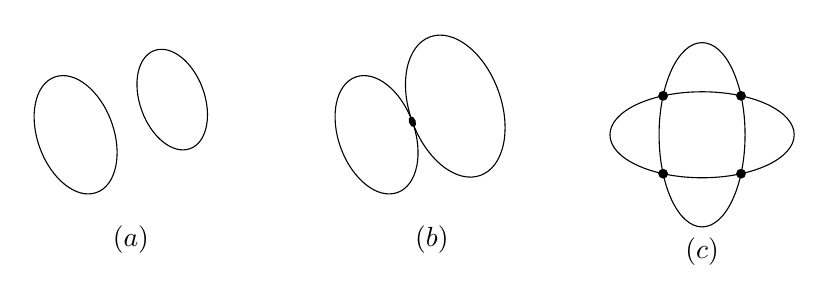
\begin{tikzpicture}[scale=0.78]
		% (a) 相离: 两椭圆无公共点
		\begin{scope}[rotate=20, xscale=0.62]
			\draw (0,0) circle (1);
			\draw (2.7,0) circle (0.85);
		\end{scope}
		\node at (0.9,-1.7) {$(a)$};
		% (b) 相切: 恰有一个公共点
		\begin{scope}[shift={(4.9,0)}, rotate=20, xscale=0.62]
			\draw (0,0) circle (1);
			\draw (2.2,0) circle (1.2);
			\fill (1.0,0) circle (0.09);
		\end{scope}
		\node at (5.8,-1.7) {$(b)$};
		% (c) 相交: 四个公共点
		\begin{scope}[shift={(10.2,0)}]
			\draw (0,0) ellipse (1.5 and 0.7);
			\draw (0,0) ellipse (0.7 and 1.5);
			\fill (0.634,0.634) circle (0.08);
			\fill (-0.634,0.634) circle (0.08);
			\fill (0.634,-0.634) circle (0.08);
			\fill (-0.634,-0.634) circle (0.08);
		\end{scope}
		\node at (10.2,-1.9) {$(c)$};
	\end{tikzpicture}
	\caption{二次曲线的相交}
	\label{fig:1.1}
\end{figure}

以下我们始终假设 $k$ 是代数闭域; 若非如此, 我们总会明确说明. 这并不意味着代数几何不适用于研究涉及非代数闭域 $k_0$ 的问题, 只是这类应用多半需要过渡到包含 $k_0$ 的某个代数闭域 $k$. 对 $\R$ 而言, 我们过渡到复数域 $\CC$.

这常常使我们能够猜测或证明一些纯实数的关系式. 下面就是这方面最初等的例子. 设 $P$ 是圆 $C$ 外一点, 则过 $P$ 可作 $C$ 的两条切线\index{qiexian@切线}.

\begin{definition}[极线]\label{def:polar-line}
	连接上述两切点的直线称为 $P$ 关于 $C$ 的\emph{极线}\index{jixian@极线}（图~\ref{fig:1.2}, (a)）.
\end{definition}

上述全部构造都可以表达为 $P$ 的坐标与 $C$ 的方程之间的代数关系式, 因此当 $P$ 位于 $C$ 内部时它们同样适用. 当然, 这时切线的切点具有复坐标, 在图上是看不到的.

但由于原始数据都是实的, 所得到的点集（即两个切点）在把所有数换成其复共轭之后应当保持不变; 也就是说, 这两个切点互为复共轭. 于是连接它们的直线 $L$ 是实的. 这条直线同样称为 $P$ 关于 $C$ 的极线.

它也容易给出一个纯实数的定义: 它是圆外那些极线通过 $P$ 的点所组成的轨迹（图~\ref{fig:1.2}, (b)）.

\begin{figure}[htbp]
	\centering
	\begin{tikzpicture}[scale=0.92]
		% (a) P 在圆外: 两条切线, 极线为切点弦
		\begin{scope}
			\draw (0,0) circle (1);
			\node at (-0.72,0.72) {$C$};
			\coordinate (T1) at (0.5,0.866);
			\coordinate (T2) at (0.5,-0.866);
			\coordinate (P) at (2,0);
			\draw (P) -- (T1);
			\draw (P) -- (T2);
			\draw[dashed] (0.5,-1.5) -- (0.5,1.5);
			\fill (T1) circle (0.04) node[above left=-2pt] {$T_1$};
			\fill (T2) circle (0.04) node[below left=-2pt] {$T_2$};
			\fill (P) circle (0.045) node[right] {$P$};
		\end{scope}
		\node at (0.75,-2.05) {$(a)$};
		% (b) P 在圆内: 极线 L 为圆外点的极线轨迹
		\begin{scope}[shift={(7.2,0)}]
			\draw (0,0) circle (1);
			\node at (-0.72,0.72) {$C$};
			\coordinate (P) at (0.5,0);
			\draw[dashed] (2,-1.5) -- (2,1.6);
			\node[above] at (2,1.6) {$L$};
			\coordinate (Q) at (2,0.8);
			\coordinate (U1) at (0.76,-0.65);
			\coordinate (U2) at (0.10,0.99);
			\draw (Q) -- (U1);
			\draw (Q) -- (U2);
			\draw[thin] (U1) -- (U2);	% Q 的极线, 恰通过 P
			\fill (P) circle (0.045) node[below=1pt] {$P$};
			\fill (Q) circle (0.045) node[right] {$Q$};
			\fill (U1) circle (0.04);
			\fill (U2) circle (0.04);
		\end{scope}
		\node at (8.0,-2.05) {$(b)$};
	\end{tikzpicture}
	\caption{点关于二次曲线的极线}
	\label{fig:1.2}
\end{figure}

下面再举几种会出现非代数闭域上代数几何问题的情形, 对它们的研究通常也需要过渡到代数闭域.

\begin{compactenum}[(1)]
	\item $k = \Q$. 研究代数曲线 $f(x,y) = 0$ 上坐标属于 $\Q$ 的点, 其中 $f \in \Q[x,y]$, 点的坐标取在 $\Q$ 中. 这是数论的基本问题之一, 即不定方程\index{bu ding fangcheng@不定方程}理论.

	例如, \trFermat{}大定理\index{Feima dadingli@费马大定理}要求我们描述曲线 $x^n + y^n = 1$ 上的点 $(x,y) \in \Q^2$.
	\item 有限域. 设 $k = \F_p$ 是模 $p$ 的剩余类域. 研究 $f(x,y) = 0$ 所确定的代数曲线上坐标属于 $k$ 的点, 是数论中的又一个问题: 同余方程 $f(x,y) \equiv 0 \pmod{p}$ 的求解.
	\item $k = \CC(z)$. 考虑 $\A^3$ 中由 $F(x,y,z) = 0$ 给出的代数曲面, 其中 $F(x,y,z) \in \CC[x,y,z]$.

	把 $z$ 放进系数, 把 $F$ 看成 $x, y$ 的多项式, 我们就可以把这张曲面视为 $z$ 的有理函数域 $\CC(z)$ 上的一条曲线. 这是研究代数曲面的一个极为有效的方法.
\end{compactenum}

\subsection{有理曲线}

众所周知, 由
\begin{equation}
	\label{eq:1.2}
	y^2 = x^2 + x^3
\end{equation}
给出的曲线具有这样的性质: 其上点的坐标可以表为一个参数的有理函数. 为推导出这些表达式, 注意过原点的直线 $y = tx$ 与曲线 \eqref{eq:1.2} 在原点之外只交于一点. 事实上, 把 $y = tx$ 代入 \eqref{eq:1.2}, 得 $x^2(t^2 - x - 1) = 0$; 其中的二重根 $x = 0$ 对应原点 $0 = (0,0)$.

除此之外还有另一个根 $x = t^2 - 1$; 由直线方程得 $y = t(t^2 - 1)$. 这样就得到所需的参数化
\begin{equation}
	\label{eq:1.3}
	x = t^2 - 1, \quad y = t(t^2 - 1),
\end{equation}
其几何意义是明显的: $t$ 是过 $0$ 与 $(x,y)$ 的直线的斜率, 而 $(x,y)$ 是直线 $y = tx$ 与曲线 \eqref{eq:1.2} 在 $0$ 之外的交点的坐标.

再换一个更直观的看法: 另取一条不经过 $0$ 的直线（例如直线 $x = 1$）, 从 $0$ 出发把曲线投影到这条直线上, 即把曲线上的点 $P$ 送到直线 $0P$ 与该直线的交点 $Q$（见图~\ref{fig:1.3}）. 这里参数 $t$ 起着该直线上坐标的作用. 由这一几何描述, 或者直接由 \eqref{eq:1.3}, 都可以看出 $t$ 由点 $(x,y)$ 唯一确定（当 $x \ne 0$ 时）.

\begin{figure}[htbp]
	\centering
	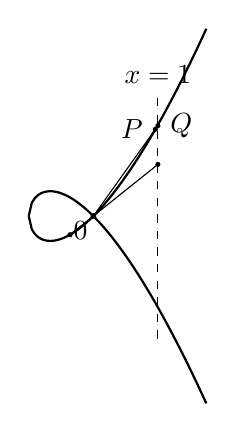
\begin{tikzpicture}[scale=0.82]
		% 三次曲线 y^2 = x^2 + x^3 的两支
		\draw[thick] plot[domain=-1:1.75, samples=60] (\x, {\x*sqrt(1+\x)});
		\draw[thick] plot[domain=-1:1.75, samples=60] (\x, {-\x*sqrt(1+\x)});
		% 投影直线 x=1
		\draw[dashed] (1,-1.9) -- (1,1.9);
		\node[above] at (1,1.9) {$x=1$};
		% 原点
		\fill (0,0) circle (0.045) node[below left=-2pt] {$0$};
		% 射线: t=1.4, P=(0.96,1.344), Q=(1,1.4)
		\draw (0,0) -- (1,1.4);
		\fill (0.96,1.344) circle (0.04) node[left=1pt] {$P$};
		\fill (1,1.4) circle (0.04) node[right=1pt] {$Q$};
		% 射线: t=0.8, P=(-0.36,-0.288), Q=(1,0.8) (P 在反向延长线上)
		\draw (-0.36,-0.288) -- (1,0.8);
		\fill (-0.36,-0.288) circle (0.04);
		\fill (1,0.8) circle (0.04);
	\end{tikzpicture}
	\caption{三次曲线的投影}
	\label{fig:1.3}
\end{figure}

现在给出一个一般的定义, 以概括那些可以用这种方式表示的代数平面曲线.

\begin{definition}[有理曲线]\label{def:rational-curve}
	设 $X$ 是由 $f(x,y) = 0$ 定义的不可约代数曲线. 如果存在两个有理函数 $\varphi(t)$ 与 $\psi(t)$, 其中至少一个非常数, 使得
	\begin{equation}
		\label{eq:1.4}
		f(\varphi(t), \psi(t)) \equiv 0
	\end{equation}
	作为 $t$ 的恒等式成立, 就称 $X$ 为\emph{有理曲线}\index{youli quxian@有理曲线}.
\end{definition}

显然, 若 $t = t_0$ 是参数的一个取值, 且不是使 $\varphi$ 或 $\psi$ 的分母为零的那有限多个值之一, 则 $(\varphi(t_0), \psi(t_0))$ 是 $X$ 的点.

我们以后将证明: 对于适当选取的参数化 $\varphi, \psi$, 映射 $t_0 \mapsto (\varphi(t_0), \psi(t_0))$ 是 $t$ 的取值与曲线的点之间的一一对应, 只需从 $t$ 的取值集合与曲线的点集中各去掉某个有限集. 反过来, 参数 $t$ 也可以表为坐标 $x, y$ 的有理函数 $t = \chi(x,y)$.

若有理函数 $\varphi$ 与 $\psi$ 的系数属于 $k$ 的某个子域 $k_0$, 且 $t_0 \in k_0$, 则点 $(\varphi(t_0), \psi(t_0))$ 的坐标也属于 $k_0$. 这一观察指出了有理曲线概念的一个可能应用. 设 $f(x,y)$ 的系数是有理数; 如果我们知道由 \eqref{eq:1.1} 给出的曲线是有理的, 并且 $\varphi$ 与 $\psi$ 的系数属于 $\Q$, 那么当 $t$ 取遍全部有理值时, 参数化 $x = \varphi(t), y = \psi(t)$ 就给出这条曲线的全部有理点\index{youli dian@有理点}, 至多除去有限多个.

例如, 当 $t$ 取遍全部有理值时, 不定方程 \eqref{eq:1.2} 的全部有理数解都可以由 \eqref{eq:1.3} 得到.

有理曲线的另一应用与积分学有关. 把曲线 \eqref{eq:1.1} 的方程看成确定了 $y$ 是 $x$ 的代数函数, 则任一有理函数 $g(x,y)$ 都是 $x$ 的（通常是复杂的）函数. 曲线 \eqref{eq:1.1} 的有理性蕴含以下重要事实: 对任一有理函数 $g(x,y)$, 不定积分
\begin{equation}
	\label{eq:1.5}
	\int g(x,y) \, dx
\end{equation}
可以用初等函数表出.

事实上, 既然曲线有理, 它就可以参数化为 $x = \varphi(t),\ y = \psi(t)$, 其中 $\varphi, \psi$ 是有理函数. 把这些表达式代入积分 \eqref{eq:1.5}, 就把它化为 $\int g(\varphi(t), \psi(t))\, \varphi'(t)\, dt$ 的形式, 这是一个有理函数的积分. 众所周知, 这种形式的积分可以用初等函数表出. 再把参数的表达式 $t = \chi(x,y)$ 代入, 便得到积分 \eqref{eq:1.5} 作为坐标的初等函数的表达式.

现在给出有理曲线的一些例子. $1$ 次曲线, 即直线, 显然是有理的.

\begin{example}[不可约二次曲线是有理的]\label{exam:conic-rational}
	取 $X$ 上一点 $(x_0, y_0)$. 考虑过 $(x_0, y_0)$ 而斜率为 $t$ 的直线, 其方程为
	\begin{equation}
		\label{eq:1.6}
		y - y_0 = t(x - x_0).
	\end{equation}
	我们来求 $X$ 与这条直线的交点: 为此从 \eqref{eq:1.6} 解出 $y$, 代入 $X$ 的方程, 得到关于 $x$ 的方程
	\begin{equation}
		\label{eq:1.7}
		f\bigl(x,\, y_0 + t(x - x_0)\bigr) = 0,
	\end{equation}
	容易看出它是 $2$ 次的. 这个二次方程有一个根是已知的, 即 $x = x_0$, 因为按照假设, $(x_0, y_0)$ 在曲线上. 用 $x^2$ 的系数去除 \eqref{eq:1.7}, 把所得方程中 $x$ 的系数记作 $A$, 则另一根由 $x + x_0 = -A$ 确定.

	由于 $t$ 出现在 \eqref{eq:1.7} 的系数中, $A$ 是 $t$ 的有理函数. 把表达式 $x = -x_0 - A$ 代入 \eqref{eq:1.6}, 就得到 $y$ 的表达式, 它同样是 $t$ 的有理函数. 从推导过程可以看出, $x, y$ 的这些表达式满足曲线的方程, 这就证明了曲线是有理的.
\end{example}

上述参数化有一个明显的几何解释: $X$ 的点 $(x,y)$ 对应连接该点与 $(x_0, y_0)$ 的直线的斜率; 参数 $t$ 对应曲线与过 $(x_0, y_0)$ 而斜率为 $t$ 的直线的交点. 这个交点之所以是唯一确定的, 正是因为我们所处理的是 $2$ 次不可约曲线. 与曲线 \eqref{eq:1.2} 的参数化的情形一样, 这一参数化可以解释为 $X$ 从点 $(x_0, y_0)$ 到某条不经过该点的直线的投影（图~\ref{fig:1.4}）.

\begin{figure}[htbp]
	\centering
	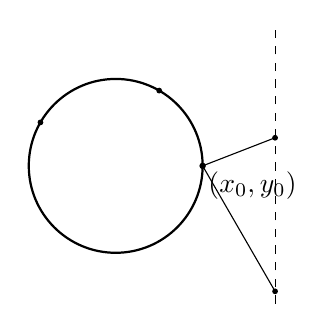
\begin{tikzpicture}[scale=0.92]
		% 二次曲线 (单位圆) 与其上一点 (x0,y0)=(1.2,0)
		\draw[thick] (0,0) circle (1.2);
		\coordinate (O1) at (1.2,0);
		\fill (O1) circle (0.045) node[below right=-2pt] {$(x_0,y_0)$};
		% 投影直线 x=2.2
		\draw[dashed] (2.2,-1.9) -- (2.2,1.9);
		% 弦 1: 过 (1.2,0) 与圆上 60° 点 (0.6,1.039), 延长交 x=2.2 于 (2.2,-1.732)
		\draw (1.2,0) -- (2.2,-1.732);
		\fill (0.6,1.039) circle (0.04);
		\fill (2.2,-1.732) circle (0.04);
		% 弦 2: 过 (1.2,0) 与圆上 150° 点 (-1.039,0.6), 延长交 x=2.2 于 (2.2,0.388)
		\draw (1.2,0) -- (2.2,0.388);
		\fill (-1.039,0.6) circle (0.04);
		\fill (2.2,0.388) circle (0.04);
	\end{tikzpicture}
	\caption{二次曲线的投影}
	\label{fig:1.4}
\end{figure}

注意, 在构造上述参数化时, 我们用到了 $X$ 上的一个点 $(x_0, y_0)$. 如果多项式 $f(x,y)$ 的系数与点 $(x_0, y_0)$ 的坐标都属于 $k$ 的某个子域 $k_0$, 那么给出参数化的那些函数的系数也属于 $k_0$. 由此, 例如只要知道一个解, 我们就能求出 $2$ 次不定方程的有理数解的一般形式.

是否存在一个解, 这个问题相当微妙. 对有理数域 $\Q$, 它由 Legendre 定理解决（例如见 Borevich--Shafarevich \cite[第 1 章 \S 7.2]{borevich-shafarevich1966}）.

再考虑所找到的参数化的另一个应用. 由刚才所证, 二次方程 $y^2 = ax^2 + bx + c$ 定义一条有理曲线. 由此可知, 对任一有理函数 $g(x,y)$, 积分 $\int g\bigl(x, \sqrt{ax^2 + bx + c}\bigr) dx$ 都可以用初等函数表出. 上面给出的参数化提供了把这一积分化为有理函数积分的那些代换的明显形式. 容易看出, 这就导出了著名的欧拉代换\index{Oula daihuan@欧拉代换}.

上面考虑的例子引出如下的一般问题: 如何判定任意一条代数平面曲线是否有理? 正如我们以后将看到的, 这个问题涉及代数几何中相当精细的思想.

\subsection{与域论的联系}

现在说明 §1.2 末尾提出的问题如何表述为一个域论问题. 为此, 我们给每条不可约平面曲线指定一个域, 就像给一元不可约多项式指定包含其一根的最小扩域那样.

设 $X$ 是由 \eqref{eq:1.1} 给出的不可约曲线. 考虑有理函数 $u(x,y) = p(x,y)/q(x,y)$, 其中 $p, q$ 是系数属于 $k$ 的多项式, 且分母 $q(x,y)$ 不被 $f(x,y)$ 整除. 我们称这样的 $u(x,y)$ 为\emph{在 $X$ 上定义的有理函数}; 而在 $X$ 上定义的两个有理函数 $p(x,y)/q(x,y)$ 与 $p_1(x,y)/q_1(x,y)$, 如果多项式 $p(x,y) q_1(x,y) - q(x,y) p_1(x,y)$ 被 $f(x,y)$ 整除, 就称它们\emph{在 $X$ 上相等}.

\begin{definition}[函数域]\label{def:function-field}
	容易验证, $X$ 上的有理函数按``在 $X$ 上相等''这一等价关系构成一个域. 这个域称为 $X$ 的\emph{函数域}\index{hanshuyu@函数域}或有理函数域, 记作 $k(X)$.
\end{definition}

有理函数 $u(x,y) = p(x,y)/q(x,y)$ 在 $X$ 上使 $q(x,y) \ne 0$ 的点处都有定义. 由于假设 $q$ 不被 $f$ 整除, 由 §1.1 的引理~\ref{lem:finite-solutions}, $u(x,y)$ 在 $X$ 上没有定义的点只有有限多个. 因此, 我们也可以把 $k(X)$ 的元素看作 $X$ 上的函数, 只是除一个有限点集外处处有定义.

可能有这样的情形: 有理函数 $u$ 有两个不同的表达式 $u = p/q$ 与 $u = p_1/q_1$, 而对某个点 $(\alpha, \beta) \in X$ 有 $q(\alpha, \beta) = 0$ 但 $q_1(\alpha, \beta) \ne 0$. 例如, 圆 $x^2 + y^2 = 1$ 上的函数 $u = (1-y)/x$ 在点 $(0,1)$ 处有另一表达式 $u = x/(1+y)$, 其分母在 $(0,1)$ 处不为零.

\begin{definition}[在一点正则]\label{def:regular-at-point}
	如果 $u$ 有一个表达式 $u = p/q$ 使得 $q(P) \ne 0$, 就称 $u$ 在点 $P$ 处\emph{正则}\index{zhengze@正则}.
\end{definition}

$k(X)$ 的每个元素显然都能写成 $x, y$ 的有理函数; 而 $x, y$ 是代数相关的, 因为它们受关系 $f(x,y) = 0$ 约束. 由此容易验证, $k(X)$ 在 $k$ 上的超越次数为 $1$.

如果 $X$ 是一条直线, 譬如由 $y = 0$ 给出, 那么 $X$ 上的每个有理函数 $\varphi(x,y)$ 只是 $x$ 的有理函数 $\varphi(x,0)$, 于是 $X$ 的函数域就是一元有理函数域: $k(X) = k(x)$.

现在设曲线 $X$ 是有理的, 譬如参数化为 $x = \varphi(t),\ y = \psi(t)$. 考虑代换 $u(x,y) \mapsto u(\varphi(t), \psi(t))$, 它把 $X$ 上的任一有理函数 $u = p(x,y)/q(x,y)$ 送到把 $x$ 换成 $\varphi(t)$, 把 $y$ 换成 $\psi(t)$ 之后所得的 $t$ 的有理函数.

我们先验证这个代换有意义, 也就是分母 $q(\varphi(t), \psi(t))$ 作为 $t$ 的函数不恒为零. 假设 $q(\varphi(t), \psi(t)) = 0$, 把它与 \eqref{eq:1.4} 比较. 注意域 $k$ 是代数闭的, 因而是无限域; 让 $t$ 在 $k$ 中取不同的值, 便知 $f(x,y) = 0$ 与 $q(x,y) = 0$ 有无穷多个公共解. 但由 §1.1 的引理~\ref{lem:finite-solutions}, 这只有当 $f$ 与 $q$ 有公因子时才可能发生.

因此, 我们的代换把 $X$ 上定义的任一有理函数 $u(x,y)$ 送到 $k(t)$ 中的一个良定义的元素. 此外, 由于 $\varphi$ 与 $\psi$ 满足关系 \eqref{eq:1.4}, 在 $X$ 上相等的有理函数 $u$ 与 $u_1$ 被送到同一个 $t$ 的有理函数. 这样, $k(X)$ 的每个元素都对应到 $k(t)$ 中一个良定义的元素. 这一映射显然给出 $k(X)$ 与 $k(t)$ 的某个子域的同构, 并且把 $k$ 中的元素映为其自身.

这里我们要用到关于有理函数的一个定理, 即如下的 Lüroth 定理\index{Lüroth dingli@Lüroth 定理}: 有理函数域 $k(t)$ 的包含 $k$ 的子域必定形如 $k(g(t))$, 其中 $g(t)$ 是某个有理函数; 也就是说, 这个子域由 $g(t)$ 的全体有理函数组成. 若 $g(t)$ 不是常数, 则对应 $f(u) \mapsto f(g(t))$ 显然给出有理函数域 $k(u)$ 与 $k(g(t))$ 的同构. 因此 Lüroth 定理又可以叙述为: 有理函数域 $k(t)$ 的包含 $k$ 而不等于 $k$ 的子域, 本身同构于有理函数域. Lüroth 定理可以由域扩张的简单性质证明（见 van der Waerden \cite[10.2, \S 73]{vdw1991}）.

把它应用到我们的情形: 若 $X$ 是有理曲线, 则 $k(X)$ 同构于有理函数域 $k(t)$. 反之, 设对某条由 \eqref{eq:1.1} 给出的曲线 $X$, 域 $k(X)$ 同构于有理函数域 $k(t)$; 设在此同构下 $x$ 对应 $\varphi(t)$, $y$ 对应 $\psi(t)$. $k(X)$ 中的多项式关系 $f(x,y) = 0$ 在域同构下保持, 给出 $f(\varphi(t), \psi(t)) = 0$; 因此 $X$ 是有理曲线.

容易看出, 任何包含 $k$, 在 $k$ 上超越次数为 $1$, 且由两个元素 $x, y$ 生成的域 $K$, 都同构于某个域 $k(X)$, 其中 $X$ 是一条不可约代数平面曲线. 事实上, 既然 $K$ 在 $k$ 上超越次数为 $1$, $x$ 与 $y$ 必然由某个多项式关系联系; 设这个关系为 $f(x,y) = 0$, 其中 $f$ 是不可约多项式, 那么显然可以取 $X$ 为这个方程所定义的代数曲线.

由此, §1.2 末尾提出的关于有理曲线的问题, 就等价于下述域论问题: 包含 $k$, 在 $k$ 上超越次数为 $1$ 且由两个元素 $x, y$ 生成的域 $K$, 何时同构于一元有理函数域 $k(t)$? 从代数的观点看, ``由两个元素生成''这一要求并不很自然; 更自然的是考虑由任意有限多个元素生成的域扩张. 不过, 我们以后将证明, 这样做并不会得到更一般的概念（比较定理 1.8 与命题 A.7\footnote{此处沿用原书编号, 待相应部分译出后改为内部交叉引用.}）.

最后我们指出, 前面的论证使我们能够解决求有理曲线的（除有限点外一一的）参数化的问题. 设 $X$ 是有理曲线. 由 Lüroth 定理, 域 $k(X)$ 同构于有理函数域 $k(t)$. 设此同构把 $x$ 映为 $\varphi(t)$, 把 $y$ 映为 $\psi(t)$, 这就给出了 $X$ 的参数化 $x = \varphi(t),\ y = \psi(t)$.

\begin{proposition}\label{prop:generic-bijection}
	参数化 $x = \varphi(t),\ y = \psi(t)$ 具有下列性质:
	\begin{compactenum}[(i)]
		\item 除有限多个点外, 任一点 $(x_0, y_0) \in X$ 都可表为 $(x_0, y_0) = (\varphi(t_0), \psi(t_0))$, 其中 $t_0$ 是某个参数值;
		\item 除有限多个点外, 这种表示是唯一的.
	\end{compactenum}
\end{proposition}

\begin{proof}
	设在同构 $k(X) \to k(t)$ 之下映到 $t$ 的函数是 $\chi(x,y)$, 则逆同构 $k(t) \to k(X)$ 由公式 $u(t) \mapsto u(\chi(x,y))$ 给出. 把``两个对应互逆''写出来, 就是
	\begin{equation}
		\label{eq:1.8}
		x = \varphi(\chi(x,y)), \quad y = \psi(\chi(x,y)),
	\end{equation}
	\begin{equation}
		\label{eq:1.9}
		t = \chi(\varphi(t), \psi(t)).
	\end{equation}

	由 \eqref{eq:1.8} 立即得到 (i). 事实上, 设 $\chi(x,y) = p(x,y)/q(x,y)$ 且 $q(x_0, y_0) \ne 0$, 则可取 $t_0 = \chi(x_0, y_0)$; 由于 $q(x,y)$ 与 $f(x,y)$ 互素, 使 $q(x_0, y_0) = 0$ 的点 $(x_0, y_0) \in X$ 只有有限多个. 再设 $(x_0, y_0)$ 满足: $\chi(x_0, y_0)$ 不是 $\varphi(t)$ 与 $\psi(t)$ 的分母的根; 由同样的理由, 不满足这一条件的点也只有有限多个. 于是 \eqref{eq:1.8} 就给出 $(x_0, y_0)$ 的所需表示.

	同样, 由 \eqref{eq:1.9} 可知, 若参数值 $t$ 存在, 则它由点 $(x_0, y_0)$ 唯一确定, 至多除去使 $q(x_0, y_0) = 0$ 的那有限多个点. 命题证毕.
\end{proof}

\begin{remark}\label{rem:param-not-unique}
	注意, 我们证明的 (i) 与 (ii) 并非对有理曲线的任何参数化都成立, 而只是对上面特别构造的参数化成立. 对随意取的参数化, (ii) 可能不成立: 例如, 曲线 \eqref{eq:1.2} 除 \eqref{eq:1.3} 给出的参数化外, 还有参数化 $x = t^4 - 1,\ y = t^2(t^4 - 1)$, 它是把 \eqref{eq:1.3} 中的 $t$ 换成 $t^2$ 得到的. 显然, 此时参数值 $t$ 与 $-t$ 对应曲线上的同一个点.
\end{remark}

\subsection{有理映射}

\begin{definition}[有理映射]\label{def:rational-map}
	设 $X$ 与 $Y$ 是两条不可约代数平面曲线, $u, v \in k(X)$. 映射 $\varphi(P) = (u(P), v(P))$ 在使 $u$ 与 $v$ 都有定义的所有点 $P \in X$ 上有定义; 如果在 $\varphi$ 有定义的每一点 $P \in X$ 处都有 $\varphi(P) \in Y$, 就称 $\varphi$ 为从 $X$ 到 $Y$ 的\emph{有理映射}\index{youli yingshe@有理映射}. 若 $Y$ 的方程为 $g = 0$, 则 $g(u,v) \in k(X)$ 必在 $X$ 上除有限多个点外处处取零, 因而在 $k(X)$ 中必须有 $g(u,v) = 0$.
\end{definition}

例如, §1.2 中考虑的从点 $P$ 出发的投影是从 $X$ 到直线的一个有理映射; 有理曲线 $X$ 的有理参数化是从直线到 $X$ 的有理映射.

\begin{definition}[双有理映射]\label{def:birational}
	有理映射 $\varphi: X \to Y$ 称为\emph{双有理的}, 或称为 $X$ 到 $Y$ 的\emph{双有理等价}\index{shuangyouli@双有理等价}, 如果 $\varphi$ 有有理逆, 即存在有理映射 $\psi: Y \to X$, 使得 $\varphi \circ \psi$ 与 $\psi \circ \varphi$（在它们有定义的点处）都是恒等映射. 这时称 $X$ 与 $Y$ 是双有理的, 或双有理等价的.
\end{definition}

双有理映射不是常数映射, 也就是说, 定义它的函数中至少有一个不属于 $k$. 事实上, 常数映射处处有定义, 且把 $X$ 映到 $Y$ 的单独一点 $Q$; 取 $\varphi$ 的逆 $\psi$ 有定义的任一点 $Q' \ne Q$, 便与定义相矛盾.

由此还可得出: 对任一点 $Q \in Y$, 双有理映射下 $Q$ 的原像 $\varphi^{-1}(Q)$（即满足 $\varphi(P) = Q$ 的点 $P \in X$ 组成的集合）是有限集; 这由 §1.1 的引理~\ref{lem:finite-solutions} 立得. 设 $S$ 是 $X$ 上使双有理映射 $\varphi: X \to Y$ 无定义的点组成的有限集, $U = X \setminus S$ 为其补集; $T$ 与 $V$ 是关于 $\psi: Y \to X$ 的相应集合. 由上面所述, $\varphi^{-1}(V) \cap U$ 在 $X$ 中的补集与 $\psi^{-1}(U) \cap V$ 在 $Y$ 中的补集都是有限集, 并且 $\varphi$ 给出 $\varphi^{-1}(V) \cap U$ 与 $\psi^{-1}(U) \cap V$ 之间的一一对应.

双有理等价是代数几何中的基本等价关系, 我们通常把代数曲线按双有理等价来分类. 我们已经看到, 有理曲线恰好是与直线双有理等价的那些曲线.

设 $n$ 次不可约曲线的方程 $f(x,y)$ 的各项都是 $x, y$ 的次数为 $n-1$ 或 $n$ 的单项式, 那么从原点出发的投影给出这条曲线与直线之间的双有理映射; 把关于曲线 \eqref{eq:1.2} 的论证直接推广即可证明这一点.

再设 $f$ 含有次数分别为 $n-2, n-1$ 与 $n$ 的项, 即 $f = u_{n-2} + u_{n-1} + u_n$, 其中 $u_i$ 是 $i$ 次齐次多项式. 仍令 $y = tx$, 从方程中约去因子 $x^{n-2}$, 把它化为
\[
	a(t)\, x^2 + b(t)\, x + c(t) = 0,
\]
其中 $a(t) = u_n(1,t),\ b(t) = u_{n-1}(1,t),\ c(t) = u_{n-2}(1,t)$. 令 $s = 2ax + b$ 以配方（设基域特征 $\ne 2$）, 便见我们的曲线与由 $s^2 = p(t)$ 给出的曲线双有理等价, 其中 $p = b^2 - 4ac$.

\begin{definition}[超椭圆曲线]\label{def:hyperelliptic}
	上述 $s^2 = p(t)$ 型的曲线称为\emph{超椭圆曲线}\index{chao tuoyuan quxian@超椭圆曲线}.
\end{definition}

若 $p(t)$ 的次数是偶数 $2m$, 则把 $p(t)$ 写成 $p(t) = q(t)(t - \alpha)$, 并把方程两边同除以 $(t-\alpha)^{2m}$, 便知该曲线与由
\[
	\eta^2 = h(\xi), \quad \text{其中}\ \xi = \frac{1}{t - \alpha},\ \ \eta = \frac{s}{(t-\alpha)^m},\ \ h(\xi) = \frac{q(t)}{(t-\alpha)^{2m-1}}
\]
给出的曲线双有理等价, 其中 $h$ 是 $\xi$ 的次数 $\le 2m-1$ 的多项式.

这些想法特别适用于任何一条三次曲线, 只需把原点取为曲线上的任一点. 于是我们看到: 当 $\operatorname{char} k \ne 2$ 时, 任何不可约三次曲线都双有理等价于由 $y^2 = f(x)$ 给出的曲线, 其中 $f$ 是次数 $\le 3$ 的多项式. 若 $f(x)$ 的次数 $\le 2$, 则该三次曲线是有理的; 若次数为 $3$, 则可设其首项系数为 $1$, 于是方程化为
\[
	y^2 = x^3 + ax^2 + bx + c.
\]

\begin{definition}[Weierstrass 标准型]\label{def:weierstrass}
	上式称为三次曲线方程的\emph{Weierstrass 标准型}. 若 $\operatorname{char} k \ne 3$, 则经过平移 $x \mapsto x - a/3$ 可把方程化为
	\begin{equation}
		\label{eq:1.10}
		y^2 = x^3 + px + q.
	\end{equation}
\end{definition}

设 $X$ 与 $Y$ 是两条双有理等价的不可约代数平面曲线, 其间的映射由
\[
	(u, v) = \bigl(\varphi(x,y),\, \psi(x,y)\bigr) \quad\text{与}\quad (x, y) = \bigl(\xi(u,v),\, \eta(u,v)\bigr)
\]
给出. 与有理曲线的研究相同, 我们可以建立这两条曲线的函数域 $k(X)$ 与 $k(Y)$ 之间的联系: 把有理函数 $w(x,y) \in k(X)$ 送到 $w(\xi(u,v), \eta(u,v))$, 视为 $Y$ 上的有理函数. 容易验证, 这定义了一个映射 $k(X) \to k(Y)$, 并且是这两个域之间的同构.

反之, 设 $k(X)$ 与 $k(Y)$ 同构. 在此同构下, $x, y \in k(X)$ 对应于 $\xi(u,v), \eta(u,v) \in k(Y)$, 而 $u, v \in k(Y)$ 对应于 $\varphi(x,y), \psi(x,y) \in k(X)$.

同样容易逐条验证, 函数对 $\varphi, \psi$ 与 $\xi, \eta$ 给出曲线 $X$ 与 $Y$ 之间的双有理映射.

因此, 两条曲线双有理等价, 当且仅当它们的有理函数域同构.

我们看到, 代数曲线按双有理等价分类的问题, 是把 $k$ 上超越次数为 $1$ 的有限生成扩域按同构分类这一自然代数问题的几何侧面. 在这个问题中, 不把讨论局限于超越次数为 $1$ 的域, 而考虑任意有限超越次数的域, 同样是自然的. 以后我们将看到, 问题的这种更广提法也有几何解释; 但为此必须走出代数曲线理论的框架, 考虑任意维数的代数簇.

\subsection{奇异点与非奇异点}

\begin{definition}[奇异点]\label{def:singular-point}
	我们从坐标几何借用一个定义: 若
	\[
		f'_x(P) = f'_y(P) = f(P) = 0
	\]
	（$f'_x$ 表示偏导数 $\partial f / \partial x$）, 就称点 $P$ 为曲线 $f(x,y) = 0$ 的\emph{奇异点}\index{qiyi dian@奇异点}或奇点. 不是奇点的点称为\emph{非奇异的}, 即满足 $f'_x(P) \ne 0$ 或 $f'_y(P) \ne 0$ 的点. 所有点都非奇异的曲线称为\emph{非奇异的}或\emph{光滑的}.
\end{definition}

把 $P$ 平移到原点, 就可以说: $(0,0)$ 是奇点, 当且仅当 $f$ 不含常数项和一次项. 众所周知, 不可约二次曲线是非奇异的; 奇异曲线最简单的例子是曲线 \eqref{eq:1.2}.

对不可约曲线而言, 或者 $f'_x$ 只在曲线的有限多个点上为零, 或者 $f'_x$ 被 $f$ 整除. 但 $f'_x$ 的次数小于 $f$ 的次数, 故后一情形仅当 $f'_x = 0$ 时才可能. 对 $f'_y$ 同理. 然而 $f'_x = f'_y = 0$ 蕴含: 当 $\operatorname{char} k = 0$ 时 $f \in k$; 当 $\operatorname{char} k = p > 0$ 时, $f$ 中的 $x$ 与 $y$ 只以 $p$ 次幂出现. 在后一情形, 对 $f$ 的系数取 $p$ 次根, 并利用熟知的特征 $p$ 恒等式 $(\alpha + \beta)^p = \alpha^p + \beta^p$, 便得
\[
	f = \sum a_{ij}\, x^{pi} y^{pj} = \Bigl( \sum b_{ij}\, x^i y^j \Bigr)^{p}, \quad \text{其中 } b_{ij}^{\,p} = a_{ij},
\]
这与曲线的不可约性矛盾. 于是, 不可约曲线只有有限多个奇异点.

\begin{definition}[重数]\label{def:multiplicity-point}
	设 $P = (0,0)$, 且曲线方程中最低次项的次数为 $r$, 则称 $r$ 为点 $P$ 的\emph{重数}, 称 $P$ 为 $r$ 重点. 于是非奇异点的重数为 $1$.
\end{definition}

设 $P = (0,0)$ 的重数为 $2$, 且方程的二次部分为 $ax^2 + bxy + cy^2$, 则有两种可能: (a) $ax^2 + bxy + cy^2$ 分解为两个不同的一次因式之积; (b) $ax^2 + bxy + cy^2$ 是完全平方. 情形 (a) 中的奇点称为\emph{结点}（见图~\ref{fig:1.3}）, 情形 (b) 中的称为\emph{尖点}（图~\ref{fig:1.5}）.

\begin{figure}[htbp]
	\centering
	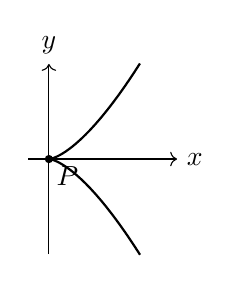
\begin{tikzpicture}[scale=1.05]
		\draw[->] (-0.25,0) -- (1.55,0) node[right] {$x$};
		\draw[->] (0,-1.15) -- (0,1.15) node[above] {$y$};
		\draw[thick] plot[domain=-1.05:1.05, samples=50] ({\x*\x}, {\x*\x*\x});
		\fill (0,0) circle (0.05) node[below right=-1pt] {$P$};
	\end{tikzpicture}
	\caption{尖点}
	\label{fig:1.5}
\end{figure}

由定义, $n$ 次曲线不可能有重数 $> n$ 的奇点. 若某奇点的重数为 $n$, 则曲线的方程是 $n$ 次齐次多项式, 从而分解为一次因式之积, 于是曲线是可约的. 在 §1.4 中我们证明了: $n$ 次不可约曲线若有 $n-1$ 重点则是有理的, 若有 $n-2$ 重点则是超椭圆的. 写成 Weierstrass 标准型 \eqref{eq:1.10} 的三次曲线是非奇异的, 当且仅当右端的三次多项式没有重根, 也就是 $4p^3 + 27q^2 \ne 0$.

\begin{definition}[椭圆曲线]\label{def:elliptic-curve}
	这时（即曲线非奇异时）, 称该曲线为\emph{椭圆曲线}\index{tuoyuan quxian@椭圆曲线}.
\end{definition}

设 $k = \R$, $P$ 是曲线 $f(x,y) = 0$ 的非奇异点, 并且（不妨设）$f'_y(P) \ne 0$. 由隐函数定理, 在 $P$ 的某个邻域内可以把 $y$ 写成 $x$ 的函数. 代入这个表达式, 便把曲线上的任何有理函数在 $P$ 附近表示成了 $x$ 的函数.

当 $k$ 是一般的域时, 仍可以用 $x$ 来描述曲线上的全部有理函数, 只是程度要有限一些. 为简单起见设 $P = (0,0)$. 此时 $f = \alpha x + \beta y + g$, 其中 $g$ 只含次数 $\ge 2$ 的项, 且 $\beta \ne 0$. 把 $f$ 中只含 $x$ 的项归并出来, 写 $f = x\varphi(x) + y\beta + yh$, 其中 $h(0,0) = 0$. 于是在曲线 $f = 0$ 上有 $y(\beta + h) = -x\varphi(x)$; 换言之, $y = xv$, 其中 $v = -\varphi(x)/(\beta + h)$ 是在 $P$ 正则的函数（因为 $\beta + h(P) \ne 0$）.

设 $u$ 是曲线上任一在 $P$ 正则且 $u(P) = 0$ 的有理函数. 写 $u = p/q$, 其中 $p, q \in k[x,y]$, $p(P) = 0$ 而 $q(P) \ne 0$. 把 $y$ 的上述表达式代入, 得 $p(x,y) = p(x, xv) = x^r$（因为 $p$ 没有常数项）, 其中 $r$ 是曲线上的正则函数, 于是 $u = x^r / q = x u_1$. 若 $u_1(P) = 0$, 则可重复论证而得 $u = x^2 u_2$, 如此等等. 我们现在证明: 只要 $u$ 不在曲线上恒为零, 这一过程必在有限多步后停止.

为此回到表达式 $u = p/q$, 其中按假设 $p$ 不被 $f$ 整除. 于是存在 $\xi, \eta \in k[x,y]$ 与多项式 $a \in k[x]$, $a \ne 0$, 使得 $f\xi + p\eta = a$（在 §1.1 引理的证明中已经用过这一论证）. 设 $a = x^k a_0$ 而 $a_0(0) \ne 0$. 在曲线上有 $p\eta = a$; 若有表示 $p = x^l w$ 而 $l > k$, 便得矛盾: 在曲线上 $x^k (x^{l-k} w - a_0) = 0$, 亦即 $x^{l-k} w - a_0 = 0$. 记 $w = c/d$, 其中 $c, d \in k[x,y]$ 且 $d(P) \ne 0$, 则 $x^{l-k} c - a_0 d$ 在曲线上为零, 即被 $f$ 整除; 但这是不可能的, 因为 $x^{l-k}$ 在 $P$ 处为零, 而 $a_0 d$ 不为零. 由于任一有理函数都是两个正则函数之比, 我们证明了下面的定理.

\begin{theorem}\label{thm:local-parameter}
	在不可约代数曲线的任一非奇异点 $P$ 处, 存在一个在 $P$ 处为零的正则函数 $t$, 使得每一个在曲线上不恒为零的有理函数 $u$ 都可以写成
	\begin{equation}
		\label{eq:1.11}
		u = t^k v
	\end{equation}
	的形式, 其中 $v$ 在 $P$ 处正则且 $v(P) \ne 0$. 函数 $u$ 在 $P$ 处正则, 当且仅当 \eqref{eq:1.11} 中 $k \ge 0$.
\end{theorem}

\begin{definition}[局部参数]\label{def:local-parameter}
	具有上述性质的函数 $t$ 称为曲线在点 $P$ 处的\emph{局部参数}\index{jubu canshu@局部参数}. 显然, 两个不同的局部参数之间有关系 $t' = tv$, 其中 $v$ 在 $P$ 处正则且 $v(P) \ne 0$. 从定理的证明中我们看到, 若 $f'_y(P) \ne 0$, 则可以取 $x$ 作为局部参数.
\end{definition}

\eqref{eq:1.11} 中的数 $k$ 称为 $u$ 在 $P$ 处零点的\emph{重数}; 它与局部参数的选取无关.

\begin{definition}[相交重数]\label{def:intersection-mult}
	设 $X$ 与 $Y$ 是方程分别为 $f = 0$ 与 $g = 0$ 的代数曲线, $X$ 不可约且不含于 $Y$ 之中, 并且 $P \in X \cap Y$ 是 $X$ 的非奇异点. 那么 $g$ 定义了 $X$ 上一个不恒为零的函数; $g$ 在 $P$ 处零点的重数称为 $X$ 与 $Y$ 在点 $P$ 处的\emph{相交重数}\index{xiangjiao chongshu@相交重数}\footnote{本书稍后将详细讨论相交重数; 一般的（对 $X$ 与 $Y$ 对称的）相交重数定义, 以及它与这里所用的简单定义的一致性, 见原书第 4 章第 1 节（暂按原书编号）.}.
\end{definition}

相交重数的概念, 是正确陈述 Bézout 定理所需要的修正之一: ``多项式的根数等于它的次数''这一定理, 如果不把根按重数计算, 就是不成立的. 下面我们在 $X$ 是直线的情形下分析相交重数.

设 $P = (\alpha, \beta) \in X$, 把 $X$ 的方程写成 $f(x,y) = a(x-\alpha) + b(y-\beta) + g$ 的形式, 其中 $g$ 按 $x - \alpha$ 与 $y - \beta$ 的幂展开后只含次数 $\ge 2$ 的项. 把过 $P$ 的直线 $L$ 的方程写成
\begin{equation}
	\label{eq:1.12}
	x = \alpha + \lambda t, \quad y = \beta + \mu t,
\end{equation}
$t$ 是 $L$ 在 $P$ 处的局部参数. 把 $f$ 限制到 $L$ 上, 便得
\[
	f(\alpha + \lambda t,\, \beta + \mu t) = (a\lambda + b\mu)\, t + t^2 \varphi(t).
\]

由此看出: 若 $P$ 是奇点, 即 $a = b = 0$, 那么过 $P$ 的每条直线与 $X$ 在 $P$ 处的相交重数都 $> 1$. 另一方面, 若曲线非奇异, 这样的直线只有一条, 即满足 $a\lambda + b\mu = 0$ 的那条, 其方程为 $a(x-\alpha) + b(y-\beta) = 0$. 显然 $a = f'_x(P)$, $b = f'_y(P)$, 因此这个方程可以写成
\begin{equation}
	\label{eq:1.13}
	f'_x(P)\,(x - \alpha) + f'_y(P)\,(y - \beta) = 0.
\end{equation}

\begin{definition}[切线]\label{def:tangent-line}
	由方程 \eqref{eq:1.13} 给出的直线称为曲线 $X$ 在非奇异点 $P$ 处的\emph{切线}.
\end{definition}

现在来确定, 何时一条直线与曲线在非奇异点 $P = (\alpha, \beta)$ 处有相交重数 $\ge 3$. 为此把方程写成
\begin{equation}
	\label{eq:1.14}
	f(x,y) = a(x-\alpha) + b(y-\beta) + c(x-\alpha)^2 + d(x-\alpha)(y-\beta) + e(y-\beta)^2 + h,
\end{equation}
其中 $h$ 按 $x - \alpha$ 与 $y - \beta$ 的幂展开后只含次数 $\ge 3$ 的项. 把 $f$ 限制到直线 $L$（\eqref{eq:1.12}）上, 得
\[
	f = (a\lambda + b\mu)\, t + (c\lambda^2 + d\lambda\mu + e\mu^2)\, t^2 + t^3 \psi(t).
\]
因此, 相交重数 $\ge 3$ 当且仅当条件 $a\lambda + b\mu = 0$ 与 $c\lambda^2 + d\lambda\mu + e\mu^2 = 0$ 同时成立.

第一个条件如上所述, 意味着 $L$ 是 $X$ 在 $P$ 处的切线; 第二个条件意味着 $c u^2 + d u v + e v^2$ 作为 $u, v$ 的齐次多项式被 $a u + b v$ 整除. 两者合起来说明二次曲线 $q = a u + b v + c u^2 + d u v + e v^2$ 是可约的: 它被 $a u + b v$ 整除. 反之, 若 $q$ 可约, 则 $q = r s$, 其中 $r$ 与 $s$ 必是一次多项式, 且二者之一（设为 $r$）在 $u = v = 0$ 时为零; 于是 $r$ 与 $a u + b v$ 成比例, 从而 $c u^2 + d u v + e v^2$ 被 $a u + b v$ 整除.

因此, 二次曲线 $q = a u + b v + c u^2 + d u v + e v^2$ 可约, 是存在过 $P$ 且与 $X$ 在 $P$ 处相交重数 $\ge 3$ 的直线的必要且充分条件.

\begin{definition}[拐点]\label{def:flex}
	这样的点 $P$ 称为曲线 $X$ 的\emph{拐点}\index{guaidian@拐点}.
\end{definition}

我们从坐标几何已经知道二次曲线可约的条件. 设 $k$ 的特征 $\ne 2$; 注意到 $a = f'_x(P)$, $b = f'_y(P)$, $c = \tfrac{1}{2} f''_{xx}(P)$, $d = f''_{xy}(P)$ 与 $e = \tfrac{1}{2} f''_{yy}(P)$, 这个条件可以写成
\begin{equation}
	\label{eq:1.15}
	\begin{vmatrix}
		f''_{xx} & f''_{xy} & f'_x \\
		f''_{xy} & f''_{yy} & f'_y \\
		f'_x    & f'_y    & 0
	\end{vmatrix}_{(P)} = 0.
\end{equation}

\subsection{射影平面}

我们回到 §1.1 所述的 Bézout 定理. 即使考虑坐标在代数闭域中的点并把相交的重数计算在内, 该定理在非常简单的情形下仍不成立, 还需要再作一项修正. 这从两条直线的例子已经可以看出: 两条平行直线没有交点. 然而在射影平面上, 平行直线是相交的, 交点在无穷远直线上.

同样, 平面上任何两条圆周, 虽然都是 $2$ 次曲线, 却至多有 $2$ 个交点, 而不是 Bézout 定理所预言的 $4$ 个. 这是因为所有圆周方程的二次项都相同, 即 $x^2 + y^2$, 于是把一个圆的方程减去另一个的便得到线性方程, 因此两圆的相交等同于圆与直线的相交. 此外, 若两圆不相切, 则它们在每个交点处的相交重数都是 $1$.

要理解 Bézout 定理失效背后的原因, 把圆的方程 $(x-a)^2 + (y-b)^2 = r^2$ 通过 $x = \xi/\zeta,\ y = \eta/\zeta$ 改写为齐次坐标: 得 $(\xi - a\zeta)^2 + (\eta - b\zeta)^2 = r^2 \zeta^2$. 由此看出, 圆与无穷远直线 $\zeta = 0$ 交于 $\xi^2 + \eta^2 = 0$ 的点, 即交于两个虚圆点（无穷远点）$(1, \pm i, 0)$. 于是所有的圆周都共有两个无穷远点 $(1, \pm i, 0)$. 连同两个有限交点, 我们便得到 $4$ 个交点, 与 Bézout 定理相符. 这类现象促使我们从仿射平面过渡到射影平面.

\begin{definition}[射影平面与齐次坐标]\label{def:projective-plane}
	射影平面 $\PP^2$ 的点由域 $k$ 中不全为零的 $3$ 个元素 $(\xi, \eta, \zeta)$ 确定; 两个三元组 $(\xi, \eta, \zeta)$ 与 $(\xi', \eta', \zeta')$ 确定同一点, 当且仅当存在 $\lambda \in k$, $\lambda \ne 0$, 使 $\xi = \lambda\xi'$, $\eta = \lambda\eta'$ 且 $\zeta = \lambda\zeta'$. 定义点 $P$ 的任一三元组 $(\xi, \eta, \zeta)$ 称为 $P$ 的一组\emph{齐次坐标}\index{qici zuobiao@齐次坐标}, 记作 $P = (\xi : \eta : \zeta)$.
\end{definition}

有包含映射 $\A^2 \subset \PP^2$, 它把 $(x, y) \in \A^2$ 送到 $(x : y : 1)$. 这样得到的是所有 $\zeta \ne 0$ 的点: $\PP^2$ 中使 $\zeta \ne 0$ 的点 $(\xi : \eta : \zeta)$ 对应 $\A^2$ 中的点 $(\xi/\zeta,\ \eta/\zeta)$. 补集 $\zeta = 0$ 的点称为\emph{无穷远点}. 这一概念与坐标 $\zeta$ 的选取有关: $\PP^2$ 实际上以这种方式包含三个仿射平面的副本: $\A^2_1$（由 $\xi \ne 0$ 给出）, $\A^2_2$（由 $\eta \ne 0$ 给出）与 $\A^2_3$（由 $\zeta \ne 0$ 给出）.

它们当然相交: 若点 $P \in \A^2_3$ 的坐标为 $x = \xi/\zeta,\ y = \eta/\zeta$ 且 $\eta \ne 0$, 则它在 $\A^2_2$ 中有坐标 $x' = \xi/\eta,\ y' = \zeta/\eta$, 即 $x' = x/y,\ y' = 1/y$; 若 $\xi \ne 0$, 则它在 $\A^2_1$ 中有坐标 $x'' = \eta/\xi,\ y'' = \zeta/\xi$, 即 $x'' = y/x,\ y'' = 1/x$. 每个点 $P \in \PP^2$ 都至少落在 $\A^2_1, \A^2_2$ 或 $\A^2_3$ 之一中, 从而可用该副本的仿射坐标写出.

\begin{definition}[射影平面曲线]\label{def:projective-curve}
	$\PP^2$ 中的代数曲线, 即射影代数平面曲线, 由齐次坐标的方程 $F(\xi, \eta, \zeta) = 0$ 定义, 其中 $F$ 是齐次多项式. 此时 $F(\xi,\eta,\zeta) = 0$ 是否成立与该点齐次坐标的选取无关, 也就是说, 在把 $\xi, \eta, \zeta$ 换成 $\xi' = \lambda\xi$, $\eta' = \lambda\eta$, $\zeta' = \lambda\zeta$（$\lambda \ne 0$）时保持不变. 齐次多项式也称为\emph{型}.
\end{definition}

次数为 $n$ 而方程为 $f(x,y) = 0$ 的仿射代数曲线确定齐次多项式 $F(\xi, \eta, \zeta) = \zeta^n f(\xi/\zeta, \eta/\zeta)$, 从而确定方程为 $F(\xi,\eta,\zeta) = 0$ 的射影曲线. 容易看出, 这条曲线与仿射平面 $\A^2_3$ 的交正是原来的仿射曲线, 因此它只是在原曲线上添加了 $\zeta = 0$ 的无穷远点. 反之, 若射影曲线的方程为 $F(\xi,\eta,\zeta) = 0$, 则相应仿射曲线的方程是 $f(x,y) = 0$, 其中 $f(x,y) = F(x, y, 1)$.

由于每个点 $P \in \PP^2$ 都属于 $\A^2_1, \A^2_2$ 或 $\A^2_3$ 之一, 利用上述对应, 我们可以把前面对仿射曲线定义的概念用齐次坐标写出. 现在就对代数曲线的切线, 奇异点与拐点这三个概念来做这件事, 且总设 $P \in \A^2_3$.

在仿射坐标下, 切线的方程是
\[
	\frac{\partial f}{\partial x}(P)\,(x - \alpha) + \frac{\partial f}{\partial y}(P)\,(y - \beta) = 0.
\]
按假设 $f(x,y) = F(x,y,1)$, 其中 $F(\xi,\eta,\zeta) = 0$ 是曲线的齐次方程. 于是（$F'_x$ 等记偏导数）$\partial f/\partial x = F'_x(x,y,1)$, $\partial f/\partial y = F'_y(x,y,1)$; 而由关于齐次函数的熟知的 Euler 定理,
\[
	F'_\xi\, \xi + F'_\eta\, \eta + F'_\zeta\, \zeta = n F.
\]
既然 $P = (\alpha : \beta : 1)$ 在曲线上, 有 $F'_\xi(P)\,\alpha + F'_\eta(P)\,\beta + F'_\zeta(P) = 0$, 于是切线的方程为 $F'_\xi(P)\,x + F'_\eta(P)\,y + F'_\zeta(P) = 0$, 用齐次坐标写就是
\[
	F'_\xi(P)\,\xi + F'_\eta(P)\,\eta + F'_\zeta(P)\,\zeta = 0.
\]

仿射坐标下奇异点的条件是 $f'_x = f'_y = f = 0$. 于是在齐次坐标下为 $F'_\xi = F'_\eta = F = 0$; 再由 Euler 定理（此时 $\zeta = 1$）得 $F'_\zeta = 0$. 若域 $k$ 的特征为 $0$, 则只要求 $F'_\xi(P) = F'_\eta(P) = F'_\zeta(P) = 0$ 就够了, 因为由此也有 $F(P) = 0$.

拐点的条件由关系式 \eqref{eq:1.15} 给出. 这里同样有 $f(x,y) = F(x,y,1)$, 于是 $f'_x = F'_x$, $f'_y = F'_y$, $f''_{xx} = F''_{xx}$, $f''_{xy} = F''_{xy}$, $f''_{yy} = F''_{yy}$. 从现在起, 在齐次多项式 $F$ 中我们把 $x$ 写作 $\xi$, 把 $y$ 写作 $\eta$.

把这些表达式代入 \eqref{eq:1.15} 的行列式, 并利用 Euler 定理
\begin{gather*}
	F''_{\xi\xi}\,\xi + F''_{\xi\eta}\,\eta + F''_{\xi\zeta}\,\zeta = (n-1)\, F'_\xi, \qquad
	F''_{\xi\eta}\,\xi + F''_{\eta\eta}\,\eta + F''_{\zeta\eta}\,\zeta = (n-1)\, F'_\eta, \\
	F'_\xi\,\xi + F'_\eta\,\eta + F'_\zeta\,\zeta = n F.
\end{gather*}
把行列式的最后一列乘以 $(n-1)$, 再从中减去第一列的 $\xi$ 倍与第二列的 $\eta$ 倍. 利用上述恒等式并注意 $F(P) = 0$, 便得行列式
\[
	\begin{vmatrix}
		F''_{\xi\xi} & F''_{\xi\eta} & F''_{\xi\zeta} \\
		F''_{\xi\eta} & F''_{\eta\eta} & F''_{\zeta\eta} \\
		F'_\xi       & F'_\eta       & F'_\zeta
	\end{vmatrix}_{(P)}.
\]
再对行施行同样的操作, 拐点的条件便化为
\begin{equation}
	\label{eq:1.16}
	\begin{vmatrix}
		F''_{\xi\xi} & F''_{\xi\eta} & F''_{\xi\zeta} \\
		F''_{\eta\xi} & F''_{\eta\eta} & F''_{\eta\zeta} \\
		F''_{\zeta\xi} & F''_{\zeta\eta} & F''_{\zeta\zeta}
	\end{vmatrix}_{(P)} = 0.
\end{equation}

\begin{definition}[Hessian 型]\label{def:hessian}
	\eqref{eq:1.16} 左端的行列式称为 $F$ 的 \emph{Hessian 型}, 记作 $H(F)$.
\end{definition}

现在转向有理函数. 作代换 $x = \xi/\zeta$, $y = \eta/\zeta$ 并通分, 可把 $\A^2_3$ 上的有理函数 $f = p(x,y)/q(x,y)$ 改写成 $P(\xi,\eta,\zeta)/Q(\xi,\eta,\zeta)$ 的形式, 其中 $P$ 与 $Q$ 是同次数的齐次多项式. 因此它在点 $(\xi : \eta : \zeta)$ 处的值在齐次坐标乘以同一倍数时不变, 从而 $f$ 可以看成 $\PP^2$ 上的一个部分定义的函数.

给定由 $(x, y) \mapsto (u(x,y), v(x,y))$ 定义的有理映射 $\varphi: \A^2_3 \to \A^2_3$, 先按刚才所述把它改写为 $U/R,\ V/S$ 的形式, 其中 $U, V, R, S$ 是齐次多项式, 且 $\deg U = \deg R$, $\deg V = \deg S$. 再把两个分量通分, 即写成 $(A/C,\ B/C)$ 的形式, 其中 $\deg A = \deg B = \deg C$. 最后引入齐次坐标 $\xi'/\zeta' = A/C$, $\eta'/\zeta' = B/C$, 把映射写成
\[
	(\xi : \eta : \zeta) \mapsto \bigl( A(\xi : \eta : \zeta) : B(\xi : \eta : \zeta) : C(\xi : \eta : \zeta) \bigr),
\]
其中 $A, B, C$ 是同次数的齐次多项式. 现在自然把 $\varphi$ 看成有理映射 $\PP^2 \to \PP^2$: 它在点 $P$ 处正则, 如果 $A, B, C$ 之一在 $P$ 不为零.

研究仿射集 $\A^2_3$ 中的点 $P$ 的有关性质时, 可把 $A, B, C$ 同除以 $\zeta^n$（$n$ 为它们的公共次数）, 把映射写成 $(x, y) \mapsto (u(x,y), v(x,y), w(x,y))$ 的形式, 其中 $u, v, w$ 是多项式. 这个映射在 $P$ 处正则, 当且仅当这三个多项式在 $P$ 处不同时为零.

作为第一个应用, 我们证明下面的重要结果.

\begin{theorem}\label{thm:rational-map-regular}
	从射影平面曲线 $C$ 到 $\PP^2$ 的有理映射, 在 $C$ 的每个非奇异点处都是正则的（定义见 §1.5）.
\end{theorem}

\begin{proof}
	设非奇异点 $P$ 落在仿射块 $\A^2_3$ 中, 坐标记作 $x, y$. 如上把映射写成 $(x, y) \mapsto (u_0 : u_1 : u_2)$ 的形式, 其中 $u_0, u_1, u_2$ 是多项式, 并对它们应用定理~\ref{thm:local-parameter}: 把 $u_i$ 限制到 $C$ 上, 可写成 $u_i = t^{k_i} v_i$, 其中 $t$ 是局部参数, $v_i(P) \ne 0$ 且 $k_i \ge 0$（$i = 0, 1, 2$）.

	设 $k_0$ 是 $k_0, k_1, k_2$ 中最小的. 同一映射便可改写为 $(x,y) \mapsto (v_0 : t^{k_1 - k_0} v_1 : t^{k_2 - k_0} v_2)$, 其中 $k_1 - k_0 \ge 0$, $k_2 - k_0 \ge 0$, 且 $v_0(P) \ne 0$. 由此它在该点正则. 定理证毕.
\end{proof}

\begin{corollary}\label{cor:birational-regular}
	非奇异射影平面曲线之间的双有理映射在每一点正则, 且是一一对应.
\end{corollary}

作为例子, 考虑射影直线到自身的双有理映射. 与任何有理映射一样, 它可以写成有理函数 $x \mapsto p(x)/q(x)$ 的形式, 其中 $p(x), q(x) \in k[x]$（这里设 $x$ 是该直线上的坐标, 例如取直线 $y = 0$）. 映到给定点的点满足 $p(x)/q(x) = \alpha$, 即 $p(x) - \alpha q(x) = 0$. 于是由映射的双有理性可知 $p$ 与 $q$ 都是一次多项式, 即映射形如 $x \mapsto (ax+b)/(cx+d)$, 其中 $ad - bc \ne 0$. 由此又得: 射影直线到自身的双有理映射至多有两个不动点, 即方程 $x(cx+d) = ax+b$ 的根.

现在考虑由 \eqref{eq:1.10} 给出的椭圆曲线, 并设 $4p^3 + 27q^2 \ne 0$. 它的有限点都是非奇异的. 过渡到齐次坐标, 方程可写成 $\eta^2 \zeta = \xi^3 + p\,\xi\zeta^2 + q\,\zeta^3$. 于是它在无穷远直线 $\zeta = 0$ 上有唯一的点, 即点 $o = (0 : 1 : 0)$. 全式除以 $\eta^3$, 用坐标 $u = \xi/\eta$, $v = \zeta/\eta$, 曲线方程写成 $v = u^3 + p\,u v^2 + q\, v^3$ 的形式. 在这些坐标下点 $o = (0,0)$ 也是非奇异的, 因此曲线是非奇异的.

映射 $(x, y) \mapsto (x, -y)$ 显然是曲线到自身的双有理映射. 它在平面有限部分的不动点是满足 $y = 0$, $x^3 + px + q = 0$ 的点, 这样的点有 $3$ 个. 点 $o$ 也是不动点: 因为 $u = x/y$, $v = 1/y$, 而在坐标 $u, v$ 下该映射写为 $(u, v) \mapsto (-u, -v)$. 这样, 我们在椭圆曲线上构造了一个有 $4$ 个不动点的自同构. 由此推出: 椭圆曲线不与直线双有理等价, 即不是有理的. 这说明曲线的双有理分类问题不是平凡的: 并非所有曲线都彼此双有理等价.

过渡到射影曲线, 是 Bézout 定理陈述中所需的最后一项修正. 它的一种形式如下.

\begin{theorem}[Bézout 定理的特殊情形]\label{thm:bezout-simple}
	设 $X$ 与 $Y$ 是射影曲线, $X$ 非奇异且不含于 $Y$. 那么 $X$ 与 $Y$ 在 $X \cap Y$ 的所有点处的相交重数之和等于 $X$ 与 $Y$ 次数的乘积.
\end{theorem}

这个定理及其一系列推广将在稍后的章节中证明（原书第 3 章第 2 节与第 4 章第 1 节, 暂按原书编号）. 这里我们验证两种最简单的情形: $X$ 是直线或二次曲线.

设 $X$ 是直线. 由 §1.1 的引理~\ref{lem:finite-solutions}, $X$ 与 $Y$ 只有有限多个交点. 选取方便的坐标系, 使直线 $\zeta = 0$ 不经过这些交点且不等于 $X$, 而 $\eta = 0$ 恰是直线 $X$. 于是 $X$ 与 $Y$ 的交点都落在坐标为 $x = \xi/\zeta$, $y = \eta/\zeta$ 的仿射平面内, 且 $X$ 的方程是 $y = 0$.

设 $f(x,y) = 0$ 是曲线 $Y$ 的方程, $f = f_0 + f_1(x,y) + \cdots + f_n(x,y)$ 是它按齐次多项式的分解. 按坐标系的取法, 点 $(1:0:0)$ 不在 $Y$ 上, 故 $f_n(1, 0) \ne 0$, 即 $f$ 含有项 $a x^n$（$a \ne 0$）. 因此 $f$ 在 $X$ 上的限制 $f(x, 0)$ 的次数是 $n$. 函数 $x - \alpha$ 是 $X$ 在点 $x = \alpha$ 处的局部参数, $X$ 与 $Y$ 在该点的相交重数等于多项式 $f(x, 0)$ 的根 $x = \alpha$ 的重数. 于是这些重数之和等于 $n$.

再设 $X$ 是二次曲线. 取 $X$ 上任一点 $P$ 使 $P \notin Y$, 并选取坐标系, 使 $\zeta = 0$ 是 $X$ 在 $P$ 处的切线, 而 $\xi = 0$ 是过 $P$ 的另一条直线. 坐标系中的一个简单计算表明, 在坐标 $x = \xi/\zeta$, $y = \eta/\zeta$ 的仿射平面内, $X$ 是一条抛物线（因为它与无穷远直线相切）, 方程为 $y = px^2 + qx + r$ 而 $p \ne 0$. 与前面一样写 $f = f_0 + \cdots + f_n(x,y)$, 此时 $f_n(0,1) \ne 0$, 即 $f(x,y)$ 含有项 $a y^n$（$a \ne 0$）.

二次曲线 $X$ 与直线 $\zeta = 0$ 除 $P$ 外没有别的交点, 故 $X$ 与 $Y$ 的全部交点都落在平面的有限部分. 在任一点 $x = \alpha$ 处, 函数 $x - \alpha$ 是 $X$ 上的局部参数, $X$ 与 $Y$ 在该点的相交重数等于多项式 $f(x,\, px^2 + qx + r)$ 的根 $x = \alpha$ 的重数. 既然 $f(x,y)$ 含有项 $a y^n$（$a \ne 0$）, 多项式 $f(x,\, px^2 + qx + r)$ 的次数是 $2n$, 于是全部交点的重数之和等于 $2n$. 定理在这两种情形证毕.

Bézout 定理的这个简单特例已经有漂亮的几何应用. 其中之一是 Pascal 定理的证明: 内接于二次曲线的六边形, 其三对对边的交点共线. 设 $l_1$ 与 $m_1$, $l_2$ 与 $m_2$, $l_3$ 与 $m_3$ 是六边形三对对边的方程所对应的一次型（见图~\ref{fig:1.6}）.

考虑方程为 $f_\lambda = l_1 l_2 l_3 + \lambda\, m_1 m_2 m_3$ 的三次曲线, 其中 $\lambda$ 是任意参数. 它与该二次曲线有六个交点, 即六边形的顶点. 此外, 可以选取 $\lambda$ 的值, 使得对任一给定的点 $P \in X$（异于这六个交点）都有 $f_\lambda(P) = 0$. 这样得到的三次曲线 $f_\lambda$ 与二次曲线 $X$ 有 $7$ 个交点, 由 Bézout 定理, 它必分解为二次曲线 $X$ 与一条直线 $L$ 之积. 这条直线 $L$ 必定包含点 $l_1 \cap m_1$, $l_2 \cap m_2$ 与 $l_3 \cap m_3$.（这一证明属于 Plücker.）

\begin{figure}[htbp]
	\centering
	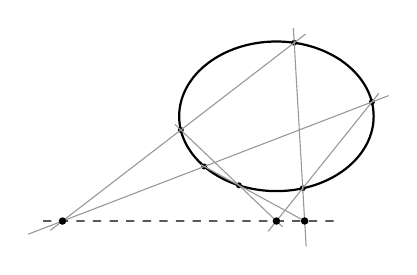
\begin{tikzpicture}[scale=0.95]
		% 二次曲线
		\draw[thick] (0,0) ellipse (1.3 and 1);
		% 六边形顶点 (反向构造: 先取 Pascal 直线 y=-1.4 与三条割线, 再反推顶点)
		\coordinate (v1) at (-0.9646,-0.671);
		\coordinate (v2) at (1.2766,0.191);
		\coordinate (v3) at (0.3519,-0.9618);
		\coordinate (v4) at (0.2380,0.9831);
		\coordinate (v5) at (-1.2780,-0.1831);
		\coordinate (v6) at (-0.5012,-0.9225);
		\foreach \i in {1,...,6} \fill (v\i) circle (0.04);
		% 六条边所在的直线 (延长至覆盖对边交点)
		\draw[gray!80, name path=L1] ($(v1)!-1.05!(v2)$) -- ($(v1)!1.1!(v2)$);
		\draw[gray!80, name path=L2] ($(v2)!-0.1!(v3)$) -- ($(v2)!1.5!(v3)$);
		\draw[gray!80, name path=L3] ($(v3)!-0.4!(v4)$) -- ($(v3)!1.1!(v4)$);
		\draw[gray!80, name path=M1] ($(v4)!-0.1!(v5)$) -- ($(v4)!2.15!(v5)$);
		\draw[gray!80, name path=M2] ($(v5)!-0.1!(v6)$) -- ($(v5)!1.75!(v6)$);
		\draw[gray!80, name path=M3] ($(v6)!-2.0!(v1)$) -- ($(v6)!1.1!(v1)$);
		% 三对对边的交点 (共线)
		\path[name intersections={of=L1 and M1, by=pa}];
		\path[name intersections={of=L2 and M2, by=pb}];
		\path[name intersections={of=L3 and M3, by=pc}];
		\fill (pa) circle (0.05);
		\fill (pb) circle (0.05);
		\fill (pc) circle (0.05);
		\draw[dashed] ($(pa)!-0.08!(pc)$) -- ($(pa)!1.15!(pc)$);
	\end{tikzpicture}
	\caption{Pascal 定理}
	\label{fig:1.6}
\end{figure}

\subsection{第 1 节习题}

\begin{compactenum}
	\item 当两个圆的交点都是复点时, 用实的术语刻画过这两个交点的直线. 证明: 它是与两圆等幂的点组成的轨迹.（点关于圆的\emph{幂}是指该点到圆的切线的切点的距离的平方.）
	\item 哪些有理函数 $p(x)/q(x)$ 在 $\PP^1$ 的无穷远点处正则? 它们在无穷远点处零点的阶是多少?
	\item 证明: 不可约三次曲线至多有一个奇异点, 且该奇异点的重数是 $2$. 若奇点是结点, 则该三次曲线射影等价于 \eqref{eq:1.2} 的曲线; 若是尖点, 则射影等价于曲线 $y^2 = x^3$.
	\item 两条非奇异二次曲线在一个公共点处的相交重数最大可能达到多少?
	\item 证明: 若基域的特征是 $p$, 则过原点的每条直线都是曲线 $y = x^{p+1}$ 的切线. 证明: 在特征 $0$ 的域上, 过一给定点且与给定不可约曲线相切的直线至多有有限多条.
	\item 证明: $n$ 次不可约曲线的两个奇异点的重数之和至多是 $n$, 而任意 $5$ 个点的重数之和至多是 $2n$.
	\item 证明: 对不可约曲线上任意两个不同的点, 存在一个在这两点都正则的有理函数, 它在其中一个点取值 $0$, 在另一个点取值 $1$.
	\item 证明: 对不可约曲线上任意非奇异点 $P_1, \ldots, P_r$ 与任意非负整数 $m_1, \ldots, m_r \ge 0$, 存在一个在这些点都正则的有理函数, 且它在 $P_i$ 处有重数恰为 $m_i$ 的零点.
	\item 三次曲线 $x_0^3 + x_1^3 + x_2^3 + m\, x_0 x_1 x_2 = 0$（$\PP^2$ 中）对哪些 $m$ 值是非奇异的? 求出它的拐点.
	\item 求曲线 \eqref{eq:1.2} 的全部自同构.
	\item 证明: 在射影直线与 $\PP^2$ 中的二次曲线上, 处处正则的有理函数必是常数.
	\item 对六边形有若干对顶点重合从而连接它们的直线变为切线的情形, 给出 Pascal 定理的解释.
\end{compactenum}

\section{仿射空间中的闭子集}

以下我们固定一个代数闭域 $k$, 称之为\emph{基域}.

\subsection{闭子集的定义}

在代数几何发展的不同阶段, 关于基本研究对象, 即关于什么才是代数簇的``自然定义''这一问题, 有过不同的观点; 被认为最基础的对象先后是射影簇或拟投影簇, 抽象代数簇, 概形或代数空间.

本书以逐步提高的一般性来展开代数几何. 前几章所考虑的最一般概念, 亦即涵盖书中所研究全部代数簇的概念, 是拟投影簇; 在最后几章中, 这个角色将由概形担任. 现在我们定义一类代数簇, 它在所有后续定义中起奠基作用. 由于``簇''一词要留给更一般的概念, 这里我们换一个说法.

我们把域 $k$ 上的 $n$ 维仿射空间记作 $\A^n$, 其点形如 $\alpha = (\alpha_1, \ldots, \alpha_n)$, $\alpha_i \in k$.

\begin{definition}[闭子集]\label{def:closed-subset}
	$\A^n$ 的\emph{闭子集}\index{biziji@闭子集}是指这样的子集 $X \subset \A^n$: 它由系数取自 $k$ 的有限多个多项式的全部公共零点组成. 为简便起见, 有时简称闭集.
\end{definition}

今后用 $F(T)$ 表示 $n$ 元多项式, $T$ 代表变量组 $T_1, \ldots, T_n$. 若闭集 $X$ 由多项式 $F_1(T), \ldots, F_m(T)$ 的全部公共零点组成, 则称 $F_1(T) = \cdots = F_m(T) = 0$ 为 $X$ 的方程组.

由无穷方程组 $F_\alpha(T) = 0$ 定义的集合 $X$ 也是闭集. 事实上, 诸 $F_\alpha(T)$ 在多项式环 $k[T_1, \ldots, T_n]$ 中生成的理想 $\mathfrak A$ 是有限生成的（Hilbert 基定理, 见 Atiyah--Macdonald \cite[定理 7.5]{atiyah-macdonald1969}）, 设 $\mathfrak A = (G_1, \ldots, G_m)$; 容易验证 $X$ 由方程组 $G_1 = \cdots = G_m = 0$ 定义.

由此, 任意多个闭集之交是闭集. 事实上, 若诸 $X_\alpha$ 是闭集, 要得到定义 $X = \bigcap_\alpha X_\alpha$ 的方程组, 只需把定义各个 $X_\alpha$ 的方程组并在一起.

有限多个闭集之并仍是闭集. 显然只需对两个集合验证: 设 $X = X_1 \cup X_2$, 其中 $X_1$ 由方程组 $F_i(T) = 0$（$i = 1, \ldots, m$）定义, $X_2$ 由 $G_j(T) = 0$（$j = 1, \ldots, l$）定义, 那么容易验证 $X$ 由方程组 $F_i(T)\, G_j(T) = 0$（$i = 1, \ldots, m$; $j = 1, \ldots, l$）定义.

设 $X \subset \A^n$ 是仿射空间中的闭子集. 若 $X \setminus U$ 是闭集, 就称子集 $U \subset X$ 为\emph{开集}; 包含点 $x$ 的任何开集 $U$ 都称为 $x$ 的一个邻域.

$X$ 中包含给定子集 $M \subset X$ 的所有闭子集之交是闭集, 称为 $M$ 的闭包, 记作 $\overline{M}$. 若 $\overline{M} = X$, 则称 $M$ 在 $X$ 中稠密; 这意味着 $M$ 不含于任何真闭子集 $Y \subsetneq X$ 之中.

\begin{example}\label{exam:An-closed}
	整个仿射空间 $\A^n$ 是闭集: 它由空的方程组定义, 或者由方程 $0 = 0$ 定义.
\end{example}

\begin{example}\label{exam:A1-minus-0}
	$\A^1$ 中由除 $0$ 以外的全部点组成的子集 $X$ 不是闭集: 在所有 $T \ne 0$ 处都取零值的多项式 $F(T)$ 必恒为零.
\end{example}

\begin{example}\label{exam:closed-in-A1}
	我们来确定 $\A^1$ 中所有的闭子集 $X$. 这样的集合由一元方程组 $F_1(T) = \cdots = F_m(T) = 0$ 给出. 若所有 $F_i$ 恒为零, 则 $X = \A^1$; 若诸 $F_i$ 没有公因子, 则它们没有公共根, $X$ 不含任何点; 若诸 $F_i$ 的最高公因子是 $D(T)$, 则 $D(T) = (T - \alpha_1) \cdots (T - \alpha_n)$, 而 $X$ 由有限多个点 $T = \alpha_1, \ldots, \alpha_n$ 组成.
\end{example}

\begin{example}\label{exam:closed-in-A2}
	我们来确定 $\A^2$ 中所有的闭子集 $X$. 闭集由方程组
	\begin{equation}
		\label{eq:1.17}
		F_1(T) = \cdots = F_m(T) = 0
	\end{equation}
	给出, 此时 $T = (T_1, T_2)$. 若所有 $F_i$ 恒为零, 则 $X = \A^2$; 设不是这种情形. 若多项式 $F_1, \ldots, F_m$ 没有公因子, 则由 §1.1 的引理~\ref{lem:finite-solutions}, 方程组 \eqref{eq:1.17} 只有有限多个解（也可能是空集）.

	最后, 设诸 $F_i(T)$ 的最高公因子是 $D(T)$, 于是 $F_i(T) = D(T)\, G_i(T)$, 而诸 $G_i(T)$ 没有公因子. 此时有 $X = X_1 \cup X_2$, 其中 $X_1$ 由 $G_1(T) = \cdots = G_m(T) = 0$ 给出, $X_2$ 由单个方程 $D(T) = 0$ 给出. 如例~\ref{exam:closed-in-A1} 所见, $X_1$ 是有限集; 而由单个方程定义的 $\A^2$ 中的闭集正是代数平面曲线. 于是 $\A^2$ 中的闭集 $X$ 或者由有限多个点组成（可以是空集）, 或者是一条代数平面曲线与有限多个点之并, 或者是整个 $\A^2$.
\end{example}

\begin{example}\label{exam:product-closed}
	设 $\alpha \in \A^r$ 是坐标为 $(\alpha_1, \ldots, \alpha_r)$ 的点, $\beta \in \A^s$ 是坐标为 $(\beta_1, \ldots, \beta_s)$ 的点, 我们把 $\alpha, \beta$ 对应到 $\A^{r+s}$ 中坐标为 $(\alpha_1, \ldots, \alpha_r, \beta_1, \ldots, \beta_s)$ 的点 $(\alpha, \beta)$. 这样, 我们把 $\A^{r+s}$ 等同于满足 $\alpha \in \A^r$, $\beta \in \A^s$ 的点对 $(\alpha, \beta)$ 的集合. 设 $X \subset \A^r$ 与 $Y \subset \A^s$ 是闭集. 由满足 $x \in X$ 与 $y \in Y$ 的点对 $(x, y) \in \A^{r+s}$ 组成的集合称为 $X$ 与 $Y$ 的积, 记作 $X \times Y$.

	它仍是闭集: 若 $X$ 由 $F_i(T) = 0$ 定义而 $Y$ 由 $G_j(U) = 0$ 定义, 则 $X \times Y \subset \A^{r+s}$ 由方程组 $F_i(T) = G_j(U) = 0$ 定义.
\end{example}

\begin{example}\label{exam:hypersurface}
	由单个方程 $F(T_1, \ldots, T_n) = 0$ 定义的集合 $X \subset \A^n$ 称为超曲面.
\end{example}

\subsection{闭子集上的正则函数}

设 $X$ 是基域 $k$ 上的仿射空间 $\A^n$ 中的闭集.

\begin{definition}[正则函数]\label{def:regular-function}
	定义在 $X$ 上且取值在 $k$ 中的函数 $f$ 称为\emph{正则}的, 如果存在系数取自 $k$ 的多项式 $F(T)$, 使得对一切 $x \in X$ 都有 $f(x) = F(x)$.
\end{definition}

对给定的函数 $f$, 多项式 $F$ 一般不是唯一确定的: 给 $F$ 加上 $X$ 的方程组中的任何一个多项式, 都不改变 $f$. 给定闭集 $X$ 上的全体正则函数构成一个环, 也构成 $k$ 上的一个代数; 加法, 乘法与用 $k$ 中元素作的数乘都像分析中那样, 通过在每点 $x \in X$ 处对函数值施行相应运算来定义. 这样得到的环记作 $k[X]$, 称为 $X$ 的\emph{坐标环}.

用 $k[T]$ 表示系数在 $k$ 中而变量为 $T_1, \ldots, T_n$ 的多项式环. 每个多项式 $F \in k[T]$ 显然给出一个函数 $f \in k[X]$, 即把 $F$ 视为 $X$ 的点集上的函数; 这样得到从 $k[T]$ 到 $k[X]$ 的一个同态. 这个同态的核由在 $X$ 的每一点 $x$ 处取值为 $0$ 的全体多项式 $F \in k[T]$ 组成; 与任何环同态的核一样, 它是 $k[T]$ 的理想, 称为闭集 $X$ 的\emph{理想}, 记作 $\mathfrak A_X$. 显然
\[
	k[X] = k[T] / \mathfrak A_X.
\]
因此 $k[X]$ 由理想 $\mathfrak A_X \subset k[T]$ 确定.

\begin{example}\label{exam:point-ring}
	若 $X$ 是一个点, 则 $k[X] = k$.
\end{example}

\begin{example}\label{exam:An-ring}
	若 $X = \A^n$, 则 $\mathfrak A_X = 0$, 且 $k[X] = k[T]$.
\end{example}

\begin{example}\label{exam:hyperbola-ring}
	设 $X \subset \A^2$ 由方程 $T_1 T_2 = 1$ 给出, 则 $k[X] = k[T_1, T_1^{-1}]$, 它由形如 $G(T_1)/T_1^n$ 的 $T_1$ 的有理函数组成, 其中 $G(T_1)$ 是多项式而 $n \ge 0$.
\end{example}

\begin{example}\label{exam:tensor-product-ring}
	我们证明, 对任意闭集 $X$ 与 $Y$ 有 $k[X \times Y] = k[X] \otimes_k k[Y]$. 定义同态 $\varphi: k[X] \otimes_k k[Y] \to k[X \times Y]$ 为
	\[
		\varphi\Bigl( \sum_i f_i \otimes g_i \Bigr)(x, y) = \sum_i f_i(x)\, g_i(y).
	\]
	右端显然是 $X \times Y$ 上的正则函数; 并且 $\varphi$ 显然是满射, 因为（用例~\ref{exam:product-closed} 的记号）函数 $\alpha_i$ 与 $\beta_j$ 都含于 $\varphi$ 的像中, 而它们生成 $k[X \times Y]$.

	为证 $\varphi$ 是单射, 只需验证: 若 $\{f_i\}$ 在 $k[X]$ 中线性无关且 $\{g_j\}$ 在 $k[Y]$ 中线性无关, 则 $\{f_i \otimes g_j\}$ 在 $k[X \times Y]$ 中线性无关. 而等式 $\sum_{i,j} c_{ij}\, f_i(x)\, g_j(y) = 0$ 蕴含对每个固定的 $y$ 与每个 $i$ 有 $\sum_j c_{ij}\, g_j(y) = 0$, 从而 $c_{ij} = 0$.
\end{example}

由于 $k[X]$ 是多项式环 $k[T]$ 的同态像, 它满足 Hilbert 基定理: $k[X]$ 的任何理想都有限生成. 它还满足 Nullstellensatz 的如下类似物（原书附录命题 A.9）: 若函数 $f \in k[X]$ 在使 $g_1, \ldots, g_m$ 都为零的每一点 $x \in X$ 处为零, 则存在 $r > 0$ 使 $f^r \in (g_1, \ldots, g_m)$.

事实上, 设 $f$ 由多项式 $F(T)$ 给出, $g_i$ 由多项式 $G_i(T)$ 给出, 并设 $F_j = 0$（$j = 1, \ldots, l$）是 $X$ 的方程组. 那么 $F(T)$ 在使多项式 $G_1, \ldots, G_m, F_1, \ldots, F_l$ 全为零的每一点 $\alpha \in \A^n$ 处为零: 因为 $F_j(\alpha) = 0$ 意味着 $\alpha \in X$, 而由假设便得 $F(\alpha) = 0$. 在多项式环上应用 Nullstellensatz, 推出对某个 $r > 0$ 有 $F^r \in (G_1, \ldots, G_m, F_1, \ldots, F_l)$, 于是在 $k[X]$ 中 $f^r \in (g_1, \ldots, g_m)$.

闭集 $X$ 的理想 $\mathfrak A_X$ 与它的定义方程组 $F_1 = \cdots = F_m = 0$ 之间有什么关系? 显然, 按 $\mathfrak A_X$ 的定义有 $F_i \in \mathfrak A_X$, 故 $(F_1, \ldots, F_m) \subset \mathfrak A_X$; 但 $(F_1, \ldots, F_m) = \mathfrak A_X$ 并不总成立. 例如, 若 $X \subset \A^1$ 由方程 $T^2$ 定义, 则它恰由点 $T = 0$ 组成, 于是 $\mathfrak A_X$ 由所有不含常数项的多项式组成, 即 $\mathfrak A_X = (T)$, 而 $(F_1, \ldots, F_m) = (T^2)$.

不过, 我们总可以选取定义同一闭集 $X$ 的方程组 $G_1 = \cdots = G_l = 0$, 使得 $\mathfrak A_X = (G_1, \ldots, G_l)$. 为此只需回忆, $k[T]$ 的任何理想都有限生成: 取理想 $\mathfrak A_X$ 的一组生成元 $G_1, \ldots, G_l$, 即 $\mathfrak A_X = (G_1, \ldots, G_l)$, 则方程组 $G_1 = \cdots = G_l = 0$ 显然定义同一集合 $X$ 且具有所需的性质. 有时甚至更方便的是把闭集视为由无穷方程组 $F = 0$（$F$ 取遍 $\mathfrak A_X$ 中的多项式）定义: 若 $(F_1, \ldots, F_m) = \mathfrak A_X$, 那么这些方程都是 $F_1 = \cdots = F_m = 0$ 的推论.

闭集之间的包含关系常反映在它们的理想上. 例如, 对 $\A^n$ 中的闭集 $X$ 与 $Y$, 有 $X \supset Y$ 当且仅当 $\mathfrak A_X \subset \mathfrak A_Y$. 由此, 对含于 $X$ 中的任一闭子集 $Y$, 可以对应 $k[X]$ 中的理想 $\mathfrak a_Y$, 它由多项式 $F \in \mathfrak A_Y$ 在同态 $k[T] \to k[X]$ 下的像组成. 反之, $k[X]$ 的任一理想 $\mathfrak a$ 确定 $k[T]$ 中的一个理想 $\mathfrak A$, 由 $\mathfrak a$ 中元素在同态 $k[T] \to k[X]$ 下的全体原像组成; 显然 $\mathfrak A \supset \mathfrak A_X$, 而方程组 $F = 0$（$F$ 取遍 $\mathfrak A$）定义一个闭集 $Y \subset X$.

由 Nullstellensatz, $Y$ 是空集当且仅当 $\mathfrak a_Y = k[X]$. 理想 $\mathfrak a_Y \subset k[X]$ 也可以刻画为在子集 $Y$ 的所有点处取零的全体函数 $f \in k[X]$.

特别地, 每个点 $x \in X$ 本身是闭子集, 从而定义 $k[X]$ 中的一个理想 $\mathfrak m_x$. 按定义, 这个理想是把 $f \in k[X]$ 映到其值 $f(x)$ 的同态 $k[X] \to k$ 的核. 既然 $k[X]/\mathfrak m_x = k$ 是域, 理想 $\mathfrak m_x$ 是极大的. 反之, 每个极大理想 $\mathfrak m \subset k[X]$ 都以这种方式对应于某个点 $x \in X$: 它定义一个闭子集 $Y \subset X$; 对任一点 $y \in Y$ 有 $\mathfrak m_y \supset \mathfrak m$, 于是由 $\mathfrak m$ 的极大性得 $\mathfrak m_y = \mathfrak m$.

对 $u \in k[X]$, 使 $u(x) = 0$ 的点 $x \in X$ 组成的集合是闭集, 记作 $V(u)$, 称为 $X$ 中的超曲面.

\subsection{正则映射}

设 $X \subset \A^n$ 与 $Y \subset \A^m$ 是闭子集.

\begin{definition}[正则映射]\label{def:regular-map-affine}
	映射 $f: X \to Y$ 称为\emph{正则}的, 如果存在 $X$ 上的 $m$ 个正则函数 $f_1, \ldots, f_m$, 使得对一切 $x \in X$ 都有 $f(x) = (f_1(x), \ldots, f_m(x))$.
\end{definition}

于是, 任何正则映射 $f: X \to \A^m$ 由 $m$ 个函数 $f_1, \ldots, f_m \in k[X]$ 给出; 而要知道它映入闭子集 $Y \subset \A^m$, 显然只需验证 $f_1, \ldots, f_m$ 作为 $k[X]$ 的元素满足 $Y$ 的方程, 即对一切 $G \in \mathfrak A_Y$ 有 $G(f_1, \ldots, f_m) = 0 \in k[X]$.

\begin{example}\label{exam:function-as-map}
	$X$ 上的正则函数恰好就是到 $\A^1$ 的正则映射.
\end{example}

\begin{example}\label{exam:linear-map}
	线性映射 $\A^n \to \A^m$ 是正则映射.
\end{example}

\begin{example}\label{exam:hyperbola-projection}
	投影映射 $(x, y) \mapsto x$ 给出由方程 $xy = 1$ 定义的曲线到 $\A^1$ 的一个正则映射.
\end{example}

\begin{example}\label{exam:local-invert}
	前例可以推广: 设 $X \subset \A^n$ 是闭子集, $F$ 是 $X$ 上的正则函数. 考虑由方程 $T_{n+1}\, F(T_1, \ldots, T_n) = 1$ 定义的子集 $X' \subset X \times \A^1$. 投影 $\varphi(x_1, \ldots, x_{n+1}) = (x_1, \ldots, x_n)$ 给出正则映射 $\varphi: X' \to X$.
\end{example}

\begin{example}\label{exam:cusp-map}
	映射 $f(t) = (t^2, t^3)$ 是直线 $\A^1$ 到由 $y^2 = x^3$ 给出的曲线的正则映射.
\end{example}

\begin{example}[{$\F_p$ 上簇的 zeta 函数}]\label{exam:zeta}
	我们给出一个对数论十分重要的例子. 设闭子集 $X \subset \A^n$ 的方程 $F_i(T)$ 的系数都属于含 $p$ 个元素的域 $\F_p$, 其中 $p$ 是素数.

	如 §1.1 所述, $X$ 的坐标属于 $\F_p$ 的点对应于同余方程组 $F_i(T) \equiv 0 \pmod{p}$ 的解. 考虑由
	\[
		\varphi(\alpha_1, \ldots, \alpha_n) = (\alpha_1^p, \ldots, \alpha_n^p)
	\]
	定义的映射 $\varphi: \A^n \to \A^n$. 它显然是正则映射. 要紧的是, 它把 $X \subset \A^n$ 映到自身: 若 $\alpha \in X$, 即 $F_i(\alpha) = 0$, 则因 $F_i(T) \in \F_p[T]$, 由特征 $p$ 域的性质得 $F_i(\alpha_1^p, \ldots, \alpha_n^p) = \bigl( F_i(\alpha_1, \ldots, \alpha_n) \bigr)^p = 0$. 这样得到的映射 $\varphi: X \to X$ 称为 Frobenius 映射\index{Frobenius yingshe@Frobenius 映射}. 其意义在于: 在 $X$ 的所有点中, 坐标属于 $\F_p$ 的点恰好被刻画为 $\varphi$ 的不动点, 因为方程 $\alpha_i^p = \alpha_i$ 的解恰是 $\F_p$ 的全部元素.

	完全同样地, 含 $p^r$ 个元素的域 $\F_{p^r}$ 的元素 $\alpha$ 被刻画为方程 $\alpha^{p^r} = \alpha$ 的解, 于是 $X$ 的坐标属于 $\F_{p^r}$ 的点恰是映射 $\varphi^r$ 的不动点. 对每个 $r$, 用 $\nu_r$ 表示 $X$ 的坐标属于 $\F_{p^r}$ 的点数. 为对数集 $\{\nu_r\}$ 有个总览, 考虑生成函数
	\[
		P_X(t) = \sum_{r=1}^{\infty} \nu_r\, t^r.
	\]
	一个深刻的普遍定理断言: 这个函数总是 $t$ 的有理函数（相当初等的证明见 Koblitz \cite[第 V 章]{koblitz1984}）. 这样, $P_X(t)$ 便以有限的形式表达了无穷数列 $\nu_r$.

	与闭集 $X$ 相伴的函数 $P_X(t)$ 具有与 Riemann zeta 函数类似的一些性质. 为表述它们, 注意: 若 $x \in X$ 是坐标属于 $\F_{p^r}$ 且生成该域的点, 则 $X$ 包含所有的点 $\varphi^i(x)$（$i = 1, \ldots, r$）, 且这些点两两不同. 我们称这种形式的集合 $\xi = \{\varphi^i(x)\}$ 为一个\emph{循环}, 其点数 $r$ 称为 $\xi$ 的次数, 记作 $\deg \xi$.

	现在可把 $X$ 的坐标属于 $\F_{p^r}$ 的全部 $\nu_r$ 个点按循环分组. 这些点中任一点的坐标生成某个子域 $\F_{p^d} \subset \F_{p^r}$, 且已知 $d \mid r$（例如见 van der Waerden \cite[第 6.7 节例 6.23]{vdw1991}）. 于是得到公式
	\[
		\nu_r = \sum_{d \mid r} d\, \mu_d,
	\]
	其中 $\mu_d$ 是次数为 $d$ 的循环的个数, 从而
	\begin{equation}
		\label{eq:1.18}
		P_X(t) = \sum_{r=1}^{\infty} \sum_{d \mid r} d\, \mu_d\, t^r = \sum_{d=1}^{\infty} d\, \mu_d \sum_{m=1}^{\infty} t^{md} = \sum_{d=1}^{\infty} \mu_d\, \frac{d\, t^d}{1 - t^d}.
	\end{equation}

	我们引进函数
	\begin{equation}
		\label{eq:1.19}
		Z_X(t) = \prod_{\xi} \frac{1}{1 - t^{\deg \xi}},
	\end{equation}
	其中乘积取遍全部循环 $\xi$. 这时公式 \eqref{eq:1.18} 显然可改写为
	\[
		P_X(t) = \frac{Z'_X(t)}{Z_X(t)}\, t.
	\]
	等式 \eqref{eq:1.19} 与 Riemann zeta 函数的 Euler 乘积类似. 为强调这一类比, 令 $N(\xi) = p^{\deg \xi}$, $t = p^{-s}$, 则 \eqref{eq:1.19} 取得形式
	\[
		Z_X(t) = \zeta_X(s) = \prod_{\xi} \frac{1}{1 - N(\xi)^{-s}}.
	\]
	函数 $Z_X(t)$（或 $\zeta_X(s)$）称为 $X$ 的 zeta 函数.
\end{example}

现在弄清正则映射如何作用于闭集的正则函数环. 先就集合之间任意的映射作一点说明. 设 $f: X \to Y$ 是从集合 $X$ 到集合 $Y$ 的映射, 那么对 $Y$ 上每个（取值于某个集合 $Z$ 的）函数 $u$, 令 $v(x) = u(f(x))$ 便得到 $X$ 上的函数 $v$; 显然 $v: X \to Z$ 是 $f: X \to Y$ 与 $u: Y \to Z$ 的复合. 记 $v = f^*(u)$, 称之为 $u$ 的拉回; 这样得到从 $Y$ 上的函数到 $X$ 上的函数的映射 $f^*$.

现在设 $f: X \to Y$ 是正则映射, 则 $f^*$ 把 $Y$ 上的正则函数送到 $X$ 上的正则函数. 事实上, 若 $u$ 由多项式函数 $G(T_1, \ldots, T_n)$ 给出, 而 $f$ 由多项式 $F_1, \ldots, F_m$ 给出, 则 $v = f^*(u)$ 只需把 $G$ 中的 $T_i$ 换成 $F_i$ 便得, 故 $v$ 由多项式 $G(F_1, \ldots, F_m)$ 给出.

而且, 正则映射恰好可以刻画为把正则函数送到正则函数的映射. 事实上, 设闭集间的映射 $f: X \to Y$ 具有性质: 对 $Y$ 上的每个正则函数 $u$, $X$ 上的函数 $f^*(u)$ 仍是正则的. 那么这特别适用于由 $Y$ 上的坐标 $T_i$（$i = 1, \ldots, m$）定义的函数 $t_i$, 于是诸函数 $f^*(t_i)$ 在 $X$ 上正则; 而这恰好说明 $f$ 是正则映射.

我们已见, 若 $f$ 正则, 则函数的拉回给出映射 $f^*: k[Y] \to k[X]$; 由 $f^*$ 的定义容易推出它是 $k$-代数同态. 我们证明, 反之, 每个代数同态 $\varphi: k[Y] \to k[X]$ 都形如 $\varphi = f^*$, 其中 $f: X \to Y$ 是某个正则映射. 设 $t_1, \ldots, t_m$ 是 $Y$ 的外围空间 $\A^m$ 的坐标, 视为 $Y$ 上的函数. 显然 $t_i \in k[Y]$, 故 $\varphi(t_i) \in k[X]$. 记 $\varphi(t_i) = s_i$, 考虑由公式 $f(x) = (s_1(x), \ldots, s_m(x))$ 给出的映射 $f$; 这当然是正则映射.

	我们证明 $f(X) \subset Y$. 事实上, 若 $H \in \mathfrak A_Y$, 则 $H(t_1, \ldots, t_m) = 0$ 在 $k[Y]$ 中成立, 于是在 $X$ 上有 $\varphi(H) = 0$. 设 $x \in X$, 则 $H(f(x)) = \varphi(H)(x) = 0$, 因此 $f(x) \in Y$.

\begin{definition}[同构]\label{def:isomorphism}
	闭集之间的正则映射 $f: X \to Y$ 称为\emph{同构}, 如果它有逆, 即存在正则映射 $g: Y \to X$ 使得 $f \circ g = 1$ 且 $g \circ f = 1$. 这时称 $X$ 与 $Y$ 同构.
\end{definition}

同构显然是一一对应. 由上述内容可知, 若 $f$ 是同构, 则 $f^*: k[Y] \to k[X]$ 是代数同构; 反之亦易见成立. 换言之, 闭集同构当且仅当它们的正则函数环在 $k$ 上同构.

刚才证明的事实表明, $X \mapsto k[X]$ 给出仿射空间闭子集（连同其间的正则映射）的范畴与 $k$ 上交换代数范畴的某个子范畴（连同代数同态）之间的等价. 这个子范畴是什么样的, 即哪些代数形如 $k[X]$?

\begin{theorem}\label{thm:coordinate-ring-char}
	域 $k$ 上的代数 $A$ 同构于某个闭子集 $X$ 的坐标环 $k[X]$, 当且仅当 $A$ 没有幂零元（即对 $f \in A$, 由 $f^m = 0$ 可推出 $f = 0$）, 并且作为 $k$ 上的代数是有限生成的.
\end{theorem}

\begin{proof}
	这些条件显然都是必要的. 设代数 $A$ 由有限多个元素 $t_1, \ldots, t_n$ 生成, 则 $A \cong k[T_1, \ldots, T_n]/\mathfrak A$, 其中 $\mathfrak A$ 是多项式环 $k[T_1, \ldots, T_n]$ 的理想. 设 $\mathfrak A = (F_1, \ldots, F_m)$, 考虑由方程 $F_1 = \cdots = F_m = 0$ 定义的闭集 $X \subset \A^n$; 我们证明 $\mathfrak A_X = \mathfrak A$, 由此便得 $k[X] \cong k[T_1, \ldots, T_n]/\mathfrak A \cong A$.

	若 $F \in \mathfrak A_X$, 则由 Nullstellensatz, 对某个 $r > 0$ 有 $F^r \in \mathfrak A$. 既然 $A$ 没有幂零元, 也有 $F \in \mathfrak A$. 于是 $\mathfrak A_X \subset \mathfrak A$; 而显然 $\mathfrak A \subset \mathfrak A_X$, 故 $\mathfrak A_X = \mathfrak A$. 定理证毕.
\end{proof}

\begin{example}\label{exam:parabola-iso}
	由方程 $y = x^k$ 定义的广义抛物线同构于直线, 且映射 $f(x, y) = x$ 与 $g(t) = (t, t^k)$ 给出一个同构.
\end{example}

\begin{example}\label{exam:hyperbola-not-iso}
	双曲线 $xy = 1$ 到 $x$ 轴的投影 $f(x, y) = x$ 不是同构, 因为这个映射不是一一对应: 双曲线不含使 $f(x, y) = 0$ 的点 $(x, y)$. 亦比较本节习题 4.
\end{example}

\begin{example}\label{exam:cusp-not-iso}
	直线到曲线 $y^2 = x^3$ 的映射 $f(t) = (t^2, t^3)$（例~\ref{exam:cusp-map}）容易看出是一一对应. 然而它不是同构: 逆映射形如 $g(x, y) = y/x$, 而函数 $y/x$ 在原点处不正则.（见本节习题 5.）
\end{example}

\begin{example}\label{exam:diagonal}
	设 $X, Y \subset \A^n$ 是闭集. 如例~\ref{exam:product-closed} 那样考虑 $X \times Y \subset \A^{2n}$, 以及由方程 $t_1 = u_1, \ldots, t_n = u_n$ 定义的线性子空间 $\Delta \subset \A^{2n}$, 称为对角线. 把每点 $z \in X \cap Y$ 映为 $\varphi(z) = (z, z) \in \A^{2n}$, 得到的显然是 $X \times Y \cap \Delta$ 的点. 容易验证, 这样得到的映射 $\varphi: X \cap Y \to X \times Y \cap \Delta$ 是 $X \cap Y$ 到 $X \times Y \cap \Delta$ 的同构. 利用这一点, 两个闭集之交的研究总可以化为某个闭集与线性子空间之交的研究.
\end{example}

\begin{example}[商簇]\label{exam:quotient}
	设 $X$ 是闭集, $G$ 是 $X$ 的自同构组成的有限群, 并设域 $k$ 的特征不整除 $G$ 的阶 $N$. 令 $A = k[X]$, 用 $A^G$ 表示 $G$ 在 $A$ 中的不变量子代数, 即 $A^G = \{\, f \in A \mid g^*(f) = f \text{ 对一切 } g \in G \,\}$. 据原书附录命题 A.6, 代数 $A^G$ 在 $k$ 上有限生成. 由定理~\ref{thm:coordinate-ring-char}, 存在闭集 $Y$ 使 $A^G \cong k[Y]$, 并存在正则映射 $\varphi: X \to Y$ 使 $\varphi^*(k[Y]) = A^G$. 集合 $Y$ 称为 $X$ 关于群 $G$ 作用的\emph{商簇}\index{shangcu@商簇}或商空间, 记作 $X/G$.

	对给定的两点 $x_1, x_2 \in X$, 存在 $g \in G$ 使 $x_2 = g(x_1)$, 当且仅当 $\varphi(x_1) = \varphi(x_2)$. 事实上, 若 $x_2 = g(x_1)$, 则对每个 $f \in k[X]^G = k[Y]$ 有 $f(x_2) = f(x_1)$, 故 $\varphi(x_1) = \varphi(x_2)$. 反之, 设对一切 $g \in G$ 都有 $x_2 \ne g(x_1)$, 则可取函数 $f \in k[X]$, 使对一切 $g \in G$ 有 $f(g(x_2)) = 1$ 且 $f(g(x_1)) = 0$; 于是对称化函数 $S(f)$（见原书附录第 4 节）是 $G$-不变的, 且满足 $S(f)(x_2) = 1$, $S(f)(x_1) = 0$, 故 $\varphi(x_2) \ne \varphi(x_1)$. 因此 $X/G$ 参数化 $G$ 作用在 $X$ 上的轨道 $\{\, g(x) \mid g \in G \,\}$.
\end{example}

今后我们主要关心闭集在同构之下不变的概念与性质. 定义集合的方程组显然不属于这类概念: 两个集合 $X$ 与 $Y$ 可以同构, 尽管它们在不同的空间 $\A^n$ 中由不同的方程组给出. 因此, 很自然地要给出闭集的一种内蕴定义, 不依赖于它在某个仿射空间中的实现; 这类定义将在第 5--6 章结合概形概念给出.

现在确定, 与正则映射 $f: X \to Y$ 相应的同态 $f^*: k[Y] \to k[X]$ 何时没有核, 亦即何时 $f^*$ 是同构嵌入 $k[Y] \hookrightarrow k[X]$. 设 $u \in k[Y]$, 来看何时 $f^*(u) = 0$. 这意味着对一切 $x \in X$ 有 $u(f(x)) = 0$; 换言之, $u$ 在 $X$ 的像 $f(X)$ 的所有点上为零.

使 $u(y) = 0$ 的点 $y \in Y$ 显然组成闭集, 故若它包含 $f(X)$, 也就包含闭包 $\overline{f(X)}$. 把同样的论证倒回去, 便知 $f^*(u) = 0$ 当且仅当 $u$ 在 $\overline{f(X)}$ 上为零, 亦即等价地 $u \in \mathfrak a_{\overline{f(X)}}$. 特别地, $f^*$ 的核为零当且仅当 $\overline{f(X)} = Y$, 即 $f(X)$ 在 $Y$ 中稠密. 当 $f(X) = Y$ 时当然如此, 但也存在 $f(X) \ne Y$ 而 $\overline{f(X)} = Y$ 的情形（见例~\ref{exam:hyperbola-projection}）.

今后我们主要研究射影空间中的代数簇. 但仿射空间的闭子集也有一种风味独特的几何, 往往相当不平凡. 作为例子, 我们给出 Abhyankar 与 Moh 的下述定理.

\begin{theorem}[Abhyankar--Moh]\label{thm:abhyankar-moh}
	曲线 $X \subset \A^2$ 同构于 $\A^1$, 当且仅当存在 $\A^2$ 的自同构把 $X$ 变为一条直线.（这里自同构指 $\A^2$ 到自身的同构.）
\end{theorem}

平面自同构群 $\operatorname{Aut} \A^2$ 是一个非常有趣的对象. 某些自同构的例子很容易构造: 仿射线性映射, 以及形如
\begin{equation}
	\label{eq:1.20}
	x' = \alpha x, \quad y' = \beta y + f(x)
\end{equation}
的映射, 其中 $\alpha, \beta \ne 0$ 是常数而 $f$ 是多项式. 已知整个群 $\operatorname{Aut} \A^2$ 由这些自同构生成. 而且, 把元素 $g \in \operatorname{Aut} \A^2$ 表为仿射线性映射与 \eqref{eq:1.20} 型映射之积的表达式几乎是唯一的: 这两类映射在 $\operatorname{Aut} \A^2$ 中满足的关系, 只有由两类有公共部分（即 $f$ 取线性多项式时的 \eqref{eq:1.20} 型映射）所表达的那些. 用抽象群论的语言说, $\operatorname{Aut} \A^2$ 是两个子群（\eqref{eq:1.20} 型映射组成的子群与仿射映射组成的子群）沿其公共子群的自由积（见 Kurosh \cite[第 IX 章第 35 节及例 10]{kurosh1960}）.

与 $\A^2$ 自同构有关的一个著名未解决问题是 Jacobi 猜想. 它断言: 若基域 $k$ 的特征为 $0$, 则由
\[
	x' = f(x, y), \qquad y' = g(x, y) \qquad (f, g \in k[x,y])
\]
给出的映射是 $\A^2$ 的自同构, 当且仅当 Jacobi 行列式 $\dfrac{\partial(f, g)}{\partial(x, y)}$ 是非零常数. 目前, 这猜想已在 $f$ 与 $g$ 的次数不太大（约 $100$ 阶）的情形下被证明. 对 $n$ 维仿射空间 $\A^n$ 有类似的猜想.

\subsection{第 2 节习题}

\begin{compactenum}
	\item $\A^2$ 中的集合 $X$ 由方程 $f:\ x^2 + y^2 = 1$ 与 $g:\ x = 1$ 定义. 求理想 $\mathfrak A_X$. 是否有 $\mathfrak A_X = (f, g)$?
	\item 设 $X \subset \A^2$ 是由 $y^2 = x^3$ 定义的代数平面曲线. 证明: $k[X]$ 的每个元素都可以唯一地写成 $P(x) + Q(x)\, y$ 的形式, 其中 $P(x), Q(x)$ 是多项式.
	\item 设 $X$ 是习题 2 的曲线, $f(t) = (t^2, t^3)$ 是正则映射 $\A^1 \to X$. 证明 $f$ 不是同构.（提示: 利用习题 2 的结果, 尝试把 $f$ 的逆构造成正则映射.）
	\item 设 $X$ 是由方程 $y^2 = x^2 + x^3$ 定义的曲线, $f: \A^1 \to X$ 由 $f(t) = (t^2 - 1,\ t(t^2 - 1))$ 定义. 证明相应的同态 $f^*$ 把 $k[X]$ 同构地映到 $k[t]$ 中由满足 $g(1) = g(-1)$ 的多项式 $g(t)$ 组成的子环.（设 $\operatorname{char} k \ne 2$.）
	\item 证明: 由 $xy = 1$ 定义的双曲线与直线 $\A^1$ 不同构.
	\item 考虑由 $f(x, y) = (x, xy)$ 定义的正则映射 $f: \A^2 \to \A^2$. 求 $f(\A^2)$; 它在 $\A^2$ 中是开集吗? 稠密吗? 是闭集吗?
	\item 对由 $f(x, y, z) = (x, xy, xyz)$ 定义的映射 $f: \A^3 \to \A^3$, 回答与习题 6 相同的问题.
	\item 闭集 $X$ 到自身的同构 $f: X \to X$ 称为\emph{自同构}. 证明: 直线 $\A^1$ 的全部自同构都形如 $f(x) = ax + b$（$a \ne 0$）.
	\item 证明 $f(x, y) = (\alpha x, \beta y + P(x))$ 是 $\A^2$ 的自同构, 其中 $\alpha, \beta \in k$ 非零, $P(x)$ 是多项式. 证明这类映射构成一个群 $B$.
	\item 证明: 若 $f(x_1, \ldots, x_n) = (P_1(x_1, \ldots, x_n), \ldots, P_n(x_1, \ldots, x_n))$ 是 $\A^n$ 的自同构, 则 Jacobi 行列式 $J(f) = \det \bigl| \partial P_i / \partial x_j \bigr| \in k$. 证明 $f \mapsto J(f)$ 是从 $\A^n$ 的自同构群到 $k$ 中非零元素乘法群的同态.
	\item 设 $X$ 由两个点组成. 证明: 坐标环 $k[X]$ 同构于两个 $k$ 的直和.
	\item 设 $f: X \to Y$ 是正则映射. 由全部形如 $(x, f(x))$ 的点组成的子集 $\Gamma_f \subset X \times Y$ 称为 $f$ 的\emph{图}. 证明: (a) $\Gamma_f \subset X \times Y$ 是闭子集; (b) $\Gamma_f$ 同构于 $X$.
	\item 由 $p_Y(x, y) = y$ 定义的映射 $p_Y: X \times Y \to Y$ 称为到 $Y$ 的投影或第二投影. 证明: 若 $Z \subset X$ 且 $f: X \to Y$ 是正则映射, 则 $f(Z) = p_Y\bigl( (Z \times Y) \cap \Gamma_f \bigr)$, 其中 $\Gamma_f$ 是 $f$ 的图, 而 $Z \times Y \subset X \times Y$ 是满足 $z \in Z$ 的点 $(z, y)$ 的集合.
	\item 证明: 对任何正则映射 $f: X \to Y$, 存在正则映射 $g: X \to X \times Y$, 它是 $X$ 到 $X \times Y$ 的某个闭子集的同构, 且满足 $f = p_Y \circ g$. 换言之, 任何映射都是嵌入与投影的复合.
	\item 证明: 若 $X = \bigcup U_\alpha$ 是闭集 $X$ 的任意一个开覆盖, 则存在有限多个 $U_{\alpha_1}, \ldots, U_{\alpha_r}$ 使得 $X = U_{\alpha_1} \cup \cdots \cup U_{\alpha_r}$.
	\item 证明 Frobenius 映射 $\varphi$（例~\ref{exam:zeta}）是一一对应. 它是同构吗, 例如取 $X = \A^1$ 时?
	\item 对 $X = \A^n$ 求 zeta 函数 $Z_X(t)$.
	\item 设 $X$ 是 $\A^2$ 中一条非奇异二次曲线, 确定 $Z_X(t)$.
\end{compactenum}

\section{有理函数}

\subsection{不可约代数子集}

在 §1.1 我们引进了平面上不可约代数曲线的概念. 现在把它推广为一般情形的相应概念.

\begin{definition}[不可约闭集]\label{def:irreducible-set}
	闭代数集 $X$ 称为\emph{可约}的, 如果存在真闭子集 $X_1, X_2 \subsetneq X$ 使 $X = X_1 \cup X_2$; 否则称 $X$ \emph{不可约}.
\end{definition}

\begin{theorem}\label{thm:finite-union-irreducible}
	任何闭集 $X$ 都是有限多个不可约闭集之并.
\end{theorem}

\begin{proof}
	设定理对某个集合 $X$ 不成立. 那么 $X$ 可约, $X = X_1 \cup X'_1$, 而定理对 $X_1$ 或 $X'_1$ 之一必不成立; 设对 $X_1$ 不成立. 那么 $X_1$ 又可约, 它又由两个闭集组成, 其中一个是可约的. 这样便得到闭子集的严格递降无穷链 $X \supsetneq X_1 \supsetneq X_2 \supsetneq \cdots$. 我们证明这样的链不可能存在. 事实上, 与诸 $X_i$ 相应的理想将构成严格递增链 $\mathfrak A_X \subsetneq \mathfrak A_{X_1} \subsetneq \mathfrak A_{X_2} \subsetneq \cdots$, 而多项式环的每个理想都有有限基, 故理想的递增链必终止, 矛盾. 定理证毕.
\end{proof}

若 $X = \bigcup X_i$ 是 $X$ 表示为有限多个不可约闭集之并的一个表达式, 且对某对 $i \ne j$ 有 $X_i \subset X_j$, 则可从表达式中删去 $X_i$. 如此重复若干次, 便得到一个表示 $X = \bigcup X_i$, 其中对一切 $i \ne j$ 都有 $X_i \not\subset X_j$. 我们称这样的表示为\emph{无冗余}的, 而诸 $X_i$ 称为 $X$ 的不可约分支.

\begin{theorem}\label{thm:irredundant-unique}
	$X$ 表示为有限多个不可约闭集之并的无冗余表示是唯一的.
\end{theorem}

\begin{proof}
	设 $X = \bigcup_i X_i = \bigcup_j Y_j$ 是两个无冗余表示. 那么
	\[
		X_i = X_i \cap X = X_i \cap \bigcup_j Y_j = \bigcup_j (X_i \cap Y_j).
	\]
	由假设 $X_i$ 不可约, 故对某个 $j$ 有 $X_i \cap Y_j = X_i$, 即 $X_i \subset Y_j$. 把 $X_i$ 与 $Y_j$ 的地位对调再重复论证, 得对某个 $i'$ 有 $Y_j \subset X_{i'}$. 于是 $X_i \subset Y_j \subset X_{i'}$, 由表示的无冗余性得 $i = i'$ 且 $Y_j = X_i$. 定理证毕.
\end{proof}

现在用坐标环 $k[X]$ 的语言重新表述闭集 $X$ 不可约的条件. 设 $X = X_1 \cup X_2$ 可约, 那么因 $X_1 \subsetneq X$, 存在在 $X_1$ 上为零但不在 $X$ 上为零的多项式 $F_1$; 对 $X_2$ 同样有多项式 $F_2$. 乘积 $F_1 F_2$ 在 $X_1$ 与 $X_2$ 上都为零, 故在 $X$ 上为零. 相应的正则函数 $f_1, f_2 \in k[X]$ 满足 $f_1 \ne 0$, $f_2 \ne 0$, 但 $f_1 f_2 = 0$; 换言之, $f_1$ 与 $f_2$ 是 $k[X]$ 中的零因子.

反之, 设 $k[X]$ 有零因子 $f_1 \ne 0$, $f_2 \ne 0$, $f_1 f_2 = 0$. 用 $X_1, X_2$ 表示 $k[X]$ 中理想 $(f_1)$ 与 $(f_2)$ 所对应的 $X$ 的闭子集; 换言之, $X_i$ 由满足 $f_i(x) = 0$ 的点 $x \in X$ 组成（$i = 1, 2$）. 显然 $X_i \subsetneq X$, 因为 $f_i$ 不在 $X$ 上恒为零; 又 $X = X_1 \cup X_2$, 因为 $f_1 f_2$ 在 $X$ 上为零, 于是在每点 $x \in X$ 处 $f_1(x) = 0$ 或 $f_2(x) = 0$.

因此, 闭集 $X$ 不可约, 当且仅当它的坐标环 $k[X]$ 没有零因子; 而这又等价于 $\mathfrak A_X$ 是素理想. 若闭子集 $Y$ 含于 $X$, 则 $Y$ 的不可约分支显然也含于 $X$. 用环 $k[X]$ 的语言, 闭子集 $Y \subset X$ 的不可约性体现为理想 $\mathfrak a_Y \subset k[X]$ 是素理想.

方程为 $f = 0$ 的超曲面 $X \subset \A^n$ 不可约, 当且仅当多项式 $f$ 不可约. 于是我们的术语与 §1 中平面曲线情形的术语相容.

\begin{theorem}\label{thm:product-irreducible}
	不可约闭集之积是不可约的.
\end{theorem}

\begin{proof}
	设 $X$ 与 $Y$ 不可约, 而 $X \times Y = Z_1 \cup Z_2$, 其中 $Z_i \subsetneq X \times Y$（$i = 1, 2$）. 对任一点 $x \in X$, 由点 $(x, y)$（$y \in Y$）组成的闭集 $x \times Y$ 同构于 $Y$, 因此不可约. 由
	\[
		x \times Y = \bigl( (x \times Y) \cap Z_1 \bigr) \cup \bigl( (x \times Y) \cap Z_2 \bigr)
	\]
	知, 或者 $x \times Y \subset Z_1$, 或者 $x \times Y \subset Z_2$.

	考虑由满足 $x \times Y \subset Z_1$ 的点 $x \in X$ 组成的子集 $X_1 \subset X$; 我们证明 $X_1$ 是闭集. 事实上, 对任一点 $y \in Y$, 由满足 $x \times y \in Z_1$ 的点 $x \in X$ 组成的集合 $X_y$ 是闭集: 它由 $(X \times y) \cap Z_1 = X_y \times y$ 刻画, 而左端作为闭集之交是闭集; 于是 $X_1 = \bigcap_{y \in Y} X_y$ 是闭集. 同样, 由满足 $x \times Y \subset Z_2$ 的全部点 $x \in X$ 组成的集合 $X_2$ 也是闭集. 我们看到 $X_1 \cup X_2 = X$, 而由 $X$ 不可约, 得 $X_1 = X$ 或 $X_2 = X$. 前一情形 $X \times Y = Z_1$, 后一情形 $X \times Y = Z_2$, 都与 $Z_i$ 是真子集矛盾. 定理证毕.
\end{proof}

\subsection{有理函数}

众所周知, 任何没有零因子的环都可以嵌入到一个域中, 即它的分式域.

\begin{definition}[函数域]\label{def:function-field-affine}
	若闭集 $X$ 不可约, 则坐标环 $k[X]$ 的分式域称为 $X$ 的\emph{函数域}或有理函数域, 记作 $k(X)$.
\end{definition}

回忆分式域的定义, 可以说函数域 $k(X)$ 由形如 $F(T)/G(T)$ 的有理函数组成, 其中 $G(T) \notin \mathfrak A_X$; 且 $F/G = F_1/G_1$ 当且仅当 $F G_1 - F_1 G \in \mathfrak A_X$. 这就是说, 域 $k(X)$ 可以如下构造: 考虑 $k(T_1, \ldots, T_n)$ 中由形如 $f = P/Q$（$P, Q \in k[T]$, $Q \notin \mathfrak A_X$）的有理函数组成的子环 $\mathcal O_X \subset k(T_1, \ldots, T_n)$; 满足 $P \in \mathfrak A_X$ 的函数 $f$ 组成一个理想 $\mathcal M_X$, 而 $k(X) = \mathcal O_X / \mathcal M_X$.

与正则函数不同, 闭集 $X$ 上的有理函数不必在 $X$ 的每一点都有确定的值, 例如函数 $1/x$ 在 $x = 0$ 处, 或 $x/y$ 在 $(0,0)$ 处. 现在来弄清何时这是可能的.

\begin{definition}[在一点正则与取值]\label{def:regular-value}
	有理函数 $\varphi \in k(X)$ 称为在点 $x \in X$ 处\emph{正则}的, 如果它可以写成 $\varphi = f/g$ 的形式, 其中 $f, g \in k[X]$ 且 $g(x) \ne 0$. 这时称元素 $f(x)/g(x) \in k$ 为 $\varphi$ 在 $x$ 处的\emph{值}, 记作 $\varphi(x)$.
\end{definition}

\begin{theorem}\label{thm:regular-everywhere}
	在闭子集 $X$ 的每一点都正则的有理函数 $\varphi$ 是 $X$ 上的正则函数.
\end{theorem}

\begin{proof}
	设 $\varphi \in k(X)$ 在每一点 $x \in X$ 处正则. 这意味着对每点 $x \in X$ 存在 $f_x, g_x \in k[X]$, $g_x(x) \ne 0$, 使 $\varphi = f_x / g_x$. 考虑由全部 $g_x$（$x \in X$）生成的理想 $\mathfrak a$. 它有有限基, 故存在有限多个点 $x_1, \ldots, x_N$ 使 $\mathfrak a = (g_{x_1}, \ldots, g_{x_N})$. 诸函数 $g_{x_i}$ 没有 $X$ 上的公共零点: 否则在公共零点 $x$ 处理想 $\mathfrak a$ 中所有函数都为零, 但 $g_x(x) \ne 0$. 由 Nullstellensatz 的类似物得 $\mathfrak a = (1)$, 于是存在函数 $u_1, \ldots, u_N \in k[X]$ 使 $\sum_{i=1}^N u_i\, g_{x_i} = 1$. 两边乘以 $\varphi$ 并利用 $\varphi = f_{x_i}/g_{x_i}$, 便得 $\varphi = \sum_{i=1}^N u_i\, f_{x_i}$, 即 $\varphi \in k[X]$. 定理证毕.
\end{proof}

设 $\varphi$ 是闭集 $X$ 上的有理函数, 则 $\varphi$ 正则的点组成的集合非空且开. 第一个断言由 $\varphi$ 可写成 $\varphi = f/g$（$f, g \in k[X]$, $g \ne 0$）得出: 于是有某个 $x \in X$ 使 $g(x) \ne 0$, 显然 $\varphi$ 在该点正则. 为证第二个断言, 考虑 $\varphi$ 的一切可能的表示 $\varphi = f_i/g_i$. 对每个正则函数 $g_i$, 使 $g_i(x) = 0$ 的点 $x \in X$ 组成的集合 $Y_i \subset X$ 显然是闭集, 于是 $U_i = X \setminus Y_i$ 是开集. $\varphi$ 的正则点集按定义为 $U = \bigcup U_i$, 因而是开集. 这个开集称为 $\varphi$ 的定义域.

对任何有限组有理函数 $\varphi_1, \ldots, \varphi_m$, 使它们都正则的点 $x \in X$ 组成的集合也是开集且非空. 第一个断言由有限多个开集之交是开集得出; 第二个断言由下面这个常用的命题得出: 不可约闭集的有限多个非空开子集之交非空. 事实上, 设 $U_i = X \setminus Y_i$（$i = 1, \ldots, m$）满足 $\bigcap U_i = \emptyset$. 那么 $Y_i \ne X$ 而 $\bigcup Y_i = X$; 但诸 $Y_i$ 是闭集, 这与 $X$ 的不可约性矛盾.

于是, 对任何有限多个有理函数, 存在一个非空开集, 使它们在其上都有定义而可以比较. 这一注记是有用的, 因为有理函数 $\varphi \in k(X)$ 由它在某个非空开子集 $U \subset X$ 上的取值唯一确定. 事实上, 若 $\varphi(x) = 0$ 对一切 $x \in U$ 成立而 $\varphi \ne 0$ 于 $X$, 则 $\varphi = f/g$（$f, g \in k[X]$）的任一表示都把 $X$ 分解为两个闭集之并 $X = X_1 \cup X_2$, 其中 $X_1 = X \setminus U$ 而 $X_2$ 由 $f = 0$ 定义; 这与 $X$ 的不可约性矛盾.

\subsection{有理映射}

设 $X \subset \A^n$ 是不可约闭集. 到 $\A^m$ 的有理映射 $\varphi: X \to \A^m$ 是由有理函数的任意 $m$ 元组 $\varphi_1, \ldots, \varphi_m \in k(X)$ 给出的映射. 于是有理映射 $\varphi$ 并不是在整个集合 $X$ 上定义的到 $\A^m$ 的映射, 但它显然给出了某个非空开集 $U \subset X$ 到 $\A^m$ 的映射. 处理并非在所有点都有定义的函数与映射, 是代数几何区别于其他几何分支（例如拓扑学）的一个本质特征.

现在定义到闭子集 $Y \subset \A^m$ 的有理映射 $\varphi: X \to Y$ 的概念.

\begin{definition}[有理映射]\label{def:rational-map-affine}
	有理映射 $\varphi: X \to Y \subset \A^m$ 是指满足如下条件的有理函数组 $\varphi_1, \ldots, \varphi_m \in k(X)$:

	在使诸 $\varphi_i$ 都正则的所有点 $x \in X$ 处, 有 $\varphi(x) = (\varphi_1(x), \ldots, \varphi_m(x)) \in Y$. 我们称 $\varphi$ 在这样的点 $x$ 处正则, 而 $\varphi(x) \in Y$ 是 $x$ 的像.

	$X$ 在有理映射 $\varphi$ 下的像是指点集
	\[
		\varphi(X) = \{\, \varphi(x) \mid x \in X \text{ 且 } \varphi \text{ 在 } x \text{ 处正则} \,\}.
	\]
\end{definition}

如 §3.2 末尾所证, 存在非空开集 $U \subset X$, 使一切有理函数 $\varphi_i$ 从而有理映射 $\varphi = (\varphi_1, \ldots, \varphi_m)$ 在其上都有定义. 于是我们可以把有理映射看成定义在开子集上的映射; 但必须记住, 不同的映射可以有不同的定义域. 这对有理函数当然也同样适用.

要验证有理函数 $\varphi_1, \ldots, \varphi_m \in k(X)$ 定义一个有理映射 $\varphi: X \to Y$, 需要验证 $\varphi_1, \ldots, \varphi_m$ 作为 $k(X)$ 的元素满足 $Y$ 的全部方程. 事实上, 若这一性质成立, 则对任何多项式 $u(T_1, \ldots, T_m) \in \mathfrak A_Y$, 函数 $u(\varphi_1, \ldots, \varphi_m)$ 在 $X$ 上为零; 于是在使诸 $\varphi_i$ 都正则的每点 $x$ 处, 对一切 $u \in \mathfrak A_Y$ 有 $u(\varphi_1(x), \ldots, \varphi_m(x)) = 0$, 即 $(\varphi_1(x), \ldots, \varphi_m(x)) \in Y$. 反之, 若 $\varphi: X \to Y$ 是有理映射, 则对每个 $u \in \mathfrak A_Y$, 函数 $u(\varphi_1, \ldots, \varphi_m) \in k(X)$ 在某个非空开集 $U \subset X$ 上为零, 从而在整个 $X$ 上为零; 由此 $u(\varphi_1, \ldots, \varphi_m) = 0$ 于 $k(X)$.

现在研究有理映射如何作用于闭集上的有理函数. 设 $\varphi: X \to Y$ 是有理映射, 且设 $\varphi(X)$ 在 $Y$ 中稠密. 把 $\varphi$ 视为映射 $U \to \varphi(X) \subset Y$（$U$ 是 $\varphi$ 的定义域）, 构造与之对应的函数上的映射 $\varphi^*$. 对任一函数 $f \in k[Y]$, 函数 $\varphi^*(f)$ 是 $X$ 上的有理函数: 事实上, 若 $Y \subset \A^m$ 而 $f$ 由多项式 $u(T_1, \ldots, T_m)$ 给出, 则 $\varphi^*(f)$ 由有理函数 $u(\varphi_1, \ldots, \varphi_m)$ 给出.

这样, 我们得到映射 $\varphi^*: k[Y] \to k(X)$, 它显然是环 $k[Y]$ 到域 $k(X)$ 的环同态. 这个同态甚至是同构嵌入 $k[Y] \hookrightarrow k(X)$: 若 $\varphi^*(u) = 0$（$u \in k[Y]$）, 则 $u$ 在 $\varphi(X)$ 上为零; 但若 $u \ne 0$ 于 $Y$, 则等式 $u = 0$ 定义一个真闭子集 $V(u) \subsetneq Y$, 于是 $\varphi(X) \subset V(u)$, 与 $\varphi(X)$ 在 $Y$ 中稠密矛盾. 嵌入 $\varphi^*: k[Y] \hookrightarrow k(X)$ 显然可以扩充为分式域的同构嵌入 $k(Y) \hookrightarrow k(X)$. 因此, 当 $\varphi(X)$ 在 $Y$ 中稠密时, 有理映射 $\varphi$ 给出同构嵌入 $\varphi^*: k(Y) \hookrightarrow k(X)$.

设有理映射 $\varphi: X \to Y$ 与 $\psi: Y \to Z$ 满足 $\varphi(X)$ 在 $Y$ 中稠密, 那么容易看出可以定义复合 $\psi \circ \varphi: X \to Z$; 若还有 $\psi(Y)$ 在 $Z$ 中稠密, 则 $(\psi \circ \varphi)(X)$ 也在 $Z$ 中稠密. 此时域的嵌入满足关系 $(\psi \circ \varphi)^* = \varphi^* \circ \psi^*$.

\begin{definition}[双有理映射]\label{def:birational-affine}
	有理映射 $\varphi: X \to Y$ 称为\emph{双有理}的, 或称为 $X$ 到 $Y$ 的双有理等价, 如果 $\varphi$ 有有理逆映射 $\psi: Y \to X$, 即 $\varphi(X)$ 在 $Y$ 中稠密, $\psi(Y)$ 在 $X$ 中稠密, 且 $\psi \circ \varphi = 1$, $\varphi \circ \psi = 1$（在各有定义处）. 这时称 $X$ 与 $Y$ 双有理或双有理等价.
\end{definition}

显然, 若 $\varphi: X \to Y$ 是双有理映射, 则域的嵌入 $\varphi^*: k(Y) \to k(X)$ 是同构; 反之亦易见成立（对代数平面曲线已在 §1.4 讨论过）. 因此, 闭集 $X$ 与 $Y$ 双有理等价, 当且仅当域 $k(X)$ 与 $k(Y)$ 在 $k$ 上同构.

在 §1 中我们处理过一系列代数平面曲线间双有理映射的例子. 同构的闭集显然双有理. 例~\ref{exam:hyperbola-not-iso} 与例~\ref{exam:cusp-not-iso} 中的正则映射虽然不是同构, 却是双有理映射.

与某个仿射空间 $\A^n$ 双有理等价的闭集称为\emph{有理}的. 有理代数曲线已在 §1 讨论过. 现在再给出有理闭集的一些例子.

\begin{example}\label{exam:quadric-rational}
	由二次方程 $F(T_1, \ldots, T_n) = 0$ 定义的不可约二次曲面 $X \subset \A^n$ 是有理的. §1.2 对 $n = 2$ 情形给出的证明在一般情形同样有效. 相应的映射同样可以解释为 $X$ 从某点 $x \in X$ 到一张不经过 $x$ 的超平面 $L \subset \A^n$ 的投影（球极投影）. 只需选取 $x$ 使它不是 $X$ 的顶点, 即至少对一个 $i = 1, \ldots, n$ 有 $\partial F / \partial T_i\,(x) \ne 0$.
\end{example}

\begin{example}\label{exam:cubic-surface-lines}
	考虑由三次方程 $x^3 + y^3 + z^3 = 1$ 定义的曲面 $X \subset \A^3$, 设基域 $k$ 的特征不等于 $3$. 曲面 $X$ 含有若干条直线, 例如两条异面直线 $L_1$ 与 $L_2$:
	\[
		L_1:\ x + y = 0,\ z = 1; \qquad L_2:\ x + \varepsilon y = 0,\ z = \varepsilon,
	\]
	其中 $\varepsilon \ne 1$ 是 $1$ 的一个立方根.

	我们给出 $X$ 到平面 的一个有理映射的几何描述, 而把写出它的公式以及验证它是双有理映射的工作留给读者. 取一张既不含 $L_1$ 也不含 $L_2$ 的平面 $E \subset \A^3$. 对 $x \in X \setminus (L_1 \cup L_2)$, 容易验证存在唯一的直线 $L$ 经过 $x$ 且与 $L_1$, $L_2$ 都相交. 用 $f(x)$ 表示交点 $L \cap E$; 于是 $x \mapsto f(x)$ 就是所需的有理映射 $X \to E$.

	显然, 这一论证适用于 $\A^3$ 中含两条异面直线的任何三次曲面.
\end{example}

在代数几何中, 我们使用闭集之间的两种不同的等价关系: 同构与双有理等价. 双有理等价显然是比同构更粗的等价关系; 换言之, 两个闭集可以双有理等价而不同构. 因此, 闭集按双有理等价的分类常比按同构的分类更简单, 也更透明. 另一方面, 同构在每一点都有定义, 更接近同胚与微分同胚这类几何概念, 因而更便于使用. 理解这两种等价关系之间的联系是一个重要问题: 要弄清双有理等价比同构粗多少, 换句话说, 有多少闭集从同构的观点看是不同的, 而从双有理等价的观点看是相同的. 这个问题在本书后面还会多次出现.

本节最后证明一个体现双有理等价概念的结果.

\begin{theorem}\label{thm:birational-hypersurface}
	任何不可约闭集 $X$ 都与某个仿射空间 $\A^m$ 中的超曲面双有理等价.
\end{theorem}

\begin{proof}
	域 $k(X)$ 在 $k$ 上由有限多个元素生成, 例如由视为 $X$ 上函数的坐标 $t_1, \ldots, t_n$（$\A^n$ 中）生成. 设 $d$ 是诸 $t_i$ 中在 $k$ 上代数无关者的最大个数. 据原书附录命题 A.7, 域 $k(X)$ 可以写成 $k(z_1, \ldots, z_{d+1})$ 的形式, 其中 $z_1, \ldots, z_d$ 在 $k$ 上代数无关, 且
	\begin{equation}
		\label{eq:1.21}
		f(z_1, \ldots, z_{d+1}) = 0,
	\end{equation}
	其中 $f$ 在 $k$ 上不可约且 $f'_{T_{d+1}} \ne 0$. 由 \eqref{eq:1.21} 定义的闭集 $Y$ 的函数域 $k(Y)$ 显然同构于 $k(X)$, 这意味着 $X$ 与 $Y$ 双有理等价. 定理证毕.
\end{proof}

\begin{remark}\label{rem:separable}
	据原书附录命题 A.7, 元素 $z_{d+1}$ 在域 $k(z_1, \ldots, z_d)$ 上是可分的. 因此 $k(z_1, \ldots, z_d) \subset k(X)$ 是有限可分域扩张.
\end{remark}

\begin{remark}\label{rem:primitive-element}
	由原书附录命题 A.7 的证明与 Galois 理论的本原元定理可知, 可以把 $z_1, \ldots, z_{d+1}$ 取为原坐标 $x_1, \ldots, x_n$ 的线性组合, 即形如 $z_i = \sum_{j=1}^{n} c_{ij}\, x_j$（$i = 1, \ldots, d+1$）. 这些公式给出的映射 $(x_1, \ldots, x_n) \mapsto (z_1, \ldots, z_{d+1})$ 是 $\A^n$ 沿线性子空间（由 $\sum_{j=1}^n c_{ij}\, x_j = 0$（$i = 1, \ldots, d+1$）定义）到像空间的投影. 这表明了定理~\ref{thm:birational-hypersurface} 所建立的双有理映射的几何意义.
\end{remark}

\subsection{第 3 节习题}

\begin{compactenum}
	\item 设 $k$ 是特征 $\ne 2$ 的域. 把由 $x^2 + y^2 + z^2 = 0$, $x^2 - y^2 - z^2 + 1 = 0$ 定义的闭集 $X \subset \A^3$ 分解为不可约分支.
	\item 证明: 若 $X$ 是 §2 习题 4 中的闭集, 则域 $k(X)$ 的元素可以唯一地表示为 $u(x) + v(x)\, y$ 的形式, 其中 $u(x)$ 与 $v(x)$ 是 $x$ 的任意有理函数.
	\item 证明: §2 习题 3, 4, 6 中的映射 $f$ 都是双有理的.
	\item 把由 $y^2 = xz$, $z^2 = y^3$ 定义的闭集 $X \subset \A^3$ 分解为不可约分支. 证明它的全部分支都与 $\A^1$ 双有理等价.
	\item 设 $X \subset \A^n$ 是由方程 $f_{n-1}(T_1, \ldots, T_n) + f_n(T_1, \ldots, T_n) = 0$ 定义的超曲面, 其中 $f_{n-1}$ 与 $f_n$ 是次数分别为 $n-1$ 与 $n$ 的齐次多项式.（这种形式的超曲面称为单叶曲面.）证明: 若 $X$ 不可约, 则它与 $\A^{n-1}$ 双有理等价.（比较 §1.4 处理过的平面曲线情形.）
	\item 在圆 $x^2 + y^2 = 1$ 的哪些点处, 有理函数 $(1-y)/x$ 正则?
	\item 在由 $y^2 = x^2 + x^3$ 定义的曲线 $X$ 的哪些点处, 有理函数 $t = y/x$ 正则? 证明 $y/x \notin k[X]$.
\end{compactenum}
\section{拟投影簇}

\subsection{射影空间中的闭子集}

设 $V$ 是域 $k$ 上 $n+1$ 维向量空间. $V$ 中直线（即一维向量子空间）的全体称为 $n$ 维射影空间, 记作 $\PP(V)$ 或 $\PP^n$. 如果在 $V$ 中引入坐标 $\xi_0, \ldots, \xi_n$, 那么 $\PP^n$ 的点 $\xi$ 由 $k$ 中不全为零的 $n+1$ 个元素 $(\xi_0 : \cdots : \xi_n)$ 给出; 而两点 $(\xi_0 : \cdots : \xi_n)$ 与 $(\eta_0 : \cdots : \eta_n)$ 在 $\PP^n$ 中相等, 当且仅当存在 $\lambda \ne 0$ 使对 $i = 0, \ldots, n$ 有 $\eta_i = \lambda \xi_i$. 定义点 $\xi$ 的任一数组 $(\xi_0 : \cdots : \xi_n)$ 称为 $\xi$ 的一组齐次坐标（比较 §1.6）.

我们说多项式 $f(S) \in k[S_0, \ldots, S_n]$ 在点 $\xi \in \PP^n$ 处为零, 如果对 $\xi$ 的坐标 $(\xi_0, \ldots, \xi_n)$ 的任何选取都有 $f(\xi_0, \ldots, \xi_n) = 0$. 显然此时对一切 $\lambda \in k$, $\lambda \ne 0$, 也有 $f(\lambda\xi_0, \ldots, \lambda\xi_n) = 0$. 把 $f$ 写成 $f = f_0 + f_1 + \cdots + f_r$, 其中 $f_i$ 是 $f$ 中全部 $i$ 次项之和, 则
\[
	f(\lambda\xi_0, \ldots, \lambda\xi_n) = f_0(\xi_0, \ldots, \xi_n) + \lambda f_1(\xi_0, \ldots, \xi_n) + \cdots + \lambda^r f_r(\xi_0, \ldots, \xi_n).
\]
既然 $k$ 是无限域, 等式 $f(\lambda\xi_0, \ldots, \lambda\xi_n) = 0$（对一切 $\lambda \ne 0$）蕴含各 $f_i(\lambda\xi_0, \ldots, \lambda\xi_n) = 0$. 于是, 若 $f$ 在点 $\xi$ 处为零, 则它的全部齐次分量 $f_i$ 也在 $\xi$ 处为零.


\begin{definition}[射影闭子集]\label{def:projective-closed-subset}
	$X \subset \PP^n$ 是\emph{闭子集}, 如果它由系数在 $k$ 中的有限多个多项式的全部公共零点组成. 由单个齐次方程 $F = 0$ 定义的闭子集称为超曲面（与仿射情形一样）; 多项式的次数称为超曲面的次数, 次数为 $2$ 的超曲面称为二次曲面.
\end{definition}

在闭集 $X$ 的所有点 $x$ 处都为零的全部多项式 $f \in k[S_0, \ldots, S_n]$ 组成 $k[S]$ 的理想, 称为闭集 $X$ 的理想, 记作 $\mathfrak A_X$. 由上述, 理想 $\mathfrak A_X$ 具有性质: 它包含元素 $f$ 时也包含 $f$ 的全部齐次分量. 具有这一性质的理想称为齐次理想或分次理想. 于是射影空间闭集的理想是齐次的; 由此可知它有一组由齐次多项式组成的基: 只需从任意一组基出发, 取基中多项式的齐次分量即可. 特别地, 任何闭集都可由齐次方程组定义.

这样, 每个闭子集 $X \subset \PP^n$ 对应着齐次理想 $\mathfrak A_X \subset k[S_0, \ldots, S_n]$. 反之, 任何齐次理想 $\mathfrak A \subset k[S]$ 定义一个闭子集 $X \subset \PP^n$: 若 $F_1, \ldots, F_m$ 是 $\mathfrak A$ 的一组齐次基, 则 $X$ 由方程组 $F_1 = \cdots = F_m = 0$ 定义. 如果这个方程组在向量空间 $V$ 中除 $0$ 外没有别的公共解, 那么自然取 $X$ 为空集.

\begin{example}[Grassmann 簇]\label{exam:grassmannian}
	射影空间 $\PP(V)$ 参数化向量空间 $V$ 的一维向量子空间 $L_1 \subset V$. Grassmann 簇 $\operatorname{Grass}(r, V)$ 对 $r$ 维向量子空间 $L_r \subset V$ 起着同样的作用. 为定义它, 考虑 $V$ 的 $r$ 次外幂 $\bigwedge^r V$, 并把向量子空间 $L$ 的基 $f_1, \ldots, f_r$ 送到元素 $f_1 \wedge \cdots \wedge f_r \in \bigwedge^r V$. 换成同一子空间的另一组基时, 这个元素被乘以非零元 $\alpha \in k$（坐标变换矩阵的行列式）, 于是射影空间 $\PP(\bigwedge^r V)$ 中相应的点由子空间 $L$ 唯一确定, 把它记作 $P(L)$; 容易看出它也唯一确定子空间 $L$.

	若 $\{e_i\}$ 是 $V$ 的基, 则 $\{\, e_{i_1} \wedge \cdots \wedge e_{i_r} \,\}$ 是 $\bigwedge^r V$ 的基, 而
	\[
		P(L) = \sum_{i_1 < \cdots < i_r} p_{i_1 \ldots i_r}\, (e_{i_1} \wedge \cdots \wedge e_{i_r}).
	\]
	$P(L)$ 的齐次坐标 $p_{i_1 \ldots i_r}$ 称为 $L$ 的 Plücker 坐标.

	除子空间维数或余维数为 $1$ 的平凡情形外, 并非每个点 $P \in \PP(\bigwedge^r V)$ 都形如 $P(L)$, 换言之, 并非每个元素 $x \in \bigwedge^r V$ 都形如 $f_1 \wedge \cdots \wedge f_r$（$f_i \in V$）. 刻画这一点的充要条件要用到缩并的概念. 设 $u \in V^*$ 是对偶空间的向量. 对 $x \in \bigwedge^1 V = V$, 缩并 $u \inner x$ 是 $k$ 的元素, 就是内积 $(u, x)$ 或取值 $u(x)$; 对 $x \in \bigwedge^0 V = k$, 令 $u \inner x = 0$. 对任一 $x \in \bigwedge^r V$, 如果要求性质
	\begin{equation}
		\label{eq:1.22}
		u \inner (x \wedge y) = (u \inner x) \wedge y + (-1)^a \bigl( x \wedge (u \inner y) \bigr), \quad x \in \textstyle\bigwedge^a V,
	\end{equation}
	那么缩并 $u \inner x$ 可以从 $x \in \bigwedge^1 V$ 的情形唯一地扩充. 这里 $u \inner \bigwedge^r V \subset \bigwedge^{r-1} V$. 对 $u \in V^*$ 与 $x \in \bigwedge^r V$, 元素 $u \inner x$ 称为 $u$ 与 $x$ 的缩并. 最后, 对 $u_1, \ldots, u_s \in V^*$, 元素 $u_1 \inner (u_2 \inner \cdots (u_s \inner x) \cdots)$ 只依赖于 $x$ 与 $y = u_1 \wedge \cdots \wedge u_s \in \bigwedge^s V^*$, 记作 $y \inner x$; 当 $r \ge s$ 时 $y \inner x \in \bigwedge^{r-s} V$, 当 $r < s$ 时 $y \inner x = 0$.

	$x \in \bigwedge^r V$ 形如 $x = f_1 \wedge \cdots \wedge f_r$ 的充要条件是
	\begin{equation}
		\label{eq:1.23}
		(y \inner x) \wedge x = 0 \quad \text{对一切 } y \in \textstyle\bigwedge^{r-1} V^*.
	\end{equation}
	显然只需对 $y = u_{i_1} \wedge \cdots \wedge u_{i_{r-1}}$ 验证条件 \eqref{eq:1.23}, 其中 $\{u_i\}$ 是 $V^*$ 的基; 特别地, 取 $\{u_i\}$ 为 $V$ 的基 $\{e_i\}$ 的对偶基, 则 \eqref{eq:1.23} 可写成坐标形式:
	\begin{equation}
		\label{eq:1.24}
		\sum_{t=1}^{r+1} (-1)^t\, p_{i_1 \ldots i_{r-1} j_t}\, p_{j_1 \ldots \widehat{j_t} \ldots j_{r+1}} = 0,
	\end{equation}
	它对一切下标序列 $i_1, \ldots, i_{r-1}$ 与 $j_1, \ldots, j_{r+1}$ 成立.

	由关系式 \eqref{eq:1.23} 或 \eqref{eq:1.24} 在 $\PP(\bigwedge^r V)$ 中定义的簇称为 Grassmann 簇, 记作 $\operatorname{Grass}(r, V)$ 或 $\operatorname{Grass}(r, n)$（$n = \dim V$）.

	我们需要一个从满足 \eqref{eq:1.24} 的 Plücker 坐标 $p_{i_1 \ldots i_r}$ 明确重构向量子空间 $L$ 的方法. 设例如 $p_{1 \ldots r} \ne 0$. 若 $p = (p_{i_1 \ldots i_r}) = P(L)$, 则 $L$ 有形如
	\[
		f_i = e_i + \sum_{k > r} a_{ik}\, e_k \qquad (i = 1, \ldots, r)
	\]
	的基. 由此容易得出 $p_{1 \ldots \widehat{i} \ldots r k} = (-1)^k a_{ik}$, 从而 $a_{ik} = (-1)^k p_{1 \ldots \widehat{i} \ldots r k}$\footnote{译者注: 原书此处印作 $(-1)^k$, 疑为笔误; 按定义直接展开外积可得正确符号为 $(-1)^{r-i}$, 例如取 $r = 2, i = 2, k = 3$ 即见二者不同. 本节随后的结论不受影响.}, 这里为方便起见已设 $p_{1 \ldots r} = 1$.

	于是 $\operatorname{Grass}(r, V)$ 的开仿射集 $p_{i_1 \ldots i_r} \ne 0$ 都同构于以 $a_{ik}$（$i = 1, \ldots, r$; $k = r+1, \ldots, n$）为坐标的仿射空间 $\A^{r(n-r)}$. 例如可以看到, 在开集 $p_{1 \ldots r} \ne 0$ 上方程组 \eqref{eq:1.24} 可显式求解, 以 $p_{1 \ldots r} \ne 0$ 与 $p_{1 \ldots \widehat{i} \ldots r k}$ 为自由参数: 若下标 $i_1, \ldots, i_r$ 中至少有 $m \ge 2$ 个大于 $r$, 则
	\[
		p_{i_1 \ldots i_r} = \frac{F(\ldots, p_{1 \ldots \widehat{i} \ldots r k}, \ldots)}{(p_{1 \ldots r})^m},
	\]
	其中 $F$ 是 $p_{1 \ldots r}$ 与 $p_{1 \ldots \widehat{i} \ldots r k}$（$i \le r < k$）的 $m$ 次型. Grassmann 簇的详细处理见综述文章 Kleiman--Laksov \cite{kleiman-laksov1972}.

	这一理论的第一个非平凡情形是 $r = 2$. 此时由 \eqref{eq:1.22},
	\[
		(u \inner x) \wedge x = \tfrac{1}{2}\, u \inner (x \wedge x) \qquad \Bigl( u \in V^*,\ x \in \textstyle\bigwedge^2 V \Bigr),
	\]
	于是 \eqref{eq:1.23} 化为: 对一切 $u \in V^*$ 有 $u \inner (x \wedge x) = 0$, 也就是简单地
	\begin{equation}
		\label{eq:1.25}
		x \wedge x = 0.
	\end{equation}
	最后, 当 $n = 4$ 时 $\dim \bigwedge^4 V = 1$, 于是 \eqref{eq:1.25} 化为 Plücker 坐标 $p_{12}, p_{13}, p_{14}, p_{23}, p_{24}, p_{34}$ 满足的单个方程
	\begin{equation}
		\label{eq:1.26}
		p_{12} p_{34} - p_{13} p_{24} + p_{14} p_{23} = 0.
	\end{equation}
	四维向量空间 $V$ 中的平面 $L \subset V$ 对应射影三维空间 $\PP(V)$ 中的直线. 这时 $V$ 的坐标记作 $x_0, x_1, x_2, x_3$, Plücker 坐标为 $p_{01}, p_{02}, p_{03}, p_{12}, p_{13}, p_{23}$, 而 \eqref{eq:1.26} 取形式
	\begin{equation}
		\label{eq:1.27}
		p_{01} p_{23} - p_{02} p_{13} + p_{03} p_{12} = 0.
	\end{equation}
	这是射影五维空间 $\PP(\bigwedge^2 V)$ 中的一张二次曲面.
\end{example}

\begin{example}[结合代数的簇]\label{exam:assoc-algebras}
	设 $A$ 是域 $k$ 上秩为 $n$ 的结合代数. 选定一组基后, $A$ 由它的乘法表
	\[
		e_i e_j = \sum_l c_{ij}^l\, e_l
	\]
	（结构常数 $c_{ij}^l \in k$）确定. $A$ 中乘法的结合性条件取形式
	\begin{equation}
		\label{eq:1.28}
		\sum_l c_{ij}^l\, c_{lk}^m = \sum_l c_{il}^m\, c_{jk}^l \qquad (i, j, k, m = 1, \ldots, n),
	\end{equation}
	这又是结构常数 $c_{ij}^l$ 的一组二次方程. 把全部基元素 $e_i$ 同乘以非零元 $\alpha^{-1} \in k$ 的效果是把全部 $c_{ij}^l$ 同乘以 $\alpha$. 因此, 除去零乘法的代数, 所有代数都由射影空间 $\PP^{n^3-1}$ 中由 \eqref{eq:1.28} 定义的闭集的点描述.

	更确切地说, 这个集合的点对应于就选定的一组基 $e_1, \ldots, e_n$ 写出的结合乘法. 换基由非退化 $n \times n$ 矩阵给出. 于是域 $k$ 上秩 $n$ 的结合代数按同构分类, 由集合 \eqref{eq:1.28} 关于非退化 $n \times n$ 矩阵群的商来参数化. 这种商在何种程度上可等同于一个代数簇, 是一个极为微妙的问题.
\end{example}

\begin{example}[行列式簇]\label{exam:determinantal}
	$n$ 个变量的二次型构成维数为 $\binom{n+1}{2} = \tfrac{1}{2} n(n+1)$ 的向量空间 $V$. $n-1$ 维射影空间中的二次曲面由射影空间 $\PP(V)$ 的点参数化. 其中退化二次曲面由条件 $\det(f) = 0$ 刻画, $f$ 是相应的二次型; 这是 $\PP(V)$ 中的一张超曲面 $X_1$. 秩 $\le n-k$ 的二次曲面对应于由 $f$ 的矩阵的全部 $(n-k+1) \times (n-k+1)$ 子式为零所定义的集合 $X_k$ 的点. 这类集合称为行列式簇. 另一类行列式簇 $M_k$ 定义在空间 $\PP(V)$ 中（$V$ 是 $n \times m$ 矩阵的空间）, 由矩阵秩 $\le k$ 的条件给出.
\end{example}

对仿射空间的闭子集, 理想 $\mathfrak A \subset k[T]$ 定义空集当且仅当 $\mathfrak A = (1)$, 这是 Nullstellensatz 的断言. 对射影空间的闭子集, 情况并非如此: 例如理想 $(S_0, \ldots, S_n)$ 也定义空集. 用 $\mathcal I_s$ 表示 $k[S]$ 中由只含次数 $\ge s$ 的项的多项式组成的理想. 显然 $\mathcal I_s$ 也定义空集: 例如它含单项式 $S_i^s$（$i = 0, \ldots, n$）, 它们的公共零点只有原点.

\begin{lemma}\label{lem:proj-empty}
	齐次理想 $\mathfrak A \subset k[S]$ 定义空集, 当且仅当对某个 $s > 0$ 它包含理想 $\mathcal I_s$.
\end{lemma}

\begin{proof}
	我们已见理想 $\mathcal I_s$ 定义空集, 对包含 $\mathcal I_s$ 的理想当然更是如此. 设齐次理想 $\mathfrak A \subset k[S]$ 定义空集. 取 $\mathfrak A$ 的一组齐次基 $F_1, \ldots, F_r$, 记 $\deg F_i = m_i$. 由假设, 多项式 $F_i(1, T_1, \ldots, T_n)$ 没有公共根, 其中 $T_j = S_j / S_0$; 事实上, 公共根 $(\alpha_1, \ldots, \alpha_n)$ 会给出 $F_1, \ldots, F_r$ 的公共根 $(1, \alpha_1, \ldots, \alpha_n)$. 由 Nullstellensatz, 存在多项式 $G_i(T_1, \ldots, T_n)$ 使 $\sum_i F_i(1, T_1, \ldots, T_n)\, G_i(T_1, \ldots, T_n) = 1$. 在此等式中令 $T_j = S_j/S_0$ 并乘以形如 $S_0^l$ 的公分母, 便得 $S_0^{l_0} \in \mathfrak A$. 同样, 对每个 $i = 1, \ldots, n$ 存在数 $l_i > 0$ 使 $S_i^{l_i} \in \mathfrak A$.

	现在令 $l = \max(l_0, \ldots, l_n)$, $s = (l-1)(n+1) + 1$, 那么次数 $a_0 + \cdots + a_n \ge s$ 的任何单项式 $S_0^{a_0} \cdots S_n^{a_n}$ 中必有某个 $S_i$ 的指数 $a_i \ge l \ge l_i$; 由 $S_i^{l_i} \in \mathfrak A$, 这个单项式含于 $\mathfrak A$. 这就证明了 $\mathcal I_s \subset \mathfrak A$. 引理证毕.
\end{proof}

从现在起, 我们同时考虑仿射空间与射影空间的闭子集, 分别称为仿射闭集与射影闭集. 对射影闭集, 我们沿用与仿射情形相同的术语: 若 $Y \subset X$ 是两个闭集, 则称 $X \setminus Y$ 为 $X$ 中的开集. 与前面一样, 任意多个开集之并以及有限多个开集之交仍是开集.

使 $\xi_0 \ne 0$ 的点 $\xi = (\xi_0 : \cdots : \xi_n)$ 组成的集合 $\A^n_0 \subset \PP^n$ 显然是开集. 令 $\alpha_i = \xi_i / \xi_0$（$i = 1, \ldots, n$）, 把 $\xi \in \A^n_0$ 对应到 $(\alpha_1, \ldots, \alpha_n) \in \A^n$, 其点便与 $n$ 维仿射空间的点一一对应. 因此称 $\A^n_0$ 为 $\PP^n$ 的一个仿射块. 同样, 对 $i = 0, \ldots, n$, 集合 $\A^n_i$ 由使 $\xi_i \ne 0$ 的点组成; 显然 $\PP^n = \bigcup_i \A^n_i$.

对任何射影闭集 $X \subset \PP^n$ 与任何 $i = 0, \ldots, n$, 集合 $U_i = X \cap \A^n_i$ 是 $X$ 中的开集, 且作为 $\A^n_i$ 的子集是闭的. 事实上, 若 $X$ 由齐次方程组 $F_1 = \cdots = F_m = 0$（$\deg F_j = n_j$）给出, 则例如 $U_0$ 由方程组
\[
	S_0^{-n_j} F_j = F_j(1, T_1, \ldots, T_n) = 0 \qquad (j = 1, \ldots, m)
\]
给出, 其中 $T_i = S_i/S_0$（$i = 1, \ldots, n$）. 我们称诸 $U_i$ 为 $X$ 的仿射块; 显然 $X = \bigcup U_i$.

闭子集 $U \subset \A^n_0$ 定义一个射影闭集 $\overline{U}$, 称为它的射影完备化; $\overline{U}$ 是包含 $U$ 的全部射影闭集之交. 容易验证, $\overline{U}$ 的齐次方程由刚才所述过程的逆得到: 若 $F(T_1, \ldots, T_n)$ 是 $U$ 的理想 $\mathfrak A$ 中任一次数为 $k$ 的多项式, 则 $\overline{U}$ 的方程形如 $S_0^k F(S_1/S_0, \ldots, S_n/S_0)$. 由此可得
\begin{equation}
	\label{eq:1.29}
	\overline{U} \cap \A^n_0 = U.
\end{equation}

到目前为止, 我们考虑了两种可以称为代数簇的对象: 仿射闭集与射影闭集. 自然想引入一个统一的概念, 使这两种类型都是它的特例; 这将在第 5--6 章结合概形概念最系统地完成. 目前我们引入一个较特殊的概念, 它统一射影闭集与仿射闭集.

\begin{definition}[拟投影簇]\label{def:quasiprojective}
	射影闭集的开子集称为\emph{拟投影簇}.
\end{definition}

射影闭集显然是拟投影簇; 对仿射闭集, 这由 \eqref{eq:1.29} 得出. 拟投影簇的闭子集是指它与射影空间闭集之交; 开集与点的邻域类似地定义. 不可约簇的概念以及簇分解为不可约分支之并的定理, 可以逐字逐句地从仿射情形搬过来.

今后我们用拟投影簇 $X \subset \PP^n$ 的\emph{子簇}指任何本身是 $\PP^n$ 中拟投影簇的子集 $Y \subset X$. 显然这等价于说 $Y = Z \setminus Z_1$, 其中 $Z$ 与 $Z_1 \subset X$ 是闭子集.

\subsection{正则函数}

现在转向拟投影簇上的函数, 从射影空间 $\PP^n$ 本身开始. 这里我们遇到齐次坐标与非齐次坐标函数之间的一个重要区别: 齐次坐标的有理函数
\begin{equation}
	\label{eq:1.30}
	f(S_0, \ldots, S_n) = \frac{P(S_0, \ldots, S_n)}{Q(S_0, \ldots, S_n)}
\end{equation}
不能看成 $x \in \PP^n$ 上的函数, 即使 $Q(x) \ne 0$ 也不行, 因为把全部 $\alpha_i$ 同乘一个因子时值 $f(\alpha_0, \ldots, \alpha_n)$ 一般会改变. 但当 $f$ 是 $0$ 次齐次函数, 即 $P$ 与 $Q$ 是同次数的齐次多项式时, $f$ 就可以看成 $x \in \PP^n$ 上的函数.

设 $X \subset \PP^n$ 是拟投影簇, $x \in X$, 而 $f = P/Q$ 是 $0$ 次齐次函数且 $Q(x) \ne 0$, 那么 $f$ 定义了 $x$ 在 $X$ 中某个邻域上且取值于 $k$ 的函数. 这时称 $f$ 在 $x$ 的一个邻域中正则, 或简单地说在 $x$ 处正则. 在所有点 $x \in X$ 处都正则的函数称为 $X$ 上的正则函数; $X$ 上全体正则函数构成一个环, 记作 $k[X]$.

我们来证明, 对仿射空间的闭子集, 这里给出的正则函数定义与 §2.2 的定义（经过显然的非齐次坐标化）是一致的. 对不可约的 $X$, 这就是定理~\ref{thm:regular-everywhere} 的内容. 一般情形只需略微修改该定理的证明, 在这个证明中设 $f$ 是 §2.2 意义下的仿射正则函数.

按假设, 每点 $x \in X$ 有邻域 $U_x$, 在其上 $f = p_x / q_x$, 其中 $p_x, q_x$ 是 $X$ 上的正则函数且 $q_x$ 在 $U_x$ 上不为零. 于是在 $U_x$ 上
\begin{equation}
	\label{eq:1.31}
	q_x\, f = p_x.
\end{equation}
但可以假设 \eqref{eq:1.31} 在整个 $X$ 上成立: 为此把 $p_x$ 与 $q_x$ 同乘以一个在 $X \setminus U_x$ 上为零而在 $x$ 处非零的正则函数; 此时 \eqref{eq:1.31} 在 $X \setminus U_x$ 上也成立, 因为两边在那里都是 $0$.

与定理~\ref{thm:regular-everywhere} 的证明一样, 可找到点 $x_1, \ldots, x_N \in X$ 与正则函数 $h_1, \ldots, h_N$ 使 $\sum_{i=1}^N q_{x_i}\, h_i = 1$. 把 \eqref{eq:1.31}（取 $x = x_i$）乘以 $h_i$ 再相加, 便得
\[
	f = \sum_{i=1}^N p_{x_i}\, h_i,
\]
即 $f$ 是正则函数.

与仿射闭集的情形不同, 环 $k[X]$ 可能只由常数组成. 我们以后将证明（定理 1.11, 推论 1.1\footnote{原书编号, 译至该处后改为内部引用.}）: 当 $X$ 是不可约射影闭集时必定如此. 对 $X = \PP^n$ 这一点容易直接证明: 设 $f = P/Q$, $P$ 与 $Q$ 是同次数的型, 可设它们没有公因子; 那么 $f$ 在使 $Q(x) = 0$ 的点 $x$ 处不正则. 另一方面, 当 $X$ 只是拟投影簇时, $k[X]$ 可能是一个出人意料的大环: 若 $X$ 是仿射闭集, 我们已知 $k[X]$ 作为 $k$ 上的代数是有限生成的, 然而 Rees 与 Nagata 构造了 $k[X]$ 不是有限生成的拟投影簇的例子. 这说明只有当 $X$ 是仿射闭集时, $k[X]$ 才是一个合理的不变量.

现在转向映射. 拟投影簇 $X$ 到仿射空间 $\A^n$ 的任何映射由 $X$ 上的 $n$ 个取值于 $k$ 的函数给出; 当这些函数都正则时, 称该映射为正则映射.

\begin{definition}[拟投影簇间的正则映射]\label{def:regular-map-quasi}
	设 $f: X \to Y$ 是拟投影簇之间的映射, $Y \subset \PP^m$. 称 $f$ 为\emph{正则}的, 如果对每点 $x \in X$ 与包含 $f(x)$ 的某个仿射块 $\A^m_i$, 存在邻域 $U \ni x$ 使 $f(U) \subset \A^m_i$, 且映射 $f: U \to \A^m_i$ 是正则的.
\end{definition}

我们验证正则性不依赖于包含 $f(x)$ 的仿射块 $\A^m_i$ 的选取. 设
\[
	f(x) = (y_0, \ldots, 1, \ldots, y_m) \in \A^m_i
\]
（第 $i$ 个位置是 $1$, 该坐标在仿射坐标中省略）也属于 $\A^m_j$, 那么 $y_j \ne 0$, 该点在 $\A^m_j$ 中的坐标为
\[
	(y_0/y_j, \ldots, 1/y_j, \ldots, y_m/y_j)
\]
（第 $i$ 个位置是 $1/y_j$, 第 $j$ 个省略）. 因此, 若 $f: U \to \A^m_i$ 由函数 $(f_0, \ldots, 1, \ldots, f_m)$ 给出, 则到 $\A^m_j$ 的映射 $f$ 由
\[
	(f_0 / f_j, \ \ldots, \ 1/f_j, \ \ldots, \ f_m / f_j)
\]
给出. 由假设 $f_j(x) \ne 0$, 使 $f_j \ne 0$ 的点组成的子集 $U' \subset U$ 是开集; 函数 $f_0/f_j, \ldots, 1/f_j, \ldots, f_m/f_j$ 在 $U'$ 上正则, 于是 $f: U' \to \A^m_j$ 正则.

与仿射闭集的情形一样, 正则映射 $f: X \to Y$ 定义同态 $f^*: k[Y] \to k[X]$.

在不可约簇上写出定义正则映射的公式的问题, 与 §1.6 处理过的 $n = 2$ 情形完全类似地解决. 设例如 $f(x) \in \A^m_0$, 而映射 $f: U \to \A^m_0$ 由正则函数 $f_1, \ldots, f_m$ 给出. 按定义 $f_i = P_i/Q_i$, 其中 $P_i, Q_i$ 是 $x$ 的齐次坐标的同次型且 $Q_i(x) \ne 0$. 通分得 $f_i = F_i/F_0$, 其中 $F_0, \ldots, F_m$ 是同次型且 $F_0(x) \ne 0$. 换言之, $f(x) = (F_0(x) : \cdots : F_m(x)) \in \PP^m$. 在这一过程中必须记住, 正则函数表示成两个型之比的方式并不唯一, 因而两个不同的公式
\begin{equation}
	\label{eq:1.32}
	f(x) = (F_0(x) : \cdots : F_m(x)) \quad\text{与}\quad g(x) = (G_0(x) : \cdots : G_m(x))
\end{equation}
可以定义同一个映射; 这件事发生当且仅当
\begin{equation}
	\label{eq:1.33}
	F_i\, G_j = F_j\, G_i \text{ 在 } X \text{ 上} \qquad (0 \le i, j \le m).
\end{equation}
这就引出正则映射的第二种定义形式.

\begin{definition}[正则映射的第二种形式]\label{def:regular-map-forms}
	不可约拟投影簇 $X$ 到射影空间 $\PP^m$ 的正则映射 $f: X \to \PP^m$ 由 $x \in \PP^n$ 的齐次坐标的同次型组成的 $m+1$ 元组
	\begin{equation}
		\label{eq:1.34}
		(F_0 : \cdots : F_m)
	\end{equation}
	给出, 要求对每个 $x \in X$ 都存在 $f$ 的一个表示 \eqref{eq:1.34} 使至少某个 $F_i(x) \ne 0$; 这时把 $f(x)$ 理解为点 $(F_0(x) : \cdots : F_m(x))$. 两个映射 \eqref{eq:1.32} 相等, 当且仅当 \eqref{eq:1.33} 成立.
\end{definition}

有了拟投影簇之间正则映射的定义, 自然把有正则逆映射的正则映射定义为\emph{同构}. 同构于仿射空间闭子集的拟投影簇 $X'$ 称为\emph{仿射簇}. 可能发生这样的情形: $X$ 作为子集 $X \subset \A^n$ 给出, 但在 $\A^n$ 中不是闭的. 例如集合 $X = \A^1 \setminus 0$ 在 $\A^1$ 中不是闭的, 虽然它是拟投影簇, 且同构于双曲线 $xy = 1$（例~\ref{exam:hyperbola-projection}）, 后者是 $\A^2$ 的闭集. 于是``仿射闭集''的概念在同构之下不变, 而``仿射簇''的概念按定义就是不变的.

类似地, 同构于射影闭集的拟投影簇称为\emph{射影簇}. 我们将在定理 1.10\footnote{原书编号, 译至该处后改为内部引用.} 中证明: 若 $X \subset \PP^n$ 是射影簇, 则它在 $\PP^n$ 中是闭的; 因此``射影闭集''与``射影簇''两个概念一致, 且都在同构之下不变.

也存在既非仿射又非射影的拟投影簇（见 §4 习题 5 与 §5 习题 4--6）.

今后我们会遇到簇 $X$ 的一些性质, 它们只需对每点 $x \in X$ 的某个邻域 $U$ 验证即可; 换言之, 若 $X = \bigcup U_\alpha$（诸 $U_\alpha$ 为任意开集）, 则只需对每个 $U_\alpha$ 验证该性质. 我们称这类性质为\emph{局部性质}. 下面举几个局部性质的例子.

\begin{lemma}\label{lem:closed-local}
	子集 $Y \subset X$ 在拟投影簇 $X$ 中是闭集这一性质是局部性质.
\end{lemma}

\begin{proof}
	这个断言的意思是: 若 $X = \bigcup U_\alpha$（诸 $U_\alpha$ 开）, 且 $Y \cap U_\alpha$ 在每个 $U_\alpha$ 中闭, 则 $Y$ 在 $X$ 中闭. 按开集的定义, $U_\alpha = X \setminus Z_\alpha$, 诸 $Z_\alpha$ 闭; 按闭集的定义, $U_\alpha \cap Y = U_\alpha \cap T_\alpha$, 诸 $T_\alpha \subset X$ 闭.

	我们验证 $Y = \bigcap_\alpha (Z_\alpha \cup T_\alpha)$, 由此当然得出 $Y$ 是闭集. 若 $y \in Y$ 且 $y \in U_\alpha$, 则 $y \in U_\alpha \cap Y \subset T_\alpha$; 若 $y \notin U_\alpha$, 则 $y \in X \setminus U_\alpha = Z_\alpha$. 于是对每个 $\alpha$ 都有 $y \in Z_\alpha \cup T_\alpha$. 反之, 设对每个 $\alpha$ 有 $x \in Z_\alpha \cup T_\alpha$. 由 $X = \bigcup U_\alpha$ 知 $x$ 属于某个 $U_\beta$; 于是 $x \notin Z_\beta$, 从而 $x \in T_\beta$, 故 $x \in T_\beta \cap U_\beta \subset Y$. 引理证毕.
\end{proof}

在研究局部性质时, 根据下面的结果可以只限于仿射簇.

\begin{lemma}\label{lem:affine-neighbourhood}
	每点 $x \in X$ 都有一个同构于仿射簇的邻域.
\end{lemma}

\begin{proof}
	按假设 $X \subset \PP^n$. 若 $x \in \A^n_0$（即 $x$ 的坐标 $u_0 \ne 0$）, 则 $x \in X \cap \A^n_0$, 而按拟投影簇的定义, $X \cap \A^n_0 = Y \setminus Y_1$, 其中 $Y$ 与 $Y_1 \subset Y$ 是 $\A^n_0$ 的闭子集. 既然 $x \in Y \setminus Y_1$, 存在 $\A^n_0$ 的坐标的多项式 $F$, 使 $F$ 在 $Y_1$ 上为零而 $F(x) \ne 0$. 用 $V(F)$ 表示 $Y$ 中使 $F = 0$ 的点集. 显然 $D(F) = Y \setminus V(F)$ 是 $x$ 的邻域. 我们证明这个邻域同构于一个仿射簇. 设 $G_1 = \cdots = G_m = 0$ 是 $Y$ 在 $\A^n_0$ 中的方程组. 用方程组
	\begin{equation}
		\label{eq:1.35}
		G_1(T_1, \ldots, T_n) = \cdots = G_m(T_1, \ldots, T_n) = 0, \qquad F(T_1, \ldots, T_n) \cdot T_{n+1} = 1
	\end{equation}
	定义簇 $Z \subset \A^{n+1}$. 映射 $\varphi: (x_1, \ldots, x_{n+1}) \mapsto (x_1, \ldots, x_n)$ 显然给出正则映射 $Z \to D(F)$, 而 $\psi: (x_1, \ldots, x_n) \mapsto (x_1, \ldots, x_n, F(x_1, \ldots, x_n)^{-1})$ 给出与 $\varphi$ 互逆的正则映射 $D(F) \to Z$. 引理证毕.
\end{proof}

若 $Y = \A^1$, $F = T$, 则刚才构造的同构正是例~\ref{exam:hyperbola-projection} 中考虑的映射.

\begin{definition}[主开集]\label{def:principal-open}
	由仿射簇 $X$ 中使 $f(x) \ne 0$ 的点组成的开集 $D(f) = X \setminus V(f)$ 称为\emph{主开集}.
\end{definition}

这些集合的意义在于它们都是仿射的（如上所见）, 而且其上的正则函数环 $k[D(f)]$ 容易确定: 由构造, 在 $D(f)$ 上 $f \ne 0$, 故 $f^{-1} \in k[D(f)]$; 再由定理~\ref{thm:regular-everywhere} 与 \eqref{eq:1.35} 得
\[
	k[D(f)] = k[X]\bigl[ f^{-1} \bigr].
\]

引理~\ref{lem:closed-local} 与 \ref{lem:affine-neighbourhood} 例如表明, 闭子集在同构下映为闭子集. 我们再证明: 对任何正则映射 $f: X \to Y$, 任何闭子集 $Z \subset Y$ 的原像 $f^{-1}(Z)$ 在 $X$ 中闭. 按正则映射的定义, 对每点 $x \in X$ 有 $x$ 在 $X$ 中的邻域 $U$ 与 $f(x)$ 在 $Y$ 中的邻域 $V$, 使 $f(U) \subset V \subset \A^m$ 且映射 $f: U \to V$ 正则. 由引理~\ref{lem:affine-neighbourhood}, 可设 $U$ 是仿射簇. 由引理~\ref{lem:closed-local}, 只需验证 $f^{-1}(Z) \cap U = f^{-1}(Z \cap V)$ 在 $U$ 中闭. 既然 $Z \cap V$ 在 $V$ 中闭, 它由方程组 $g_1 = \cdots = g_m = 0$ 定义, 诸 $g_i$ 是 $V$ 上的正则函数; 于是 $f^{-1}(Z \cap V)$ 由方程组 $f^*(g_1) = \cdots = f^*(g_m) = 0$ 定义, 从而也是闭的.

由刚证的事实还可知, 开集的原像还是开集. 容易验证, 正则映射可以定义为这样的映射 $f: X \to Y$: 任何开集的原像是开集（即 $f$``连续''）, 且对每点 $x \in X$ 与在 $f(x) \in Y$ 的某邻域中正则的任何函数 $\varphi$, 函数 $f^*(\varphi)$ 在 $x$ 的某邻域中正则.

\subsection{有理函数}

在讨论拟投影簇上有理函数的定义时, 我们遇到仿射簇情形与一般情形之间的一个实质性区别: 对仿射簇 $X$, 我们把有理函数定义为在整个 $X$ 上正则的函数之比; 但在一般情形, 如前所述, 可能除常数外没有处处正则的函数, 若沿用同样的定义, 那么除常数外也就没有有理函数了. 因此, 我们把拟投影簇 $X \subset \PP^n$ 上的有理函数定义为由 $\PP^n$ 上的齐次函数给出的 $X$ 上的函数（对 $n = 2$ 见 §1.6）.

更确切地说, 考虑不可约拟投影簇 $X \subset \PP^n$, 并（与 §3.2 类似地）用 $\mathcal O_X$ 表示齐次坐标 $S_0, \ldots, S_n$ 的形如 $f = P/Q$ 的有理函数的集合, 其中 $P, Q$ 是同次数的型且 $Q \notin \mathfrak A_X$. 与仿射簇一样, 由 $X$ 的不可约性可知 $\mathcal O_X$ 是环. 用 $\mathcal M_X$ 表示使 $P \in \mathfrak A_X$ 的函数 $f \in \mathcal O_X$ 的集合. 显然商环 $\mathcal O_X / \mathcal M_X$ 是一个域, 称为 $X$ 的函数域, 记作 $k(X)$.

若 $U$ 是不可约拟投影簇 $X$ 的开子集, 则由型在 $X$ 上为零当且仅当它在 $U$ 上为零, 得 $k(X) = k(U)$. 特别地, $k(X) = k(\overline{X})$, 其中 $\overline{X}$ 是 $X$ 在 $\PP^n$ 中的射影闭包. 因此在讨论函数域时, 需要的话可以只限于仿射簇或射影簇.

容易验证, 当 $X$ 是仿射簇时, 刚才给出的定义与 §3.2 的定义一致. 事实上, 把有理函数 $f = P/Q$（$\deg P = \deg Q = m$）的分子分母同除以 $S_0^m$, 可把它写成变量 $T_i = S_i/S_0$（$i = 1, \ldots, n$）的有理函数. 这样便建立了 $S_0, \ldots, S_n$ 的 $0$ 次齐次有理函数域与域 $k(T_1, \ldots, T_n)$ 的同构. 直接验证可知, §3.2 中记作 $\mathcal O_X$ 与 $\mathcal M_X$ 的子环与理想恰好对应于这里用同样记号表示的对象.

在 §4.2 中我们已经用 $\PP^n$ 上的有理函数定义过正则函数. 与那里一样, 称 $f \in k(X)$ 在点 $x \in X$ 处正则, 如果它可以写成 $f = F/G$, 其中 $F$ 与 $G$ 是同次数的齐次多项式且 $G(x) \ne 0$; 这时 $f(x) = F(x)/G(x)$ 是 $f$ 在 $x$ 处的值. 与仿射簇情形一样, 给定有理函数 $f$ 的正则点集是 $X$ 的非空开集, 称为 $f$ 的定义域. 显然, 有理函数也可以定义为在某个开集 $U \subset X$ 上正则的函数.

有理映射 $f: X \to \PP^m$（与 §4.2 中正则映射的第二种定义一样）由包含 $X$ 的 $\PP^n$ 的 $n+1$ 个齐次坐标的同次型组成的 $m+1$ 元组 $(F_0 : \cdots : F_m)$ 给出, 这里要求至少有一个型不在 $X$ 上恒为零. 两个映射 $(F_0 : \cdots : F_m)$ 与 $(G_0 : \cdots : G_m)$ 相等, 当且仅当在 $X$ 上对一切 $i, j$ 有 $F_i G_j = F_j G_i$. 把全部型 $F_i$ 除以其中之一（在 $X$ 上不零）, 就可以用 $X$ 上的 $m+1$ 个有理函数定义有理映射, 相等的概念相同. 若有理映射 $f$ 可以由这样的函数组 $(f_0 : \cdots : f_m)$ 定义, 使诸 $f_i$ 在 $x \in X$ 处正则且在 $x$ 处不全为零, 则称 $f$ 在 $x$ 处正则; 此时它定义了 $x$ 的某邻域到 $\PP^m$ 的正则映射.

有理映射的正则点集是开集, 因此有理映射也可以定义为某个开集 $U \subset X$ 上的正则映射. 若 $Y \subset \PP^m$ 是拟投影簇而 $f: X \to \PP^m$ 是有理映射, 则当存在开集 $U \subset X$ 使 $f$ 在其上正则且 $f(U) \subset Y$ 时, 称 $f$ 把 $X$ 映到 $Y$. 所有这种开集之并 $\widetilde U$ 称为 $f$ 的定义域, 而 $f(\widetilde U) \subset Y$ 称为 $X$ 在 $Y$ 中的像.

与仿射簇的情形一样, 若有理映射 $f: X \to Y$ 的像在 $Y$ 中稠密, 则 $f$ 给出域的嵌入 $f^*: k(Y) \hookrightarrow k(X)$. 若有理映射 $f: X \to Y$ 有有理逆映射, 则称 $f$ 是双有理的, 或 $X$ 到 $Y$ 的双有理等价, 而称 $X$ 与 $Y$ 双有理. 此时域的嵌入 $f^*: k(Y) \hookrightarrow k(X)$ 是同构.

现在可以澄清同构与双有理等价这两个概念之间的关系.

\begin{proposition}\label{prop:birational-opens}
	两个不可约簇 $X$ 与 $Y$ 双有理, 当且仅当它们含有同构的开子集 $U \subset X$ 与 $V \subset Y$.
\end{proposition}

\begin{proof}
	设 $f: X \to Y$ 是双有理映射, $g = f^{-1}: Y \to X$ 是逆有理映射. 用 $U_1 \subset X$ 与 $V_1 \subset Y$ 表示 $f$ 与 $g$ 的定义域. 由假设 $f(U_1)$ 在 $Y$ 中稠密, 故 $f^{-1}(V_1) \cap U_1$ 非空, 且如 §4.2 所证它是开集. 令 $U = f^{-1}(V_1) \cap U_1$, $V = g^{-1}(U_1) \cap V_1$. 直接验证可知 $f(U) = V$, $g(V) = U$ 且 $fg = 1$, $gf = 1$, 即 $U$ 与 $V$ 同构.
\end{proof}

\subsection{正则映射的例子}

\begin{example}[投影]\label{exam:projection}
	设 $E$ 是 $\PP^n$ 中由 $n - d$ 个线性无关的线性方程 $L_1 = \cdots = L_{n-d} = 0$（诸 $L_i$ 为线性型）定义的 $d$ 维线性子空间. 以 $E$ 为中心的投影是指有理映射 $\pi(x) = (L_1(x) : \cdots : L_{n-d}(x))$. 这个映射在 $\PP^n \setminus E$ 上正则, 因为在该集的每点处某个型 $L_i$ 不为零. 于是, 若 $X$ 是与 $E$ 不相交的 $\PP^n$ 的任意闭子簇, 则 $\pi$ 的限制给出正则映射 $\pi: X \to \PP^{n-d-1}$.

	投影的几何意义如下: 取任一张与 $E$ 不相交的 $(n-d-1)$ 维线性子空间 $H \subset \PP^n$ 作为 $\PP^{n-d-1}$ 的模型, 那么过 $E$ 与任一点 $x \in \PP^n \setminus E$ 有唯一的 $(d+1)$ 维线性子空间 $\langle E, x \rangle$, 它与 $H$ 交于唯一一点, 即 $\pi(x)$. 若 $X$ 与 $E$ 相交但不含于 $E$, 则从 $E$ 出发的投影是 $X$ 上的有理映射. $d = 0$ 的情形, 即从一点出发的投影, 已经多次出现过.
\end{example}

\begin{example}[Veronese 嵌入]\label{exam:veronese}
	考虑变量 $S_0, \ldots, S_n$ 的全部 $m$ 次齐次多项式 $F$. 它们构成一个向量空间, 其维数容易计算, 是二项式系数 $\binom{n+m}{m}$.

	考虑 $\PP^n$ 中的 $m$ 次超曲面. 既然多项式成比例时定义同一超曲面, 超曲面就对应维数为 $N = \nu_{n,m} = \binom{n+m}{m} - 1$ 的射影空间 $\PP^N$ 的点. 用 $v_{i_0 \ldots i_n}$ 表示 $\PP^N$ 的齐次坐标, 其中 $i_0, \ldots, i_n \ge 0$ 是满足 $i_0 + \cdots + i_n = m$ 的任意非负整数. 考虑由
	\begin{equation}
		\label{eq:1.36}
		v_{i_0 \ldots i_n} = u_0^{i_0} \cdots u_n^{i_n} \qquad (i_0 + \cdots + i_n = m)
	\end{equation}
	定义的映射 $v_m: \PP^n \to \PP^N$. 它显然是正则映射, 因为 \eqref{eq:1.36} 右端的单项式中特别地包含 $u_i^m$, 后者仅当全部 $u_i = 0$ 时为零. 映射 $v_m$ 称为 $\PP^n$ 的 $m$ 次 Veronese 嵌入, 其像 $v_m(\PP^n) \subset \PP^N$ 称为 Veronese 簇.

	由 \eqref{eq:1.36} 可知, 只要 $i_0 + j_0 = k_0 + l_0, \ldots, i_n + j_n = k_n + l_n$, 在 $v_m(\PP^n)$ 上就有关系式
	\begin{equation}
		\label{eq:1.37}
		v_{i_0 \ldots i_n}\, v_{j_0 \ldots j_n} = v_{k_0 \ldots k_n}\, v_{l_0 \ldots l_n}.
	\end{equation}
	反之, 由 \eqref{eq:1.37} 容易推出, 与单项式 $u_i^m$ 相应的坐标 $v_{0 \ldots m \ldots 0}$ 中至少有一个非零, 并且例如在开集 $v_{m0 \ldots 0} \ne 0$ 上, 映射
	\[
		u_0 = v_{m0 \ldots 0}, \qquad u_i = v_{m-1, 0 \ldots 1 \ldots 0} \quad (i \ge 1)
	\]
	是 $v_m$ 的正则逆. 于是 $v_m(\PP^n)$ 由 \eqref{eq:1.37} 定义, 而 $v_m$ 是同构嵌入 $\PP^n \hookrightarrow \PP^N$.

	Veronese 嵌入的意义在于: 若 $F = \sum a_{i_0 \ldots i_n}\, u_0^{i_0} \cdots u_n^{i_n}$ 是 $\PP^n$ 的齐次坐标的 $m$ 次型, $H \subset \PP^n$ 是由 $F = 0$ 定义的超曲面, 那么 $v_m(H) \subset v_m(\PP^n) \subset \PP^N$ 就是 $v_m(\PP^n)$ 与 $\PP^N$ 中方程为 $\sum a_{i_0 \ldots i_n}\, v_{i_0 \ldots i_n}$ 的超平面之交. 这样, Veronese 嵌入使我们能把某些关于 $m$ 次超曲面的问题化为超平面的情形.

	射影直线 的 $m$ 次 Veronese 像 $v_m(\PP^1) \subset \PP^m$ 称为 Veronese 曲线, $m$ 次挠曲线, 或 $m$ 次有理正规曲线.
\end{example}

\subsection{第 4 节习题}

\begin{compactenum}
	\item 证明: 仿射簇 $U$ 不可约, 当且仅当它的射影闭包 $\overline{U}$ 不可约.
	\item 对每个仿射簇 $U \subset \A^n_0$, 让它对应其射影闭包 $\overline{U} \subset \PP^n$. 证明这给出 $\A^n_0$ 的仿射子簇与 $\PP^n$ 的没有分支含于超平面 $S_0 = 0$ 的射影子簇之间的一一对应.
	\item 证明簇 $X = \A^2 \setminus (0,0)$ 不同构于任何仿射簇.（提示: 计算 $X$ 的正则函数环 $k[X]$, 并利用下述事实: 若 $Y$ 是仿射簇, 则每个真理想 $\mathfrak A \subsetneq k[Y]$ 都定义一个非空集合.）
	\item 证明: 任何拟投影簇在它的射影闭包中是开集.
	\item 证明: 每个有理映射 $\varphi: \PP^1 \to \PP^n$ 都是正则的.
	\item 证明: 任何正则映射 $\varphi: \PP^1 \to \A^n$ 把 $\PP^1$ 映为一点.
	\item 仿照例~\ref{exam:quadric-rational} 的球极投影, 定义从不可约二次超曲面 $X \subset \PP^3$ 到平面 $\PP^2$ 的双有理映射 $f$. 在哪些点 $f$ 不正则? 在哪些点 $f^{-1}$ 不正则?
	\item 在习题 7 中, 求出同构的开子集 $U \subset X$ 与 $V \subset \PP^2$.
	\item 证明: 映射 $y_0 = x_1 x_2$, $y_1 = x_0 x_2$, $y_2 = x_0 x_1$ 定义 $\PP^2$ 到自身的双有理映射. $f$ 与 $f^{-1}$ 在哪些点不正则? $f$ 把哪些开集同构地映出?（比较原书第 4 章第 3.5 节.）
	\item 证明: Veronese 像 $v_m(\PP^n) \subset \PP^N$ 不含于 $\PP^N$ 的任何线性子空间之中.
	\item 证明: $\PP^2 \setminus X$（$X$ 为平面二次曲线）是仿射簇.（提示: 利用 Veronese 嵌入.）
\end{compactenum}

\section{拟投影簇的积与映射}

\subsection{积}

仿射簇的积的定义（例~\ref{exam:product-closed}）非常自然, 无需任何说明. 对一般的拟投影簇, 事情要复杂一些. 因此我们先考虑仿射空间中的拟投影子簇. 设 $X \subset \A^n$ 与 $Y \subset \A^m$ 是这种类型的簇, 则 $X \times Y = \{\, (x,y) \mid x \in X,\ y \in Y \,\}$ 是 $\A^n \times \A^m$ 中的拟投影簇. 事实上, 若 $X = X_1 \setminus X_0$, $Y = Y_1 \setminus Y_0$, 其中 $X_1, X_0 \subset \A^n$ 与 $Y_1, Y_0 \subset \A^m$ 是闭子簇, 则由
\[
	X \times Y = X_1 \times Y_1 \setminus \bigl( (X_1 \times Y_0) \cup (X_0 \times Y_1) \bigr)
\]
即见 $X \times Y$ 是拟投影簇. 这个拟投影簇就称为 $X$ 与 $Y$ 的积. 这里应当验证: 若把 $X$ 与 $Y$ 换成同构的簇, 则 $X \times Y$ 也换成同构的簇. 这容易看出: 设 $\varphi: X \to X' \subset \A^p$ 与 $\psi: Y \to Y' \subset \A^q$ 是同构, 则由 $(\varphi \times \psi)(x, y) = (\varphi(x), \psi(y))$ 定义的映射 $\varphi \times \psi: X \times Y \to X' \times Y'$ 是正则映射, 且有正则逆 $\varphi^{-1} \times \psi^{-1}$.

现在回到拟投影簇, 决定我们希望积的概念具有哪些性质. 设 $X \subset \PP^n$ 与 $Y \subset \PP^m$ 是两个拟投影簇. 用 $X \times Y$ 表示满足 $x \in X$ 与 $y \in Y$ 的点对 $(x, y)$ 的集合. 我们要把它看成一个拟投影簇, 为此必须给出 $X \times Y$ 到某个射影空间 $\PP^N$ 的嵌入 $\varphi$, 使像 $\varphi(X \times Y) \subset \PP^N$ 是拟投影子簇. 同时, 合理的做法是要求这个定义是局部的, 即: 对任意点 $x \in X$ 与 $y \in Y$, 存在仿射邻域 $X \supset U \ni x$ 与 $Y \supset V \ni y$, 使 $\varphi(U \times V)$ 在 $\varphi(X \times Y)$ 中是开集, 且 $\varphi$ 给出仿射簇 $U$ 与 $V$ 的积（其定义我们已知）到子簇 $\varphi(U \times V) \subset \varphi(X \times Y)$ 的同构.

容易看出, $\varphi$ 的局部性质唯一确定它; 更确切地说, 若 $\psi: X \times Y \to \PP^M$ 是另一个同类嵌入, 则 $\psi \circ \varphi^{-1}$ 给出 $\varphi(X \times Y)$ 与 $\psi(X \times Y)$ 之间的同构. 事实上, 为此只需证明: 对任意 $x \in X$ 与 $y \in Y$, 存在邻域 $\varphi(X \times Y) \supset W_1 \ni \varphi(x,y)$ 与 $\psi(X \times Y) \supset W_2 \ni \psi(x,y)$, 使 $\psi \circ \varphi^{-1}: W_1 \to W_2$ 是同构. 取局部性质所保证的仿射邻域 $X \supset U \ni x$ 与 $Y \supset V \ni y$; 必要时换成更小的仿射邻域, 可设 $U \times V$ 同时同构于 $\varphi(U \times V)$ 与 $\psi(U \times V)$. 于是 $\varphi(U \times V) = W_1$ 与 $\psi(U \times V) = W_2$ 就是所需的仿射邻域, 因为二者都同构于仿射簇 $U$ 与 $V$ 的积 $U \times V$.

现在着手构造具有所需性质的嵌入 $\varphi$. 对此可立即归结为 $X = \PP^n$, $Y = \PP^m$ 的情形: 一旦构造出嵌入 $\varphi: \PP^n \times \PP^m \hookrightarrow \PP^N$, 容易验证它在 $X \times Y \subset \PP^n \times \PP^m$ 上的限制具有全部所需性质.

为构造嵌入 $\varphi$, 考虑射影空间 $\PP^N$, 其齐次坐标 $w_{ij}$ 带有两个下标 $i = 0, \ldots, n$ 与 $j = 0, \ldots, m$; 于是 $N = (n+1)(m+1) - 1$. 若 $x = (u_0 : \cdots : u_n) \in \PP^n$ 而 $y = (v_0 : \cdots : v_m) \in \PP^m$, 则令
\begin{equation}
	\label{eq:1.38}
	\varphi(x, y) = (w_{ij}), \quad \text{其中 } w_{ij} = u_i v_j \quad (0 \le i \le n,\ 0 \le j \le m).
\end{equation}
把 $x$ 或 $y$ 的齐次坐标同乘一个公共标量, 显然不改变点 $\varphi(x,y) \in \PP^N$. 为证 $\varphi(\PP^n \times \PP^m)$ 是 $\PP^N$ 的闭集, 写出它的定义方程:
\begin{equation}
	\label{eq:1.39}
	w_{ij}\, w_{kl} = w_{kj}\, w_{il} \qquad (0 \le i, k \le n;\ 0 \le j, l \le m).
\end{equation}
把 \eqref{eq:1.38} 给出的 $w_{ij}$ 代入, 立见它们满足 \eqref{eq:1.39}. 反之, 若诸 $w_{ij}$ 满足 \eqref{eq:1.39} 且例如 $w_{00} \ne 0$, 则在 \eqref{eq:1.39} 中取 $k = l = 0$ 便得 $(w_{ij}) = \varphi(x, y)$, 其中
\[
	x = (w_{00} : \cdots : w_{n0}), \qquad y = (w_{00} : \cdots : w_{0m}).
\]
这一论证同时证明了 $\varphi(x,y)$ 唯一确定 $x$ 与 $y$, 即 $\varphi$ 是嵌入 $\PP^n \times \PP^m \hookrightarrow \PP^N$, 其像是由 \eqref{eq:1.39} 定义的子簇 $W \subset \PP^N$.

考虑由 $u_0 \ne 0$, $v_0 \ne 0$ 与 $w_{00} \ne 0$ 给出的开集 $\A^n_0 \subset \PP^n$, $\A^m_0 \subset \PP^m$ 与 $\A^N_{00} \subset \PP^N$, 其非齐次坐标分别为 $x_i = u_i/u_0$, $y_j = v_j/v_0$ 与 $z_{ij} = w_{ij}/w_{00}$. 显然 $\varphi(\A^n_0 \times \A^m_0) = W \cap \A^N_{00} = W_{00}$. 如上所见, 在 $W_{00}$ 上有 $z_{i0} = x_i$, $z_{0j} = y_j$, 以及 $z_{ij} = x_i y_j = z_{i0}\, z_{0j}$（$i, j > 0$）.

由此可知 $\varphi(\PP^n \times \PP^m) \cap \A^N_{00} = W_{00}$ 同构于以 $(x_1, \ldots, x_n, y_1, \ldots, y_m)$ 为坐标的 $\A^{n+m}$, 而 $\varphi$ 给出同构 $\A^n_0 \times \A^m_0 \to W_{00}$. 这证明 $\varphi$ 满足构造的局部要求.

\begin{definition}[Segre 嵌入]\label{def:segre}
	刚才构造的嵌入 $\varphi: \PP^n \times \PP^m \hookrightarrow \PP^N$（$N = (n+1)(m+1) - 1$）称为 \emph{Segre 嵌入}\index{Segre qianru@Segre 嵌入}, 其像 $\PP^n \times \PP^m \subset \PP^N$ 称为 Segre 簇.
\end{definition}

\begin{remark}\label{rem:segre-matrix}
	点 $(w_{ij})$ 可以解释为一个 $(n+1) \times (m+1)$ 矩阵, 而 \eqref{eq:1.39} 表示它的全部 $2 \times 2$ 子式为零:
	\[
		\begin{vmatrix} w_{ij} & w_{il} \\ w_{kj} & w_{kl} \end{vmatrix} = 0.
	\]
	也就是说, 它们表示矩阵 $(w_{ij})$ 的秩为 $1$; 而 \eqref{eq:1.38} 表明这样的矩阵是一个 $1 \times (n+1)$ 列矩阵与一个 $(m+1) \times 1$ 行矩阵之积. 于是 $\varphi(\PP^n \times \PP^m)$ 是一个行列式簇（见例~\ref{exam:determinantal}）.
\end{remark}

\begin{remark}\label{rem:segre-quadric}
	最简单的情形 $n = m = 1$ 有简单的几何解释: 此时 \eqref{eq:1.39} 是单个方程 $w_{11} w_{00} = w_{01} w_{10}$, 于是 $\varphi(\PP^1 \times \PP^1)$ 恰是 $\PP^3$ 中的一张非退化二次曲面 $Q$. 对 $\alpha = (\alpha_0 : \alpha_1) \in \PP^1$, 集合 $\varphi(\alpha \times \PP^1)$ 是 $\PP^3$ 中由 $\alpha_1 w_{00} = \alpha_0 w_{10}$, $\alpha_1 w_{01} = \alpha_0 w_{11}$ 给出的直线; 当 $\alpha$ 跑遍 $\PP^1$ 时, 这些直线给出 $Q$ 的两族直母线之一的一族母线. 类似地, $\varphi(\PP^1 \times \beta)$ 是 $\PP^1$ 中的一条直线, 而当 $\beta$ 跑遍 $\PP^1$ 时, 这些直线给出另一族的母线.
\end{remark}

既然已经用嵌入 $\varphi: \PP^n \times \PP^m \hookrightarrow \PP^N$（$N = (n+1)(m+1)-1$）定义了拟投影簇的积 $X \times Y$, 顺便解释代数几何中一些原本用 $\PP^n \times \PP^m$ 与这个嵌入表述的概念是方便的.

例如, 我们来确定 $\PP^n \times \PP^m$ 中被 $\varphi$ 映为 $\PP^N$ 的代数子簇的那些子集; 它们将是积 $\PP^n \times \PP^m$ 的闭代数子簇. 子簇 $V \subset \PP^N$ 由方程 $F_k(w_{00} : \cdots : w_{nm}) = 0$ 定义, 诸 $F_k$ 是 $w_{ij}$ 的齐次多项式. 作代换 \eqref{eq:1.38} 后, 可以把它们写成关于坐标 $u_i$ 与 $v_j$ 的方程
\[
	G_k(u_0 : \cdots : u_n;\ v_0 : \cdots : v_m) = 0,
\]
其中 $G_k$ 关于变量组 $u_0, \ldots, u_n$ 与 $v_0, \ldots, v_m$ 都齐次, 且两组次数相同. 反之容易看出, 具有这种双齐次性的多项式总可以写成乘积 $u_i v_j$ 的多项式. 不过, 即使关于 $u_i$ 与 $v_j$ 的双齐次方程在两组变量上的次数不同, 它们也总定义 $\PP^n \times \PP^m$ 的一个代数子簇: 若 $G(u_0 : \cdots : u_n;\ v_0 : \cdots : v_m)$ 关于诸 $u_i$ 次数为 $r$, 关于诸 $v_j$ 次数为 $s$, 且设 $r > s$, 则 $G = 0$ 等价于方程组 $v_i^{r-s} G = 0$（$i = 0, \ldots, m$）, 而如我们所知, 这些方程定义一个代数簇.

随后我们还需要对积 $\PP^n \times \A^m$ 回答同样的问题. 设 $\A^m = \A^m_0 \subset \PP^m$ 由 $v_0 \ne 0$ 给出. $\PP^n \times \PP^m$ 的闭子集的方程为 $G_k(u_0 : \cdots : u_n;\ v_0 : \cdots : v_m) = 0$. 设 $G_k$ 关于 $v_0 : \cdots : v_m$ 的次数为 $r_k$. 方程除以 $v_0^{r_k}$ 并令 $y_j = v_j/v_0$, 便得方程 $g_k(u_0 : \cdots : u_n;\ y_1 : \cdots : y_m) = 0$, 它们关于诸 $u_i$ 齐次, 而（一般）关于诸 $y_j$ 非齐次. 这就证明了下面的结果.

\begin{theorem}\label{thm:product-closed}
	子集 $X \subset \PP^n \times \PP^m$ 是闭代数子簇, 当且仅当它由形如
	\[
		G_k(u_0 : \cdots : u_n;\ v_0 : \cdots : v_m) = 0 \qquad (k = 1, \ldots, t)
	\]
	的方程组给出, 其中各 $G_k$ 关于变量组 $u_i$ 与 $v_j$ 都分别齐次. 而 $\PP^n \times \A^m$ 的每个闭代数子簇由形如
	\begin{equation}
		\label{eq:1.40}
		g_k(u_0 : \cdots : u_n;\ y_1 : \cdots : y_m) = 0 \qquad (k = 1, \ldots, t)
	\end{equation}
	的方程组给出, 其中各 $g_k$ 关于 $(u_0, \ldots, u_n)$ 齐次.
\end{theorem}

当然, 对任意多个空间的积也有同样类型的结论. 例如, $\PP^{n_1} \times \cdots \times \PP^{n_k}$ 的子簇由关于 $k$ 组变量分别齐次的方程组给出.

\subsection{投影簇的像是闭集}

仿射簇在正则映射下的像不必是闭集; 对仿射簇到仿射簇的映射, 例~\ref{exam:hyperbola-projection} 与例~\ref{exam:local-invert} 已说明了这一点. 对仿射簇到射影簇的映射这一点更加明显: 把 $\A^n$ 作为开子集 $\A^n_0$ 嵌入 $\PP^n$ 就是一个例子.

在这方面, 射影簇与仿射簇有本质的不同.

\begin{theorem}\label{thm:image-closed}
	射影簇在正则映射下的像是闭集.
\end{theorem}

证明要用到一个以后还会遇到的概念. 设 $f: X \to Y$ 是任意拟投影簇之间的正则映射. 由点对 $(x, f(x))$ 组成的子集 $\Gamma_f \subset X \times Y$ 称为 $f$ 的\emph{图}.

\begin{lemma}\label{lem:graph-closed}
	正则映射的图在 $X \times Y$ 中是闭集.
\end{lemma}

\begin{proof}
	首先, 可设 $Y$ 是射影空间. 事实上, 若 $Y \subset \PP^m$, 则 $X \times Y \subset X \times \PP^m$, 而 $f$ 定义一个映射 $\bar f: X \to \PP^m$, 其图满足 $\Gamma_f = \Gamma_{\bar f} \subset X \times Y \subset X \times \PP^m$. 于是设 $Y = \PP^m$. 用 $\iota$ 表示 $\PP^m$ 到自身的恒等映射. 考虑由 $(f, \iota)(x, y) = (f(x), y)$ 给出的正则映射 $(f, \iota): X \times \PP^m \to \PP^m \times \PP^m$. 显然 $\Gamma_f$ 是正则映射 $(f, \iota)$ 下 $\iota$ 的图 $\Gamma_\iota$ 的原像. 我们在 §4.2 已证明, 正则映射下闭集的原像是闭集. 于是一切都归结为证明 $\Gamma_\iota \subset \PP^m \times \PP^m$ 是闭集.

	而 $\Gamma_\iota$ 由满足 $x = y$ 的点 $(x, y) \in \PP^m \times \PP^m$ 组成. 若 $x = (u_0 : \cdots : u_m)$ 而 $y = (v_0 : \cdots : v_m)$, 则条件是 $(u_0 : \cdots : u_m)$ 与 $(v_0 : \cdots : v_m)$ 成比例; 该条件可表述为 $u_i v_j = u_j v_i$, 亦即 $w_{ij} = w_{ji}$（$i, j = 0, \ldots, m$）. 这就证明了 $\Gamma_\iota$ 是闭集, 引理得证.
\end{proof}

回到定理的证明. 设 $\Gamma_f$ 是 $f$ 的图, $p: X \times Y \to Y$ 是由 $p(x,y) = y$ 定义的第二投影. 显然 $f(X) = p(\Gamma_f)$. 由引理~\ref{lem:graph-closed}, 定理~\ref{thm:image-closed} 可由下面更一般的断言导出.

\begin{theorem}\label{thm:projection-closed}
	若 $X$ 是射影簇而 $Y$ 是拟投影簇, 则第二投影 $p: X \times Y \to Y$ 把闭集映为闭集.
\end{theorem}

\begin{proof}
	定理的证明可归结为一个简单的特殊情形. 首先, 若 $X \subset \PP^n$ 是闭子集, 则关于 $X$ 的定理由关于 $\PP^n$ 的定理导出: 因为 $X \times Y$ 在 $\PP^n \times Y$ 中闭, 于是 $Z$ 在 $X \times Y$ 中闭时也在 $\PP^n \times Y$ 中闭. 故可设 $X = \PP^n$. 其次, 既然``闭''是局部性质, 用仿射开集 $U_i$ 覆盖 $Y$ 并对每个 $U_i$ 证明定理就够了, 故可设 $Y$ 是仿射簇. 最后, 若 $Y \subset \A^m$, 则 $\PP^n \times Y$ 在 $\PP^n \times \A^m$ 中闭, 于是只需在特殊情形 $X = \PP^n$, $Y = \A^m$ 下证明定理.

	来看此时定理的含义. 据定理~\ref{thm:product-closed}, 任何闭子簇 $Z \subset \PP^n \times \A^m$ 由 \eqref{eq:1.40} 型的方程定义, 我们把它写成 $g_i(u; y) = 0$（$i = 1, \ldots, t$）的形式. 用 $p: Z \to \A^m$ 表示第二投影的限制. 显然, 点 $y_0 \in \A^m$ 的原像 $p^{-1}(y_0)$ 由方程组 $g_i(u, y_0) = 0$ 的全部非零解组成, 于是 $y_0 \in p(Z)$ 当且仅当方程组 $g_i(u; y_0) = 0$ 在 $(u_0, \ldots, u_n)$ 中有非零解. 因此, 定理~\ref{thm:projection-closed} 断言: 对形如 \eqref{eq:1.40} 的任何方程组, 使 $g_i(u; y_0) = 0$ 有非零解的那些点 $y_0 \in \A^m$ 组成的子集 $T$ 是闭的.

	而由引理~\ref{lem:proj-empty}, $g_i(u; y_0) = 0$ 有非零解, 当且仅当对一切 $s = 1, 2, \ldots$ 都有 $(g_1(u, y_0), \ldots, g_t(u, y_0)) \supset \mathcal I_s$. 我们现在证明: 对给定的 $s \ge 1$, 使这一包含关系成立的点 $y_0 \in \A^m$ 组成一个闭集 $T_s$.

	那么 $T = \bigcap_s T_s$, 从而 $T$ 也是闭集.

	用 $k_i$ 表示齐次多项式 $g_i(u, y)$ 关于变量 $u_0, \ldots, u_n$ 的次数. 把 $u_0, \ldots, u_n$ 的 $s$ 次单项式按某种顺序记为 $\{M_\alpha\}_\alpha$. 条件 $(g_1(u, y_0), \ldots, g_t(u, y_0)) \supset \mathcal I_s$ 意味着每个单项式 $M_\alpha$ 都可表为
	\begin{equation}
		\label{eq:1.41}
		M_\alpha = \sum_{i=1}^{t} g_i(u, y_0)\, F_{i,\alpha}(u)
	\end{equation}
	的形式. 比较 $s$ 次齐次分量可知, 还有使 \eqref{eq:1.41} 成立的表达式, 其中 $\deg F_{i,\alpha} = s - k_i$（当 $k_i > s$ 时取 $F_{i,\alpha} = 0$）. 把 $s - k_i$ 次单项式按某种顺序记为 $\{N^\beta_i\}_\beta$. 我们看到, 条件 \eqref{eq:1.41} 成立, 当且仅当每个单项式 $M_\alpha$ 都是多项式 $g_i(u, y_0)\, N^\beta_i$ 的线性组合; 而这又等价于多项式 $g_i(u, y_0)\, N^\beta_i$ 张成 $u_0, \ldots, u_n$ 的 $s$ 次齐次多项式组成的整个向量空间 $S$. 反之, $(g_1(u, y_0), \ldots, g_t(u, y_0)) \not\supset \mathcal I_s$ 意味着诸 $g_i(u, y_0)\, N^\beta_i$ 不张成 $S$.

	为把这一条件写成 $T_s$ 的方程, 把全部多项式 $g_i(u, y_0)\, N^\beta_i$ 中出现的 $M_\alpha$ 的系数排成一个长方矩阵 $\{a_{\alpha\beta}\}$, 并令它的全部 $\sigma \times \sigma$ 子式为零, 其中 $\sigma = \dim S$. 这些子式显然是多项式 $g_i(u, y_0)$ 的系数的多项式, 从而是点 $y_0$ 的坐标的多项式; 它们就是集合 $T_s$ 的方程. 定理~\ref{thm:projection-closed} 证毕, 随之定理~\ref{thm:image-closed} 也证毕.
\end{proof}

\begin{remark}[固有映射]\label{rem:proper}
	从证明可以看出, 定理~\ref{thm:image-closed} 可以推广到更广的一类拟投影簇之间的映射 $f: X \to Y$, 即可以分解为闭嵌入 $\iota: X \hookrightarrow \PP^n \times Y$（即 $X$ 与一个闭子簇的同构）与投影 $p: \PP^n \times Y \to Y$ 之复合的映射. 这类映射称为\emph{固有的}\index{guyou@固有映射}. 例如, 若 $f: X \to Y$ 是射影簇的正则映射, 则它限制到开子集 $U \subset Y$ 上给出的 $f: f^{-1}(U) \to U$ 是固有映射. 显然, 固有映射 $f: X \to Y$ 下点 $y \in Y$ 的原像 $f^{-1}(y)$ 是射影簇.
\end{remark}

\begin{corollary}\label{cor:constant-function}
	不可约射影簇上的正则函数 $\varphi$ 必属于 $k$, 也就是说, $\varphi$ 是常数.
\end{corollary}

\begin{proof}
	把 $\varphi$ 看成映射 $f: X \to \A^1$, 从而看成映射 $\bar f: X \to \PP^1$. 既然 $\varphi$ 是正则函数, $f$ 是正则映射, 从而 $\bar f$ 也是; 由定理~\ref{thm:image-closed}, 其像 $\bar f(X) \subset \PP^1$ 是闭集. 但因 $f$ 本身正则, 有 $\bar f(X) = f(X)$, 于是 $f(X)$ 是 $\PP^1$ 的闭子集且含于 $\A^1$, 即不含无穷远点 $x_\infty \in \PP^1$. 由此可知, 或者 $f(X) = \A^1$, 或者 $f(X)$ 是有限集 $S \subset \A^1$（见例~\ref{exam:closed-in-A1}）. 第一种情形不可能, 因为 $f(X)$ 还是 $\PP^1$ 中的闭集, 而 $\A^1$ 不是. 于是 $f(X) = S$. 若 $S$ 由有限多个点 $\alpha_1, \ldots, \alpha_t$ 组成, 则 $X = \bigcup f^{-1}(\alpha_i)$, 而 $t > 1$ 将与 $X$ 的不可约性矛盾. 故 $S$ 只由一点组成, $\varphi$ 是常数. 推论证毕.
\end{proof}

推论~\ref{cor:constant-function} 与定理~\ref{thm:regular-everywhere} 给出了仿射簇与射影簇性质截然相反的一个例子: 仿射簇上有大量正则函数（它们构成整个坐标环 $k[X]$）, 而不可约射影簇上只有常数. 下面的结果是仿射簇与射影簇互相对立的第二个例子.

\begin{corollary}\label{cor:projective-to-affine}
	从不可约射影簇 $X$ 到仿射簇 $Y$ 的正则映射 $f: X \to Y$ 把 $X$ 映为一点.
\end{corollary}

\begin{proof}
	设 $Y \subset \A^m$, 则 $f$ 由 $m$ 个函数给出: $f(x) = (\varphi_1(x), \ldots, \varphi_m(x))$. 由推论~\ref{cor:constant-function}, 每个函数 $\varphi_i$ 都是常数, 设 $\varphi_i = \alpha_i \in k$. 于是 $f(X) = (\alpha_1, \ldots, \alpha_m)$. 推论证毕.
\end{proof}

再给出定理~\ref{thm:image-closed} 的一个应用. 为此, 如例~\ref{exam:veronese} 那样, 把 $n+1$ 个变量的 $m$ 次型用射影空间 $\PP^N$（$N = \nu_{n,m} = \binom{m+n}{m} - 1$）的点表示.

\begin{proposition}\label{prop:reducible-forms-closed}
	$\PP^N$ 中对应于可约齐次多项式 $F$ 的点 $\xi$ 组成闭集.
\end{proposition}

\begin{remark}\label{rem:reducible-coefficients}
	该命题断言: 齐次多项式可约这一条件可以写成其系数的多项式条件. 对 $2$ 次曲线, 即 $m = n = 2$ 的情形, 这一关系是坐标几何中熟知的: 若 $F = \sum_{i,j=0}^{2} a_{ij}\, U_i U_j$, 则 $F$ 不可约当且仅当 $\det |a_{ij}| \ne 0$.
\end{remark}

\begin{remark}\label{rem:reducible-inhomogeneous}
	过渡到非齐次坐标可以看出: 在次数 $\le m$ 的多项式组成的向量空间中, 可约多项式与次数 $< m$ 的多项式合起来组成一个闭集.
\end{remark}

\begin{proof}[命题~\ref{prop:reducible-forms-closed} 的证明]
	用 $X \subset \PP^N$ 表示对应于可约多项式的点集, 用 $X_k$ 表示对应于可分解为次数 $k$ 与 $m-k$ 的两个多项式之积的多项式 $F$ 的点集（$k = 1, \ldots, m$）. 显然 $X = \bigcup_k X_k$, 故只需证明每个 $X_k$ 闭.

	考虑 $k$ 次与 $m-k$ 次型的射影空间 $\PP_{\nu_{n,k}}$ 与 $\PP_{\nu_{n,m-k}}$, 其中 $\nu_{n,k} = \binom{n+k}{k} - 1$ 如例~\ref{exam:veronese}. 次数 $k$ 与 $m-k$ 的多项式的乘法定义了一个映射 $f: \PP_{\nu_{n,k}} \times \PP_{\nu_{n,m-k}} \to \PP^N$, 容易看出 $f$ 是正则的. 显然 $X_k = f(\PP_{\nu_{n,k}} \times \PP_{\nu_{n,m-k}})$. 由 §5.1, 两个射影空间之积是射影簇, 于是 $X_k$ 是闭集这一事实由定理~\ref{thm:image-closed} 得出. 命题证毕.
\end{proof}

\subsection{有限映射}

§4.4 引入的投影映射有一个重要性质; 为陈述它, 先回忆代数中的若干概念. 设 $B$ 是环, $A$ 是含单位元 $1_B$ 的子环. 若元素 $b \in B$ 满足方程
\[
	b^k + a_1 b^{k-1} + \cdots + a_k = 0 \qquad (a_i \in A),
\]
就称 $b$ 在 $A$ 上是整的. 若 $B$ 的每个元素 $b$ 都在 $A$ 上整, 就称 $B$ 在 $A$ 上整. 容易证明（例如见 Atiyah--Macdonald \cite[第 5 章命题 5.1 与推论 5.2]{atiyah-macdonald1969}）: 作为 $A$-代数有限生成的环 $B$ 在 $A$ 上整, 当且仅当它作为 $A$-模是有限的.

设 $X$ 与 $Y$ 是仿射簇, $f: X \to Y$ 是使 $f(X)$ 在 $Y$ 中稠密的正则映射, 则 $f^*$ 给出同构嵌入 $k[Y] \hookrightarrow k[X]$. 我们借助 $f^*$ 把 $k[Y]$ 视为 $k[X]$ 的子环.

\begin{definition}[有限映射]\label{def:finite-map}
	若 $k[X]$ 在 $k[Y]$ 上整, 就称 $f$ 是\emph{有限映射}\index{youxian yingshe@有限映射}.
\end{definition}

由刚才回顾的整环性质可知, 两个有限映射的复合仍是有限的. 非有限映射的一个典型例子是例~\ref{exam:hyperbola-projection}.

\begin{example}\label{exam:quotient-finite}
	设 $X$ 是仿射代数簇, $G$ 是 $X$ 的自同构的有限群, $Y = X/G$ 是商空间（见例~\ref{exam:quotient}）. 那么映射 $\varphi: X \to Y$ 是有限的. 事实上, 原书附录命题 A.6 的证明表明, 代数 $k[X]$ 的生成元 $u_i$ 在代数 $k[X]^G = k[Y]$ 上是整的. 由此即得 $k[X]$ 在 $k[Y]$ 上整.
\end{example}

若 $f$ 是有限映射, 则任一点 $y \in Y$ 的原像至多有限多个. 事实上, 设 $X \subset \A^n$, $t_1, \ldots, t_n$ 是视为 $X$ 上函数的 $\A^n$ 的坐标. 只需证明任一坐标 $t_i$ 在集合 $f^{-1}(y)$ 上只取有限多个值. 按定义, $t_i$ 满足方程 $t_i^k + a_1 t_i^{k-1} + \cdots + a_k = 0$（$a_i \in k[Y]$）. 对 $y \in Y$ 与 $x \in f^{-1}(y)$, 得到方程
\begin{equation}
	\label{eq:1.42}
	t_i(x)^k + a_1(y)\, t_i(x)^{k-1} + \cdots + a_k(y) = 0,
\end{equation}
它只有有限多个根.

有限性条件的含义是: 当 $y$ 在 $Y$ 中变动时, \eqref{eq:1.42} 的任何一个根都不会趋于无穷, 因为首项系数 $1$ 在 $Y$ 上不为零. 于是当 $y$ 在 $Y$ 中变动时, $f^{-1}(y)$ 的点可以合并, 但不会消失. 我们把这一注述精确化为下面的结果.

\begin{theorem}\label{thm:finite-surjective}
	有限映射是满射.
\end{theorem}

\begin{proof}
	设 $X$ 与 $Y$ 是仿射簇, $f: X \to Y$ 是有限映射, $y \in Y$. 用 $\mathfrak m_y$ 表示 $k[Y]$ 中在 $y$ 处取值为 $0$ 的函数组成的理想. 若 $t_1, \ldots, t_n$ 是 $Y$ 上的坐标函数而 $y = (\alpha_1, \ldots, \alpha_n)$, 则 $\mathfrak m_y = (t_1 - \alpha_1, \ldots, t_n - \alpha_n)$. 簇 $f^{-1}(y)$ 的方程形如 $f^*(t_1) = \alpha_1, \ldots, f^*(t_n) = \alpha_n$, 由 Nullstellensatz, $f^{-1}(y) = \emptyset$ 当且仅当元素 $f^*(t_i) - \alpha_i$ 生成单位理想:
	\[
		\bigl( f^*(t_1) - \alpha_1, \ldots, f^*(t_n) - \alpha_n \bigr) = k[X].
	\]
	以下把 $k[Y]$ 视为 $k[X]$ 的子环, 不再区分函数 $u \in k[Y]$ 与 $f^*(u) \in k[X]$. 于是上述条件形如 $(t_1 - \alpha_1, \ldots, t_n - \alpha_n) = k[X]$, 即 $\mathfrak m_y\, k[X] = k[X]$. 既然 $k[X]$ 在 $k[Y]$ 上整, 它是有限 $k[Y]$-模; 定理~\ref{thm:finite-surjective} 由此以及下面这个纯代数的断言得出:

	\begin{lemma}\label{lem:module-lemma}
		设环 $B$ 是有限 $A$-模, 其中 $A \subset B$ 是含 $1_B$ 的子环, 则对 $A$ 的理想 $\mathfrak a$,
		\[
			\mathfrak a \subsetneq A \implies \mathfrak a B \subsetneq B.
		\]
	\end{lemma}
	证明见原书附录命题 A.11 与推论 A.1. 定理~\ref{thm:finite-surjective} 证毕.
\end{proof}

\begin{corollary}\label{cor:finite-closed}
	有限映射把闭集映为闭集.
\end{corollary}

\begin{proof}
	只需对不可约闭集 $Z \subset X$ 验证. 对 $f$ 在 $Z$ 上的限制应用定理~\ref{thm:finite-surjective}, 即映射 $f: Z \to \overline{f(Z)}$. 这显然是仿射簇之间的有限映射, 故由定理~\ref{thm:finite-surjective} 得 $f(Z) = \overline{f(Z)}$, 即 $f(Z)$ 是闭集. 推论证毕.
\end{proof}

有限性是局部性质:

\begin{theorem}\label{thm:finiteness-local}
	设 $f: X \to Y$ 是仿射簇的正则映射, 且每点 $x \in Y$ 有仿射邻域 $U \ni x$ 使 $V = f^{-1}(U)$ 是仿射簇且 $f: V \to U$ 有限, 则 $f$ 本身有限.
\end{theorem}

\begin{proof}
	记 $k[X] = B$, $k[Y] = A$. 主开集已在 §4.2 定义. 可以取每点的邻域 $U$ 为主开集且满足定理的假设（见 §5 习题 11）. 设 $D(g_\alpha)$ 是这样一族开集, 并可设其为有限族. 那么 $Y = \bigcup D(g_\alpha)$, 即诸 $g_\alpha$ 生成的理想等于整个 $A$. 此时 $V_\alpha = f^{-1}(D(g_\alpha)) = D(f^*(g_\alpha))$, 而 $k[D(g_\alpha)] = A[1/g_\alpha]$, $k[V_\alpha] = B[1/g_\alpha]$. 由假设, $B[1/g_\alpha]$ 在 $A[1/g_\alpha]$ 上有一组有限基 $\omega_{i,\alpha}$. 可设 $\omega_{i,\alpha} \in B$: 因为若基由元素 $\omega_{i,\alpha}/g_\alpha^{n_i}$（$\omega_{i,\alpha} \in B$）组成, 则诸 $\omega_{i,\alpha}$ 也是一组基. 取全部基 $\omega_{i,\alpha}$ 的并, 证明它们构成 $B$ 在 $A$ 上的一组基.

	元素 $b \in B$ 对每个 $\alpha$ 有表达式
	\[
		b = \sum_i \frac{a_{i,\alpha}}{g_\alpha^{n_\alpha}}\, \omega_{i,\alpha}.
	\]
	既然诸 $g_\alpha^{n_\alpha}$ 生成 $A$ 的单位理想, 存在 $h_\alpha \in A$ 使 $\sum_\alpha g_\alpha^{n_\alpha} h_\alpha = 1$. 于是
	\[
		b = b \sum_\alpha g_\alpha^{n_\alpha} h_\alpha = \sum_i \sum_\alpha a_{i,\alpha} h_\alpha\, \omega_{i,\alpha},
	\]
	定理得证.
\end{proof}

\begin{definition}[拟投影簇间的有限映射]\label{def:finite-map-quasi}
	拟投影簇之间的正则映射 $f: X \to Y$ 称为\emph{有限的}, 如果任一点 $y \in Y$ 有仿射邻域 $V$ 使集合 $U = f^{-1}(V)$ 是仿射簇, 且 $f: U \to V$ 是仿射簇之间的有限映射.
\end{definition}

显然, 对有限映射 $f$, 每个点 $y \in Y$ 的原像集 $f^{-1}(y)$ 是有限的. 由定理~\ref{thm:finite-surjective}, 任何有限映射都是满射. 这一性质有涉及任意映射的重要推论.

\begin{theorem}\label{thm:dense-contains-open}
	若 $f: X \to Y$ 是正则映射且 $f(X)$ 在 $Y$ 中稠密, 则 $f(X)$ 包含 $Y$ 的一个非空开集.
\end{theorem}

\begin{proof}
	定理的断言可立即归结为 $X$ 与 $Y$ 都不可约且仿射的情形, 以下设此. 于是 $k[Y] \subset k[X]$. 用 $r$ 表示域扩张 $k(X)/k(Y)$ 的超越次数, 选取在 $k(Y)$ 上代数无关的 $r$ 个元素 $u_1, \ldots, u_r \in k[X]$. 那么
	\[
		k[X] \supset k[Y][u_1, \ldots, u_r] \supset k[Y], \qquad k[Y][u_1, \ldots, u_r] = k[Y \times \A^r].
	\]
	这把 $f$ 分解为两个映射的复合 $f = g \circ h$, 其中 $h: X \to Y \times \A^r$ 而 $g: Y \times \A^r \to Y$ 是到第一个因子的投影.

	$k[X]$ 的任一元素 $v$ 在 $k[Y \times \A^r]$ 上是代数的, 故存在元素 $a \in k[Y \times \A^r]$ 使 $av$ 在 $k[Y \times \A^r]$ 上整. 设 $v_1, \ldots, v_m$ 是 $k[X]$ 的一组生成元, 取元素 $a_1, \ldots, a_m \in k[Y \times \A^r]$ 使每个 $a_i v_i$ 在 $k[Y \times \A^r]$ 上整, 并令 $F = a_1 \cdots a_m$.

	既然诸函数 $a_i$ 在主开集 $D(F) \subset Y \times \A^r$ 上都可逆, $D(h^*(F)) \subset X$ 上的函数 $v_i$ 便在 $k[Y \times \A^r][1/F]$ 上整, 也就是说, 限制映射
	\[
		h: D(h^*(F)) \to D(F)
	\]
	是有限的. 于是由定理~\ref{thm:finite-surjective}, $h(D(h^*(F))) = D(F)$, 即 $D(F) \subset h(X)$. 剩下要证 $g(D(F))$ 包含 $Y$ 的一个开集. 设
	\[
		F = F(y, T) = \sum_\alpha F_\alpha(y)\, T^\alpha,
	\]
	其中 $T^\alpha$ 是 $\A^r$ 的坐标 $T_1, \ldots, T_r$ 的单项式. 在使诸 $F_\alpha(y)$ 不全为零的点 $y \in Y$ 处, 存在值 $T_i = \tau_i$ 使 $F(y, \tau) \ne 0$. 于是 $g(D(F)) \supset \bigcup_\alpha D(F_\alpha)$. 定理~\ref{thm:dense-contains-open} 证毕.
\end{proof}

定理~\ref{thm:dense-contains-open} 表明了代数簇的正则映射比连续映射或可微映射简单的一个方面. 环面 $T = \R^2/\Z^2$ 中处处稠密的直线这一著名例子, 即映射
\[
	f: \R^1 \to T, \qquad f(x) = (x, \sqrt{2}\, x) \bmod \Z^2,
\]
是代数簇中不可能出现的情形, 这正是定理~\ref{thm:dense-contains-open} 的内容.

\begin{theorem}\label{thm:projection-finite}
	设 $X \subset \PP^n$ 是与 $d$ 维线性子空间 $E \subset \PP^n$ 不相交的闭子簇, 则以 $E$ 为中心的投影 $\pi: X \to \PP^{n-d-1}$（见例~\ref{exam:projection}）定义一个有限映射 $X \to \pi(X)$.
\end{theorem}

\begin{proof}
	设 $y_0, \ldots, y_{n-d-1}$ 是 $\PP^{n-d-1}$ 的齐次坐标, 并设 $\pi$ 由 $y_j = L_j(x)$（$j = 0, \ldots, n-d-1$, $x \in X$）给出. 显然, $U_i = \pi^{-1}(\A^{n-d-1}_i) \cap X$ 由条件 $L_i(x) \ne 0$ 给出, 是 $X$ 的仿射开子集. 我们证明 $\pi: U_i \to \A^{n-d-1}_i \cap \pi(X)$ 是有限映射. 任一函数 $g \in k[U_i]$ 形如 $g = G_i(x_0, \ldots, x_n)/L_i^m$, 其中 $G_i$ 是 $m$ 次型.

	考虑由 $z_j = L_j^m(x)$（$j = 0, \ldots, n-d-1$）与 $z_{n-d} = G_i(x)$ 给出的映射 $\pi_1: X \to \PP^{n-d}$, 其中 $z_0, \ldots, z_{n-d}$ 是 $\PP^{n-d}$ 的齐次坐标. 这是正则映射, 且由定理~\ref{thm:image-closed}, 其像 $\pi_1(X) \subset \PP^{n-d}$ 是闭集. 设 $\pi_1(X)$ 由方程 $F_1 = \cdots = F_s = 0$ 给出.

	既然 $X$ 与 $E$ 不相交, 诸型 $L_i$（$i = 0, \ldots, n-d-1$）在 $X$ 上没有公共零点. 因此点 $o = (0 : \cdots : 0 : 1) \in \PP^{n-d}$ 不含于 $\pi_1(X)$; 换言之, 方程组 $z_0 = \cdots = z_{n-d-1} = F_1 = \cdots = F_s = 0$ 在 $\PP^{n-d}$ 中没有解. 由引理~\ref{lem:proj-empty}, 由此可得 $(z_0, \ldots, z_{n-d-1}, F_1, \ldots, F_s) \supset \mathcal I_k$（某个 $k > 0$）; 特别地, $(z_0, \ldots, z_{n-d-1}, F_1, \ldots, F_s) \ni z_{n-d}^k$. 这意味着可以写
	\[
		z_{n-d}^k = \sum_{j=0}^{n-d-1} z_j H_j + \sum_{j=1}^{s} F_j P_j,
	\]
	其中 $H_j$ 与 $P_j$ 是多项式.

	用 $H^{(q)}$ 表示 $H$ 的 $q$ 次齐次分量, 由此推出
	\begin{equation}
		\label{eq:1.43}
		\Phi(z_0, \ldots, z_{n-d}) = z_{n-d}^k - \sum_j z_j H_j^{(k-1)} = 0 \quad \text{于 } \pi_1(X).
	\end{equation}
	齐次多项式 $\Phi$ 是 $k$ 次的, 且作为 $z_{n-d}$ 的多项式首项系数为 $1$:
	\begin{equation}
		\label{eq:1.44}
		\Phi = z_{n-d}^k - \sum_{j=0}^{k-1} A_{k-j}(z_0, \ldots, z_{n-d-1})\, z_{n-d}^j.
	\end{equation}
	把定义映射 $\pi_1: X \to \PP^{n-d}$ 的公式代入 \eqref{eq:1.43}, 便得 $\Phi(L_0^m, \ldots, L_{n-d-1}^m, G_i) = 0$ 于 $X$, 其中 $\Phi$ 形如 \eqref{eq:1.44}. 该关系除以 $L_i^{mk}$, 便得所需的关系
	\[
		g^k - \sum_{j=0}^{k-1} A_{k-j}\bigl( x_0^m, \ldots, 1, \ldots, x_{n-d-1}^m \bigr) g^j = 0,
	\]
	其中 $x_r = y_r/y_i$ 是 $\A^{n-d-1}_i$ 上的坐标. 定理证毕.
\end{proof}

利用 Veronese 嵌入（例~\ref{exam:veronese}）可以得到定理~\ref{thm:projection-finite} 的如下实质性推广.

\begin{theorem}\label{thm:forms-finite}
	设 $F_0, \ldots, F_s$ 是 $\PP^n$ 上的 $m$ 次型, 在闭簇 $X \subset \PP^n$ 上没有公共零点. 那么
	\[
		\varphi(x) = (F_0(x) : \cdots : F_s(x))
	\]
	定义一个有限映射 $\varphi: X \to \varphi(X)$.
\end{theorem}

\begin{proof}
	设 $v_m: \PP^n \to \PP^N$ 是 Veronese 嵌入（$N = \binom{n+m}{m} - 1$）, $L_i$ 是 $\PP^N$ 上与 $\PP^n$ 上的型 $F_i$ 相应的线性型. 那么显然 $\varphi = \pi \circ v_m$, 其中 $\pi$ 是由线性型 $L_0, \ldots, L_s$ 定义的投影. 既然 $v_m: X \to v_m(X)$ 是同构, 定理~\ref{thm:forms-finite} 由定理~\ref{thm:projection-finite} 得出.
\end{proof}

\subsection{Noether 正规化}

考虑不可约射影簇 $X \subset \PP^n$, $X \ne \PP^n$. 那么存在点 $x \in \PP^n \setminus X$, 而从 $x$ 出发投影 $X$ 所得的映射 $\varphi$ 是正则的. 由定理~\ref{thm:image-closed}, 像 $\varphi(X) \subset \PP^{n-1}$ 是射影簇; 由定理~\ref{thm:projection-finite}, 映射 $\varphi: X \to \varphi(X)$ 是有限的. 若 $\varphi(X) \ne \PP^{n-1}$, 则对它重复同样的论证. 最终得到映射 $X \to \PP^m$, 它是有限的, 因为它是有限映射的复合. 我们所证的结果称为 Noether 正规化定理:

\begin{theorem}[Noether 正规化, 射影情形]\label{thm:noether-projective}
	对任何不可约射影簇 $X$, 存在到某个射影空间 $\PP^m$ 的有限映射 $\varphi: X \to \PP^m$.
\end{theorem}

对仿射簇也有类似结果. 为证之, 考虑仿射簇 $X \subset \A^n$. 把 $\A^n$ 实现为开集 $\A^n \subset \PP^n$, 用 $\overline{X}$ 表示 $X$ 在 $\PP^n$ 中的射影闭包. 设 $\overline{X} \ne \A^n$. 取一个无穷远点 $x \in \PP^n \setminus \A^n$ 使 $x \notin \overline{X}$, 考虑从该点出发的投影 $\varphi: \overline{X} \to \PP^{n-1}$. 此时 $\overline{X}$ 将映到 $\PP^{n-1}$ 的有限部分的点, 即 $\A^{n-1} = \PP^{n-1} \cap \A^n$ 的点. 只要 $\overline{X} \ne \A^n$ 就可重复这一过程, 最终得到一个投影 $\varphi: \overline{X} \to \PP^m$, 使 $\varphi(X) = \A^m$. 这就证明了下面的结果.

\begin{theorem}[Noether 正规化, 仿射情形]\label{thm:noether-affine}
	对任何不可约仿射簇 $X$, 存在到某个仿射空间 $\A^m$ 的有限映射 $\varphi: X \to \A^m$.
\end{theorem}

定理~\ref{thm:noether-projective} 与 \ref{thm:noether-affine} 使我们可以把射影簇与仿射簇的某些（相当粗的）性质的研究归结为射影空间与仿射空间的情形. 当 $m = 1$ 时, 这一观点属于 Riemann, 他把代数曲线视为 Riemann 球面（复数域 $\CC$ 上的 $\PP^1$）的覆盖.

定理~\ref{thm:noether-affine} 的含义是: 在域 $k$ 上有限生成的整环 $A$ 在某个同构于多项式环的子环上是整的. 这一结果也可以容易地直接证明.

\subsection{第 5 节习题}

\begin{compactenum}
	\item 证明: Segre 簇 $\varphi(\PP^n \times \PP^m) \subset \PP^N$（$N = (n+1)(m+1)-1$）不含于 $\PP^N$ 的任何真线性子空间之中.
	\item 考虑 $\PP^1 \times \PP^1 \to \PP^1$ 的两个映射 $p_1(x,y) = x$ 与 $p_2(x,y) = y$. 证明: 对任何闭不可约子集 $X \subset \PP^1 \times \PP^1$, 只要 $X$ 不是以下三种类型之一, 就有 $p_1(X) = p_2(X) = \PP^1$: (a) 一点 $(x_0, y_0) \in \PP^1 \times \PP^1$; (b) 直线 $x_0 \times \PP^1$（$x_0 \in \PP^1$ 固定）; (c) 直线 $\PP^1 \times y_0$.
	\item 对 $X = \PP^n$ 的情形直接验证定理~\ref{thm:image-closed} 与推论~\ref{cor:constant-function}.
	\item 设 $X = \A^2 \setminus x$, $x$ 是一点. 证明 $X$ 既不同构于仿射簇也不同构于射影簇（比较 §4 习题 3）.
	\item 对 $X = \PP^2 \setminus x$ 回答与习题 4 相同的问题.
	\item 对 $X = \PP^1 \times \A^1$ 回答与习题 4 相同的问题.
	\item 映射 $f: \A^1 \to X$（$X$ 由 $y^2 = x^3$ 给出, $f(t) = (t^2, t^3)$）是否有限?
	\item 设 $X \subset \A^r$ 是超曲面, $L$ 是 $\A^r$ 中过原点的直线. 用 $\varphi_L$ 表示沿 $L$ 把 $X$ 投影到一张不含 $L$ 的 $(r-1)$ 维子空间的映射. 用 $S$ 表示使 $\varphi_L$ 不是有限映射的直线 $L$ 的全体. 证明 $S$ 是一个代数簇（提示: 证明 $S = X \cap \PP^{r-1}_\infty$）. 当 $r = 2$ 且 $X$ 由 $xy = 1$ 给出时求 $S$.
	\item 证明: 仿射开子集的任何交仍是仿射的（提示: 利用例~\ref{exam:diagonal}）.
	\item 证明: $n+1$ 个变量的 $m = kl$ 次型中, 是某个 $l$ 次型的 $l$ 次幂的那些型对应于 $\PP^N$（$N = \binom{n+m}{m} - 1 = \nu_{n,m}$）的一个闭子集中的点.
	\item 设 $f: X \to Y$ 是仿射簇的正则映射. 证明: 主仿射开集的原像仍是主仿射开集.
\end{compactenum}

\section{维数}

\subsection{维数的定义}

在 §2 中我们看到, 闭代数子簇 $X \subset \A^2$ 有三类: 有限点集, 代数平面曲线, 以及 $\A^2$ 自身. 这一三分法对应于维数的直观概念, 即维数为 $0, 1, 2$ 的簇. 现在给出任意代数簇的维数定义.

怎样自然地引出这个定义呢? 首先, 当然取 $\dim \PP^n = \dim \A^n = n$. 其次, 若存在有限映射 $X \to Y$, 那么自然应该认为 $X$ 与 $Y$ 有相同的维数. 既然由 Noether 正规化（定理~\ref{thm:noether-projective} 与 \ref{thm:noether-affine}）, 任何射影簇或仿射簇 $X$ 都有到某个 $\PP^m$ 或 $\A^m$ 的有限映射, 自然就取 $m$ 作为 $X$ 的维数的定义. 但随之产生的问题是这个定义是否良定: 会不会存在两个有限映射 $f: X \to \A^m$ 与 $g: X \to \A^n$ 而 $m \ne n$? 设 $X$ 不可约. 那么正则映射 $f: X \to \A^m$ 的有限性蕴含有理函数域 $k(X)$ 是域 $f^*(k(\A^m))$ 的有限扩张, 而后者同构于 $k(t_1, \ldots, t_m)$. 于是 $k(X)$ 在 $k$ 上的超越次数为 $m$; 这给出了一个不依赖于有限映射 $f: X \to \A^m$ 选取的数 $m$ 的刻画. 这就为维数的定义提供了动机.

\begin{definition}[维数]\label{def:dimension}
	不可约拟投影簇 $X$ 的\emph{维数}\index{weishu@维数}定义为其函数域 $k(X)$ 的超越次数, 记作 $\dim X$. 可约簇的维数定义为其各不可约分支维数的最大值. 若 $Y \subset X$ 是 $X$ 的闭子簇, 则称数 $\dim X - \dim Y$ 为 $Y$ 在 $X$ 中的\emph{余维数}, 记作 $\operatorname{codim} Y$ 或 $\operatorname{codim}_X Y$. 维数为 $1$ 与 $2$ 的代数簇分别称为曲线与曲面\footnote{$n$ 维簇常称为 $n$ 重簇, 例如三重簇, 四重簇.}.
\end{definition}

注意, 若 $X$ 是不可约簇而 $U \subset X$ 是开集, 则 $k(U) = k(X)$, 故 $\dim U = \dim X$.

\begin{example}\label{exam:dim-affine-space}
	$\dim \A^n = \dim \PP^n = n$, 因为域 $k(\A^n)$ 是 $n$ 元有理函数域. 既然维数按定义在双有理等价下不变, 我们看到 $n \ne m$ 时 $\A^n$ 与 $\A^m$ 不双有理等价.
\end{example}

\begin{example}\label{exam:dim-curve}
	如 §1.3 所见, 不可约平面曲线是一维的.
\end{example}

\begin{example}\label{exam:dim-zero}
	若 $X$ 由单独一点组成, 则显然 $\dim X = 0$; 于是 $X$ 为有限集时亦然. 反之, 若 $\dim X = 0$, 则 $X$ 是有限集. 只需对不可约仿射簇 $X$ 证明. 设 $X \subset \A^n$, $t_1, \ldots, t_n$ 是视为 $X$ 上函数（即 $k[X]$ 中元素）的 $\A^n$ 的坐标. 由假设诸 $t_i$ 在 $k$ 上代数, 从而只能取有限多个值. 由此可知 $X$ 有限.
\end{example}

\begin{example}\label{exam:dim-product}
	我们证明: 若 $X$ 与 $Y$ 是不可约簇, 则
	\[
		\dim(X \times Y) = \dim X + \dim Y.
	\]
	只需考虑 $X \subset \A^N$ 与 $Y \subset \A^M$ 都是仿射簇的情形. 设 $\dim X = n$, $\dim Y = m$, 并设 $t_1, \ldots, t_N$ 与 $u_1, \ldots, u_M$ 分别是视为 $X$ 与 $Y$ 上函数的 $\A^N$ 与 $\A^M$ 的坐标, 且使 $t_1, \ldots, t_n$ 在 $k(X)$ 中代数无关, $u_1, \ldots, u_m$ 在 $k(Y)$ 中代数无关. 按定义, $k[X \times Y]$ 由元素 $t_1, \ldots, t_N, u_1, \ldots, u_M$ 生成, 而在当前假设下这些元素都在 $t_1, \ldots, t_n, u_1, \ldots, u_m$ 上代数相关. 于是只需证明后一组元素代数无关.

	设在 $X \times Y$ 上有关系 $F(T, U) = F(T_1, \ldots, T_n, U_1, \ldots, U_m) = 0$. 那么对任一点 $x \in X$, 在 $Y$ 上有 $F(x, U_1, \ldots, U_m) = 0$. 既然 $u_1, \ldots, u_m$ 在 $k(Y)$ 中代数无关, 多项式 $F(x, U)$ 的每个系数 $a_i(x)$ 都为零, 即相应的多项式 $a_i(T_1, \ldots, T_n)$ 在 $X$ 上为零. 再利用 $t_1, \ldots, t_n$ 在 $k(X)$ 中代数无关这一事实, 推出 $a_i(T_1, \ldots, T_n) = 0$, 从而 $F(T, U)$ 恒为零.
\end{example}

\begin{example}\label{exam:dim-grassmann}
	Grassmann 簇 $\operatorname{Grass}(r, n)$（见例~\ref{exam:grassmannian}）由同构于 $\A^{r(n-r)}$ 的开集 $p_{i_1 \ldots i_r} \ne 0$ 所覆盖, 故 $\dim \operatorname{Grass}(r, n) = r(n-r)$. 由此还可知 $\operatorname{Grass}(r, n)$ 是有理的.
\end{example}

\begin{theorem}\label{thm:dim-monotone}
	若 $X \subset Y$ 则 $\dim X \le \dim Y$. 又若 $Y$ 不可约而 $X \subset Y$ 是闭子簇且 $\dim X = \dim Y$, 则 $X = Y$.
\end{theorem}

\begin{proof}
	只需对 $X$ 与 $Y$ 都是不可约仿射簇证明. 设 $X \subset Y \subset \A^N$, $\dim Y = n$. 那么坐标函数 $t_1, \ldots, t_N$ 中任何 $n+1$ 个作为 $k[Y]$ 的元素都代数相关, 即在 $Y$ 上有关系 $F(t_{i_1}, \ldots, t_{i_{n+1}}) = 0$; 在 $X$ 上更是如此. 这说明 $k(X)$ 的超越次数至多为 $n$, 故 $\dim X \le \dim Y$.

	再设 $\dim X = \dim Y = n$. 那么坐标 $t_1, \ldots, t_N$ 中有某 $n$ 个在 $X$ 上代数无关, 设为 $t_1, \ldots, t_n$; 于是它们在 $Y$ 上更加代数无关. 设 $u \in k[Y]$ 在 $Y$ 上不为零, 则 $u$ 在 $Y$ 上与 $t_1, \ldots, t_n$ 代数相关, 即存在多项式 $a(t, U) \in k[t_1, \ldots, t_n][U]$, 使关系
	\begin{equation}
		\label{eq:1.45}
		a_0(t_1, \ldots, t_n)\, u^k + \cdots + a_k(t_1, \ldots, t_n) = 0
	\end{equation}
	在 $Y$ 上成立. 可取 $a(t, U)$ 不可约, 于是 $a_k(t_1, \ldots, t_n)$ 在 $Y$ 上不为零. 关系 \eqref{eq:1.45} 在 $X$ 上更是成立. 设 $u$ 在 $X$ 上为零, 则由 \eqref{eq:1.45} 推出 $a_k(t_1, \ldots, t_n)$ 在 $X$ 上为零; 既然 $t_1, \ldots, t_n$ 在 $X$ 上代数无关, 便得 $a_k(t_1, \ldots, t_n)$ 在整个 $\A^N$ 上为零, 这与它在 $Y$ 上不为零矛盾. 于是 $u$ 在 $X$ 上为零便蕴含 $u$ 在 $Y$ 上为零, 因此 $X = Y$. 定理证毕.
\end{proof}

我们已经看到, 不可约代数平面曲线是一维的. 下面的结果是它的推广.

\begin{theorem}\label{thm:hypersurface-codim}
	$\A^n$ 或 $\PP^n$ 中超曲面的每个不可约分支的余维数都是 $1$.
\end{theorem}

\begin{proof}
	只需考虑 $\A^n$ 中超曲面的情形. 设簇 $X \subset \A^n$ 由方程 $F(T) = 0$ 给出. 把 $F$ 分解为不可约因子之积 $F = F_1 \cdots F_k$, 相应地 $X = X_1 \cup \cdots \cup X_k$, 其中 $X_i$ 由 $F_i = 0$ 定义. 显然只需对每个 $X_i$ 证明定理. 我们证明 $X_i$ 不可约: 若 $X_i$ 可约, 则存在多项式 $G$ 与 $H$, 使 $GH$ 在 $X_i$ 上为零而 $G, H$ 都不在 $X_i$ 上为零. 由 Nullstellensatz, 对某个 $l > 0$ 有 $F_i \mid (GH)^l$. 既然 $F_i$ 不可约, 由此得 $F_i \mid G$ 或 $F_i \mid H$, 与 $G, H$ 不在 $X_i$ 上为零矛盾.

	设变量 $T_n$ 确实出现在多项式 $F_i(T)$ 中, 我们证明坐标 $t_1, \ldots, t_{n-1}$ 在 $X_i$ 上代数无关. 事实上, 关系 $G(t_1, \ldots, t_{n-1}) = 0$ 在 $X_i$ 上成立将蕴含对某个 $l > 0$ 有 $F_i \mid G^l$, 而这是不可能的, 因为 $G$ 不含 $T_n$. 于是 $\dim X_i \ge n-1$; 又 $X \ne \A^n$, 由定理~\ref{thm:dim-monotone} 得 $\dim X_i = n-1$. 定理~\ref{thm:hypersurface-codim} 证毕.
\end{proof}

\begin{theorem}\label{thm:codim1-principal}
	设 $X \subset \A^n$ 是簇, 且 $X$ 的全部分支的维数都是 $n-1$. 那么 $X$ 是超曲面, 且理想 $\mathfrak A_X$ 是主理想.
\end{theorem}

\begin{proof}
	只需考虑 $X$ 不可约的情形. 既然 $X \ne \A^n$（因为 $\dim X = n-1$）, 存在在 $X$ 上为零的非零多项式 $F$. 由 $X$ 不可约, $F$ 的某个不可约因子 $H$ 也在 $X$ 上为零. 用 $Y \subset \A^n$ 表示由 $H = 0$ 定义的超曲面; 在定理~\ref{thm:hypersurface-codim} 的证明中我们看到 $Y$ 不可约. 于是 $X \subset Y$, 从而由定理~\ref{thm:dim-monotone} 得 $X = Y$. 若 $G \in \mathfrak A_X$, 则由 Nullstellensatz, 对某个 $l > 0$ 有 $H \mid G^l$, 再由 $H$ 的不可约性得 $G \in (H)$, 即 $\mathfrak A_X = (H)$. 定理~\ref{thm:codim1-principal} 证毕.
\end{proof}

下面的类似结果可以类似地证明:

\begin{theorem}[定理~\ref{thm:codim1-principal}$'$]\label{thm:codim1-principal-multi}
	设 $X \subset \PP^{n_1} \times \cdots \times \PP^{n_k}$ 是簇, 且 $X$ 的全部分支的维数都是 $n_1 + \cdots + n_k - 1$. 那么 $X$ 由一个对 $k$ 组变量分别齐次的方程定义.
\end{theorem}

\begin{proof}
	只需把定理~\ref{thm:codim1-principal} 证明中所用多项式的唯一分解, 换成如下分解的唯一性: 关于 $k$ 组变量分别齐次的多项式分解为同类型的不可约多项式之积.

	后者来自如下事实: 若 $F(x_0, \ldots, x_{n_1}, y_0, \ldots, y_{n_2}, \ldots, u_0, \ldots, u_{n_k})$ 关于 $k$ 组变量 $\{x_0, \ldots, x_{n_1}\}, \ldots, \{u_0, \ldots, u_{n_k}\}$ 分别齐次, 且 $F$ 分解为 $F = G \cdot H$, 则 $G$ 与 $H$ 具有同样的齐次性. 定理~\ref{thm:codim1-principal-multi} 证毕.
\end{proof}

\subsection{与超曲面相交的维数}

若想研究由多个方程定义的簇, 立即遇到簇与超曲面相交的维数问题. 我们先对射影簇研究这个问题. 若 $X$ 在 $\PP^N$ 中闭而型 $F$ 不在 $X$ 上恒为零, 就用 $X_F$ 表示由 $F = 0$ 定义的 $X$ 的闭子簇.

对任何射影簇 $X \subset \PP^N$ 与任何指定的次数 $m$, 都可找到在 $X$ 的任何分支 $X_i$ 上都不为零的 $m$ 次型 $G(U_0, \ldots, U_N)$. 为此只需在 $X$ 的每个不可约分支中取一点 $x_i \in X_i$, 并找一个在这些点上都不为零的线性型 $L$; 取 $G = L^m$ 为适当的幂即可. 设 $X \subset \PP^N$ 闭而型 $F$ 不在 $X$ 的任何分支上为零. 由定理~\ref{thm:dim-monotone}, $\dim X_F < \dim X$. 令 $X_F = X^{(1)}$, 并对 $X^{(1)}$ 重复同样的论证, 找到次数等于 $\deg F$ 且不在 $X^{(1)}$ 的任何分支上为零的型 $F_1$. 这样得到簇链 $X^{(i)}$ 与型 $F_i$, 满足
\begin{equation}
	\label{eq:1.46}
	X = X^{(0)} \supset X^{(1)} \supset \cdots, \quad X^{(i+1)} = X^{(i)}_{F_i}, \quad F_0 = F.
\end{equation}
由定理~\ref{thm:dim-monotone}, $\dim X^{(i+1)} < \dim X^{(i)}$. 故若 $\dim X = n$, 则 $X^{(n+1)}$ 为空. 换言之, 型 $F_0 = F, F_1, \ldots, F_n$ 在 $X$ 上没有公共零点.

现在设 $X$ 不可约. 考虑由
\begin{equation}
	\label{eq:1.47}
	\varphi(x) = (F_0(x) : \cdots : F_n(x))
\end{equation}
给出的映射 $\varphi: X \to \PP^n$. 它满足定理~\ref{thm:forms-finite} 的假设, 由该定理, 映射 $X \to \varphi(X)$ 是有限的. 而对有限映射 $X \to Y$, 如我们所见, 有 $\dim X = \dim Y$. 于是 $\dim \varphi(X) = \dim X = n$; 又由定理~\ref{thm:image-closed}, $\varphi(X) \subset \PP^n$ 是闭集, 故由定理~\ref{thm:dim-monotone} 得 $\varphi(X) = \PP^n$. 现在设 $\dim X^{(1)} = \dim X_F < n-1$, 那么在 \eqref{eq:1.46} 中 $X^{(n)}$ 已经为空. 换言之, 型 $F_0, \ldots, F_{n-1}$ 在 $X$ 上没有公共零点, 即点 $(0 : \cdots : 0 : 1)$ 不含于 $\varphi(X)$, 与 $\varphi(X) = \PP^n$ 矛盾. 于是我们证明了下面的结果.

\begin{theorem}\label{thm:dim-hypersurface}
	若型 $F$ 不在不可约射影簇 $X$ 上恒为零, 则 $\dim X_F = \dim X - 1$.
\end{theorem}

回忆这意味着 $X_F$ 含有一个或多个维数为 $\dim X - 1$ 的不可约分支.

\begin{corollary}\label{cor:subvariety-dims}
	射影簇 $X$ 含有任何维数 $s < \dim X$ 的子簇.
\end{corollary}

\begin{corollary}[维数的归纳定义]\label{cor:inductive-dim}
	若 $X$ 是不可约射影簇, 则 $\dim X = 1 + \sup \dim Y$, 其中 $Y$ 跑遍 $X$ 的全部真子簇.
\end{corollary}

\begin{corollary}\label{cor:chain-dim}
	射影簇 $X$ 的维数可以定义为如下的最大整数 $n$: 存在长度为 $n$ 的不可约子簇的严格递降链 $Y_0 \supsetneq Y_1 \supsetneq \cdots \supsetneq Y_n \supsetneq \emptyset$, 诸 $Y_i \subset X$.
\end{corollary}

\begin{corollary}\label{cor:dim-N-s-1}
	射影簇 $X \subset \PP^N$ 的维数 $n$ 可以定义为 $N - s - 1$, 其中 $s$ 是与 $X$ 不相交的线性子空间的最大维数.
\end{corollary}

\begin{proof}
	设 $E \subset \PP^N$ 是 $s$ 维线性子空间. 若 $s \ge N - n$, 则 $E$ 可由至多 $n$ 个方程定义, 逐次应用定理~\ref{thm:dim-hypersurface} 可证 $\dim(X \cap E) \ge 0$, 从而 $X \cap E$ 非空（空集的维数是 $-1$!）. 另一方面, 在链 \eqref{eq:1.46} 的构造中取 $m = 1$, 得到在 $X$ 上没有公共零点的 $n+1$ 个线性型 $L_0, \ldots, L_n$; 由它们定义的线性子空间 $E$ 满足 $\dim E = N - n - 1$ 且 $X \cap E$ 为空. 推论~\ref{cor:dim-N-s-1} 证毕.
\end{proof}

\begin{corollary}\label{cor:r-forms}
	$n$ 维射影簇上 $r$ 个型 $F_1, \ldots, F_r$ 的公共零点组成的簇的维数 $\ge n - r$.
\end{corollary}

证明是把定理~\ref{thm:dim-hypersurface} 应用 $r-1$ 次. 推论~\ref{cor:r-forms} 提供了一个相当强的存在性定理.

\begin{proposition}\label{prop:common-zero}
	若 $r \le n$, 则 $r$ 个型在 $n$ 维射影簇上有公共零点. 例如取 $X = \PP^n$ 时, 这就是说 $n+1$ 个变量的 $n$ 个齐次方程有非零解.
\end{proposition}

这个存在性定理使我们能作出若干重要推论.

\begin{corollary}\label{cor:curves-meet}
	$\PP^2$ 中任何两条曲线都相交.
\end{corollary}

这是清楚的, 因为曲线由单个齐次方程给出. 然而, 在非奇异二次曲面 $Q \subset \PP^3$ 上存在不相交的曲线, 例如同一族母线中的直线. 因此 $\PP^2$ 与 $Q$ 不同构; 又因它们双有理等价（例~\ref{exam:quadric-rational}）, 我们得到一对双有理等价而不同构的簇. 这个例子以后还会出现（原书第 2 章第 4.1 与 4.5 节, 第 4 章第 2.3 节例 4.11）.

\begin{corollary}\label{cor:thm121-fails}
	定理~\ref{thm:codim1-principal} 在非奇异二次曲面 $Q$ 上的曲线上已经失效: 存在曲线 $C \subset Q$, 它不能由 $\PP^3$ 上单个型取零来定义.
\end{corollary}

事实上, 若设我们在 $Q$ 上找到的不相交曲线 $C_1$ 与 $C_2$ 分别由单个方程 $F_1 = 0$ 与 $F_2 = 0$ 定义, 则与推论~\ref{cor:r-forms} 矛盾: 按该推论, 方程组 $G = F_1 = F_2 = 0$（$G$ 是 $Q$ 的方程）有公共解.

\begin{corollary}\label{cor:flex-exists}
	任何次数 $\ge 3$ 的曲线都有拐点.
\end{corollary}

\begin{proof}
	我们在 §1.6 已见, 方程为 $F = 0$ 的代数平面曲线的拐点由 $H(F) = 0$ 定义, 其中 $H(F)$ 是 $F$ 的 Hessian 型. 若 $F$ 的次数为 $n$, 则 $H(F)$ 的次数为 $3(n-2)$. 于是当 $n \ge 3$ 时方程组 $F = H(F) = 0$ 有非零解, 即曲线 $F = 0$ 有拐点. 推论~\ref{cor:flex-exists} 证毕.
\end{proof}

最简单的情形是 $n = 3$: $\PP^2$ 中每条三次曲线都有拐点. 选取坐标系 $(\xi_0, \xi_1, \xi_2)$, 使拐点为 $(0, 0, 1)$ 而拐切线为直线 $\xi_1 = 0$. 令 $u = \xi_0/\xi_2$, $v = \xi_1/\xi_2$, 容易看出我们的假设等价于: 曲线方程 $\varphi(u, v)$ 不含常数项, 不含 $u$ 项与 $u^2$ 项. 换到坐标 $x = \xi_0/\xi_1$, $y = \xi_2/\xi_1$, 使拐点在无穷远处, 便见三次曲线的方程不含 $y^3$ 项, $y^2 x$ 项与 $y x^2$ 项, 即形如
\[
	a y^2 + (bx + c)\, y + g(x) = 0,
\]
其中 $g$ 是次数 $\le 3$ 的多项式. 若 $a = 0$, 则该拐点是奇点. 设 $a \ne 0$, 可设 $a = 1$. 设 $\operatorname{char} k \ne 2$, 令 $y_1 = y + \tfrac{1}{2}(bx + c)$ 配方, 便把方程化为 $y_1^2 = g_1(x)$ 的形式, 其中 $g_1(x)$ 的次数 $\le 3$, 且当三次曲线非奇异时次数 $= 3$.

于是, 非奇异三次曲线在某组坐标系下的方程具有 Weierstrass 标准型. 在 §1.4 我们只证明了较弱的结论: 三次曲线双有理等价于方程具有 Weierstrass 标准型的曲线.

\begin{corollary}[Tsen 定理]\label{cor:tsen}
	设 $F(x_1, \ldots, x_n)$ 是 $n$ 个变量的 $m$ 次型, $m < n$, 其系数是一个变量 $t$ 的多项式. 那么方程 $F(x_1, \ldots, x_n) = 0$ 有多项式解 $x_i = p_i(t)$\footnote{Tsen 即我国数学家曾炯之.}.
\end{corollary}

\begin{proof}
	我们求形如 $x_i = \sum_{j=0}^{l} u_{ij}\, t^j$ 的解, $u_{ij}$ 是待定系数. 把这些表达式代入方程 $F(x_1, \ldots, x_n) = 0$, 得到一个关于 $t$ 的多项式, 其全部系数都应置为零. 若多项式 $F$ 的系数的次数的最大值为 $k$, 则方程的个数至多为 $ml + k + 1$, 而未知数的个数是 $n(l+1)$. 既然 $n > m$, 取 $l$ 充分大, 未知数的个数就大于方程的个数, 于是方程组有非零解.
\end{proof}

\begin{example}[二次曲线束]\label{exam:conic-bundle}
	Tsen 定理的一个重要特例是 $n = 3$ 且 $F$ 为二次型的情形. 它可以有如下的几何解释: 设曲面 $X \subset \PP^2 \times \A^1$ 由方程
	\[
		q(x_0 : x_1 : x_2;\, t) = \sum_{i,j=0}^{2} a_{ij}(t)\, x_i x_j, \qquad a_{ij}(t) \in k[t]
	\]
	定义, 其中 $(x_0 : x_1 : x_2)$ 是 $\PP^2$ 的坐标, $t$ 是 $\A^1$ 的坐标. 映射 $X \to \A^1$ 的纤维是二次曲线 $q(x_0 : x_1 : x_2;\, a) = 0$（$a \in \A^1$）, 这个曲面称为二次曲线束. Tsen 定理证明二次曲线束有一个截面, 即存在正则映射 $\varphi: \A^1 \to X$, 使对每个 $a \in \A^1$, $\varphi(a)$ 都是 $a$ 上的纤维中的一个点.

	这一结果的另一种解释如下. 把曲面 $X$ 视为非代数闭域 $K = k(t)$ 上的 $\PP^2$ 中由方程 $q(x_0 : x_1 : x_2;\, t) = \sum_{i,j=0}^{2} a_{ij}\, x_i x_j = 0$ 定义的二次曲线 $C$. 显然 $K(C) = k(X)$. 那么 $C$ 有一个坐标属于 $K$ 的点.

	设对一般点 $t \in \A^1$ 曲线 $C$ 不可约, 即 $\det|a_{ij}(t)|$ 不恒为零; 这时称二次曲线束是非退化的. 在 §1.2 我们看到, 此时的二次曲线是有理的, 且到 $\PP^1$ 的双有理映射定义在 $K = k(t)$ 上. 换言之, 域 $K(C)$ 在 $K$ 上同构于域 $K(x)$; 又因 $K(C) = k(X)$, 便得 $k(X)$ 同构于 $K(x) = k(t, x)$. 我们证明了下一个结果.
\end{example}

\begin{corollary}\label{cor:pencil-rational}
	$\A^1$ 上的非退化二次曲线束是有理曲面.
\end{corollary}

\begin{theorem}\label{thm:all-components}
	在定理~\ref{thm:dim-hypersurface} 的假设下, $X_F$ 的每个分支的维数都是 $\dim X - 1$.
\end{theorem}

\begin{proof}
	考虑定理~\ref{thm:dim-hypersurface} 证明中构造的有限映射 $\varphi: X \to \PP^n$（$n = \dim X$）, 并用 $\A^n_i \subset \PP^n$（$i = 0, \ldots, n$）表示覆盖 $\PP^n$ 的仿射开集. 利用 $m = \deg F$ 的 Veronese 嵌入容易看出, $\varphi^{-1}(\A^n_i) = U_i$ 是 $X$ 的仿射开集. 显然只需对每个 $i$ 证明仿射簇 $X_F \cap U_i$ 的每个分支维数为 $n-1$. 以下固定某个 $U_i$, 记作 $U$. 显然 $X_F \cap U = V(f)$, 其中 $f = F/F_i$, 即 $X_F$ 在 $U$ 上与某个正则函数 $f \in k[U]$ 的零点集重合. 上面我们构造了有限映射 $\varphi: U \to \A^n$, 由 $n$ 个正则函数 $f_1, \ldots, f_n$ 给出, 且 $f = f_1$.

	为证 $V(f)$ 的每个分支维数为 $n-1$, 只需证其维数 $\ge n-1$. 我们证明函数 $f_2, \ldots, f_n$ 在每个分支上都代数无关. 设 $P \in k[T_2, \ldots, T_n]$. 为证 $R = P(f_2, \ldots, f_n)$ 不在 $V(f)$ 的任何分支上为零, 只需证明: 对 $Q \in k[U]$,
	\[
		RQ = 0 \text{ 于 } V(f) \implies Q = 0 \text{ 于 } V(f).
	\]
	事实上, 若 $V(f) = U^{(1)} \cup \cdots \cup U^{(t)}$ 是无冗余的不可约分解而 $R$ 在 $U^{(1)}$ 上为零, 则取 $Q$ 为在 $U^{(2)} \cup \cdots \cup U^{(t)}$ 上为零而不在 $U^{(1)}$ 上为零的函数, 便有 $RQ = 0$ 于 $V(f)$ 而 $Q \ne 0$ 于 $V(f)$.

	由 Nullstellensatz, 我们的断言可以改述为: 若对某个 $l > 0$ 有 $f \mid (RQ)^l$, 则对某个 $k > 0$ 有 $f \mid Q^k$. 于是定理~\ref{thm:all-components} 由下述纯代数事实得出:

	\begin{lemma}\label{lem:prime-integral}
		设 $B = k[T_1, \ldots, T_n]$, $A \supset B$ 是在 $B$ 上整的整环. 记 $x = T_1$, 并设 $y = P(T_2, \ldots, T_n) \ne 0$. 那么对任何 $u \in A$,
		\[
			x \mid (yu)^l\ (\text{某个 } l > 0) \implies x \mid u^k\ (\text{某个 } k > 0).
		\]
	\end{lemma}

	\begin{proof}[引理~\ref{lem:prime-integral} 的证明]
		我们用到的 $x$ 与 $y$ 的唯一性质是它们在唯一分解整环 $k[T_1, \ldots, T_n]$ 中互素. 注意可以把 $y^l$ 换成 $z$, 把 $u^l$ 换成 $v$, 于是只需证明: 若 $x$ 与 $z$ 在 $k[T_1, \ldots, T_n]$ 中互素, 则 $x \mid zv$（于 $A$）蕴含对某个 $k > 0$ 有 $x \mid v^k$. 因此引理断言的是: 多项式 $x, z \in B$ 互素这一性质在某种意义上过渡到 $B$ 上的整环 $A$ 时保持.

		用 $K$ 表示 $B$ 的分式域. 若 $t \in A$ 在 $B$ 上整, 则它在 $K$ 上代数. 设 $F(T) \in K[T]$ 是 $t$ 在 $K$ 上的最小多项式, 即首项系数为 $1$ 且满足 $F(t) = 0$ 的次数最低的多项式. 带余除法表明, 任何满足 $G(t) = 0$ 的多项式 $G(T) \in K[T]$ 在 $K[T]$ 中被 $F(T)$ 整除. 由此可得: $t$ 在 $B$ 上整当且仅当 $F(T) \in B[T]$. 事实上, 若 $t$ 整且 $G(t) = 0$（$G \in B[T]$ 首项系数为 $1$）, 则在 $K[T]$ 中 $G(T) = F(T) H(T)$; 而 $B = k[T_1, \ldots, T_n]$ 是唯一分解整环, 由 Gauss 引理即得 $F(T), H(T) \in B[T]$.

		现在容易完成引理的证明. 设 $zv = xw$（$v, w \in A$）, 并设 $F(T) = T^k + b_1 T^{k-1} + \cdots + b_k$ 是 $w$ 的最小多项式. 既然 $w$ 在 $B$ 上整, $F$ 的系数满足 $b_i \in B$. 容易看出, $v = xw/z$ 的最小多项式 $G(T)$ 由 $(x/z)^k F(zT/x)$ 给出, 因此
		\begin{equation}
			\label{eq:1.48}
			G(T) = T^k + \frac{x b_1}{z} T^{k-1} + \cdots + \frac{x^k b_k}{z^k}, \qquad
			v^k + \frac{x b_1}{z} v^{k-1} + \cdots + \frac{x^k b_k}{z^k} = 0.
		\end{equation}
		既然 $v$ 在 $B$ 上整, 也有 $x^i b_i / z^i \in B$; 又因 $x$ 与 $z$ 互素, 得 $z^i \mid b_i$. 于是由 \eqref{eq:1.48} 得 $x \mid v^k$. 引理证毕, 随之定理~\ref{thm:all-components} 证毕.
	\end{proof}
\end{proof}

\begin{corollary}\label{cor:quasiproj-codim}
	若 $X \subset \PP^N$ 是不可约拟投影簇, $F$ 是不在 $X$ 上恒为零的型, 则 $X_F$ 的每个（非空）分支的余维数都是 $1$.（对拟投影簇当然可能出现 $X_F = \emptyset$.）
\end{corollary}

\begin{proof}
	按定义, $X$ 是某个闭子集 $\overline{X} \subset \PP^N$ 中的开集. 既然 $X$ 不可约, $\overline{X}$ 也不可约, 故 $\dim \overline{X} = \dim X$. 由定理~\ref{thm:all-components}, $(\overline X)_F = \bigcup Y_i$, 诸 $\dim Y_i = \dim \overline X - 1$. 但容易看出 $X_F = (\overline X)_F \cap X$; 于是 $X_F = \bigcup (Y_i \cap X)$, 而 $Y_i \cap X$ 或为空, 或是 $Y_i$ 中的开集, 故 $\dim(Y_i \cap X) = \dim X - 1$. 推论~\ref{cor:quasiproj-codim} 证毕.
\end{proof}

这个推论最常见的应用情形是 $X \subset \A^n$ 为仿射簇. 此时把 $\A^n \subset \PP^n$ 实现为 $u_0 \ne 0$ 给出的子集 $\A^n_0$, 记 $m = \deg F$, $f = F/u_0^m$, 则 $X_F = V(f)$. 换言之, $X_F$ 就是某个正则函数 $f \in k[X]$ 的零点集.

\begin{corollary}\label{cor:m-forms}
	设 $X \subset \PP^N$ 是不可约的 $n$ 维拟投影簇, $Y \subset X$ 是 $X$ 上 $m$ 个型的零点集. 那么 $Y$ 的每个（非空）分支的维数 $\ge n - m$.
\end{corollary}

\begin{proof}
	对 $m$ 作明显的归纳. 对仿射簇 $X$ 的情形, 同样可以说 $Y$ 是 $X$ 上 $m$ 个正则函数的零点集. 若 $X$ 是射影簇且 $m \le n$, 则由定理~\ref{thm:dim-hypersurface} 后的命题（推论~\ref{cor:r-forms}）可断言 $Y \ne \emptyset$. 推论~\ref{cor:m-forms} 证毕.
\end{proof}

\begin{theorem}\label{thm:intersection-dim}
	设 $X, Y \subset \PP^N$ 是不可约拟投影簇, $\dim X = n$, $\dim Y = m$. 那么 $X \cap Y$ 的任何（非空）分支 $Z$ 满足 $\dim Z \ge n + m - N$. 此外, 若 $X$ 与 $Y$ 都是射影簇且 $n + m \ge N$, 则 $X \cap Y \ne \emptyset$.
\end{theorem}

\begin{proof}
	定理显然是局部的, 因此只需对仿射簇证明. 设 $X, Y \subset \A^N$. 用 $\Delta \subset \A^N \times \A^N = \A^{2N}$ 表示对角线（见例~\ref{exam:diagonal}）. 那么 $X \cap Y$ 同构于 $(X \times Y) \cap \Delta \subset \A^{2N}$. 由于 $\Delta \subset \A^{2N}$ 由 $N$ 个方程定义, 定理由推论~\ref{cor:m-forms} 得出. 最后一句话的证明: 对 $X$ 与 $Y$ 上的仿射锥应用前半部分. 定理证毕.
\end{proof}

定理~\ref{thm:intersection-dim} 可以写成更对称的形式, 由此立即推广到任意多个子簇的相交:
\begin{equation}
	\label{eq:1.49}
	\operatorname{codim}_X \bigcap_{i=1}^{r} Y_i \le \sum_{i=1}^{r} \operatorname{codim}_X Y_i.
\end{equation}

\subsection{纤维维数定理}

对拟投影簇之间的正则映射 $f: X \to Y$ 与点 $y \in Y$, 集合 $f^{-1}(y)$ 称为 $f$ 在 $y$ 上的纤维. 它显然是 $X$ 的闭子簇. 这一术语的想法是: $f$ 把 $X$ 分解为不同的点 $y \in f(X)$ 上的纤维的不相交并.

\begin{theorem}\label{thm:fibre-dim}
	设 $f: X \to Y$ 是不可约簇之间的正则映射, $f$ 满射: $f(X) = Y$, 且 $\dim X = n$, $\dim Y = m$. 那么 $m \le n$, 并且
	\begin{compactenum}[(i)]
		\item 对任何 $y \in Y$ 与纤维 $f^{-1}(y)$ 的任何分支 $F$, 有 $\dim F \ge n - m$;
		\item 存在非空开子集 $U \subset Y$, 使对 $y \in U$ 有 $\dim f^{-1}(y) = n - m$.
	\end{compactenum}
\end{theorem}

\begin{proof}[(i) 的证明]
	这一性质显然对 $Y$ 是局部的, 把 $Y$ 换成包含 $y$ 的任一开集 $U$, $X$ 换成 $f^{-1}(U)$ 再证明即可. 故可设 $Y$ 是仿射簇. 设 $Y \subset \A^N$. 在链 \eqref{eq:1.46} 给出的 $Y$ 的子簇链中, $Y^{(m)}$ 是有限集 $Y^{(m)} = Y \cap Z$, 其中 $Z$ 由 $m$ 个方程定义且 $y \in Z$. 开集 $U$ 可选得使 $Z \cap Y \cap U = \{y\}$, 故可设 $Z \cap Y = \{y\}$. 子空间 $Z$ 由 $m$ 个方程 $g_1 = \cdots = g_m = 0$ 定义, 于是在 $Y$ 中方程组 $g_1 = \cdots = g_m = 0$ 定义点 $y$. 这意味着在 $X$ 中方程组 $f^*(g_1) = \cdots = f^*(g_m) = 0$ 定义子簇 $f^{-1}(y)$. 断言 (i) 便由定理~\ref{thm:all-components}, 推论~\ref{cor:m-forms}（仿射情形）得出.
\end{proof}

\begin{proof}[(ii) 的证明]
	可把 $Y$ 换成仿射开子集 $W$, 把 $X$ 换成开仿射集 $V \subset f^{-1}(W)$. 既然 $V$ 在 $f^{-1}(W)$ 中稠密而 $f$ 满射, $f(V)$ 在 $W$ 中稠密. 于是 $f$ 给出嵌入 $f^*: k[W] \hookrightarrow k[V]$. 以下取 $k[W] \subset k[V]$, 从而 $k(W) \subset k(V)$. 写 $k[W] = k[w_1, \ldots, w_M]$, $k[V] = k[v_1, \ldots, v_N]$.

	既然 $\dim W = m$ 而 $\dim V = n$, 域 $k(V)$ 在 $k(W)$ 上的超越次数为 $n - m$. 设 $v_1, \ldots, v_{n-m}$ 在 $k(W)$ 上代数无关, 其余的 $v_i$ 在 $k(W)[v_1, \ldots, v_{n-m}]$ 上代数, 满足关系
	\[
		F_i(v_i;\, v_1, \ldots, v_{n-m};\, w_1, \ldots, w_M) = 0 \qquad (i = n-m+1, \ldots, N).
	\]
	用 $\bar v_i$ 表示 $v_i$ 在 $f^{-1}(y) \cap V$ 上的限制, 那么
	\begin{equation}
		\label{eq:1.50}
		k[f^{-1}(y) \cap V] = k[\bar v_1, \ldots, \bar v_N].
	\end{equation}
	现在把 $F_i$ 视为变量 $\bar v_i, \bar v_1, \ldots, \bar v_{n-m}$ 的多项式, 其系数是 $w_1, \ldots, w_M$ 的函数, 并用 $Y_i$ 表示由 $F_i$ 的首项为零定义的 $W$ 的子簇. 令 $E = \bigcup Y_i$, $U = W \setminus E$. 显然 $U$ 是非空开集. 由 $E$ 的构造, 若 $y \in U$, 则多项式 $F_i(T_i;\, T_1, \ldots, T_{n-m};\, w_1(y), \ldots, w_M(y))$ 都不恒为零, 因此诸 $\bar v_i$ 都在 $\bar v_1, \ldots, \bar v_{n-m}$ 上代数相关. 结合公式 \eqref{eq:1.50}, 这就证明了 $\dim f^{-1}(y) \le n - m$, 于是 (ii) 由 (i) 得出. 定理证毕.
\end{proof}

容易举出 (ii) 不对每点 $y \in Y$ 都成立的例子（例如 §2 习题 6, 以及 §6.4 末尾）; 也就是说, 纤维的维数可能向上跳跃.

\begin{corollary}\label{cor:fibre-closed}
	集合 $Y_k = \{\, y \in Y \mid \dim f^{-1}(y) \ge k \,\}$ 在 $Y$ 中是闭的.
\end{corollary}

\begin{proof}
	由定理~\ref{thm:fibre-dim}, $Y_{n-m} = Y$, 且当 $k > n-m$ 时存在真闭子集 $Y' \subsetneq Y$ 使 $Y_k \subset Y'$. 若 $Z_i$ 是 $Y'$ 的不可约分支而 $f_i: f^{-1}(Z_i) \to Z_i$ 是 $f$ 的限制, 则 $\dim Z_i < \dim Y$, 于是可对 $\dim Y$ 作归纳证明推论. 推论证毕.
\end{proof}

定理~\ref{thm:fibre-dim} 蕴含一个常常有用的簇不可约性判别法.

\begin{theorem}\label{thm:irreducibility-criterion}
	设 $f: X \to Y$ 是射影簇之间的正则映射, $f(X) = Y$. 设 $Y$ 不可约, 且对一切 $y \in Y$ 纤维 $f^{-1}(y)$ 都不可约并有相同的维数. 那么 $X$ 不可约.
\end{theorem}

\begin{proof}
	设 $X = \bigcup X_i$ 是不可约分解. 由定理~\ref{thm:image-closed}, 每个 $f(X_i)$ 是闭集. 既然 $Y = \bigcup f(X_i)$ 而 $Y$ 不可约, 对某个 $i$ 有 $Y = f(X_i)$. 记 $\dim f^{-1}(y) = n$. 对每个使 $Y = f(X_i)$ 的 $i$, 由定理~\ref{thm:fibre-dim} (ii), 存在稠密开集 $U_i \subset Y$ 与整数 $n_i$, 使对一切 $y \in U_i$ 有 $\dim(f_i^{-1}(y)) = n_i$. 对使 $f(X_i) \ne Y$ 的 $i$, 补充定义 $U_i = Y \setminus f(X_i)$. 取 $y \in \bigcap U_i$. 既然 $f^{-1}(y)$ 不可约, 必有 $f^{-1}(y) \subset X_i$ 对某个 $i$ 成立, 设 $i = 0$. 用 $f_0: X_0 \to Y$ 表示 $f$ 的限制, 则 $f^{-1}(y) \subset f_0^{-1}(y)$; 而反向包含是显然的, 故 $f^{-1}(y) = f_0^{-1}(y)$, 且 $n = n_0$.

	现在既然 $f_0$ 满射, 对每个 $y \in Y$, $f_0^{-1}(y) \subset f^{-1}(y)$ 都非空, 且由定理~\ref{thm:fibre-dim} (i) 其维数 $\ge n_0$, 故 $f_0^{-1}(y) = f^{-1}(y)$. 因此 $X_0 = X$. 定理证毕.
\end{proof}

定理~\ref{thm:irreducibility-criterion} 的一个很特殊的情形是不可约射影簇之积的不可约性, 见定理~\ref{thm:product-irreducible}.

\subsection{曲面上的直线}

在为相交维数定理（定理~\ref{thm:dim-hypersurface}--\ref{thm:intersection-dim}）的证明花了一番功夫之后, 自然要寻找这些结果的应用. 作为例子, 我们处理一个关于 $\PP^3$ 中曲面上直线的简单问题.

一般地说, 当我们需要给``某个集合依赖于给定个数的参数``这类陈述以严格含义时, 维数概念是有用的. 为此, 应把该集合等同于某个代数簇, 再应用我们引进的维数概念.

例如, 我们在例~\ref{exam:veronese} 中已见, $\PP^n$ 中由 $m$ 次方程定义的超曲面与射影空间 $\PP^N$（$N = \nu_{n,m} = \binom{n+m}{m} - 1$）的点一一对应.

现在转向不是超曲面的子簇, 其中最简单的是 $\PP^3$ 中的直线. 在例~\ref{exam:grassmannian} 中我们看到, 直线 $l \subset \PP^3$ 与二次超曲面 $\Pi \subset \PP^5$（由 $p_{01} p_{23} - p_{02} p_{13} + p_{03} p_{12} = 0$ 定义）的点一一对应. 显然 $\dim \Pi = 4$.

为研究曲面上的直线, 下面的结果很重要.

\begin{lemma}\label{lem:line-on-surface}
	Plücker 坐标为 $p_{ij}$ 的直线 $l$ 含于方程为 $F = 0$ 的曲面 $X$ 中的条件, 是 $p_{ij}$ 与 $F$ 的系数之间的代数关系, 且关于 $p_{ij}$ 与关于 $F$ 的系数都齐次.
\end{lemma}

\begin{proof}
	可以用 Plücker 坐标写出 $l$ 的参数表示: 设 $x$ 与 $y$ 是平面 $L \subset V$（$\dim L = 2$, $\dim V = 4$）的一组基, 那么容易验证, 当 $f$ 跑遍 $V$ 上全部线性型时, 形如
	\begin{equation}
		\label{eq:1.51}
		x\, f(y) - y\, f(x)
	\end{equation}
	的向量所成的集合与 $L$ 重合. 若 $f$ 的坐标为 $(\alpha_0, \alpha_1, \alpha_2, \alpha_3)$, 即 $f(x) = \sum \alpha_i x_i$, 则向量 \eqref{eq:1.51} 的坐标为 $z_i = \sum_j \alpha_j p_{ij}$, 其中 $p_{ij} = x_i y_j - x_j y_i$. 于是, 若 $l$ 是 Plücker 坐标为 $p_{ij}$ 的直线, 则 $l$ 的点是坐标为 $\sum_j \alpha_j p_{ij}$（$j = 0, \ldots, 3$）的点.

	把这些表达式代入方程 $F(u_0, u_1, u_2, u_3) = 0$, 并令所有关于 $\alpha_i$ 的单项式的系数为零, 便得到 $l \subset X$ 的条件, 它是 $F$ 的系数与 Plücker 坐标 $p_{ij}$ 之间的一组代数关系. 引理证毕.
\end{proof}

现在转向我们感兴趣的问题: $\PP^3$ 中曲面上的直线. 对给定的 $m$, 考虑射影空间 $\PP^N$, $N = \nu_{3,m} = \binom{m+3}{3} - 1$, 其点参数化 $\PP^3$ 中 $m$ 次曲面, 即由 $m$ 次齐次方程给出的曲面. 用 $\Gamma_m \subset \PP^N \times \Pi$ 表示满足如下条件的点对 $(\xi, \eta) \in \PP^N \times \Pi$ 的集合: 与 $\eta \in \Pi$ 相应的直线 $l$ 含于与 $\xi \in \PP^N$ 相应的曲面 $X$ 中. 由引理~\ref{lem:line-on-surface}, $\Gamma_m$ 是射影簇. 我们来确定 $\Gamma_m$ 的维数. 为此考虑投影映射 $\varphi: \PP^N \times \Pi \to \PP^N$ 与 $\psi: \PP^N \times \Pi \to \Pi$, $\varphi(\xi, \eta) = \xi$, $\psi(\xi, \eta) = \eta$. 显然 $\varphi$ 与 $\psi$ 是正则映射, 以下只考虑它们在 $\Gamma_m$ 上的限制. 注意 $\psi(\Gamma_m) = \Pi$: 这只是说, 对每条直线 $l$, 至少有一个（可能可约的）$m$ 次曲面经过 $l$.

	我们来确定 $\psi$ 的纤维 $\psi^{-1}(\eta)$ 的维数. 由射影变换可设与 $\eta$ 相应的直线由 $u_0 = u_1 = 0$ 给出. 使 $(\xi, \eta) \in \psi^{-1}(\eta) \subset \Gamma_m$ 的点 $\xi \in \PP^N$ 对应于经过该直线的 $m$ 次曲面. 这样的曲面由 $F = 0$ 给出, 其中 $F = u_0 G + u_1 H$, $G$ 与 $H$ 是任意的 $m-1$ 次型. 这些型组成的集合当然是 $\PP^N$ 的一个线性子空间, 其维数容易计算, 等于
	\begin{equation}
		\label{eq:1.52}
		\mu = \frac{m(m+1)(m+5)}{6} - 1.
	\end{equation}
	于是
	\[
		\dim \psi^{-1}(\eta) = \frac{m(m+1)(m+5)}{6} - 1 = N - (m+1).
	\]
	由定理~\ref{thm:irreducibility-criterion} 得 $\Gamma_m$ 不可约. 应用定理~\ref{thm:fibre-dim} 得
	\begin{equation}
		\label{eq:1.53}
		\dim \Gamma_m = \dim \psi(\Gamma_m) + \dim \psi^{-1}(\eta) = \frac{m(m+1)(m+5)}{6} + 3 = N + 3 - m.
	\end{equation}

现在考虑另一个投影 $\varphi: \Gamma_m \to \PP^N$. 由定理~\ref{thm:image-closed}, 其像是 $\PP^N$ 的闭子集. 显然 $\dim \varphi(\Gamma_m) \le \dim \Gamma_m$. 于是若 $\dim \Gamma_m < N$, 则 $\varphi(\Gamma_m) \ne \PP^N$; 换言之, 不是每个 $m$ 次曲面都含直线. 由 \eqref{eq:1.53}, 不等式 $\dim \Gamma_m < N$ 即 $m > 3$. 我们得到下面的结果.

\begin{theorem}\label{thm:surfaces-no-lines}
	对任何 $m > 3$, 存在不含任何直线的 $m$ 次曲面, 而且这种曲面对应于 $\PP^N$ 的一个开集.
\end{theorem}

于是在 $m > 3$ 次型 $F(u_0, u_1, u_2, u_3)$ 的系数之间存在非平凡的代数关系, 它是曲面 $F = 0$ 含一条直线的必要且充分条件.

在剩下的情形 $m = 1, 2, 3$ 中, $m = 1$ 是平凡的. 我们考虑 $m = 2$ 的情形, 尽管从三维坐标几何已经知道答案. 当 $m = 2$ 时 $N = 9$ 而 $\dim \Gamma_m = 10$. 由定理~\ref{thm:fibre-dim} 得 $\dim \varphi^{-1}(\xi) \ge 1$. 这就是熟知的事实: 任何二次曲面都含无穷多条直线.

顺便指出（不给出证明细节）, 这已经给出了 §6.3 提到的纤维维数向上跳跃的现象的一个例子: 若与点 $\xi$ 相应的二次曲面不可约, 则 $\dim \varphi^{-1}(\xi) = 1$; 而若它分解为两张平面, 则当然 $\dim \varphi^{-1}(\xi) = 2$.

现在考虑 $m = 3$ 的情形. 此时 $\dim \Gamma_m = N = 19$. 容易构造只含有限多条直线的三次曲面 $X \subset \PP^3$. 例如, 若 $X$ 在非齐次坐标下由
\begin{equation}
	\label{eq:1.54}
	T_1 T_2 T_3 = 1
\end{equation}
给出, 则 $X$ 上不含任何一条 完全落在 $\A^3$ 中的直线. 事实上, 把仿射直线的方程写成 $T_i = a_i t + b_i$（$i = 1, 2, 3$）并代入 \eqref{eq:1.54}, 即得矛盾; 而 $X$ 与无穷远平面的交含 $3$ 条直线. 于是存在 $\PP^{19}$ 的点使 $\varphi^{-1}(\xi)$ 非空且 $\dim \varphi^{-1}(\xi) = 0$. 由定理~\ref{thm:fibre-dim}, 这只有当 $\dim \varphi(\Gamma_3) = 19$ 时才可能. 再用定理~\ref{thm:dim-monotone}, 便得 $\varphi(\Gamma_3) = \PP^{19}$. 我们证明了下面的结果.

\begin{theorem}\label{thm:cubic-lines}
	每个三次曲面至少含一条直线. 并且, 参数化全部三次曲面的空间 $\PP^{19}$ 中存在一个开子集 $U$, 使与 $U$ 中的点相应的曲面只含有限多条直线.
\end{theorem}

含无穷多条直线的三次曲面确实存在, 例如三次锥面. 于是纤维的维数再次可能向上跳跃. 我们以后将看到, 大多数三次曲面只含有限多条直线, 并且将确定这个数目.

\subsection{第 6 节习题}

\begin{compactenum}
	\item 设 $L \subset \PP^n$ 是 $n-1$ 维线性子空间, $X \subset L$ 是不可约闭簇, $y$ 是 $\PP^n \setminus L$ 中一点. 用直线把 $y$ 与所有点 $x \in X$ 相连, 用 $Y$ 表示落在所有这些直线上的点集, 即以 $y$ 为顶点的 $X$ 上的锥. 证明 $Y$ 是不可约射影簇且 $\dim Y = \dim X + 1$.
	\item 设 $X \subset \A^3$ 是可约曲线, 其分支为三条坐标轴. 证明理想 $\mathfrak A_X$ 不能由 $2$ 个元素生成.
	\item 设 $X \subset \PP^2$ 是由 $3$ 个不共线的点组成的可约零维簇. 证明理想 $\mathfrak A_X$ 不能由 $2$ 个元素生成.
	\item 证明任何有限集 $S \subset \A^2$ 都可由两个方程定义.（提示: 选取 $\A^2$ 的坐标 $x, y$, 使 $S$ 中各点的 $x$ 坐标两两不同; 然后说明如何用两个方程 $y = f(x)$, $\prod (x - \alpha_i) = 0$ 定义 $S$, 其中 $f(x)$ 是多项式.）
	\item 证明任何有限点集 $S \subset \PP^2$ 都可由两个方程定义.
	\item 设 $X \subset \A^3$ 是代数曲线, $x, y, z$ 是 $\A^3$ 的坐标; 设 $X$ 不含平行于 $z$ 轴的直线. 证明存在在 $X$ 的所有点处为零的非零多项式 $f(x, y)$. 证明所有这种多项式组成主理想 $(g(x,y))$, 且 $\A^2$ 中的曲线 $g(x,y) = 0$ 是 $X$ 沿 $z$ 轴方向到 $(x,y)$ 平面投影的闭包.
	\item 沿用习题 6 的记号. 设 $h(x,y,z) = g_0(x,y)\, z^n + \cdots + g_n(x,y)$ 是理想 $\mathfrak A_X$ 中 $z$ 的次数最小的正次数不可约多项式. 证明: 若 $f \in \mathfrak A_X$ 作为 $z$ 的多项式次数为 $m$, 则可写 $f g_0^m = hU + v(x,y)$, 其中 $v(x,y)$ 被 $g(x,y)$ 整除. 由此推出: 方程 $h = g = 0$ 定义一条可约曲线, 由 $X$ 加上由 $g_0(x,y) = g(x,y) = 0$ 定义的若干条平行于 $x$ 轴的直线组成.
	\item 利用习题 6--7 证明: 任何曲线 $X \subset \A^3$ 都可由 $3$ 个方程定义.
	\item 仿照习题 6--8, 证明任何曲线 $X \subset \PP^3$ 都可由 $3$ 个方程定义.
	\item 设 $F_0(x_0, \ldots, x_n), \ldots, F_n(x_0, \ldots, x_n)$ 是次数为 $m_0, \ldots, m_n$ 的型, 考虑 $n+1$ 个变量中 $n+1$ 个方程的方程组 $F_0(x) = \cdots = F_n(x) = 0$. 用 $\Gamma$ 表示 $\prod_{i=0}^{n} \PP_{\nu_{n,m_i}} \times \PP^n$（$\nu_{n,m} = \binom{n+m}{m} - 1$）中由
	\[
		\Gamma = \{\, (F_0, \ldots, F_n, x) \mid F_0(x) = \cdots = F_n(x) = 0 \,\}
	\]
	定义的子集. 通过考虑两个投影映射 $\varphi: \Gamma \to \prod_i \PP_{\nu_{n,m_i}}$ 与 $\psi: \Gamma \to \PP^n$, 证明 $\dim \Gamma = \dim \varphi(\Gamma) = \sum_i \nu_{n,m_i} - 1$. 由此推出: 存在型 $F_0, \ldots, F_n$ 的系数的多项式 $R = R(F_0, \ldots, F_n)$, 使 $R = 0$ 是该方程组有非零解的必要且充分条件. 当型 $F_0, \ldots, F_n$ 都是线性型时, 多项式 $R$ 是什么?
	\item 证明 Plücker 超曲面 $\Pi \subset \PP^5$ 含两个二维线性子空间族. 第一族的平面由一点 $\xi \in \PP^3$ 确定, 由 $\Pi$ 中与过 $\xi$ 的直线 $l \subset \PP^3$ 相应的全部点组成; 第二族的平面由一张平面 $\Xi \subset \PP^3$ 确定, 由与含于 $\Xi$ 的直线 $l \subset \PP^3$ 相应的全部点组成. $\Pi$ 中不含其他平面.
	\item 设 $F(x_0, x_1, x_2, x_3)$ 是任意 $4$ 次型. 证明存在 $F$ 的系数的多项式 $\Phi$, 使 $\Phi(F) = 0$ 是曲面 $F = 0$ 含一条直线的必要且充分条件.
	\item 设 $Q \subset \PP^3$ 是不可约二次曲面, $\Lambda_X \subset \Pi$ 是 Plücker 超曲面 $\Pi \subset \PP^5$ 中与含于 $Q$ 的直线相应的点集. 证明 $\Lambda_X$ 由两条不相交的二次曲线组成.
\end{compactenum}

	% chapter2.tex - 第二章 局部性质
% 底本: Shafarevich, BAG1, 3rd ed., Book 1 pp.83--146 (PDF pp.99--162).
% 当前包含: §1 奇异点与非奇异点 (PDF pp.99--113).

\chapter{局部性质}

\section{奇异点与非奇异点}

\subsection{点的局部环}

本章研究代数簇中点的局部性质, 即点 $x \in X$ 的在把 $X$ 换成 $x$ 的任何邻域时不变的性质. 既然每点都有仿射邻域, 在研究点的局部性质时可限于仿射簇.

点的最基本局部不变量是它的局部环 $\mathcal O_x$, 由在每个 $x$ 的某邻域中正则的全体函数组成. 不过这个定义需要一点小心, 因为每个函数正则的邻域各不相同.

若 $X$ 不可约, 则 $\mathcal O_x$ 是函数域 $k(X)$ 中由在 $x$ 处正则的全体函数 $f \in k(X)$ 组成的子环. 回忆 $k(X)$ 作为坐标环 $k[X]$ 的分式域的定义, 便知 $\mathcal O_x$ 由形如 $f/g$（$f, g \in k[X]$, $g(x) \ne 0$）的分式组成.

如果我们着眼于这一构造的一般而纯代数的本质, 它会变得更清楚. 它可以应用到任意交换环 $A$ 与 $A$ 的素理想 $\mathfrak p$ 上. 在这个一般性下会出现由 $A$ 中可能的零因子引起的新困难.

考虑满足 $f, g \in A$ 且 $g \notin \mathfrak p$ 的对 $(f, g)$ 所成的集合; 按如下规则把两个对视为相同:
\begin{equation}
	\label{eq:2.1}
	(f, g) = (f', g') \iff \exists\, h \in A \setminus \mathfrak p \text{ 使 } h(fg' - gf') = 0.
\end{equation}
在这个集合上按如下方式定义代数运算:
\begin{equation}
	\label{eq:2.2}
	(f, g) + (f', g') = (fg' + gf',\ gg'), \qquad
	(f, g)(f', g') = (ff',\ gg').
\end{equation}
容易验证这样就得到一个环, 称为 $A$ 在素理想 $\mathfrak p$ 处的局部环, 记作 $A_{\mathfrak p}$.

由 $\varphi(h) = (h, 1)$ 给出的映射 $\varphi: A \to A_{\mathfrak p}$ 是同态. 满足 $g \notin \mathfrak p$ 的元素 $\varphi(g)$ 在 $A_{\mathfrak p}$ 中可逆, 且任一元素 $u \in A_{\mathfrak p}$ 都可写成 $u = \varphi(f)/\varphi(g)$（$g \notin \mathfrak p$）; 我们有时使用略欠精确的记号 $u = f/g$. 形如 $\varphi(f)/\varphi(g)$（$f \in \mathfrak p$, $g \notin \mathfrak p$）的元素组成 $A_{\mathfrak p}$ 的理想 $\mathfrak m$; 而且 $A_{\mathfrak p}$ 中不属于 $\mathfrak m$ 的元素都可逆, 因此 $\mathfrak m$ 包含 $A_{\mathfrak p}$ 的所有其他理想.

于是我们到达了交换代数的基本概念之一: 若环 $\mathcal O$ 有一个理想 $\mathfrak m \subset \mathcal O$, $\mathfrak m \ne \mathcal O$, 且 $\mathfrak m$ 包含 $\mathcal O$ 的所有其他理想, 就称 $\mathcal O$ 为\emph{局部环}.

\begin{lemma}\label{lem:ap-noetherian}
	若 $A$ 是 Noether 环, 则每个局部环 $A_{\mathfrak p}$ 也是.
\end{lemma}

\begin{proof}
	对任意理想 $\mathfrak a \subset A_{\mathfrak p}$, 令 $\bar{\mathfrak a} = \varphi^{-1}(\mathfrak a)$. 这是 $A$ 的理想, 由假设有有限基 $\bar{\mathfrak a} = (f_1, \ldots, f_r)$. 若 $u \in \mathfrak a$, 则 $u = \varphi(f)/\varphi(g)$（$f, g \in A$, $g \notin \mathfrak p$）. 由等同规则 \eqref{eq:2.1}, 存在 $h \in A \setminus \mathfrak p$ 使 $hf \in \bar{\mathfrak a}$; 又因 $1/\varphi(hg) \in A_{\mathfrak p}$, 得 $u \in \varphi(\bar{\mathfrak a}) A_{\mathfrak p} = (\varphi(f_1), \ldots, \varphi(f_r))$. 于是 $\mathfrak a = (\varphi(f_1), \ldots, \varphi(f_r))$, 有有限基. 引理证毕.
\end{proof}

若 $A = k[X]$ 是仿射簇 $X$ 的仿射坐标环而 $\mathfrak p = \mathfrak m_x$ 是点 $x \in X$ 的极大理想, 则 $A_{\mathfrak p}$ 称为 $x$ 的局部环, 记作 $\mathcal O_{X,x}$ 或 $\mathcal O_x$; 由引理它是 Noether 的.

对定义 $\mathcal O_x$ 中元素的每个对 $(f, g)$, 函数 $f/g$ 在 $x$ 的邻域 $D(g)$ 中正则. 规则 \eqref{eq:2.1} 的含义是: 在 $\mathcal O_x$ 中, 我们把在 $x$ 的某邻域（在现在情形即 $D(hgg')$）中相等的函数 $f/g$ 与 $f'/g'$ 等同起来. 于是也可以把 $\mathcal O_x$ 定义为这样的环: 其元素是在 $x$ 的不同邻域中的正则函数, 按刚才所说的规则等同. 这个定义已经不依赖于 $x$ 的某个仿射邻域 $U$ 的选取.

特别地, 我们选取簇 $V$ 使其全部不可约分支都经过 $x$. 那么在 $x$ 的某邻域 $U \subset V$ 上为零的函数 $f$ 在整个 $V$ 上为零. 于是同态 $\varphi: k[V] \to \mathcal O_x$ 是单射, 我们把 $k[V]$ 等同于 $\mathcal O_x$ 的子环. 在这种情形下, 等同规则 \eqref{eq:2.1} 中的因子 $h$ 可以去掉. 换言之, $\mathcal O_x$ 由 $V$ 上的函数组成而不带任何等同, 且所有函数 $\varphi_x \in \mathcal O_x$ 形如 $f/g$（$f, g \in k[V]$, $g(x) \ne 0$）.

类似的构造适用于仿射簇 $X$ 的任何不可约子簇 $Y$: 取 $A = k[X]$ 而 $\mathfrak p = \mathfrak a_Y$. 此时局部环 $A_{\mathfrak p}$ 称为 $X$ 在不可约子簇 $Y$ 处（或沿 $Y$）的局部环, 记作 $\mathcal O_{X,Y}$ 或 $\mathcal O_Y$. 若 $X$ 不可约, 则 $\mathcal O_Y \subset k(X)$ 是由在 $Y$ 的某点正则（从而在 $Y$ 的某个稠密开子集上正则）的全体有理函数组成的环. 极大理想 $\mathfrak m_Y \subset \mathcal O_Y$ 由沿 $Y$ 为零的函数组成, 剩余域 $\mathcal O_Y/\mathfrak m_Y = k(Y)$ 是 $Y$ 的函数域.

过渡到任意拟投影簇 $X$ 的不可约闭子簇 $Y$ 的情形, 与 $Y$ 是一点时同样显然: 此时局部环 $\mathcal O_Y$ 定义为子簇 $Y \cap V$ 的局部环, 其中 $V \subset X$ 是满足 $Y \cap V \ne \emptyset$ 的任意开仿射簇. 局部环不依赖于 $V$ 的选取\footnote{一般地, $\mathcal O_{X,Y}$ 是与 $Y$ 相交的 $X$ 的诸不可约分支 $X_i$ 的函数域 $k(X_i)$ 的直积的子环, 即 $\mathcal O_{X,Y} \subset \prod_{Y \cap X_i \ne \emptyset} k(X_i)$. 也可以把它看成外围空间上在 $Y$ 的稠密开集上正则的有理函数的局部环 $\mathcal O_{\A^N,Y}$ 关于在 $X$ 上为零的函数组成的理想 $\mathfrak a_X \mathcal O_{\A^N,Y}$ 的商. 在讨论第一章那样的有理映射与有理函数时, 要点是: 有理函数定义为分式, 其正则轨迹随后确定; 否则就必须操心定义域不同的两个函数或映射何时相等（例如, 带可去奇点的函数 $z/z$ 等于 $1$ 吗?）.}.

\subsection{切空间}

我们把仿射簇 $X$ 在点 $x$ 处的切空间定义为过 $x$ 且与 $X$ 相切的所有直线组成的集合. 为定义直线 $L \subset \A^N$ 与簇 $X \subset \A^N$ 的相切, 设 $\A^N$ 的坐标系已选好, 使 $x = (0, \ldots, 0) = o$. 于是 $L = \{\, ta \mid t \in k \,\}$, 其中 $a \ne 0$ 是固定点. 为研究 $X$ 与 $L$ 的交, 设 $X$ 由方程组 $F_1 = \cdots = F_m = 0$ 给出, $\mathfrak A_X = (F_1, \ldots, F_m)$.

集合 $X \cap L$ 由方程 $F_1(ta) = \cdots = F_m(ta) = 0$ 给出. 现在处理的是单变量 $t$ 的多项式, 它们的公共根是其最高公因子的根. 设
\begin{equation}
	\label{eq:2.4}
	f(t) = \operatorname{hcf}\bigl(F_1(ta), \ldots, F_m(ta)\bigr) = c \prod (t - \alpha_i)^{k_i}.
\end{equation}
值 $t = \alpha_i$ 对应 $L$ 与 $X$ 的交点. 注意在 \eqref{eq:2.4} 中, 根 $t = \alpha_i$ 带有重数 $k_i$, 它自然解释为 $L$ 与 $X$ 的相交重数. 特别地, 既然 $o \in L \cap X$, \eqref{eq:2.4} 中 $f(t)$ 的根之一是 $t = 0$. 于是得到如下定义.

\begin{definition}[直线与簇的相交重数]\label{def:intersection-mult-line}
	直线 $L$ 与簇 $X$ 在 $o$ 处的\emph{相交重数}, 是 $t = 0$ 作为多项式 $f(t) = \operatorname{hcf}(F_1(ta), \ldots, F_m(ta))$ 的根的重数.
\end{definition}

于是相交重数是整除所有 $F_i(ta)$ 的 $t$ 的最高幂次. 由定义它 $\ge 1$, 因为 $o \in L \cap X$. 若诸 $F_i(ta)$ 恒为零, 则相交重数视为 $+\infty$.

显然 $f(t) = \operatorname{hcf}\{\, F(ta) \mid F \in \mathfrak A_X \,\}$, 故相交重数不依赖于 $\mathfrak A_X$ 的生成元 $F_i$ 的选取.

\begin{definition}[相切]\label{def:tangent-line-def}
	若直线 $L$ 与 $X$ 在 $o$ 处的相交重数 $\ge 2$, 就称 $L$ 在 $o$ 处与 $X$ \emph{相切}.
\end{definition}

现在写出 $L$ 与 $X$ 相切的条件. 既然 $X \ni o$, 每个多项式 $F_i(T)$ 的常数项为 $0$. 对 $i = 1, \ldots, m$, 用 $L_i$ 表示 $F_i$ 的一次项, 于是 $F_i = L_i + G_i$, 其中 $G_i$ 只含次数 $\ge 2$ 的项. 那么 $F_i(at) = t L_i(a) + G_i(ta)$, 而 $G_i(ta)$ 被 $t^2$ 整除. 因此 $F_i(at)$ 被 $t^2$ 整除当且仅当 $L_i(a) = 0$. 于是相切条件为
\begin{equation}
	\label{eq:2.5}
	L_1(a) = \cdots = L_m(a) = 0.
\end{equation}

\begin{definition}[切空间]\label{def:tangent-space}
	在 $x$ 处与 $X$ 相切的直线上的点组成的几何轨迹称为 $X$ 在 $x$ 处的\emph{切空间}\index{qiekongjian@切空间}, 记作 $\Theta_x$; 需要指明簇时记作 $\Theta_{X,x}$.
\end{definition}

于是 \eqref{eq:2.5} 是切空间的方程, 它们表明 $\Theta_x$ 是 $\A^N$ 的线性子空间.

\begin{example}\label{exam:tangent-An}
	$\A^n$ 在任一点的切空间就是 $\A^n$ 自身.
\end{example}

\begin{example}\label{exam:tangent-hypersurface}
	设 $X \subset \A^n$ 是超曲面, $\mathfrak A_X = (F)$. 若 $X \ni o$ 而 $F = L + G$（用上述记号）, 则 $\Theta_o$ 由单个方程 $L(T_1, \ldots, T_n) = 0$ 定义. 于是若 $L \ne 0$ 则 $\dim \Theta_o = n-1$; 若 $L = 0$ 则 $\Theta_o = \A^n$, $\dim \Theta_o = n$. 显然
	\[
		L = \sum \frac{\partial F}{\partial x_i}(0)\, x_i,
	\]
	故对 $n = 2$, 该定义与 \eqref{eq:1.13} 给出的一致.
\end{example}

\begin{example}\label{exam:tangent-node}
	曲线 $y(y - x^2) = 0$ 在 $(0,0)$ 处的切空间是整个 $\A^2$.（尽管它的两个分支有相同的切线 $y = 0$.）
\end{example}

\subsection{切空间的内蕴性}

定义~\ref{def:tangent-space} 是用子簇 $X \subset \A^N$ 的定义方程给出的. 因此, 在同构 $f: X \to Y$ 下, $x$ 与 $f(x)$ 处的切空间同构（即维数相同）这一点并不显然. 我们现在证明它; 为此, 把切空间概念重新表述为只依赖于坐标环 $k[X]$ 的形式.

回忆一些定义. 若 $F(T_1, \ldots, T_N)$ 是多项式而 $x = (x_1, \ldots, x_N)$ 是一点, 则 $F$ 有 Taylor 展开
\[
	F(T) = F(x) + F^{(1)}(T) + \cdots + F^{(k)}(T),
\]
其中诸 $F^{(i)}$ 是变量 $T_j - x_j$ 的 $i$ 次齐次多项式.

线性型 $F^{(1)}$ 称为 $F$ 在 $x$ 处的微分, 记作 $dF$ 或 $d_x F$:
\[
	d_x F = \sum_{i=1}^{N} \frac{\partial F}{\partial T_i}(x)\,(T_i - x_i).
\]
由定义可得
\begin{equation}
	\label{eq:2.6}
	d_x(F + G) = d_x F + d_x G, \qquad d_x(FG) = F(x)\, d_x G + G(x)\, d_x F.
\end{equation}
用这些记号, $X$ 在 $x \in X$ 处的切空间的方程 \eqref{eq:2.5} 可写成
\begin{equation}
	\label{eq:2.7}
	d_x F_1 = \cdots = d_x F_m = 0,
\end{equation}
或
\begin{equation}
	\label{eq:2.8}
	\sum_{i=1}^{N} \frac{\partial F_j}{\partial T_i}(x)\, (T_i - x_i) = 0 \qquad (j = 1, \ldots, m),
\end{equation}
其中 $\mathfrak A_X = (F_1, \ldots, F_m)$. 设 $g \in k[X]$ 定义为多项式 $G$ 在 $X$ 上的限制. 若令 $d_x g = d_x G$, 则答案依赖于多项式 $G$ 的选取; 更确切地说, 它只在不计添加项 $d_x F$（$F \in \mathfrak A_X$）的意义下有定义. 既然 $\mathfrak A_X = (F_1, \ldots, F_m)$, 有 $F = A_1 F_1 + \cdots + A_m F_m$, 由 \eqref{eq:2.6} 与 $F_i(x) = 0$ 得 $d_x F = A_1(x)\, d_x F_1 + \cdots + A_m(x)\, d_x F_m$. 利用 \eqref{eq:2.7} 可见, 对 $F \in \mathfrak A_X$, 所有线性型 $d_x F$ 在 $\Theta_x$ 上为零; 于是, 若把 $d_x g$ 定义为线性型 $d_x G$ 在 $\Theta_x$ 上的限制, 即
\begin{equation}
	\label{eq:2.9}
	d_x g = d_x G \big|_{\Theta_x},
\end{equation}
就得到一个映射, 把每个函数 $g \in k[X]$ 送到 $\Theta_x$ 上一个良定义的线性型 $d_x g$.

\begin{definition}[微分]\label{def:differential}
	由 \eqref{eq:2.9} 定义的线性函数 $d_x g$ 称为 $g$ 在 $x$ 处的\emph{微分}.
\end{definition}

显然,
\begin{equation}
	\label{eq:2.10}
	d_x(f + g) = d_x f + d_x g, \qquad d_x(fg) = f(x)\, d_x g + g(x)\, d_x f.
\end{equation}
于是我们得到同态 $d_x: k[X] \to \Theta_x^*$, 其中 $\Theta_x^*$ 是 $\Theta_x$ 上线性型组成的空间. 既然对 $\alpha \in k$ 有 $d_x \alpha = 0$, 可以用 $d_x: \mathfrak m_x \to \Theta_x^*$ 代替这个映射来研究, 其中 $\mathfrak m_x = \{\, f \in k[X] \mid f(x) = 0 \,\}$ 显然是 $k[X]$ 的理想.

\begin{theorem}\label{thm:differential-iso}
	映射 $d_x$ 给出向量空间 $\mathfrak m_x/\mathfrak m_x^2$ 与 $\Theta_x^*$ 的同构.
\end{theorem}

\begin{proof}
	需要证明 $\operatorname{im} d_x = \Theta_x^*$ 且 $\ker d_x = \mathfrak m_x^2$. 第一点是显然的: $\Theta_x$ 上任何线性型 $\varphi$ 由 $\A^N$ 上某个线性函数 $f$ 诱导, 而 $d_x f = \varphi$.

	为证第二点, 设 $x = (0, \ldots, 0)$ 而 $g \in \mathfrak m_x$ 满足 $d_x g = 0$. 设 $g$ 由多项式 $G \in k[T_1, \ldots, T_N]$ 诱导. 由假设, 线性型 $d_x G$ 在 $\Theta_x$ 上为零, 因此是定义该子空间的方程组 \eqref{eq:2.7} 的线性组合, 即 $d_x G = \lambda_1 d_x F_1 + \cdots + \lambda_m d_x F_m$. 令 $G_1 = G - \lambda_1 F_1 - \cdots - \lambda_m F_m$, 则 $G_1$ 不含 $T_1, \ldots, T_N$ 的 $0$ 次与 $1$ 次项, 故 $G_1 \in (T_1, \ldots, T_N)^2$. 又 $G_1|_X = G|_X = g$, 故 $g \in (t_1, \ldots, t_N)^2$, 其中 $t_i = T_i|_X$. 既然显然 $\mathfrak m_x = (t_1, \ldots, t_N)$, 定理得证.
\end{proof}

众所周知, 若 $L$ 是向量空间而 $M = L^*$ 是 $L$ 上全体线性型组成的空间, 则 $L$ 可以等同于 $M$ 上全体线性型组成的空间, 即 $L = M^*$. 应用于我们的情形, 得到如下结论.

\begin{corollary}\label{cor:cotangent}
	点 $x$ 处的切空间 $\Theta_x$ 同构于 $\mathfrak m_x/\mathfrak m_x^2$ 上全体线性型组成的向量空间.
\end{corollary}

向量空间 $\mathfrak m_x/\mathfrak m_x^2$ 称为 $X$ 在 $x$ 处的\emph{余切空间}.

由此可以对簇之间正则映射 $f: X \to Y$ 下切空间的行为作出推断. 设 $x \in X$ 而 $y = f(x)$. 那么 $f$ 定义映射 $f^*: k[Y] \to k[X]$, 显然 $f^*(\mathfrak m_y) \subset \mathfrak m_x$ 且 $f^*(\mathfrak m_y^2) \subset \mathfrak m_x^2$; 于是 $f$ 诱导映射 $f^*: \mathfrak m_y/\mathfrak m_y^2 \to \mathfrak m_x/\mathfrak m_x^2$. 线性函数与任何函数一样是反变的（沿相反方向映射）, 而由推论~\ref{cor:cotangent}, 切空间 $\Theta_{X,x}$ 与 $\Theta_{Y,y}$ 分别同构于 $\mathfrak m_x/\mathfrak m_x^2$ 与 $\mathfrak m_y/\mathfrak m_y^2$ 上线性型组成的空间, 于是得到映射 $\Theta_{X,x} \to \Theta_{Y,y}$, 称为 $f$ 的\emph{微分}, 记作 $d_x f$.

容易验证, 若 $g: Y \to Z$ 是另一个正则映射而 $z = g(y)$, 则复合映射的微分 $d(g \circ f): \Theta_{X,x} \to \Theta_{Z,z}$ 由 $d(g \circ f) = dg \circ df$ 给出. 若 $f$ 是恒等映射 $X \to X$, 则对每点 $x \in X$, 微分 $d_x f$ 也是切空间上的恒等映射. 这些观察蕴含如下结果.

\begin{corollary}\label{cor:tangent-iso}
	簇的同构把对应点处的切空间变为同构的. 特别地, 一点处切空间的维数在同构下不变.
\end{corollary}

\begin{theorem}\label{thm:tangent-local}
	切空间 $\Theta_{X,x}$ 是簇 $X$ 的点 $x$ 的局部不变量: $\Theta_{X,x}$ 是向量空间 $\mathfrak m_x/\mathfrak m_x^2$ 的对偶空间, 其中 $\mathfrak m_x$ 是 $x$ 的局部环 $\mathcal O_x$ 的极大理想.
\end{theorem}

\begin{proof}
	我们说明如何用 $x$ 的局部环 $\mathcal O_x$ 确定 $\Theta_x$. 回忆有理函数 $F/G$（$F, G \in k[T_1, \ldots, T_n]$, $G(x) \ne 0$）在一点处的微分由
	\[
		d_x(F/G) = \frac{G(x)\, d_x F - F(x)\, d_x G}{G^2(x)}
	\]
	给出. 把函数 $f \in \mathcal O_x$ 视为有理函数 $F/G$ 在 $X$ 上的限制, 定义微分 $d_x f = d_x(F/G)\big|_{\Theta_x}$. 前面在定理~\ref{thm:differential-iso} 之前所作的论证及其证明全部照搬, 便见 $d_x$ 定义了同构 $d_x: \mathfrak m_x/\mathfrak m_x^2 \overset{\sim}{\longrightarrow} \Theta_x^*$, 其中现在 $\mathfrak m_x$ 是局部环 $\mathcal O_x$ 的极大理想 $\{\, f \in \mathcal O_x \mid f(x) = 0 \,\}$. 这就证明了定理~\ref{thm:tangent-local}.
\end{proof}

我们把任意拟投影簇 $X$ 的点 $x$ 处的切空间定义为 $(\mathfrak m_x/\mathfrak m_x^2)^*$, 其中 $\mathfrak m_x$ 是 $x$ 的局部环 $\mathcal O_x$ 的极大理想. 由定理~\ref{thm:tangent-local}, $\Theta_x$ 也是 $x$ 的任何仿射邻域在 $x$ 处的切空间.

这样, 切空间定义为抽象向量空间, 而不实现为任何外围空间的子空间. 不过, 若 $X$ 仿射且 $X \subset \A^N$, 则嵌入 $i: X \hookrightarrow \A^N$ 定义嵌入 $d i: \Theta_{X,x} \hookrightarrow \Theta_{\A^N,x}$. 既然 $\Theta_{\A^N,x}$ 可与 $\A^N$ 等同, 就可以把 $\Theta_{X,x}$ 视为 $\A^N$ 的子空间, 回到 §1.2 给出的定义.

若 $X \subset \PP^N$ 是射影簇而 $x \in X$ 落在仿射块 $\A^N_i$ 中, 则 $\Theta_{X,x}$ 是 $\A^N_i$ 的仿射线性子空间. $\Theta_{X,x}$ 在 $\PP^N$ 中的闭包不依赖于仿射块 $\A^N_i$ 的选取. 尽管对两个不同对象使用同一术语有所含混, 闭包 $\overline{\Theta}_{X,x} \subset \PP^N$ 有时也称为 $X$ 在 $x$ 处的（射影）切空间. 通常的验证表明, $\overline{\Theta}_{X,x} \subset \PP^N$ 由方程
\[
	\sum_{i=0}^{N} \frac{\partial F_\alpha}{\partial \xi_i}(x)\, \xi_i = 0
\]
定义, 其中 $\{F_\alpha\}$ 是 $X$ 的理想的一组齐次基.

切空间的内蕴性为簇嵌入仿射空间的某些问题提供了答案. 例如, 若 $x \in X$ 满足 $\dim \Theta_x = N$, 则 $X$ 不同构于任何 $n < N$ 维仿射空间 $\A^n$ 的子簇: 同构 $f: X \overset{\sim}{\to} Y \subset \A^n$ 将把 $\Theta_x$ 同构地映到子空间 $\Theta_{f(x)} \subset \A^n$. 由此, 对任何 $n > 1$, 可以构造一条曲线 $X \subset \A^n$, 它不同构于任何曲线 $Y \subset \A^m$（$m < n$）. 即取 $X$ 为 $\A^1$ 在映射
\begin{equation}
	\label{eq:2.11}
	x_1 = t^n, \quad x_2 = t^{n+1}, \quad \ldots, \quad x_n = t^{2n-1}
\end{equation}
下的像. 只需证明 $X$ 在 $x = (0, \ldots, 0)$ 处的切空间是整个 $\A^n$, 即所有多项式 $F \in \mathfrak A_X$ 都不含 $T_1, \ldots, T_n$ 的一次项. 设 $F \in \mathfrak A_X$, 写
\[
	F = \sum_{i=1}^{n} a_i T_i + G, \qquad G \in (T_1, \ldots, T_n)^2.
\]
把 \eqref{eq:2.11} 代入 $F$, 得关于 $t$ 的恒等式
\[
	\sum_{i=1}^{n} a_i\, t^{n+i-1} + G(t^n, t^{n+1}, \ldots, t^{2n-1}) \equiv 0.
\]
但若有某个 $a_i \ne 0$, 这是不可能的. 事实上, 项 $a_i t^{n+i-1}$ 的次数 $\le 2n-1$, 而来自 $G(t^n, \ldots, t^{2n-1})$ 的项次数 $\ge 2n$, 二者无法相消.

由刚给出的证明还可知, 曲线 $X$ 在 $x$ 处的任何邻域都不同构于 $\A^m$（$m < n$）中的拟投影簇.

现在给出切空间的一些例子. 先给射影空间 $\PP(V)$（对应于向量空间 $V$）的点处切空间的一个解释. $V$ 在 $v$ 处的切空间 $\Theta_{V,v}$ 可自然地等同于 $V$, 因为 $\mathfrak m_v/\mathfrak m_v^2$ 与 $V$ 上线性型组成的空间（即 $V^*$）的对偶等同. 映射 $\pi: V \setminus 0 \to \PP(V)$, $\pi(\xi_0, \ldots, \xi_n) = (\xi_0 : \cdots : \xi_n)$ 的微分为 $d_v \pi: \Theta_{V,v} = V \to \Theta_{\PP(V),\pi(v)}$. 若在 $v$ 处 $\xi_0 \ne 0$, 则在坐标 $x_i = \xi_i/\xi_0$ 下, 线性型 $\varphi \in \Theta_{V,v}^*$ 变为 $\mathfrak m_{\pi(v)}/\mathfrak m_{\pi(v)}^2$ 上的函数 $\psi = (d_v \pi)(\varphi)$, 满足
\[
	\psi(x_i) = \varphi\, d_v(\xi_i/\xi_0) = \frac{\xi_i\, \varphi(\xi_0) - \xi_0\, \varphi(\xi_i)}{\xi_0^2}.
\]
由此可得, $d_v\pi$ 的像是整个 $\Theta_{\PP(V),\pi(v)}$, 而核由满足 $\xi_i \eta_0 = \xi_0 \eta_i$ 的向量 $(\eta_0, \ldots, \eta_n)$ 组成, 即与 $(\xi_0, \ldots, \xi_n)$ 成比例的向量. 于是对 $\xi \in \PP(V)$ 有
\begin{equation}
	\label{eq:2.12}
	\Theta_{\PP(V),\xi} \cong V / l_\xi,
\end{equation}
其中 $l_\xi = \pi^{-1}(\xi)$ 是点 $\xi \in \PP(V)$ 对应的 $V$ 中直线.

由此可以说, 若 $X \subset \PP(V)$ 是由齐次方程组定义的射影簇, $\widetilde X \subset V$ 是由同样方程定义的 $X$ 上的仿射锥, 则 $\overline\Theta_{X,x} \cong \Theta_{\widetilde X,\widetilde x} / l_x$, 其中 $x = \pi(\widetilde x)$, $l_x$ 如 \eqref{eq:2.12}. 我们把切空间的这一解释应用于例~\ref{exam:grassmannian}--\ref{exam:determinantal} 考虑过的代数簇.

\begin{example}[Grassmann 簇]\label{exam:tangent-grassmann}
	这里只考虑 $X = \operatorname{Grass}(2, n)$. 它由 $\PP(\bigwedge^2 V)$ 中的方程 $x^2 = x \wedge x = 0$ 定义. 对这些方程微分, 得仿射锥 $\widetilde X \subset \bigwedge^2 V$ 在 $x$ 处的切空间由满足
	\begin{equation}
		\label{eq:2.13}
		x \wedge y = 0
	\end{equation}
	的 $y \in \bigwedge^2 V$ 组成. 设 $x \in \bigwedge^2 L \subset \bigwedge^2 V$ 是对应于 $2$ 平面 $L \subset V$ 的点, 即 $\bigwedge^2 L = k x$; 取 $f \in \operatorname{Hom}(L, V/L)$. 那么容易验证, 对 $L$ 的任何基 $e_1, e_2$, 双向量 $y = e_1 \wedge f(e_2) - e_2 \wedge f(e_1)$ 在 $\bigwedge^2 V / kx$ 中唯一确定, 在相差一个标量倍数的意义下不依赖于 $L$ 的基的选取, 且满足 \eqref{eq:2.13}; 反之, \eqref{eq:2.13} 的任何解都这样得到. 于是对任何 $2$ 平面 $L \subset V$,
	\begin{equation}
		\label{eq:2.14}
		\Theta_{\operatorname{Grass}(2,V),L} \cong \operatorname{Hom}(L, V/L).
	\end{equation}
	我们将在原书第 6 章第 4.1 节例 6.24 中证明, 类似的关系对任何 $\operatorname{Grass}(r, V)$ 成立, 并给出其解释.

	我们从 $\operatorname{Grass}(2, V)$ 由方程组 $x \wedge x = 0$ 给出这一事实出发导出 \eqref{eq:2.14}. 但为应用 §1.2 的切空间定义, 需要知道这些方程不只是在集合论意义上定义 $X = \operatorname{Grass}(2, V)$, 而且生成理想 $\mathfrak A_X$. 目前我们只能断言: 若把方程 $x \wedge x = 0$ 写成 $F_1 = \cdots = F_m = 0$, 则在限制到 $\PP(\bigwedge^2 V)$ 的某个仿射块后, 由 $\sum (\partial F_i/\partial T_j)(x)(T_j - x_j) = 0$ 定义的空间同构于 $\operatorname{Hom}(L, V/L)$. 由此已经不难推出 $\mathfrak A_X = (F_1, \ldots, F_m)$, 从而关系 \eqref{eq:2.14} 无保留地成立（见原书第 4 章第 3.3 节习题 15）.
\end{example}

\begin{example}[结合代数的簇]\label{exam:tangent-algebras}
	对结合关系 \eqref{eq:1.28} 微分, 可见结合代数簇的切空间由方程
	\begin{equation}
		\label{eq:2.15}
		\sum_l \bigl( \alpha_{ij}^l\, x_{lk}^m + \alpha_{lk}^m\, x_{ij}^l \bigr) = \sum_l \bigl( \alpha_{il}^m\, x_{jk}^l + \alpha_{jk}^l\, x_{il}^m \bigr)
	\end{equation}
	定义. 设 $x_{ij}^m = \eta_{ij}^m$ 满足这些方程. 考虑由 $f(e_i, e_j) = \sum_m \eta_{ij}^m e_m$ 给出的双线性函数 $f(x, y)$（$x, y \in A$）. 此时关系 \eqref{eq:2.15} 取形式
	\[
		x\, f(y, z) + f(x, yz) = f(xy, z) + f(x, y)\, z \qquad \text{对一切 } x, y, z \in A.
	\]
	这种类型的函数称为 $A$ 上的 $2$-上闭链. 于是, 结合代数簇在对应于代数 $A$ 的点处的切空间同构于 $A$ 上 $2$-上闭链组成的空间.

	与例~\ref{exam:tangent-grassmann} 一样, 我们从只在集合论意义上定义结合代数簇的关系 \eqref{eq:1.28} 出发. 这些方程的左端是否生成该簇的理想, 似乎尚不清楚; 已知对 Lie 代数这不成立, 对结合代数很可能也不成立. 于是, 只有在使 \eqref{eq:1.28} 生成代数簇理想的那些维数 $n$ 下, 或对使这些方程局部生成理想的那些 $A$, $A$ 上 $2$-上闭链的空间才等于代数簇在 $A$ 处的切空间. 不过, 结合关系 \eqref{eq:1.28} 非常自然, 从它们推出的任何信息都应具有某种意义. 特别地, 关于 $2$-上闭链空间的讨论, 见原书第 5 章第 3.4 节与第 6 章第 4.1 节例 6.25.
\end{example}

\begin{example}[二次曲面的簇]\label{exam:tangent-quadrics}
	设 $V$ 是对称 $n \times n$ 矩阵 $A = (x_{ij})$（$x_{ij} = x_{ji}$）组成的向量空间, 考虑由 $\det A = 0$（$A \in V$）定义的簇 $\Delta \subset \PP(V)$. 容易看出 $\det A$ 是不可约多项式, 故 $\Delta$ 是不可约超曲面.

 仿射锥 $\widetilde\Delta$ 在矩阵 $A$ 处的切空间由满足 $\bigl( \frac{d}{dt} \det(A + tB) \bigr)\big|_{t=0} = 0$ 的矩阵 $B \in V$ 组成. 既然
	\[
		\frac{d}{dt} \det(A + tB)\Big|_{t=0} = \det A_1 + \cdots + \det A_n,
	\]
	其中 $A_i$ 是把 $A$ 的第 $i$ 行换成 $B$ 的第 $i$ 行所得的矩阵, 故当 $\operatorname{rank} A < n-1$ 时该表达式为 $0$; 在这些点处 $\Theta_{\Delta,A} = \PP(V)$. 设 $A$ 的秩为 $n-1$. 变换 $A \mapsto {}^t C A C$（$C$ 为非退化矩阵）显然定义 $\Delta$ 的自同构. 用这样的变换可把 $A$ 对应的二次型 $f$ 化为 $x_1^2 + \cdots + x_{n-1}^2$. 于是可设 $f = x_1^2 + \cdots + x_{n-1}^2$, 此时同样的论证表明 $\bigl( \frac{d}{dt}\det(A + tB) \bigr)\big|_{t=0}$ 等于 $B$ 的元素 $b_{nn}$. 故在这样的点处, 切空间 $\Theta_{\Delta,A}$ 可与满足 $b_{nn} = 0$ 的矩阵 $B \in V$ 组成的子空间等同, 即经过奇异二次型 $f = 0$ 的顶点的二次曲面组成的空间.
\end{example}

\subsection{奇异点}

现在来说明, 对不可约拟投影簇 $X$ 的切空间维数可以说些什么. 我们的结果是局部的, 故限于仿射簇.

设 $X \subset \A^N$ 是不可约簇. 考虑直积 $\A^N \times X$ 中由满足 $a \in \Theta_x$ 的对 $(a, x)$（$a \in \A^N$, $x \in X$）组成的子集 $\Theta$. 方程 \eqref{eq:2.7} 表明 $\Theta$ 在 $\A^N \times X$ 中闭. 用 $\pi: \Theta \to X$ 表示第二投影 $\pi(a, x) = x$. 显然 $\pi(\Theta) = X$ 而 $\pi^{-1}(x) = \{\, (a, x) \mid a \in \Theta_x \,\}$. 于是 $\Theta$ 以 $X$ 各点的切空间 $\Theta_x$ 为纤维构成 $X$ 上的纤维化; $\Theta \to X$ 称为 $X$ 的切丛空间. 对 $\Theta$ 应用映射纤维维数的结果（定理~\ref{thm:fibre-dim} 及其推论~\ref{cor:fibre-closed}）, 便知存在数 $s$ 使对一切 $x \in X$ 有 $\dim \Theta_x \ge s$, 而使 $\dim \Theta_y > s$ 的点 $y \in X$ 组成一个真闭子簇 $Y \subsetneq X$, 即维数较小的簇.

\begin{definition}[非奇异点]\label{def:nonsingular-point}
	设 $X$ 是不可约簇, 令 $s = \min_{x \in X} \dim \Theta_x$. 若 $\dim \Theta_x = s$, 就称点 $x \in X$ 为\emph{非奇异}的, 也称 $X$ 在 $x$ 处非奇异; 若 $X$ 在每点 $x \in X$ 都非奇异, 就称簇 $X$ 非奇异. 若 $\dim \Theta_x > s$, 则称 $x$ 为 $X$ 的奇异点\footnote{现代文献中 smooth 与 nonsingular 通用. 本书英文第一版用过的术语 simple 已过时, 它出自 Zariski, 是俄文原文的直译, 现已不用.}.
\end{definition}

如上所见, $X$ 的非奇异点组成非空开子簇, 奇异点组成真闭子簇.

考虑超曲面的例子（例~\ref{exam:tangent-hypersurface}）, 它在 $n = 2$ 的特殊情形包含第一章 §1.5 考虑过的代数平面曲线. 若 $\mathfrak A_X = (F)$, 则切空间在 $x$ 处的方程为
\[
	\sum_{i=1}^{n} \frac{\partial F}{\partial T_i}(x)\, (T_i - x_i) = 0.
\]
我们现在证明此情形 $s = \min \dim \Theta_x = n-1$. 这显然等价于诸 $\partial F/\partial T_i$ 不全在 $X$ 上恒为零. 特征 $0$ 时这将意味着 $F$ 是常数, 特征 $p > 0$ 时意味着各未定元在 $F$ 中只以 $p$ 的倍数次幂出现; 但此时如第一章 §1.5 那样, 既然域 $k$ 代数闭, 将得 $F = F_1^p$, 与 $\mathfrak A_X = (F)$ 矛盾.

于是在我们的例子中, 非奇异点 $x \in X$ 满足 $\dim \Theta_x = \dim X = n-1$. 现在证明对任意不可约簇同样的结论成立, 且一般情形可归结为超曲面的情形.

\begin{theorem}\label{thm:nonsingular-dim}
	非奇异点处切空间的维数等于簇的维数.
\end{theorem}

\begin{proof}
	按非奇异点的定义, 定理断言: 对不可约簇 $X$ 的每点 $x$ 有 $\dim \Theta_x \ge \dim X$, 且使 $\dim \Theta_x = \dim X$ 的点 $x$ 组成非空开集. 这显然是局部断言, 只需考虑仿射簇的情形. 我们已见存在 $s$ 使对一切 $x \in X$ 有 $\dim \Theta_x \ge s$, 且使 $\dim \Theta_x = s$ 的点组成非空开集; 只剩证明 $s = \dim X$. 现在用定理~\ref{thm:birational-hypersurface}: $X$ 双有理等价于某超曲面 $Y$.

	设 $\varphi: X \to Y$ 是定理~\ref{thm:birational-hypersurface} 的双有理映射. 由第一章的命题~\ref{prop:birational-opens}, 存在非空开集 $U \subset X$ 与 $V \subset Y$, 使 $\varphi$ 给出同构 $\varphi: U \overset{\sim}{\to} V$. 由定理陈述前的注记, 簇 $Y$ 的非奇异点集 $W$ 是开集, 且对一切 $y \in W$ 有 $\dim \Theta_y = \dim Y = \dim X$. 集 $W \cap V$ 也是非空开集, 于是 $\varphi^{-1}(W \cap V) \subset U$ 也是非空开集. 既然切空间维数在同构下不变, 对 $x \in \varphi^{-1}(W \cap V)$ 有 $\dim \Theta_x = \dim X$. 定理证毕.
\end{proof}

现在考虑可约簇. 不等式 $\dim \Theta_x \ge \dim X$ 对它们已经不成立. 例如, 设 $X = X_1 \cup X_2$, $\dim X_1 = 1$, $\dim X_2 = 2$, 而 $x \in X_1 \setminus X_2$ 是 $X_1$ 的非奇异点, 则 $\dim \Theta_x = 1$ 而 $\dim X = 2$. 这是意料中的: $X$ 的不含 $x$ 的分支对维数 $\dim X$ 有贡献, 但不影响 $\Theta_x$. 因此自然引进如下概念. $X$ 在点 $x$ 处的维数, 记作 $\dim_x X$, 是经过 $x$ 的 $X$ 的诸不可约分支的维数的最大值. 显然 $\dim X = \max_{x \in X} \dim_x X$.

\begin{definition}[可约簇的非奇异点]\label{def:nonsingular-reducible}
	仿射簇的点 $x$ 称为\emph{非奇异}的, 如果 $\dim \Theta_x = \dim_x X$.
\end{definition}

由定理~\ref{thm:nonsingular-dim} 可得, 对任何点 $x \in X$ 有 $\dim \Theta_x \ge \dim_x X$. 事实上, 设 $X_i$（$i = 1, \ldots, s$）是经过 $x$ 的不可约分支, $\Theta_x^i$ 是 $X_i$ 在该点的切空间, 则 $\dim \Theta_x^i \ge \dim X_i$ 且 $\Theta_x^i \subset \Theta_x$, 故
\[
	\dim \Theta_x \ge \max_i \dim \Theta_x^i \ge \max_i \dim X_i = \dim_x X.
\]
与前面完全一样, 由定理~\ref{thm:nonsingular-dim} 可知奇异点含于 $X$ 的一个维数较小的子簇中.

过渡到任意拟投影簇是显然的: 点 $x \in X$ 非奇异, 如果它在某个仿射邻域 $U \ni x$ 上非奇异; 这等价于 $\dim \Theta_x = \dim_x X$. 簇在其一切点非奇异时称为非奇异的或光滑的.

代数平面曲线奇异点的例子已在第一章 §1.5 出现. 现在考虑二次曲面 $Q \subset \PP^n$. 在适当的坐标系中, $Q$ 有方程 $x_0^2 + \cdots + x_r^2 = 0$（$r \le n$; 这里设 $\operatorname{char} k \ne 2$）. $Q$ 的奇异点由 $x_0 = \cdots = x_r = 0$ 给出; 若 $r = n$, 则没有奇异点. 若 $r < n$, 奇异点组成 $n - r - 1$ 维线性子空间 $L \subset \PP^n$. $Q$ 与 $r$ 维子空间 $x_{r+1} = \cdots = x_n = 0$ 之交是非奇异二次曲面 $S \subset \PP^r$. 对任一点 $q = (\alpha_0 : \cdots : \alpha_n) \in Q$, 点 $s = (\alpha_0 : \cdots : \alpha_r)$ 属于 $S$, 因为 $Q$ 的方程不含后 $n - r$ 个坐标 $x_{r+1}, \ldots, x_n$. 固定 $s$ 而 $\alpha_{r+1}, \ldots, \alpha_n$ 任意变动所得的点 $q \in Q$ 张成 $s$ 与 $L$ 生成的 $n - r$ 维线性子空间; 这些子空间扫遍 $Q$. 因此称 $Q$ 为以线性子空间 $L$ 为顶点, 以非奇异二次曲面 $S$ 为底的锥面.

例~\ref{exam:dim-grassmann} 表明 $\dim \operatorname{Grass}(r,n) = r(n-r)$ 且 $\operatorname{Grass}(r,n)$ 非奇异而有理. 同样, 在二次曲面的空间中, 由例~\ref{exam:tangent-quadrics}, 行列式超曲面 $\Delta$ 中由秩 $n-1$ 二次曲面组成的开集是非奇异的. 对结合代数的簇（例~\ref{exam:tangent-algebras}）, 情形更复杂: 既有非奇异点又有奇异点, 即``非奇异''与``奇异''代数都存在.

\subsection{切锥}

度量一个奇异点离非奇异有多远的最简单不变量是其切空间的维数. 然而还有精细得多的不变量: $X$ 在 $x$ 处的切锥. 我们后面不需要这个概念, 因此把下述论证的详细验证留给读者作为（非常容易的）练习.

设 $X$ 是不可约仿射簇. $X$ 在 $x \in X$ 处的切锥由过 $x$ 的直线组成, 我们把它定义为微分几何中割线极限位置的类似物.

设 $X \subset \A^N$, $x = (0, \ldots, 0)$, 并取 $x$ 为原点使 $\A^N$ 成为向量空间. 在 $\A^{N+1} \cong \A^N \times \A^1$ 中考虑由满足 $at \in X$ 的对 $(a, t)$（$a \in \A^N$, $t \in \A^1$）组成的集合 $\widetilde X$; 显然 $\widetilde X$ 在 $\A^{N+1}$ 中闭. 如通常那样有投影 $\varphi: \widetilde X \to \A^1$ 与 $\psi: \widetilde X \to \A^N$. 容易看出 $\widetilde X$（当 $X \ne \A^N$ 时）可约, 由两个分支组成: $\widetilde X = \widetilde X_1 \cup \widetilde X_2$, 其中 $\widetilde X_2 = \{\, (a, 0) \mid a \in \A^N \,\}$, 而 $\widetilde X_1$ 是 $\varphi^{-1}(\A^1 \setminus 0)$ 在 $\widetilde X$ 中的闭包. 用 $\varphi_1, \psi_1$ 表示投影在 $\widetilde X_1$ 上的限制. 集合 $\psi_1(\widetilde X_1)$ 是过 $x$ 的 $X$ 的全部割线上的点所成集合的闭包. 集合 $T_x = \psi_1(\varphi_1^{-1}(0))$ 称为 $X$ 在 $x$ 处的\emph{切锥}.

容易写出切锥的方程. $\widetilde X$ 的方程形如
\[
	F(at) = 0 \qquad \text{对一切 } F \in \mathfrak A_X.
\]
设 $F = F_k + F_{k+1} + \cdots + F_l$, 其中 $F_j$ 是 $j$ 次型而 $F_k \ne 0$, 则 $F(at) = t^k F_k(a) + t^{k+1} F_{k+1}(a) + \cdots + t^l F_l(a)$. 既然 $F(0) = 0$, 自动有 $k \ge 1$, 而 $\widetilde X_2$ 在 $\widetilde X$ 中的方程是 $t = 0$. 容易看出 $T_x$ 的方程是对一切 $F \in \mathfrak A_X$ 的 $F_k = 0$. 型 $F_k$ 称为 $F$ 的首项型. 于是 $T_x$ 由 $\mathfrak A_X$ 中所有多项式的首项型取零定义. 既然 $T_x$ 由齐次多项式定义, 它是以 $x$ 为顶点的锥. 容易看出 $T_x \subset \Theta_x$, 且当 $x$ 是非奇异点时 $T_x = \Theta_x$.

考虑代数平面曲线 $X \subset \A^2$ 的例子. 若 $\mathfrak A_X = (F(x,y))$ 而 $F_k$ 是 $F$ 的首项型, 则 $T_x$ 有方程 $F_k(x,y) = 0$. 既然 $F_k$ 是两个变量的型而 $k$ 代数闭, $F_k$ 分解为线性型之积 $F_k(x,y) = \prod (\alpha_i x + \beta_i y)^{l_i}$. 故此时 $T_x$ 分解为若干条直线 $\alpha_i x + \beta_i y = 0$, 称为 $X$ 在 $x$ 处的切线, $l_i$ 是它们的重数. 若 $k > 1$ 则 $\Theta_x = \A^2$. 数 $k$ 称为奇异点 $x$ 的重数; $k = 2$ 或 $3$ 时称 $x \in X$ 为二重点或三重点.

例如, 取 $F = x^2 - y^2 + x^3$ 而 $x = (0,0)$, 则 $T_x$ 由两条直线 $x + y = 0$ 与 $x - y = 0$ 组成; 取 $F = x^2 y - y^3 + x^4$ 而 $x = (0,0)$, 则 $T_x$ 由 $3$ 条直线 $y = 0$, $x + y = 0$ 与 $x - y = 0$ 组成; 取 $F = y^2 - x^3$ 而 $x = (0,0)$, 则 $y = 0$ 是重数为 $2$ 的切线.

与 §1.2 给出的切空间第一定义完全一样, 上述切锥的定义使用了并非在同构下不变的罗列方式. 不过可以证明, 切锥 $T_x$ 在同构下不变, 是 $x \in X$ 的局部不变量.

\subsection{第 1 节习题}

\begin{compactenum}
	\item 证明: 不可约簇 $X$ 的点 $x$ 的局部环 $\mathcal O_{X,x}$ 是 $k(X)$ 中所有邻域 $U \ni x$ 的环 $k[U]$ 之并.
	\item 映射 $\varphi(t) = (t^2, t^3)$ 定义直线 $\A^1$ 到曲线 $y^2 = x^3$ 的双有理映射. 点 $(0,0)$ 的局部环 $\mathcal O_x$ 中的函数对应于 $t$ 的哪些有理函数?
	\item 对 $\A^1$ 到曲线 \eqref{eq:1.2} 的双有理映射回答同样的问题.
	\item 证明: 曲线 $xy = 0$ 在 $(0,0)$ 的局部环 $\mathcal O_x$ 同构于子环 $\mathcal O \subset \mathcal O_1 \oplus \mathcal O_2$（$\mathcal O_1, \mathcal O_2$ 都是 $\A^1$ 中 $0$ 处局部环的副本）, 由满足 $f_1(0) = f_2(0)$ 的函数对 $f_1 \in \mathcal O_1$, $f_2 \in \mathcal O_2$ 组成.
	\item 求 $\A^3$ 中由三条坐标轴组成的曲线在 $(0,0,0)$ 处的局部环.
	\item 求曲线 $xy(x-y) = 0$ 在 $(0,0)$ 处的局部环. 证明这条曲线不同构于习题 5 的曲线.
	\item 证明: 若 $x \in X$ 与 $y \in Y$ 都是非奇异点, 则 $(x,y) \in X \times Y$ 非奇异.
	\item 证明: 若 $X = X_1 \cup X_2$ 而 $x \in X_1 \cap X_2$, 则切空间满足 $\Theta_{X_1,x} + \Theta_{X_2,x} \subset \Theta_{X,x}$. 等式是否总成立?
	\item 证明: 有奇异点的 $2$ 次超曲面是锥面.
	\item 证明: 若 $3$ 次超曲面 $X$ 有两个奇异点, 则连接它们的直线含于 $X$.
	\item 证明: 若 $3$ 次平面曲线有三个奇异点, 则它分解为 $3$ 条直线之并.
	\item 证明: 由 $F(x_0, \ldots, x_n) = 0$ 定义的超曲面 $X \subset \PP^n$ 的奇异点由方程组
	\[
		F(x_0, \ldots, x_n) = 0, \qquad \frac{\partial F}{\partial x_i}(x_0, \ldots, x_n) = 0 \quad (i = 0, \ldots, n)
	\]
	确定. 若 $\deg F$ 不被域的特征整除, 则第一个方程可由其余方程推出.
	\item 证明: 若超曲面 $X \subset \PP^n$ 含有维数 $r \ge n/2$ 的线性子空间 $L$, 则 $X$ 奇异.（提示: 选坐标系使 $L$ 由 $x_{r+1} = \cdots = x_n = 0$ 给出, 写出 $X$ 的方程, 找含于 $L$ 的奇异点.）
	\item 曲线 $x_0^3 + x_1^3 + x_2^3 + a(x_0 + x_1 + x_2)^3 = 0$ 对哪些 $a$ 的值有奇异点? 此时奇异点是什么? 曲线是否可约?
	\item 求 $\PP^3$ 中 Steiner 曲面
	\[
		x_1^2 x_2^2 + x_2^2 x_0^2 + x_0^2 x_1^2 - x_0 x_1 x_2 x_3 = 0
	\]
	的奇异点.
	\item 曲面 $x_0^4 + x_1^4 + x_2^4 + x_3^4 - a\, x_0 x_1 x_2 x_3 = 0$ 对哪些 $a$ 有奇异点? 奇异点是什么?
	\item 设 $\PP^N$（$N = \nu_{n,m}$）如例~\ref{exam:veronese}. 证明: 在特征 $0$ 的域上, $\PP^N$ 中对应于有奇异点的超曲面的点组成 $\PP^N$ 的一张超曲面.（提示: 利用第一章 §6 习题 10 的结果.）
	\item 设 $F(x_0, x_1, x_2) = 0$ 是特征 $0$ 域上不可约曲线 $X \subset \PP^2$ 的方程. 考虑由公式 $u_i = \partial F/\partial x_i$（$i = 0, 1, 2$）给出的有理映射 $\varphi: X \to \PP^2$. 证明: (a) $\varphi(X)$ 是一点当且仅当 $X$ 是直线; (b) 若 $X$ 不是直线, 则 $\varphi$ 在 $x \in X$ 处正则当且仅当 $x$ 非奇异. 像 $\varphi(X)$ 称为 $X$ 的\emph{对偶曲线}.
	\item 证明: 若 $X$ 是二次曲线, 则 $\varphi(X)$ 也是.
	\item 求 $x_0^3 + x_1^3 + x_2^3 = 0$ 的对偶曲线.
	\item 证明: 若 $X \subset \PP^n$ 是非奇异超曲面且不是超平面, 则当 $x$ 跑遍 $X$ 时, 切超平面 $\Theta_x$ 在对偶空间 $(\PP^n)^*$ 中组成一张超曲面.
	\item 设 $\varphi$ 是簇 $X \subset \A^n$ 的到某子空间的线性投影给出的正则映射. 对 $x \in X$, 确定线性子空间 $\Theta_x$ 上的映射 $d\varphi$.
	\item 设 $x$ 是簇 $X$ 的点, $\mathcal O_x$ 是 $x$ 处的局部环, $\mathfrak m_x$ 是其极大理想. 证明: 对每个整数 $t > 0$, 模 $\mathfrak m_x^t/\mathfrak m_x^{t+1}$ 是 $k$ 上的有限维向量空间.
	\item 设 $A$ 是环, $M$ 是 $A$-模. $A$ 到 $M$ 的\emph{导子}是指满足 $d(ab) = a\,db + b\,da$（对一切 $a, b \in A$）的映射 $d: A \to M$. 若 $A$ 与 $M$ 是域 $k$ 上的向量空间, 还要求对 $\alpha \in k$ 有 $d\alpha = 0$. 验证乘法映射 $d \mapsto cd$（$c \in A$）使 $A$ 到 $M$ 的全体导子成为 $A$-模, 记作 $\operatorname{Der}(A, M)$; 若 $A$ 与 $M$ 是 $k$ 上向量空间, 记作 $\operatorname{Der}_k(A, M)$. 对 $A = k[X]$（仿射簇 $X$ 的坐标环）, 把 $k$ 视为点 $x \in X$ 处的剩余域（按 $f \cdot \alpha = f(x) \cdot \alpha$ 成为 $A$-模）, 证明 $\operatorname{Der}_k(A, k) \cong \Theta_x$.
\end{compactenum}

\section{幂级数展开}

\subsection{一点处的局部参数}

我们研究簇 $X$ 的非奇异点 $x$, 设 $\dim_x X = n$.

\begin{definition}[局部参数]\label{def:local-parameters}
	函数 $u_1, \ldots, u_n \in \mathcal O_x$ 称为 $x$ 处的\emph{局部参数}\index{jubu canshu@局部参数}, 如果每个 $u_i \in \mathfrak m_x$, 且 $u_1, \ldots, u_n$ 的像构成向量空间 $\mathfrak m_x/\mathfrak m_x^2$ 的一组基.
\end{definition}

鉴于同构 $d_x: \mathfrak m_x/\mathfrak m_x^2 \to \Theta_x^*$, 我们看到 $u_1, \ldots, u_n \in \mathcal O_x$ 是局部参数组, 当且仅当 $\Theta_x$ 上的 $n$ 个线性型 $d_x u_1, \ldots, d_x u_n$ 线性无关. 既然 $\dim \Theta_x = n$, 这又等价于方程组
\begin{equation}
	\label{eq:2.16}
	d_x u_1 = \cdots = d_x u_n = 0
\end{equation}
在 $\Theta_x$ 中只有解 $0$.

可把 $X$ 换成使诸 $u_i$ 成为正则函数的仿射邻域 $X'$; 令 $A = \mathfrak A_{X'}$. 用 $X'_i$ 表示 $X'$ 中由 $u_i = 0$ 定义的超曲面, 令 $A_i = \mathfrak A_{X'_i}$. 设 $U_i$ 是定义函数 $u_i$ 在 $X'$ 上的多项式, 则 $A_i \supset (A, U_i)$, 且由切空间的定义得 $\Theta_i \subset L_i$, 其中 $\Theta_i$ 是 $X'_i$ 在 $x$ 处的切空间, 而 $L_i \subset \Theta_x$ 由 $d_x U_i = 0$ 定义. 由方程组 \eqref{eq:2.16} 在 $\Theta_x$ 中只有解 $0$ 这一假设可得 $L_i \ne \Theta_x$, 即 $\dim L_i = n-1$; 再由相交维数定理与不等式 $\dim \Theta_i \ge \dim X'_i$ 得 $\dim \Theta_i \ge n-1$, 故 $\dim \Theta_i = n-1$, 即 $x$ 是 $X'_i$ 的非奇异点. 在 $x$ 的某邻域中, 诸簇 $X'_i$ 的交恰为 $x$: 若 $\bigcap X'_i$ 的某个维数 $> 0$ 的分支 $Y$ 经过 $x$, 则 $Y$ 在 $x$ 处的切空间含于所有 $\Theta_i$, 这又与 \eqref{eq:2.16} 只有解 $0$ 矛盾.

于是我们证明了下面的断言.

\begin{theorem}\label{thm:local-params-transversal}
	设 $u_1, \ldots, u_n$ 是 $x$ 处的局部参数, 诸 $u_i$ 在 $X$ 上正则, 且 $X_i = V(u_i)$. 那么 $x$ 是每个 $X_i$ 的非奇异点, 且 $\bigcap \Theta_i = 0$, 其中 $\Theta_i$ 是 $X_i$ 在 $x$ 处的切空间.
\end{theorem}

这里我们遇到子簇的一个一般性质, 以后会经常出现.

\begin{definition}[横截]\label{def:transversal}
	非奇异簇 $X$ 的子簇 $Y_1, \ldots, Y_r$ 称为在点 $x \in \bigcap Y_i$ 处\emph{横截}的, 如果
	\begin{equation}
		\label{eq:2.17}
		\operatorname{codim}_{\Theta_{X,x}} \Bigl( \bigcap_{i=1}^{r} \Theta_{Y_i,x} \Bigr) = \sum_{i=1}^{r} \operatorname{codim}_X Y_i.
	\end{equation}
\end{definition}

例如, 非奇异曲面上的两条曲线在交点处横截, 如果它们都非奇异且切线不同（图~\ref{fig:2.1}）.

\begin{figure}[htbp]
	\centering
	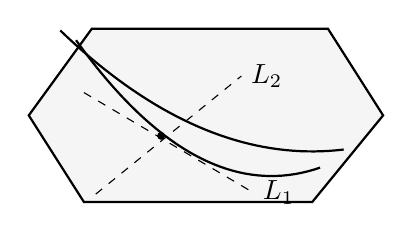
\begin{tikzpicture}[scale=1.0]
		% 曲面示意 (用椭圆表示)
		\draw[thick, fill=gray!8] (-2.1,0) -- (-1.3,1.1) -- (1.7,1.1) -- (2.4,0) -- (1.5,-1.1) -- (-1.4,-1.1) -- cycle;
		% 两条横截曲线
		\draw[thick] plot[domain=-1.7:1.9, samples=40] (\x, {0.15*\x*\x - 0.45*\x - 0.12});
		\draw[thick] plot[domain=-1.5:1.6, samples=40] (\x, {-0.5 - 0.55*\x + 0.28*\x*\x});
		% 交点与切线
		\fill (-0.42,-0.26) circle (0.05);
		\draw[dashed] (-1.4,0.29) -- (0.75,-0.98) node[right] {$L_1$};
		\draw[dashed] (-1.25,-1.0) -- (0.6,0.5) node[right] {$L_2$};
	\end{tikzpicture}
	\caption{曲面上横截的曲线}
	\label{fig:2.1}
\end{figure}

对子空间 $\Theta_{Y_i,x} \subset \Theta_{X,x}$ 用不等式 \eqref{eq:1.49} 与不等式 $\operatorname{codim} \Theta_{Y_i,x} \le \operatorname{codim}_X Y_i$, 可见 \eqref{eq:2.17} 蕴含等式
\[
	\dim \Theta_{Y_i,x} = \dim Y_i,
\]
即每个 $Y_i$ 在 $x$ 处非奇异; 还蕴含等式
\[
	\operatorname{codim}_{\Theta_{X,x}} \Bigl( \bigcap_{i=1}^{r} \Theta_{Y_i,x} \Bigr) = \sum_{i=1}^{r} \operatorname{codim} \Theta_{Y_i,x},
\]
即向量子空间 $\Theta_{Y_i,x} \subset \Theta_{X,x}$（在给定维数下交尽可能小这一意义上）横截. 由包含关系 $\bigcap_{i=1}^r \Theta_{Y_i,x} \supset \Theta_{Y,x}$（其中 $Y = \bigcap Y_i$）, 同样可推出 $Y$ 在 $x$ 处非奇异.

于是定理~\ref{thm:local-params-transversal} 断言子簇 $V(u_i)$ 横截.

设 $X'$ 是 $x$ 的使 $\bigcap X'_i = x = (0, \ldots, 0)$ 的仿射邻域. 若 $X' \subset \A^N$ 而 $t_i$ 是 $\A^N$ 的坐标, 则 $x$ 由 $t_1 = \cdots = t_N = 0$ 定义, 而 $\bigcap X'_i$ 在 $X'$ 中由 $u_1 = \cdots = u_n = 0$ 定义. 由 Nullstellensatz 得, 对某个 $k > 0$ 有 $(t_1, \ldots, t_N)^k \subset (u_1, \ldots, u_n)$, 这里 $(t_1, \ldots, t_N)$ 与 $(u_1, \ldots, u_n)$ 表示 $k[X']$ 中的理想. 对 $\mathcal O_x$ 中的理想 $(t_1, \ldots, t_N)$ 与 $(u_1, \ldots, u_n)$ 更是如此. 注意 $(t_1, \ldots, t_N) = \mathfrak m_x$, 故 $\mathfrak m_x^k \subset (u_1, \ldots, u_n)$. 事实上更强的结论成立.

\begin{theorem}\label{thm:params-generate}
	$x$ 处的局部参数生成 $\mathcal O_x$ 的极大理想 $\mathfrak m_x$.
\end{theorem}

\begin{proof}
	这是 Nakayama 引理（原书附录命题 A.11）作用于作为 $\mathcal O_x$-模的极大理想 $\mathfrak m_x$ 的直接推论. 由 §1.1 的引理, $\mathfrak m_x$ 是有限 $\mathcal O_x$-模. 既然局部参数生成 $\mathfrak m_x/\mathfrak m_x^2$, 由 Nakayama 引理它们生成 $\mathfrak m_x$. 定理证毕.
\end{proof}

\begin{example}[自由作用的商]\label{exam:quotient-nonsingular}
	设 $X$ 是非奇异仿射簇, $G$ 是 $X$ 的自同构的有限群, 如例~\ref{exam:quotient}. 设 $G$ 自由作用于 $X$, 即由 $g(x) = x$（$g \in G$, $x \in X$）可推出 $g = e$（$e$ 为恒等映射）. 我们证明在这些假设下商簇 $X/G$ 仍是非奇异的.

	设 $f: X \to Y = X/G$ 是例~\ref{exam:quotient} 构造的商映射, $n = \dim X = \dim Y$. 取 $x \in X$, 令 $y = f(x) \in Y$, 取 $x$ 处的局部参数 $u_1, \ldots, u_n$ 且 $u_i \in k[X]$, 则 $u_1, \ldots, u_n$ 生成 $\mathfrak m_x$. 对每个 $u_i$, 构造函数 $\bar u_i \in k[X]$, 使 $\bar u_i \equiv u_i \bmod \mathfrak m_x^2$, 且对一切 $g \ne e$ 有 $\bar u_i \in \mathfrak m_{g(x)}^2$. 为此只需把 $u_i$ 乘以一个元素 $h \in k[X]$ 的平方, 其中 $h(x) = 1$ 而对一切 $g \ne e$ 有 $h(g(x)) = 0$.

	令 $v_i = S(\bar u_i)$, 其中平均算子 $S$ 如原书附录命题 A.6 与例~\ref{exam:quotient}. 既然 $g \ne e$ 时 $g^* \bar u_i \in \mathfrak m_x^2$, 有 $v_i \equiv \frac{1}{|G|} u_i \bmod \mathfrak m_x^2$, 故 $v_1, \ldots, v_n$ 是 $x$ 处的局部参数. 但 $v_i \in k[Y]$ 且 $v_i(y) = 0$. 我们证明 $\mathfrak m_y = (v_1, \ldots, v_n)$. 设 $h \in \mathfrak m_y \cap k[Y]$, 则 $f^*(h) \in \mathfrak m_x$ 且 $f^*(h) = \sum h_i v_i$. 对此应用算子 $S$, 由 $S(f^*(h)) = f^*(h)$ 与 $S(v_i) = v_i$ 得 $f^*(h) = \sum S(h_i)\, v_i$. 于是 $\dim \mathfrak m_y/\mathfrak m_y^2 \le n$, 从而 $y$ 非奇异.
\end{example}

值得指出, 点 $x$ 的非奇异性由局部环 $\mathcal O_x$ 的纯代数性质刻画. 按定义, $x \in X$ 非奇异当且仅当 $\dim_k \mathfrak m_x/\mathfrak m_x^2 = \dim_x X$. 等式左端对任何 Noether 局部环 $\mathcal O$ 都有定义; 右端也可表述为局部环 $\mathcal O_x$ 的性质. 事实上, 由定理~\ref{thm:all-components} 与推论~\ref{cor:subvariety-dims}, $X$ 在 $x$ 处的维数可定义为使存在 $r$ 个函数 $u_1, \ldots, u_r \in \mathfrak m_x$ 且在 $x$ 的某邻域中由 $u_1 = \cdots = u_r = 0$ 定义的集合恰为 $x$ 的最小 $r$. 由 Nullstellensatz, 这一性质等价于对某个 $k > 0$ 有 $(u_1, \ldots, u_r) \supset \mathfrak m_x^k$.

对极大理想为 $\mathfrak m$ 的任意 Noether 局部环 $\mathcal O$, 使存在 $r$ 个函数 $u_1, \ldots, u_r \in \mathfrak m$ 且对某个 $k > 0$ 有 $(u_1, \ldots, u_r) \supset \mathfrak m^k$ 的最小数 $r$ 称为 $\mathcal O$ 的维数, 记作 $\dim \mathcal O$. 由 Nakayama 引理, 理想 $\mathfrak m$ 本身可由 $n$ 个元素生成, 其中 $n = \dim_{\mathcal O/\mathfrak m}(\mathfrak m/\mathfrak m^2)$, 故
\[
	\dim \mathcal O \le \dim_{\mathcal O/\mathfrak m} (\mathfrak m/\mathfrak m^2).
\]
若 $\dim \mathcal O = \dim_{\mathcal O/\mathfrak m}(\mathfrak m/\mathfrak m^2)$, 就称局部环 $\mathcal O$ 为\emph{正则}的. 于是 $x$ 是非奇异点当且仅当局部环 $\mathcal O_x$ 正则. 这就是点的非奇异性的代数含义.

\subsection{幂级数展开}

把幂级数与局部环 $\mathcal O_x$ 的元素联系起来的想法基于如下论证. 对任何函数 $f \in \mathcal O_x$, 令 $f(x) = \alpha_0$, $f_1 = f - \alpha_0$; 则 $f_1 \in \mathfrak m_x$. 设 $u_1, \ldots, u_n$ 是 $x$ 处的一组局部参数. 按定义, $u_1, \ldots, u_n$ 生成整个向量空间 $\mathfrak m_x/\mathfrak m_x^2$, 故存在 $\alpha_1, \ldots, \alpha_n \in k$ 使 $f_1 - \sum_{i=1}^n \alpha_i u_i \in \mathfrak m_x^2$. 令 $f_2 = f_1 - \sum \alpha_i u_i = f - \alpha_0 - \sum \alpha_i u_i$. 既然 $f_2 \in \mathfrak m_x^2$, 可写 $f_2 = \sum g_j h_j$, 诸 $g_j, h_j \in \mathfrak m_x$. 同上, 存在 $\beta_{ji}, \gamma_{ji} \in k$ 使
\[
	g_j - \sum_{i=1}^{n} \beta_{ji} u_i \in \mathfrak m_x^2, \qquad h_j - \sum_{i=1}^{n} \gamma_{ji} u_i \in \mathfrak m_x^2.
\]
令 $\sum_j \bigl( \sum_i \beta_{ji} u_i \bigr)\bigl( \sum_i \gamma_{ji} u_i \bigr) = \sum_{l,k=1}^{n} \alpha_{lk}\, u_l u_k$, 则 $f_2 - \sum \alpha_{lk} u_l u_k \in \mathfrak m_x^3$, 因此 $f_3 = f - \alpha_0 - \sum \alpha_i u_i - \sum \alpha_{lk} u_l u_k \in \mathfrak m_x^3$. 如此继续, 显然可找到型 $F_i \in k[T_1, \ldots, T_n]$（$\deg F_i = i$）使
\[
	f - \sum_{i=0}^{k} F_i(u_1, \ldots, u_n) \in \mathfrak m_x^{k+1}.
\]

\begin{definition}[形式幂级数环]\label{def:power-series-ring}
	变量 $(T_1, \ldots, T_n) = T$ 的\emph{形式幂级数环}是这样的环: 其元素为形如
	\begin{equation}
		\label{eq:2.18}
		\Phi = F_0 + F_1 + F_2 + \cdots
	\end{equation}
	的无穷表达式, 其中 $F_i \in k[T]$ 是 $i$ 次型; 环运算按下述规则定义: 若 $\Psi = G_0 + G_1 + G_2 + \cdots$, 则
	\[
		\Phi + \Psi = (F_0 + G_0) + (F_1 + G_1) + (F_2 + G_2) + \cdots,
	\]
	而 $\Phi\Psi = H_0 + H_1 + H_2 + \cdots$, 其中 $H_i = \sum_{j+l=i} G_j F_l$.
\end{definition}

形式幂级数环记作 $k[[T]]$. 它包含 $k$, 即 $i > 0$ 时 $F_i = 0$ 的幂级数. 若 $i$ 是使 $F_i \ne 0$ 的第一个下标, 则称 $F_i$ 为 \eqref{eq:2.18} 的首项. 乘积的首项等于首项之积, 故 $k[[T]]$ 没有零因子.

上面讨论的论证使我们可以给每个函数 $f \in \mathcal O_x$ 联系一个幂级数 $\Phi = F_0 + F_1 + F_2 + \cdots$. 于是得到如下定义.

\begin{definition}[Taylor 级数]\label{def:taylor-series}
	形式幂级数 $\Phi$ 称为函数 $f \in \mathcal O_x$ 的\emph{Taylor 级数}, 如果对每个 $k \ge 0$ 有
	\begin{equation}
		\label{eq:2.19}
		f - S_k(u_1, \ldots, u_n) \in \mathfrak m_x^{k+1}, \qquad S_k = \sum_{i=0}^{k} F_i.
	\end{equation}
\end{definition}

\begin{example}\label{exam:taylor-A1}
	设 $X = \A^1$, 坐标为 $t$, $x$ 是点 $t = 0$. 于是 $\mathfrak m_x = (t)$, 且可以给任何有理函数 $f(t) = P(t)/Q(t)$（$Q(0) \ne 0$）联系幂级数 $\sum_{m=0}^{\infty} \alpha_m t^m$, 使
	\[
		\frac{P(t)}{Q(t)} - \sum_{m=0}^{k} \alpha_m t^m \equiv 0 \bmod t^{k+1},
		\qquad\text{即}\qquad
		P(t) - Q(t) \sum_{m=0}^{k} \alpha_m t^m \equiv 0 \bmod t^{k+1}.
	\]
	这就是用待定系数法求有理函数幂级数系数的通常程序. 例如
	\[
		\frac{1}{1-t} = \sum_{m=0}^{\infty} t^m, \quad\text{因为}\quad \frac{1}{1-t} - \sum_{m=0}^{k} t^m = \frac{t^{k+1}}{1-t} \equiv 0 \bmod t^{k+1}.
	\]
	对应 $f \mapsto \Phi$ 实质上依赖于局部参数组 $u_1, \ldots, u_n$ 的选取.
\end{example}

刚才给出的论证证明了下面的断言.

\begin{theorem}\label{thm:taylor-exists}
	每个函数至少有一个 Taylor 级数.
\end{theorem}

到目前为止我们实质上没有用到 $x$ 非奇异, 只用到 $u_1, \ldots, u_n$ 生成 $\mathfrak m_x/\mathfrak m_x^2$. 现在使用 $x$ 的非奇异性.

\begin{theorem}\label{thm:taylor-unique}
	若 $x$ 非奇异, 则函数的 Taylor 级数唯一.
\end{theorem}

\begin{proof}
	显然只需证明函数 $f = 0$ 的任何 Taylor 级数都等于 $0$. 由 \eqref{eq:2.19}, 这等价于断言: 若 $u_1, \ldots, u_n$ 是非奇异点 $x$ 的局部参数, 则对 $k$ 次型 $F_k(T_1, \ldots, T_n)$,
	\begin{equation}
		\label{eq:2.20}
		F_k(u_1, \ldots, u_n) \in \mathfrak m_x^{k+1} \implies F_k(T_1, \ldots, T_n) = 0.
	\end{equation}
	设不然. 经非退化线性变换, 可使 $F_k$ 中 $T_n^k$ 的系数非零. 事实上, 该系数等于 $F_k(0, \ldots, 0, 1)$, 而若 $F_k(\alpha_1, \ldots, \alpha_n) \ne 0$（既然 $F_k \ne 0$, 这样的 $\alpha_1, \ldots, \alpha_n$ 当然存在）, 只需施行把向量 $(\alpha_1, \ldots, \alpha_n)$ 变到 $(0, \ldots, 0, 1)$ 的线性变换. 于是可设
	\[
		F_k(T_1, \ldots, T_n) = \alpha\, T_n^k + G_1(T_1, \ldots, T_{n-1})\, T_n^{k-1} + \cdots + G_k(T_1, \ldots, T_{n-1}),
	\]
	其中 $\alpha \ne 0$, 诸 $G_i$ 是 $T_1, \ldots, T_{n-1}$ 的 $i$ 次型.

	由定理~\ref{thm:params-generate} 容易推出, $\mathfrak m_x^{k+1}$ 的任何元素都可写成系数在 $\mathfrak m_x$ 中的 $u_1, \ldots, u_n$ 的 $k$ 次型. 于是 \eqref{eq:2.20} 左端可表为
	\begin{equation}
		\label{eq:2.21}
		\begin{split}
			\alpha\, u_n^k + G_1&(u_1, \ldots, u_{n-1})\, u_n^{k-1} + \cdots + G_k(u_1, \ldots, u_{n-1}) \\
			={}& \mu\, u_n^k + H_1(u_1, \ldots, u_{n-1})\, u_n^{k-1} + \cdots + H_k(u_1, \ldots, u_{n-1}),
		\end{split}
	\end{equation}
	其中 $\mu \in \mathfrak m_x$, 诸 $H_i$ 是 $i$ 次型. 由此得 $(\alpha - \mu)\, u_n^k \in (u_1, \ldots, u_{n-1})$. 既然 $\alpha \ne 0$, 有 $\alpha - \mu \notin \mathfrak m_x$ 而 $(\alpha - \mu)^{-1} \in \mathcal O_x$, 故 $u_n^k \in (u_1, \ldots, u_{n-1})$.

	于是 $V(u_n) \supset V(u_1) \cap \cdots \cap V(u_{n-1})$, 从而 $\Theta_n \supset \Theta_1 \cap \cdots \cap \Theta_{n-1}$（$\Theta_i$ 是 $V(u_i)$ 在 $x$ 处的切空间）, 故 $\Theta_1 \cap \cdots \cap \Theta_n = \Theta_1 \cap \cdots \cap \Theta_{n-1}$, 于是 $\dim \Theta_1 \cap \cdots \cap \Theta_n \ge 1$, 与定理~\ref{thm:local-params-transversal} 矛盾. 定理证毕.
\end{proof}

于是我们得到一个唯一确定的映射 $\tau: \mathcal O_x \to k[[T]]$, 把每个函数送到它的 Taylor 级数. 基于 $\tau$ 的定义 \eqref{eq:2.19} 的简单验证表明它是同态, 验证留给读者.

$\tau$ 的核是什么? 若对函数 $f \in \mathcal O_x$ 有 $\tau(f) = 0$, 则由 \eqref{eq:2.19} 这意味着对一切 $k$ 有 $f \in \mathfrak m_x^{k+1}$, 换言之 $f \in \bigcap_{k=0}^{\infty} \mathfrak m_x^k$. 于是我们讨论的是分析中在某点各阶导数全为 $0$ 的函数的类似物. 在我们的情形这样的函数必为 $0$, 这由原书附录命题 A.12 与 §1.1 的引理得出.

作为推论我们得到下面的结果.

\begin{theorem}\label{thm:taylor-injective}
	函数 $f \in \mathcal O_x$ 由它的任何 Taylor 级数唯一确定. 换言之, $\tau$ 是局部环 $\mathcal O_x$ 到形式幂级数环 $k[[T]]$ 的同构嵌入.
\end{theorem}

注意, 本节至今没有用到簇 $X$ 的不可约性. 反过来, 定理~\ref{thm:taylor-injective} 使我们可以对不可约性作出某些推断.

\begin{theorem}\label{thm:unique-component}
	若 $x$ 是 $X$ 的非奇异点, 则经过 $x$ 的 $X$ 的分支只有一个.
\end{theorem}

\begin{proof}
	把 $X$ 换成含于 $X' = X \setminus \bigcup Z_i$ 的 $x$ 的仿射邻域 $U$, 其中诸 $Z_i$ 是 $X$ 的不经过 $x$ 的分支. 那么 $k[U] \subset \mathcal O_x$. 由定理~\ref{thm:taylor-injective}, $\mathcal O_x$ 同构于形式幂级数环 $k[[T]]$ 的子环. 既然 $k[[T]]$ 没有零因子, 同构于其子环的 $k[U]$ 也没有. 故 $U$ 不可约, 即定理所断言. 定理证毕.
\end{proof}

\begin{corollary}\label{cor:singular-closed}
	代数簇 $X$ 的奇异点集是闭集.
\end{corollary}

\begin{proof}
	设 $X = \bigcup X_i$ 是不可约分解. 由定理~\ref{thm:unique-component}, $X$ 的奇异点集是诸 $X_i \cap X_j$（$i \ne j$）与诸 $X_i$ 的奇异点集之并; 作为有限多个闭集之并, 它是闭集. 推论证毕.
\end{proof}

若 $x$ 是奇异点, 我们至多只能把元素 $f \in \mathcal O_x$ 送到剩余类序列 $\xi_n = f + \mathfrak m_x^n \in \mathcal O_x/\mathfrak m_x^n$. 该序列有如下相容性: 若 $\theta_{n+1}: \mathcal O_x/\mathfrak m_x^{n+1} \to \mathcal O_x/\mathfrak m_x^n$ 是商映射, 则 $\theta_{n+1}(\xi_{n+1}) = \xi_n$. 全部这样的相容序列 $\{\xi_n\}$ 按分量加法与乘法组成一个环 $\widehat{\mathcal O}_x$, 称为 $\mathcal O_x$ 的\emph{完备化}.

我们刚定义了同态 $\tau: \mathcal O_x \to \widehat{\mathcal O}_x$, $\tau(f) = \{\xi_n\}$, $\xi_n = f + \mathfrak m_x^n$. 与非奇异点情形同样的论证表明 $\tau$ 是单射. 环 $\widehat{\mathcal O}_x$ 是局部的, 其极大理想 $\mathfrak M$ 由满足 $\xi_n \in \mathfrak m_x$ 的相容序列 $\{\xi_n\}$ 组成. 可以证明, 对 $\widehat{\mathcal O}_x$ 再施行同一构造不会得到新东西, 即 $(\widehat{\mathcal O}_x)\widehat{} = \widehat{\mathcal O}_x$, 且此时 $\tau$ 是同构.

若 $x$ 非奇异, 则 $\widehat{\mathcal O}_x$ 就是形式幂级数环. 一般地, $\widehat{\mathcal O}_x$ 是奇异点的重要特征: 若对 $x \in X$ 与 $y \in Y$ 完备局部环 $\widehat{\mathcal O}_x$ 与 $\widehat{\mathcal O}_y$ 同构, 就称簇 $X$ 与 $Y$ 在这些点的邻域中形式解析等价. 既然 $n$ 维簇的非奇异点 $x$ 的局部环 $\widehat{\mathcal O}_x$ 同构于 $\A^n$ 的点 $x'$ 的局部环的完备化, 同维数一切簇的一切非奇异点都有形式解析等价的邻域. 比较 §3 习题 8--16.

\subsection{实域与复域上的簇}

设 $k = \R$ 或 $\CC$. 我们证明此时函数 $f \in \mathcal O_x$ 的形式 Taylor 级数对小的 $T_1, \ldots, T_n$ 收敛.

设 $X \subset \A^N$ 是簇, $\mathfrak A_X = (F_1, \ldots, F_m)$, $\dim_x X = n$. 若 $x \in X$ 是非奇异点, 则矩阵 $\bigl( \partial F_i/\partial T_j(x) \bigr)$ 的秩为 $N - n$. 设
\begin{equation}
	\label{eq:2.22}
	\det \Bigl| \frac{\partial F_i}{\partial T_j}(x) \Bigr|_{\substack{i = 1, \ldots, N-n \\ j = n+1, \ldots, N}} \ne 0,
\end{equation}
且 $x$ 是原点. 那么前 $n$ 个坐标在 $X$ 上的限制 $t_1, \ldots, t_n$ 构成 $X$ 在 $x$ 处的局部参数组. 用 $X'$ 表示由
\begin{equation}
	\label{eq:2.23}
	F_1 = \cdots = F_{N-n} = 0
\end{equation}
定义的簇的经过 $x$ 的全部分支之并. 由 \eqref{eq:2.22}, $X'$ 在 $x$ 处的切空间 $\Theta'$ 的维数等于 $n$; 由相交维数定理, $\dim_x X' \ge n$. 既然 $\dim \Theta' \ge \dim_x X'$, 得 $\dim_x X' = n$ 且 $x$ 是 $X'$ 的非奇异点. 由此并由定理~\ref{thm:unique-component} 得 $X'$ 不可约. 显然 $X' \supset X$, 故 $\dim X' = \dim X$ 蕴含 $X' = X$.

于是 $X$ 可在 $x$ 的某邻域中由满足 \eqref{eq:2.22} 的 $N - n$ 个方程 \eqref{eq:2.23} 定义. 由隐函数定理（例如见 Goursat \cite[第 IX 章 \S\S 187--190]{goursat1916} 或 Fleming \cite[\S 4.6]{fleming1977}）, 存在 $n$ 个变量 $T_1, \ldots, T_n$ 的幂级数组 $\Phi_1, \ldots, \Phi_{N-n}$ 与 $\varepsilon > 0$, 使 $\Phi_j(T_1, \ldots, T_n)$ 对一切 $|T_i| < \varepsilon$ 收敛, 且
\begin{equation}
	\label{eq:2.24}
	F_i\bigl( T_1, \ldots, T_n, \Phi_1(T), \ldots, \Phi_{N-n}(T) \bigr) = 0;
\end{equation}
而且幂级数 $\Phi_1, \ldots, \Phi_{N-n}$ 的系数由关系 \eqref{eq:2.24} 唯一确定.

另一方面, 设取 $t_1, \ldots, t_n$ 为局部参数, 则形式幂级数 $\tau(T_{n+1}), \ldots, \tau(T_N)$ 也满足 \eqref{eq:2.24}, 故必与 $\Phi_1, \ldots, \Phi_{N-n}$ 一致, 于是当 $|T_j| < \varepsilon$（$j = 1, \ldots, n$）时 $\tau(T_{n+1}), \ldots, \tau(T_N)$ 收敛.

任何函数 $f \in \mathcal O_x$ 可写成 $f = P/Q$ 的形式, 其中 $P = P(T_1, \ldots, T_n)$ 与 $Q = Q(T_1, \ldots, T_n)$ 是多项式且 $Q(x) \ne 0$; 于是
\[
	\tau(f) = \frac{P(\tau(T_1), \ldots, \tau(T_n))}{Q(\tau(T_1), \ldots, \tau(T_n))}.
\]
$\tau(f)$ 的收敛性由幂级数收敛性的标准定理得出.

同样可证: 若 $u_1, \ldots, u_n$ 是另一组局部参数, 则行列式 $\det \bigl| \partial \tau(u_i)/\partial T_j(0, \ldots, 0) \bigr|$ 非零, 而 $t_1, \ldots, t_n$ 关于局部参数组 $u_1, \ldots, u_n$ 的 Taylor 级数由反解级数 $\tau(u_i) = \Phi_i(T_1, \ldots, T_n)$（$i = 1, \ldots, n$）得到, 故也有正收敛半径. 因此对 $f \in \mathcal O_x$, 无论取哪组局部参数, 级数 $\tau(f)$ 都有正收敛半径.

隐函数定理不仅断言收敛级数 $\Phi_1, \ldots, \Phi_{N-n}$ 存在, 而且断言存在 $\eta > 0$, 使满足 $|t_i| < \eta$（$i = 1, \ldots, N$）的任何点 $(t_1, \ldots, t_N) \in X$ 都形如 $t_{n+i} = \Phi_i(t_1, \ldots, t_n)$（$i = 1, \ldots, N-n$）. 由此可知 $(t_1, \ldots, t_N) \mapsto (t_1, \ldots, t_n)$ 是集合 $\{\, (t_1, \ldots, t_N) \in X \mid |t_i| < \eta \,\}$ 到 $n$ 维空间中某区域的双射同胚.

既然在我们的情形 $k = \R$ 或 $\CC$, $k$ 上的射影空间 $\PP^N$ 是拓扑空间, 代数簇 $X \subset \PP^N$ 也是拓扑空间. 分别在 $k = \R$ 或 $\CC$ 的情形, $X$ 上的这个拓扑称为 $X$ 的实拓扑或复拓扑. 这个拓扑及由它导出的概念, 不应与至今使用的具有拓扑字面的术语（闭集, 邻域, 开集, 闭包等）相混淆.

前面的论证表明: 对 $n$ 维簇 $X$, 任何非奇异点在实拓扑中有一个同胚于 $\R^n$ 中某区域的邻域. 故若 $X$ 的每点都非奇异, 则 $X$ 是拓扑意义上的 $n$ 维流形. 若 $k = \CC$, 非奇异点 $x \in X$ 在复拓扑中有同胚于 $n$ 维复空间 $\CC^n$ 中某区域的邻域, 从而同胚于 $\R^{2n}$ 中某区域. 因此若 $X$ 的一切点都非奇异, 则 $X$ 是 $2n$ 维流形.

容易证明, $k = \R$ 或 $\CC$ 时 $\PP^N$ 在实拓扑或复拓扑中是紧的, 于是射影簇 $X$ 是紧的. 若 $k = \CC$, 反之亦然: 复拓扑中紧的拟投影簇是射影簇（见原书第 7 章第 2.6 节习题 2）.

最后指出, 本节所述一切（上一段除外）都可逐字逐句地搬到 $k$ 是 $p$ 进数域的情形.

\subsection{第 2 节习题}

\begin{compactenum}
	\item 证明: 对 $n$ 维簇 $X$, 使给定的 $n$ 个函数不构成局部参数组的点集是闭集.
	\item 证明: 多项式 $f \in k[T] = k[\A^1]$ 在点 $T = \alpha$ 处是局部参数, 当且仅当 $\alpha$ 是 $f$ 的单根.
	\item 证明: 形式幂级数 $\Phi = F_0 + F_1 + \cdots$ 在 $k[[T]]$ 中可逆, 当且仅当 $F_0 \ne 0$.
	\item 设 $T$ 是未定元. 考虑形如 $\alpha_{-n} T^{-n} + \alpha_{-n+1} T^{-n+1} + \cdots + \alpha_0 + \alpha_1 T + \cdots$ 的表达式组成的环 $k((T))$. 证明 $k((T))$ 是域, 且同构于 $k[[T]]$ 的分式域.（它称为形式 Laurent 级数域.）
	\item 设 $S \subset \A^2$ 是由 $X^2 + Y^2 = 1$ 给出的圆, 基域 $k$ 特征为 $0$. 证明 $X$ 在 $x = (0,1)$ 处是局部参数, 且 $Y$ 的 Taylor 展开为
	\[
		\tau(Y) = \sum_{n=0}^{\infty} \frac{(-1)^n\, (1/2)(1/2 - 1) \cdots (1/2 - n + 1)}{n!}\, X^{2n}.
	\]
	\item 证明: 若 $x$ 是奇异点, 则任何函数 $f \in \mathcal O_x$ 都有无穷多个不同的 Taylor 级数.
	\item 设 $X = \A^1$ 而 $x \in X$. 证明 $\tau(\mathcal O_x)$ 不是整个 $k[[T]]$.
\end{compactenum}

\section{非奇异点的性质}

\subsection{余维 \texorpdfstring{$1$}{1} 子簇}

局部环理论使我们能够证明非奇异簇的一个重要性质, 它是定理~\ref{thm:codim1-principal} 的类似物. 所讨论的问题是: 余维 $1$ 子簇 $Y \subset X$ 能否由单个方程定义. 对奇异簇, 这一性质一般不成立（比较推论~\ref{cor:thm121-fails}）; 但我们证明它在非奇异簇上局部成立. 为陈述结果, 引入如下定义.

\begin{definition}[局部方程]\label{def:local-equations}
	函数 $f_1, \ldots, f_m \in \mathcal O_x$ 称为子簇 $Y \subset X$ 在 $x$ 的某邻域中的\emph{局部方程}, 如果存在 $x$ 的仿射邻域 $X'$ 使 $f_1, \ldots, f_m \in k[X']$ 且在 $k[X']$ 中有 $\mathfrak a_{Y'} = (f_1, \ldots, f_m)$, 其中 $Y' = Y \cap X'$.
\end{definition}

用 $x$ 的局部环 $\mathcal O_x$ 的语言重述这一条件是方便的. 考虑由在 $x$ 的某邻域中在 $Y$ 上为零的函数 $f \in \mathcal O_x$ 组成的理想 $\mathfrak a_{Y,x} \subset \mathcal O_x$. 对仿射簇 $X$, 显然
\[
	\mathfrak a_{Y,x} = \{\, f = u/v \mid u, v \in k[X],\ u \in \mathfrak a_Y,\ v(x) \ne 0 \,\},
\]
而若 $Y$ 的全部分支都经过 $x$, 则 $\mathfrak a_Y = \mathfrak a_{Y,x} \cap k[X]$.

\begin{lemma}\label{lem:local-equations-ideal}
	函数 $f_1, \ldots, f_m \in \mathcal O_x$ 是 $Y$ 在 $x$ 的某邻域中的局部方程, 当且仅当 $\mathfrak a_{Y,x} = (f_1, \ldots, f_m)$.
\end{lemma}

\begin{proof}
	若在 $k[X]$ 中 $\mathfrak a_Y = (f_1, \ldots, f_m)$, 那么显然在 $\mathcal O_x$ 中也有 $\mathfrak a_{Y,x} = (f_1, \ldots, f_m)$. 反之, 设 $\mathfrak a_{Y,x} = (f_1, \ldots, f_m)$（诸 $f_i \in \mathcal O_x$）, 并设 $\mathfrak a_Y = (g_1, \ldots, g_s)$（诸 $g_i \in k[X]$）. 既然 $g_i \in \mathfrak a_{Y,x}$, 可写
	\begin{equation}
		\label{eq:2.25}
		g_i = \sum_{j=1}^{m} h_{ij} f_j, \qquad h_{ij} \in \mathcal O_x.
	\end{equation}
	函数 $f_i$ 与 $h_{ij}$ 都在 $x$ 的某个主开邻域 $U$ 中正则. 设 $U = X \setminus V(g)$（$g \in k[X]$）, 则 $k[U]$ 由形如 $u/g^l$（$u \in k[X]$, $l \ge 0$）的元素组成. 于是由 \eqref{eq:2.25}, 在 $k[U]$ 中有
	\[
		(g_1, \ldots, g_s) = \mathfrak a_Y\, k[U] \subset (f_1, \ldots, f_m).
	\]
	我们证明 $\mathfrak a_Y\, k[U] = \mathfrak a_{Y'}$（此时 $Y' = Y \cap U$）. 由此得 $\mathfrak a_{Y'} \subset (f_1, \ldots, f_m)$; 又 $f_i \in \mathfrak a_{Y'}$, 便得引理的断言.

	剩下证明 $\mathfrak a_Y\, k[U] = \mathfrak a_{Y'}$. 包含关系 $\mathfrak a_Y\, k[U] \subset \mathfrak a_{Y'}$ 是显然的. 设 $v \in \mathfrak a_{Y'}$, 则 $v = u/g^l$（$u \in k[X]$）, 于是 $u = v g^l$, 故 $u \in \mathfrak a_Y$; 又 $1/g^l \in k[U]$, 得 $v = u/g^l \in \mathfrak a_Y\, k[U]$. 引理证毕.
\end{proof}

我们的目标是证明下面的结果.

\begin{theorem}\label{thm:codim1-local-eq}
	余维 $1$ 的不可约子簇 $Y \subset X$ 在任何非奇异点 $x \in X$ 的某邻域中有局部方程.
\end{theorem}

证明完全循定理~\ref{thm:codim1-principal} 的步骤. 不过那里用到了 $k[T]$ 是唯一分解整环这一事实; 这里起 $k[T]$ 作用的是局部环 $\mathcal O_x$, 它具有类似的性质.

\begin{theorem}\label{thm:local-ufd}
	非奇异点的局部环 $\mathcal O_x$ 是唯一分解整环.
\end{theorem}

定理~\ref{thm:local-ufd} 的证明基于先建立幂级数环 $k[[T]]$ 是唯一分解整环. 这是一个相当初等的事实, 与多项式环的相应结果类似; 我们只指出证明的主要步骤. 完全初等的（不依赖本书其余部分的）证明见 Zariski--Samuel \cite[第 VII 章第 1 节定理 6]{zariski-samuel1960}.

称幂级数 $\Phi(T_1, \ldots, T_n)$ 关于变量 $T_n$ 是正则的, 如果它的首项型（设为 $m$ 次）含有项 $c_m T_n^m$（$c_m \ne 0$）. 变量 $T_1, \ldots, T_n$ 的线性变换显然诱导 $k[[T]]$ 的自同构; 特别地, 可施行线性变换使任何给定的非零幂级数 $\Phi$ 关于 $T_n$ 正则.

\begin{lemma}[Weierstrass 预备定理]\label{lem:weierstrass-prep}
	设幂级数 $\Phi \in k[[T]]$ 关于 $T_n$ 正则且首项型为 $m$ 次, 则存在常数项非零的幂级数 $U \in k[[T]]$, 使 $\Phi U$ 是系数在 $k[[T_1, \ldots, T_{n-1}]]$ 中的关于 $T_n$ 的多项式, 即
	\[
		\Phi U = T_n^m + R_1 T_n^{m-1} + \cdots + R_m, \qquad R_i = R_i(T_1, \ldots, T_{n-1}) \in k[[T_1, \ldots, T_{n-1}]].
	\]
	证明见 Zariski--Samuel \cite[第 VII 章第 1 节定理 5]{zariski-samuel1960}.
\end{lemma}

\begin{lemma}\label{lem:power-series-ufd}
	形式幂级数环 $k[[T]]$ 是唯一分解整环.
\end{lemma}

引理~\ref{lem:weierstrass-prep} 使我们可以对变量个数作归纳来证明这一断言, 把它归结为系数在 $k[[T_1, \ldots, T_{n-1}]]$ 中的 $T_n$ 的多项式的类似命题. 详细证明见 Zariski--Samuel \cite[第 VII 章第 1 节定理 6]{zariski-samuel1960}.

\begin{proof}[定理~\ref{thm:local-ufd} 的证明]
	用 $\widehat{\mathcal O}_x$ 表示形式幂级数环, 由定理~\ref{thm:taylor-injective} 可把 $\mathcal O_x$ 视为其子环 $\mathcal O_x \subset \widehat{\mathcal O}_x$. 用 $\widehat{\mathfrak m}_x$ 表示 $\widehat{\mathcal O}_x$ 中由常数项为 $0$ 的形式幂级数组成的理想, 则 $\widehat{\mathfrak m}_x^k$ 是不含次数 $< k$ 的项的形式幂级数组成的理想. 由嵌入 $\mathcal O_x \hookrightarrow \widehat{\mathcal O}_x$ 的定义（见 \eqref{eq:2.19}）得 $\widehat{\mathfrak m}_x^k \cap \mathcal O_x = \mathfrak m_x^k$. 于是原书附录命题 A.14 的条件满足, 它保证由 $\widehat{\mathcal O}_x$ 是唯一分解整环（引理~\ref{lem:power-series-ufd}）可推出 $\mathcal O_x$ 是唯一分解整环. 定理证毕.
\end{proof}

\begin{proof}[定理~\ref{thm:codim1-local-eq} 的证明]
	如前所述, 证明与定理~\ref{thm:codim1-principal} 完全相同. 既然断言是局部的, 可设 $X$ 仿射. 取任一在 $Y$ 上为零的函数 $f \in \mathcal O_x$, 把 $f$ 在 $\mathcal O_x$ 中分解为素因子之积. 由 $Y$ 的不可约性, 某个因子也在 $Y$ 上为零; 把它记作 $g$, 我们证明它是 $Y$ 的局部方程. 把 $X$ 换成更小的 $x$ 的仿射邻域, 可设 $g$ 在 $X$ 上正则.

	既然 $V(g) \supset Y$ 且二者都是余维 $1$ 子簇, 有 $V(g) = Y \cup Y'$. 若 $Y' \ni x$, 则存在函数 $h$ 与 $h'$, 使 $hh'$ 在 $V(g)$ 上为零而 $h$ 与 $h'$ 都不在 $V(g)$ 上为零. 于是对某个 $r$, 在 $k[X]$ 中 $g \mid (hh')^r$, 从而更加在 $\mathcal O_x$ 中 $g \mid (hh')^r$. 既然 $\mathcal O_x$ 是唯一分解整环, 由此得在 $\mathcal O_x$ 中 $g$ 整除 $h$ 或 $h'$. 于是 $h$ 或 $h'$ 在 $x$ 的某邻域中在 $V(g)$ 上为零, 从而（过渡到更小的邻域后）在整个 $V(g)$ 上为零, 与 $Y' \ni x$ 矛盾. 故 $Y' \not\ni x$; 再把 $X$ 换成足够小的 $x$ 的仿射邻域, 可设 $V(g) = Y$.

	现在若 $u$ 在 $Y$ 上为零, 则对某个 $s > 0$ 在 $k[X]$ 中 $g \mid u^s$, 从而更加在 $\mathcal O_x$ 中 $g \mid u^s$. 由此得在 $\mathcal O_x$ 中 $g \mid u$. 于是 $\mathfrak a_{Y,x} = (g)$, 定理证毕.
\end{proof}

定理~\ref{thm:codim1-local-eq} 有许多应用. 下面是第一个（比较第一章定理~\ref{thm:rational-map-regular}）.

\begin{theorem}\label{thm:rational-map-codim2}
	若 $X$ 是非奇异簇而 $\varphi: X \to \PP^n$ 是到射影空间的有理映射, 则 $\varphi$ 不正则的点集的余维数 $\ge 2$.
\end{theorem}

\begin{proof}
	回忆有理映射 $\varphi$ 的不正则点集（不定点轨迹）是闭集. 定理的断言是局部的, 只需在非奇异点 $x \in X$ 的邻域中证明. 可把 $\varphi$ 写成 $\varphi = (f_0 : \cdots : f_n)$（诸 $f_i \in k(X)$）, 且在不改变 $\varphi$ 的前提下通分, 使诸 $f_i \in \mathcal O_x$ 且在 $\mathcal O_x$ 中没有公因子. 此时 $\varphi$ 只在使 $f_0 = \cdots = f_n = 0$ 的点处不正则. 但没有余维 $1$ 子簇 $Y$ 能含于这些方程定义的集合中; 事实上, 由定理~\ref{thm:codim1-local-eq}, $\mathfrak a_{Y,x} = (g)$, 而诸 $f_i$ 在 $\mathcal O_x$ 中将以 $g$ 为公因子, 与假设矛盾. 定理证毕.
\end{proof}

\begin{corollary}\label{cor:curve-rational-regular}
	非奇异曲线到射影空间的任何有理映射都是正则的.
\end{corollary}

\begin{corollary}\label{cor:curves-birational-iso}
	双有理等价的非奇异射影曲线是同构的.
\end{corollary}

设 $k = \CC$ 是复数域. 由推论~\ref{cor:curves-birational-iso} 可知: 若两条曲线 $X'$ 与 $X''$ 双有理等价, 则 $X'$ 与 $X''$ 的复点集（带复拓扑）同胚. 事实上, 此时正则函数从而正则映射由收敛幂级数定义, 因而是连续的.

同样的结论对由实系数方程定义且存在定义在 $\R$ 上的双有理映射 $\varphi: X' \to X''$（即由实系数有理函数定义）的曲线的实点集成立. 这有时使我们能容易地推断两条曲线在 $\R$ 上不双有理等价. 例如, 由 $y^2 = x^3 - x$ 定义的曲线 $X$ 由两个连通分支组成（图~\ref{fig:2.2}）, 因此 $X$ 在 $\R$ 上不是有理的, 因为 $\PP^1$ 同胚于圆周, 只有一个连通分支.

用类似的思想可以证明曲线 $X$（$y^2 = x^3 - x$）在 $\CC$ 上也是非有理的. 为此需比较 $X$ 与 $\PP^1$ 的复点集（带复拓扑）并证明它们不同胚: 前者同胚于环面, 后者同胚于球面. 这是原书第 7 章第 3.3 节所证结果的特殊情形. 图~\ref{fig:2.3} 显示了 $X$ 的实点集作为其复点集的子集的样子.

\begin{figure}[htbp]
	\centering
	\begin{tikzpicture}[scale=1.1]
		\draw[->] (-1.6,0) -- (2.4,0) node[right] {$x$};
		\draw[->] (0,-2.0) -- (0,2.0) node[above] {$y$};
		% 有界分支 (卵形): x in [-1,0]
		\draw[thick] plot[domain=-1:0, samples=60] (\x, {sqrt(\x*\x*\x - \x)});
		\draw[thick] plot[domain=-1:0, samples=60] (\x, {-sqrt(\x*\x*\x - \x)});
		% 无界分支: x >= 1
		\draw[thick] plot[domain=1:2.1, samples=60] (\x, {sqrt(\x*\x*\x - \x)});
		\draw[thick] plot[domain=1:2.1, samples=60] (\x, {-sqrt(\x*\x*\x - \x)});
		\fill (-1,0) circle (0.035);
		\fill (0,0) circle (0.035);
		\fill (1,0) circle (0.035);
	\end{tikzpicture}
	\caption{$\R$ 上的 $y^2 = x^3 - x$}
	\label{fig:2.2}
\end{figure}

\begin{figure}[htbp]
	\centering
	\begin{tikzpicture}[scale=1.0]
		% 环面示意 (两圈椭圆)
		\draw[thick] (0,0) ellipse (2.2 and 0.85);
		\draw[thick] (0,0.25) ellipse (1.35 and 0.45);
		\fill[white] (0,0.25) ellipse (1.3 and 0.42);
		% 环面上的实点集: 两条闭曲线 (示意)
		\draw[thick, dashed] (-1.95,0.28) .. controls (-1.0,0.75) and (1.0,0.75) .. (1.95,0.28);
		\draw[thick, dashed] (-1.95,-0.28) .. controls (-1.0,-0.62) and (1.0,-0.62) .. (1.95,-0.28);
		\node[below] at (0,-1.15) {实点集（虚线）位于环面上};
	\end{tikzpicture}
	\caption{$\CC$ 上的 $y^2 = x^3 - x$}
	\label{fig:2.3}
\end{figure}

\subsection{非奇异子簇}

定理~\ref{thm:codim1-local-eq} 不能推广到余维数 $> 1$ 的子簇 $Y \subset X$（例如比较第一章 §6 习题 2）. 但对在 $x$ 处非奇异的子簇, 类似的结论成立. 我们证明一个略为精确的事实, 从一个辅助断言开始.

\begin{theorem}\label{thm:params-subvariety}
	设 $X$ 是仿射簇, $x \in X$ 是非奇异点, $u_1, \ldots, u_n$ 是 $X$ 上正则的函数且构成 $x$ 处的局部参数组. 那么对 $m \le n$, 由 $u_1 = \cdots = u_m = 0$ 定义的子簇 $Y$ 在 $x$ 处非奇异, 在 $x$ 的某仿射邻域中有 $\mathfrak a_Y = (u_1, \ldots, u_m)$, 且 $u_{m+1}, \ldots, u_n$ 构成 $Y$ 在 $x$ 处的局部参数组.
\end{theorem}

\begin{proof}
	对 $m$ 作归纳. 对 $m = 1$, 定理~\ref{thm:codim1-local-eq} 表明在 $x$ 的某仿射邻域中 $\mathfrak a_Y = (f)$. 设 $u_1 = f v$, 则 $d_x u_1 = v(x)\, d_x f$. 既然 $u_1$ 是局部参数组的元素, $d_x u_1 \ne 0$, 故 $v(x) \ne 0$, 于是在某个更小的开集中 $\mathfrak a_Y = (u_1)$. 又 $d_x u_1 \ne 0$ 推出 $x$ 是 $Y$ 的非奇异点.

	由 $\Theta_{X,x}$ 加上条件 $d_x u_1 = 0$ 显然得到切空间 $\Theta_{Y,x}$. 因此 $d_x u_2, \ldots, d_x u_n$ 构成 $\Theta_{Y,x}^*$ 的基, 即 $u_2, \ldots, u_n$ 是 $Y$ 在 $x$ 处的局部参数组.

	一般情形, 令 $X' \subset X$ 是由 $u_1 = 0$ 定义的子簇, 则 $Y \subset X'$ 在 $X'$ 中由方程 $u_2 = \cdots = u_m = 0$ 定义, 对 $m-1$ 用归纳即得. 定理证毕.
\end{proof}

现在证明在 $x$ 处非奇异的任何子簇 $Y \subset X$ 在 $x$ 的某邻域中可由定理~\ref{thm:params-subvariety} 所述的方式给出.

\begin{theorem}\label{thm:subvariety-local-params}
	设 $X$ 是簇, $Y \subset X$ 是子簇, $x \in Y$ 是 $X$ 与 $Y$ 的公共非奇异点. 那么可以选取 $X$ 在 $x$ 处的局部参数组 $u_1, \ldots, u_n$ 与 $x$ 的仿射邻域 $U$, 使在 $U$ 中 $\mathfrak a_Y = (u_1, \ldots, u_m)$.
\end{theorem}

在特殊情形 $X = \A^n$ 而 $k = \R$ 或 $\CC$, 类似的事实已在 §2.3 证明.

\begin{proof}
	切空间的包含 $\Theta_{Y,x} \hookrightarrow \Theta_{X,x}$ 对应对偶空间的满射 $\varphi: \mathfrak m_{X,x}/\mathfrak m_{X,x}^2 \to \mathfrak m_{Y,x}/\mathfrak m_{Y,x}^2$（由函数从 $X$ 限制到 $Y$ 定义）. 可以选取 $\mathfrak m_{X,x}/\mathfrak m_{X,x}^2$ 的基 $u_1, \ldots, u_n$, 使 $u_1, \ldots, u_m \in \mathfrak a_Y$ 而 $u_{m+1}, \ldots, u_n$ 在 $Y$ 上的限制构成 $\mathfrak m_{Y,x}/\mathfrak m_{Y,x}^2$ 的基. 取使诸 $u_i$ 都正则的 $x$ 的仿射邻域, 在其中考虑由 $u_1 = \cdots = u_m = 0$ 定义的子簇 $Y'$. 由构造 $Y' \supset Y$. 我们证明 $Y = Y'$, 于是断言由定理~\ref{thm:params-subvariety} 得出.

	由定理~\ref{thm:params-subvariety}, $Y'$ 在 $x$ 处非奇异, 由定理~\ref{thm:unique-component} 在 $x$ 的某邻域中不可约, 且 $\dim Y' = n - m$. 由构造显然 $\dim \Theta_{Y,x} = n - m$. 故 $Y = Y'$; 又由定理~\ref{thm:params-subvariety} 有 $\mathfrak a_{Y'} = (u_1, \ldots, u_m)$, 于是在 $x$ 的某邻域中也有 $\mathfrak a_Y = (u_1, \ldots, u_m)$. 定理证毕.
\end{proof}

\subsection{第 3 节习题}

\begin{compactenum}
	\item 证明: 若 $t$ 是代数曲线非奇异点处的局部参数, 则任何函数 $f \in \mathcal O_x$ 都可唯一地写成 $f = t^n u$ 的形式, 其中 $n \ge 0$, $u$ 是 $\mathcal O_x$ 的可逆元. 由此推出定理~\ref{thm:local-ufd} 对曲线的情形成.
	\item 证明定理~\ref{thm:local-params-transversal} 的逆: 若余维 $1$ 子簇 $D_1, \ldots, D_n$ 在 $x$ 处横截相交, 而 $u_1, \ldots, u_n$ 是它们在 $x$ 的某邻域中的局部方程, 则 $u_1, \ldots, u_n$ 构成 $x$ 处的局部参数组.
	\item 没有非奇异性假设时推论~\ref{cor:curves-birational-iso} 是否成立? 定理~\ref{thm:rational-map-codim2} 本身呢?
	\item 证明: 代数曲线 $X$ 的点 $x$ 非奇异, 当且仅当 $x$ 在 $X$ 上有局部方程.
	\item 设 $X \subset \A^3$ 是由 $x^2 + y^2 - z^2$ 给出的锥面. 证明母线 $L$（由 $x = 0$, $y = z$ 定义）在 $(0,0,0)$ 的任何邻域中没有局部方程.
	\item 设 $\varphi: \PP^2 \to \PP^2$ 是由 $\varphi(x_0 : x_1 : x_2) = (x_1 x_2 : x_0 x_2 : x_0 x_1)$ 定义的有理映射. 考虑点 $x = (1 : 0 : 0)$ 与在 $x$ 处非奇异的曲线 $C \subset \PP^2$. 由定理~\ref{thm:rational-map-codim2}, $\varphi$ 在 $C$ 上的限制在 $x$ 处正则, 因此把 $x$ 映到某点, 记作 $\varphi_C(x)$. 证明 $\varphi_{C_1}(x) = \varphi_{C_2}(x)$ 当且仅当 $C_1$ 与 $C_2$ 在 $x$ 处相切, 即 $\Theta_{C_1,x} = \Theta_{C_2,x}$.
	\item 证明: 若 $\varphi = f/g$ 是有理函数, $f$ 与 $g$ 在非奇异点 $x$ 处正则, 且幂级数 $\tau(f)$ 被 $\tau(g)$ 整除, 则 $\varphi$ 在 $x$ 处正则.（提示: 利用原书附录命题 A.14 的论证.）
	\item 下述断言将在后面的习题中使用. 设 $X \subset \A^n$ 是仿射簇, $x \in X$, $\mathfrak a_X = (f_1, \ldots, f_m)$. 证明
	\[
		\widehat{\mathcal O}_x = k[[T_1, \ldots, T_n]]/\bar{\mathfrak a}_X, \qquad \bar{\mathfrak a}_X = (\tau(f_1), \ldots, \tau(f_m)),
	\]
	其中 $\tau(f_i)$ 是 $f_i$ 如 §2.2 的 Taylor 级数.（提示: 利用 Atiyah--Macdonald \cite[第 10 章]{atiyah-macdonald1969} 的结果.）
	\item 证明: $\A^n$ 与自身的形式解析等价（即形式解析自同构）在 $0$ 的邻域中由无常数项且线性项构成的行列式非零的幂级数 $\Phi_1, \ldots, \Phi_n$ 给出.
	\item 证明: 过原点 $0 \in \A^2$ 的两条方程为 $F = 0$ 与 $G = 0$ 的平面曲线在 $0$ 的邻域中形式解析等价, 当且仅当存在 $\A^2$ 的由幂级数 $\Phi_1, \Phi_2$ 给出的形式解析自同构, 使 $F(\Phi_1, \Phi_2) = G U$, 其中 $U$ 是常数项非零的幂级数.
	\item 证明: 以 $0$ 为具有两条不同切线的二重点的任何非奇异代数曲线, 在 $0$ 的邻域中形式解析等价于曲线 $xy = 0$.（提示: 利用习题 10, 在理想 $(x,y)$ 的越来越高次幂模掉的意义下寻找 $\Phi_1, \Phi_2$.）
	\item 在特征 $0$ 的域上按形式解析等价对代数平面曲线的二重点分类.
	\item 设 $X$ 是 $\A^n$ 中方程为 $F = F_2(T) + F_3(T) + \cdots + F_k(T) = 0$ 的超曲面, 其中 $F_2(T)$ 是秩极大的二次型. 证明: $X$ 在 $0$ 的邻域中形式解析等价于二次锥面 $T_1^2 + \cdots + T_n^2 = 0$.
	\item 构造无穷多条非奇异射影曲线, 使其中任何两条在 $\R$ 上不同构.
	\item 设非奇异不可约 $n$ 维仿射簇 $X \subset \A^n$ 由方程 $F_1 = \cdots = F_m = 0$ 给出, 且对每点 $x = (x_1, \ldots, x_n) \in X$, 由 $\sum (\partial F_i/\partial T_j)(x)(T_j - x_j) = 0$ 定义的空间是 $n$ 维的. 证明此时 $\mathfrak a_X = (F_1, \ldots, F_m)$.
	\item 从习题 15 推出: 若把 Grassmann 簇 $\operatorname{Grass}(2, r)$ 的 Plücker 方程 $x \wedge x = 0$ 写成 $F_1 = \cdots = F_m = 0$, 则 $F_1, \ldots, F_m$ 生成 $\operatorname{Grass}(2, r)$ 的理想.（比较例~\ref{exam:grassmannian} 与例~\ref{exam:tangent-grassmann} 后的注记.）
\end{compactenum}

\section{双有理映射的结构}

\subsection{射影空间中的胀开}

前一节我们证明了非奇异射影曲线之间的双有理映射是同构（定理~\ref{thm:rational-map-codim2}, 推论~\ref{cor:curves-birational-iso}）. 这对高维簇不再成立. 例如, 球极投影建立非奇异二次曲面 $Q \subset \PP^3$ 与射影平面 $\PP^2$ 之间的双有理等价, 但它不是正则映射（见第一章 §4 习题 7, 并比较第一章的命题~\ref{prop:common-zero} 与推论~\ref{cor:r-forms}）. 本节定义并研究最简单且最典型的非同构双有理映射: 胀开.

考虑两个射影空间: 齐次坐标为 $x_0, \ldots, x_n$ 的 $\PP^n$ 与齐次坐标为 $y_1, \ldots, y_n$ 的 $\PP^{n-1}$. 对点 $x = (x_0 : \cdots : x_n) \in \PP^n$ 与 $y = (y_1 : \cdots : y_n) \in \PP^{n-1}$, 把积 $\PP^n \times \PP^{n-1}$ 中的点 $(x, y)$ 也记作 $(x_0 : \cdots : x_n;\, y_1 : \cdots : y_n)$. 考虑由方程
\begin{equation}
	\label{eq:2.26}
	x_i\, y_j = x_j\, y_i \qquad (i, j = 1, \ldots, n)
\end{equation}
定义的闭子簇 $\Pi \subset \PP^n \times \PP^{n-1}$.

\begin{definition}[胀开]\label{def:blowup}
	限制第一投影 $\PP^n \times \PP^{n-1} \to \PP^n$ 得到的映射 $\sigma: \Pi \to \PP^n$ 称为以 $\xi$ 为中心的\emph{胀开}\index{zhangkai@胀开}\footnote{这一概念在文献中还有许多名称: $\sigma$-过程, 单项变换, 膨胀, 二次变换等.}.
\end{definition}

用 $\xi$ 表示点 $\xi = (1 : 0 : \cdots : 0) \in \PP^n$. 若 $(x_0 : \cdots : x_n) \ne \xi$, 则由 \eqref{eq:2.26} 得 $(y_1 : \cdots : y_n) = (x_1 : \cdots : x_n)$, 于是由
\begin{equation}
	\label{eq:2.27}
	(x_0 : \cdots : x_n) \mapsto \bigl( (x_0 : \cdots : x_n),\ (x_1 : \cdots : x_n) \bigr)
\end{equation}
定义的映射 $\sigma^{-1}: \PP^n \setminus \xi \to \Pi$ 是 $\sigma$ 的逆. 然而当 $(x_0 : \cdots : x_n) = \xi$ 时, \eqref{eq:2.26} 对诸 $y_i$ 的任何取值都满足. 于是 $\sigma^{-1}(\xi) = \xi \times \PP^{n-1}$, 而 $\sigma$ 给出 $\PP^n \setminus \xi$ 与 $\Pi \setminus (\xi \times \PP^{n-1})$ 之间的同构. 点 $\xi$ 称为胀开 $\sigma$ 的中心.

我们来描述 $\Pi$ 在形如 $(\xi;\, y_1, \ldots, y_n)$ 的点的邻域中的结构. 某个 $y_i \ne 0$, 于是该点含于由 $x_0 \ne 0$, $y_i \ne 0$ 定义的 $\Pi$ 的开集 $U_i$; 在 $U_i$ 中甚至可设 $x_0 = 1$, $y_i = 1$. 此时 \eqref{eq:2.26} 取形式 $x_j = y_j x_i$（$j = 1, \ldots, n$, $j \ne i$）. 由此可知 $U_i$ 同构于以 $y_1, \ldots, \widehat{y_i}, x_i, \ldots, y_n$ 为坐标的仿射空间 $\A^n$.

特别地, 我们看到 $\Pi$ 非奇异, 从而由定理~\ref{thm:unique-component} 在每点的邻域中不可约. 稍后将看到 $\Pi$ 实际上不可约.

为此, 为对胀开的效果有更清晰的直观, 我们考虑 $\sigma$ 在过 $\xi$ 的某条直线 $L$ 上的情形. 设 $L$ 由 $x_j = \alpha_j x_i$（$j = 1, \ldots, n$, $j \ne i$）给出. 在 $L$ 上映射 \eqref{eq:2.27} 取形式
\[
	\sigma^{-1}(x_0 : \cdots : x_n) = (x_0 : \cdots : x_n;\, \alpha_1 : \cdots : 1 : \cdots : \alpha_n),
\]
其中第 $i$ 个位置是 $1$. 于是 $\sigma^{-1}$ 在 $L$ 上正则, 把 $L$ 映为曲线 $\sigma^{-1}(L) \subset \Pi$, 后者与 $\xi \times \PP^{n-1}$ 交于点 $(\xi;\, \alpha_1 : \cdots : 1 : \cdots : \alpha_n)$.

可以把这一结果解释如下: $\sigma^{-1}$ 在 $\xi$ 处不正则, 但限制在 $L$ 上考虑时得到正则映射 $\sigma^{-1}: L \to \Pi$. 用它可以把 $\sigma^{-1}$ 在 $L$ 上的定义扩张到点 $\xi$ 上; 在 $k = \R$ 或 $\CC$ 时, 这意味着对 $x \in L \setminus \xi$ 定义 $\sigma^{-1}(x)$, 而 $\sigma^{-1}(\xi)$ 由 $x$ 沿 $L$ 的方向趋于 $\xi$ 的极限定义. 然而结果依赖于 $L$ 的选取, 因为极限 $x \to \xi$ 依赖于 $x$ 接近 $\xi$ 的方向. 选取不同的直线 $L$ 就得到 $\xi \times \PP^{n-1}$ 的所有可能的点. 于是, 虽然 $\sigma^{-1}$ 在 $\xi$ 处不正则, 但消除由此产生的不定性时得到的不是 $\Pi$ 的任意点, 而只是 $\xi \times \PP^{n-1}$ 的点. 记住这幅图像, 我们说 $\sigma^{-1}$ 把 $\xi$ 胀开为 $\xi \times \PP^{n-1}$.

注意至此我们顺带证明了 $\Pi$ 的不可约性. 事实上
\[
	\Pi = (\xi \times \PP^{n-1}) \cup \overline{\bigl( \Pi \setminus (\xi \times \PP^{n-1}) \bigr)}.
\]
既然 $\Pi \setminus (\xi \times \PP^{n-1})$ 同构于 $\PP^n \setminus \xi$, 它不可约, 其闭包亦然. 于是只需证明 $\xi \times \PP^{n-1} \subset \overline{\Pi \setminus (\xi \times \PP^{n-1})}$. 但显然 $\sigma^{-1}(L) \subset \overline{\Pi \setminus (\xi \times \PP^{n-1})}$, 故 $\sigma^{-1}(L) \cap (\xi \times \PP^{n-1})$ 也含于该闭包; 而我们刚看到, 适当选取 $L$ 时, 左边是 $\xi \times \PP^{n-1}$ 的任意点.

对 $n = 2$, 映射 $\sigma: \Pi \to \PP^2$ 及其对直线 $L$ 的作用有直观图像: $\sigma^{-1}(L)$ 与直线 $\xi \times \PP^1$ 交于一点, 当 $L$ 绕 $\xi$ 旋转时该点随之移动. 于是 $\Pi$ 看起来像一圈螺线（图~\ref{fig:2.4}）.

\begin{figure}[htbp]
	\centering
	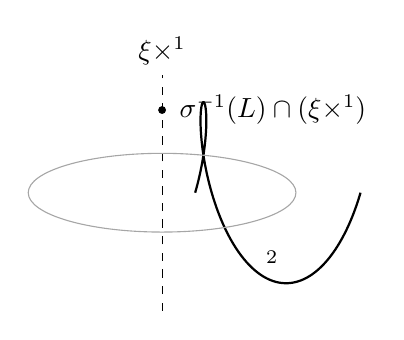
\begin{tikzpicture}[scale=1.0]
		% 螺线一圈 (示意胀开 Π → P²)
		\draw[thick, domain=0:360, samples=120, smooth, variable=\t]
			plot ({2.1*\t/360 - 1.05 + 0.42*cos(\t)}, {1.15*sin(\t)});
		% 中心轴 (ξ × P¹)
		\draw[dashed] (-1.05,-1.5) -- (-1.05,1.5) node[above] {$\xi \times \PP^1$};
		% 底部圆 (P² 的示意)
		\draw[gray!70] (-1.05,0) ellipse (1.7 and 0.5);
		\node[below] at (0.35,-0.62) {$\PP^2$};
		% 一条直线的原像与轴的交点
		\fill (-1.05,1.05) circle (0.05);
		\node[right] at (-0.95,1.05) {$\sigma^{-1}(L) \cap (\xi \times \PP^1)$};
	\end{tikzpicture}
	\caption{胀开 $\sigma: \Pi \to \PP^2$}
	\label{fig:2.4}
\end{figure}

\subsection{局部胀开}

对任意拟投影簇 $X$ 与非奇异点 $\xi \in X$, 我们现在构造一个簇 $Y$ 与映射 $\sigma: Y \to X$, 类似于 §4.1 对 $X = \PP^n$, $\xi = (1 : 0 : \cdots : 0)$ 构造的映射.

从一个辅助构造开始. 设 $X$ 是拟投影簇, $\xi \in X$ 是非奇异点, $u_1, \ldots, u_n$ 是在 $X$ 上处处正则的函数, 满足: (a) 方程 $u_1 = \cdots = u_n = 0$ 在 $X$ 中只有唯一解 $\xi$; (b) $u_1, \ldots, u_n$ 构成 $X$ 在 $\xi$ 处的局部参数组.

考虑积 $X \times \PP^{n-1}$ 及其子簇 $Y \subset X \times \PP^{n-1}$, 由满足
\[
	u_i(x)\, t_j = u_j(x)\, t_i \qquad (i, j = 1, \ldots, n)
\]
的点 $(x;\, t_1 : \cdots : t_n)$（$x \in X$, $(t_1 : \cdots : t_n) \in \PP^{n-1}$）组成. 第一投影 $X \times \PP^{n-1} \to X$ 在 $Y$ 上的限制给出的正则映射 $\sigma: Y \to X$ 称为 $X$ 的以 $\xi$ 为中心的\emph{局部胀开}.

注意这一构造一般不适用于 $X$ 是射影簇的情形, 因为它要求 $X$ 上存在非常数的处处正则函数 $u_1, \ldots, u_n$. 因此在 $X = \PP^n$ 时, 新概念并不包含前述胀开的概念. 二者的关系如下: 用 $\mathcal X \subset \PP^n$ 表示由 $x_0 \ne 0$ 定义的仿射子集, 令 $\mathcal Y = \sigma^{-1}(\mathcal X)$. 那么胀开 $\Pi \to \PP^n$ 在 $\mathcal Y$ 上诱导的映射 $\sigma: \mathcal Y \to \mathcal X$ 是一个局部胀开.

§4.1 中对 $\PP^n$ 的胀开证明的下列性质对局部胀开逐字逐句同样成立. 映射 $\sigma: Y \to X$ 正则, 且给出同构
\[
	Y \setminus (\xi \times \PP^{n-1}) \overset{\sim}{\longrightarrow} X \setminus \xi.
\]
在点 $y \in \sigma^{-1}(\xi)$ 处某个 $t_i \ne 0$, 可令 $s_j = t_j/t_i$（$j \ne i$). 此时 $Y$ 的方程取形式 $u_j = u_i s_j$（$j = 1, \ldots, n$, $j \ne i$). 由此可知 $y$ 的极大理想为
\begin{gather*}
	\mathfrak m_y = \bigl( u_1 - u_1(y), \ldots, u_n - u_n(y),\ s_1 - s_1(y), \ldots, s_n - s_n(y) \bigr) \\
	= \bigl( s_1 - s_1(y), \ldots, u_i - u_i(y), \ldots, s_n - s_n(y) \bigr),
\end{gather*}
故 $\dim \Theta_{Y,y} \le n$. 又 $\dim \overline{\sigma^{-1}(X \setminus \xi)} = n$, 故 $Y$ 在每点 $y \in \overline{\sigma^{-1}(X \setminus \xi)}$ 非奇异. 既然
\[
	Y = (\xi \times \PP^{n-1}) \cup \overline{\sigma^{-1}(X \setminus \xi)},
\]
$Y$ 或者不可约, 等于 $\sigma^{-1}(X \setminus \xi)$ 的闭包; 或者有第二个同构于 $\PP^{n-1}$ 的分支. 后一情形两个分支必相交: 否则 $\overline{\sigma^{-1}(X \setminus \xi)}$ 将在 $X \times \PP^{n-1}$ 中闭, 于是由定理~\ref{thm:projection-closed}, 其像 $X \setminus \xi \subset X$ 也闭; 而两分支的交点是奇异的, 与定理~\ref{thm:unique-component} 矛盾.

于是 $Y$ 不可约且非奇异, 且在使 $t_i \ne 0$ 的点 $y \in \sigma^{-1}(\xi)$ 处, $s_1 - s_1(y), \ldots, u_i - u_i(y), \ldots, s_n - s_n(y)$ 是局部参数.

局部胀开显然是固有映射（见定理~\ref{thm:projection-closed} 证明后的讨论）.

现在证明一个可以合理地称为``局部胀开不依赖于局部参数组 $u_1, \ldots, u_n$ 的选取''的性质.

\begin{lemma}\label{lem:blowup-independence}
	设 $v_1, \ldots, v_n$ 是 $X$ 上满足上述条件 (a) 与 (b) 的另一组函数, $\sigma': Y' \to X$ 是用 $v_1, \ldots, v_n$ 如上构造的局部胀开. 那么存在同构 $\varphi: Y \to Y'$, 使图表
	\[
		\begin{tikzcd}
			Y \ar[rr, "\varphi"] \ar[dr, swap, "\sigma"] & & Y' \ar[dl, "\sigma'"] \\
			& X &
		\end{tikzcd}
	\]
	交换.
\end{lemma}

\begin{proof}
	我们有 $Y' \subset X \times \PP^{n-1}$, 其中 $\PP^{n-1}$ 的齐次坐标记作 $t'_1, \ldots, t'_n$. 在开集 $Y \setminus \sigma^{-1}(\xi)$ 与 $Y' \setminus \sigma'^{-1}(\xi)$ 上, 令
	\begin{equation}
		\label{eq:2.28}
		\begin{split}
			\varphi(x;\, t_1 : \cdots : t_n) = (x;\, v_1(x) : \cdots : v_n(x)), \\
			\psi(x;\, t'_1 : \cdots : t'_n) = (x;\, u_1(x) : \cdots : u_n(x)).
		\end{split}
	\end{equation}
	由诸 $u_i$ 的性质 (a), $\varphi$ 与 $\psi$ 是正则映射
	\[
		\varphi: Y \setminus \sigma^{-1}(\xi) \to Y', \qquad \psi: Y' \setminus \sigma'^{-1}(\xi) \to Y.
	\]
	现在考虑 $Y$ 的使 $t_i \ne 0$ 的开集, 令 $s_j = t_j/t_i$. 既然 $v_k(\xi) = 0$ 而 $u_1, \ldots, u_n$ 是理想 $\mathfrak m_\xi$ 的一组基, 有
	\begin{equation}
		\label{eq:2.29}
		v_k = \sum_{j=1}^{n} h_{kj}\, u_j, \qquad h_{kj} \in \mathcal O_\xi.
	\end{equation}
	在我们的开集中 $u_j = u_i s_j$, 故
	\begin{equation}
		\label{eq:2.30}
		v_k = u_i \sum_{j=1}^{n} \sigma^*(h_{kj})\, s_j = u_i\, g_k, \qquad g_k = \sum_{j=1}^{n} \sigma^*(h_{kj})\, s_j.
	\end{equation}
	令 $\varphi(x;\, t_1 : \cdots : t_n) = (x;\, g_1 : \cdots : g_n)$. 显然这个映射在两处都有定义的地方与 \eqref{eq:2.28} 一致, 因为那里 $g_k = v_k/u_i$. 我们验证 $\varphi$ 正则: 必须证明 $g_1, \ldots, g_n$ 在任何点 $\eta \in \sigma^{-1}(\xi)$ 处不同时为零. 设 $g_1(\eta) = \cdots = g_n(\eta) = 0$. 既然诸 $s_j(\eta)$ 不全为零（因为 $s_i = 1$）, 由 \eqref{eq:2.30} 得 $\det|h_{kj}(\xi)| = 0$. 但 $v_k \equiv \sum h_{kj}(\xi)\, u_j \pmod{\mathfrak m_\xi^2}$, 由此将得诸 $v_k$ 在 $\mathfrak m_\xi/\mathfrak m_\xi^2$ 中线性相关, 而它们构成 $\xi$ 处的局部坐标组, 矛盾.

	于是我们定义了整体映射 $\varphi: Y \to Y'$, 类似地有映射 $\psi: Y' \to Y$. 只需在 \eqref{eq:2.28} 成立的开集上验证它们互逆, 而这是显然的. 引理证毕.
\end{proof}

\subsection{胀开下子簇的性状}

设 $X \subset \PP^N$ 是拟投影子簇, $\sigma: \Pi \to \PP^N$ 是 §4.1 定义的胀开. 我们研究子簇 $X$ 的原像 $\sigma^{-1}(X)$, 它当然是 $\Pi$ 的拟投影子簇.

\begin{theorem}\label{thm:blowup-subvariety}
	设 $X \subset \PP^N$ 是不可约拟投影簇, $X \ne \PP^N$, 且 $X$ 在 $\xi$ 处非奇异. 那么 $X$ 在以 $\xi$ 为中心的胀开下的原像 $\sigma^{-1}(X)$ 可约, 由两个分支组成:
	\begin{equation}
		\label{eq:2.31}
		\sigma^{-1}(X) = (\xi \times \PP^{N-1}) \cup Y.
	\end{equation}
	$\sigma$ 在分支 $Y$ 上的限制给出正则映射 $\sigma: Y \to X$, 它在 $x \ne \xi$ 的某邻域上是同构, 而当 $x = \xi$ 时 $\sigma^{-1}(U) \to U$ 是以 $\xi$ 为中心的局部胀开.
\end{theorem}

\begin{proof}
	用 $Y$ 表示 $\sigma^{-1}(X \setminus \xi)$ 的闭包. 既然 $\sigma^{-1}$ 在 $\PP^N \setminus \xi$ 上是同构, $\sigma^{-1}(X \setminus \xi)$ 同构于 $X \setminus \xi$, 故不可约, 于是 $Y$ 也不可约. \eqref{eq:2.31} 由定义显然: 若 $x \in X \setminus \xi$ 则 $\sigma^{-1}(x) \in Y$, 而 $\sigma^{-1}(\xi) = \xi \times \PP^{M-1}$.

	$\sigma: Y \to X$ 在 $x \ne \xi$ 的任何点的邻域上是同构这一点已经指出. 剩下研究 $\sigma: Y \to X$ 在 $\xi$ 的邻域上的情形.

	现在利用胀开可以描述为含 $\xi$ 的仿射空间 $\A^N$ 的局部胀开这一事实, 以及局部胀开对局部参数选取的独立性. 据定理~\ref{thm:subvariety-local-params}, 可选取 $\xi \in \PP^N$ 处的局部参数组 $u_1, \ldots, u_N$, 使在 $\xi$ 的某邻域中子簇 $X$ 有局部方程
	\begin{equation}
		\label{eq:2.32}
		u_{n+1} = \cdots = u_N = 0,
	\end{equation}
	且函数 $u_1, \ldots, u_n$ 构成 $X$ 在 $\xi$ 处的局部参数组. 可取 $\PP^N$ 的邻域 $U \ni \xi$ 使 $u_1, \ldots, u_N$ 满足 §4.2 引理的条件 (a) 与 (b), 于是定理的证明归结为 $X$ 由 \eqref{eq:2.32} 给出的特殊情形.

	由条件 (a), (b) 与 $u_i t_j = u_j t_i$ 得, 对 $x \ne \xi$ 有 $t_{n+1}(x) = \cdots = t_N(x) = 0$. 故 $Y$ 含于由方程
	\begin{equation}
		\label{eq:2.33}
		t_{n+1} = \cdots = t_N = 0
	\end{equation}
	与
	\begin{equation}
		\label{eq:2.34}
		u_i\, t_j = u_j\, t_i \qquad (i, j = 1, \ldots, n)
	\end{equation}
	定义的子空间 $Y' \subset X \times \PP^{M-1}$. 用 $\PP^{n-1}$ 表示 $\PP^{M-1}$ 中满足 \eqref{eq:2.33} 的点的子空间, 则 $Y' \subset X \times \PP^{n-1}$ 且在其中由 \eqref{eq:2.34} 定义. 于是 $Y'$ 正是局部胀开所得的簇. 我们已证 $Y' = \overline{\sigma^{-1}(X \setminus \xi)}$, 故 $Y = Y'$, 定理得证.
\end{proof}

现在可以给出以一点为中心的胀开的最一般定义. 设 $X \subset \PP^N$ 是拟投影簇, $\xi$ 是 $X$ 的非奇异点, $Y$ 是定理~\ref{thm:blowup-subvariety} 陈述中引入的簇, 则 $\sigma: Y \to X$ 称为 $X$ 的以 $\xi$ 为中心的胀开. 由局部胀开已证的性质可知: 若 $X$ 不可约则 $Y$ 不可约; $\sigma^{-1}(\xi) \cong \xi \times \PP^{n-1}$, 且 $\sigma^{-1}(\xi)$ 的所有点都是 $Y$ 的非奇异点.

注意当 $X$ 是曲线时胀开是同构. 于是非平凡的胀开是高维代数几何的典型现象.

\subsection{例外子簇}

胀开的例子显示了代数曲线与维数 $n > 1$ 的簇之间原则性的差别: 非奇异射影曲线之间的双有理映射是同构, 而胀开表明在高维情形并非如此.

注意胀开的一个特点: 它是正则映射, 之所以不是同构, 只是因为有理映射 $\sigma^{-1}$ 在点 $\xi$ 处不正则.

本节研究映射 $f: X \to Y$, 其中 $f$ 是正则的双有理映射, 即 $g = f^{-1}: Y \to X$ 是有理而非正则的映射. 在胀开的例子中我们看到, $Y$ 中的余维 $1$ 子簇被收缩为点 $\xi$. 我们证明在这一情形总有同样的性质成立.

\begin{theorem}\label{thm:exceptional}
	设 $f: X \to Y$ 是正则的双有理映射. 对 $x \in X$, 设 $y = f(x)$ 是 $Y$ 的非奇异点而逆映射 $g = f^{-1}$ 在 $y$ 处不正则. 那么存在子簇 $Z \subset X$, $Z \ni x$, 使 $\operatorname{codim} Z = 1$ 而 $\operatorname{codim} f(Z) \ge 2$.
\end{theorem}

\begin{proof}
	必要时把 $X$ 换成 $x$ 的仿射邻域, 可设 $X$ 仿射. 设 $X \subset \A^N$, 坐标为 $t_1, \ldots, t_N$, 而 $g = f^{-1}$ 是由 $t_i = g_i$（$i = 1, \ldots, N$, $g_i \in k(Y)$）给出的映射. 显然 $g_i = g^*(t_i)$; 既然 $g$ 在 $y$ 处不正则, 至少某个函数 $g_i$ 在 $y$ 处不正则. 设其为 $g_1$, 于是 $g_1 \notin \mathcal O_y$.

	把 $g_1$ 写成 $g_1 = u/v$（$u, v \in \mathcal O_y$, $v(y) = 0$）; 既然 $\mathcal O_y$ 是唯一分解整环（因为 $y$ 非奇异）, 可设 $u$ 与 $v$ 没有公因子. 由 $g = f^{-1}$ 得 $t_1 = f^*(g_1) = f^*(u)/f^*(v)$, 故
	\begin{equation}
		\label{eq:2.35}
		f^*(v)\, t_1 = f^*(u).
	\end{equation}
	现在 $f^*(v)(x) = v(y) = 0$, 故 $x \in V(f^*(v))$. 令 $Z = V(f^*(v))$. 由相交维数定理 $\operatorname{codim} Z = 1$, 且 $Z \ni x$ 故非空. 由 \eqref{eq:2.35} 得 $f^*(u)$ 在 $Z$ 上为零, 于是 $u$ 在 $f(Z)$ 上为零, 故 $f(Z) \subset V(u) \cap V(v)$.

	剩下验证 $\operatorname{codim}(V(u) \cap V(v)) \ge 2$. 若 $V(u) \cap V(v)$ 含有满足 $y \in Y'$ 且 $\operatorname{codim} Y' = 1$ 的分支 $Y'$, 则由定理~\ref{thm:codim1-local-eq}, $Y'$ 有局部方程 $h$, 这意味着 $u, v \in (h)$, 与 $u, v$ 在 $\mathcal O_y$ 中无公因子的假设矛盾. 定理证毕.
\end{proof}

\begin{definition}[例外子簇]\label{def:exceptional}
	设 $f: X \to Y$ 是正则的双有理映射. 子簇 $Z \subset X$ 称为 $f$ 的\emph{例外子簇}\index{liwai zicu@例外子簇}, 如果 $\operatorname{codim} Z = 1$ 而 $\operatorname{codim} f(Z) \ge 2$.
\end{definition}

\begin{corollary}\label{cor:exceptional-exists}
	非奇异簇之间非同构的正则双有理映射 $f: X \to Y$ 必有例外子簇.
\end{corollary}

\begin{corollary}\label{cor:curve-open-iso}
	设 $f: X \to Y$ 是曲线 $X$ 与 $Y$ 之间的正则双有理映射, 且 $Y$ 非奇异; 那么 $f(X)$ 在 $Y$ 中开, 且 $f$ 给出 $X$ 到 $f(X)$ 的同构.
\end{corollary}

\begin{proof}
	由 $X$ 与 $Y$ 有同构的开子集 $U$ 与 $V$（第一章命题~\ref{prop:birational-opens}）可得 $f(X)$ 在 $Y$ 中开: 事实上, 既然 $f(U) = V$ 是去掉有限多个点得到的, $f(X)$ 更加如此, 故在 $Y$ 中开. 若 $f: X \to f(X)$ 不是同构, 则与定理~\ref{thm:exceptional} 矛盾, 因为在我们的情形只有空集的余维数 $\ge 2$. 推论证毕.
\end{proof}

\subsection{同构与双有理等价}

考虑拟投影簇的双有理等价类, 即彼此双有理等价的全部拟投影簇组成的类. 该类的一个代表称为\emph{模型}.

在下面 §5.3 中我们将证明: 每个代数曲线的双有理等价类中存在非奇异射影模型 $X_0$. 定理~\ref{thm:rational-map-codim2} 与推论~\ref{cor:curves-birational-iso} 断言每个双有理等价类中这样的模型在同构意义下至多一个. 于是, 把曲线的双有理等价类对应到其中唯一的非奇异射影模型, 就把曲线按双有理等价的分类问题化为非奇异射影曲线按同构的分类问题.

代数曲线 $X$ 的函数域 $k(X)$ 是 $k$ 上由有限多个元素生成且超越次数为 $1$ 的扩域. 于是我们可以在这样的域 $K$ 与非奇异射影曲线 $X$ 之间建立一一对应, 对应由 $K = k(X)$ 给出; 也称 $X$ 是 $K$ 的一个模型.

可以尝试直接从域 $K$ 的代数性质找出非奇异射影模型 $X$. 把问题提得更确切: 点 $x \in X$ 的局部环 $\mathcal O_x$ 在 $K$ 中如何刻画? 容易看出, 每个点 $x \in X$ 的局部环 $\mathcal O_x$ 都有下列性质:
\begin{compactenum}[(1)]
	\item $\mathcal O$ 是 $K$ 的子环且 $k \subsetneq \mathcal O \subsetneq K$;
	\item $\mathcal O$ 是局部环, 且其极大理想 $\mathfrak m$ 是主理想, 即 $\mathfrak m = (u)$;
	\item $K$ 等于 $\mathcal O$ 的分式域.
\end{compactenum}
可以证明（见习题 7--9）: 满足 (1)--(3) 的任何子环 $\mathcal O \subset K$ 都是某点 $x \in X$ 的局部环 $\mathcal O_x$. 于是非奇异射影模型 $X$ 是万有的: 它穷尽了 $K$ 中满足自然条件 (1)--(3) 的全部局部环.

这些问题在维数 $n > 1$ 时如何? 就非奇异射影模型的存在性而言, 情况相当好: $n = 2$ 或 $3$ 时已经证明（Walker 与 Zariski 在特征 $0$, Abhyankar 在特征 $p > 5$）, 任意 $n$ 在特征 $0$ 时也已证明（Hironaka）. 对任意域与任意 $n$, 非奇异射影模型的存在性看来极有可能成立. 相反, 非奇异射影模型的唯一性却是 $n = 1$ 情形独有的特性; 这从射影平面 $\PP^2$ 与非奇异二次曲面 $Q \subset \PP^3$ 的例子已经可以看出: 它们双有理等价而不同构.

有人可能问: 是否在每个双有理等价类中存在一个万有模型 $X$, 使其点 $x \in X$ 的局部环 $\mathcal O_x$ 穷尽域 $K = k(X)$ 中满足 (1), (2), (3) 的全部局部子环, 其中 $n = 1$ 情形条件 (2) 中的 $\mathfrak m = (u)$ 换成 $n$ 维版本 $\mathfrak m = (u_1, \ldots, u_n)$? 然而由于同样的理由, 这样的模型不可能存在. 事实上, 若 $\sigma: X' \to X$ 是 $X$ 的以 $\xi$ 为中心的胀开, 则点 $y \in \sigma^{-1}(\xi)$ 的局部环不等于任何点 $x \in X$ 的局部环 $\mathcal O_x$; 读者容易把这作为练习证明. 当然, 把一个双有理等价类的全部模型的全部非奇异点并在一起确实得到一个具有上述万有性的对象, 即所谓 Zariski Riemann 面, 但这个对象不是有限维代数簇. 关于这个``无穷维模型''的某些信息见 Zariski--Samuel \cite[第 VI 章第 17 节]{zariski-samuel1960}.

既然不存在特别的模型, 就产生了研究每个双有理等价类中各非奇异射影模型之间关系的问题. 我们在此不加证明地叙述这一领域迄今已知的主要结果. 以下所考虑的簇都设为不可约, 非奇异且射影的.

从两个定义开始. 称模型 $X'$ 支配 $X$, 如果存在正则双有理映射 $f: X' \to X$. 簇 $X$ 称为\emph{相对极小模型}\index{xiangdui jixiao moxing@相对极小模型}, 如果它不支配任何与它自身不同构的簇. 例如, 非奇异射影曲线总是相对极小模型. 由定理~\ref{thm:exceptional}, 簇是相对极小模型当且仅当它不含任何例外子簇.

可以证明每个簇至少支配一个相对极小模型, 于是每个双有理等价类至少含一个相对极小模型. 随之产生相对极小模型的唯一性问题: 若每个双有理等价类都有唯一的相对极小模型, 就又把簇的双有理分类化为按同构的分类. 然而对 $n > 1$ 这行不通. 例子由射影平面 $\PP^2$ 与非奇异二次曲面 $Q \subset \PP^3$ 提供: 如我们所知它们双有理等价, 即属于同一双有理等价类; 我们证明 $\PP^2$ 与 $Q$ 都是相对极小模型, 即都不含例外曲线. 既然 $\PP^2$ 与 $Q$ 不同构（比较推论~\ref{cor:curves-meet} 后的讨论）, 这就给出所需的例子.

在我们的情形, 不可约例外曲线 $C \subset X$ 应被正则双有理映射 $f: X \to Y$ 收缩为一点, 即 $f(C) = y \in Y$; 这里 $X$ 与 $Y$ 是射影曲面. 这种曲线具有一系列非常特殊的性质（``例外''之名即由此而来）, 我们只讨论其中之一.

由定理~\ref{thm:rational-map-codim2}, 映射 $f^{-1}$ 只在有限多个点 $y_i \in Y$ 处不正则. 设 $U$ 是 $y$ 的足够小的仿射邻域, 使 $f^{-1}$ 在 $U$ 中除 $y$ 外的每点都正则. 令 $V = f^{-1}(U)$, $C = f^{-1}(y)$. 显然 $V$ 是 $X$ 的开子集且 $V \supset C$. 我们证明 $V$ 不含任何在 $X$ 中闭且不含于 $C$ 的不可约曲线 $C'$. 事实上, $C'$ 是射影曲线, 其像 $f(C')$ 也是射影的; 但 $f(C') \subset U$ 是仿射的. 由定理~\ref{thm:projection-closed} 与推论~\ref{cor:projective-to-affine}, 这只在 $f(C') = y'$ 为一点时才可能. 若 $y' \ne y$, 则因 $f^{-1}$ 是同构, $C'$ 也应是一点; 若 $y' = y$, 则 $C' \subset f^{-1}(y) = C$.

于是 $C$ 在 $X$ 中是孤立的, 意即存在 $C$ 的邻域 $V$, 除含于 $C$ 的曲线外不含任何不可约射影曲线. 换言之, 不可能``把 $C$ 稍微挪动一下''. 由此可推出许多曲面不含例外曲线.

例如, 设 $X = \PP^2$ 而 $C$ 是例外曲线, $C \subset V = \PP^2 \setminus D$. 那么 $\dim D = 0$; 因为否则由相交维数定理, $C$ 与 $D$ 将相交. 但若 $\dim D = 0$, 即 $D$ 是有限点集, 则 $V$ 含有任意多条与 $D$ 不相交的曲线 $C$, 例如直线.

再设 $X = Q$ 是 $\PP^3$ 中的非奇异二次曲面. 这里利用把 $Q$ 变为自身的射影变换群 $G$ 的存在性. 回忆 $G$ 的变换由满足关系 ${}^t A F A = F$ 的 $4 \times 4$ 矩阵给出, 其中 $F$ 是定义 $Q$ 的二次型的矩阵. 由此可知 $G$ 是全部 $4 \times 4$ 矩阵空间中的代数簇, 以下就把 $G$ 视为仿射代数簇. 容易看出 $G$ 传递地作用于 $Q$.

若 $C$ 是曲线且 $C \subset Q \setminus D$, 则构造变换 $\varphi \in G$ 使 $\varphi(C) \not\subset C$ 且 $\varphi(C) \subset Q \setminus D$, 与上面得到的例外曲线的性质矛盾. 为此只需证明使 $\varphi(C) \cap D \ne \emptyset$ 的 $\varphi \in G$ 的集合是闭的; 于是在恒等变换 $e \in G$ 的整个邻域中的元素都具有所需性质. 为描述使 $\varphi(C) \cap D \ne \emptyset$ 的元素 $\varphi \in G$ 的集合 $S$, 考虑直积 $G \times Q$ 及其中由满足 $x \in C$ 且 $\varphi(x) \in D$ 的对 $(\varphi, x)$ 组成的子集 $\Gamma$; 显然 $\Gamma$ 闭. 若 $f: G \times Q \to G$ 是投影, 则 $S = f(\Gamma)$, 而由定理~\ref{thm:image-closed}, $f(\Gamma)$ 闭. 这就完成了 $Q$ 是相对极小模型从而存在两个不同相对极小模型的证明.

因此更加令人惊讶的是: 对代数曲面, 只要排除一些特殊类型的曲面, 极小模型的唯一性确实成立. 即如 Enriques 所证: 只要双有理等价类不含形如 $C \times \PP^1$（$C$ 为代数曲线）的曲面, 曲面的双有理等价类就含唯一的相对极小模型.（与 $C \times \PP^1$ 双有理等价的曲面称为直纹面.）Enriques 定理的证明见 Shafarevich \cite[第 II 章]{shafarevich1994} 或 Barth--Peters--van de Ven \cite{barth1984}.

近来在维数 $\ge 3$ 的极小模型理论的构造方向上有重大进展. 在这种情形, 极小模型不能在非奇异簇的类中存在, 但有理由期望: 若允许一类相当受控的奇点, 理论可以推广. 为此见综述 Kawamata--Matsuda--Matsuki \cite{kmm1987} 与 Shokurov \cite{shokurov1985}.

\subsection{第 4 节习题}

\begin{compactenum}
	\item 设 $\dim X = 2$, $\xi \in X$ 是非奇异点. 设 $C_1, C_2 \subset X$ 是经过 $\xi$ 且在该处非奇异的两条曲线, $\sigma: Y \to X$ 是以 $\xi$ 为中心的胀开, 令 $C'_i = \overline{\sigma^{-1}(C_i \setminus \xi)}$, $Z = \sigma^{-1}(\xi)$. 证明 $C'_1 \cap Z = C'_2 \cap Z$ 当且仅当 $C_1$ 与 $C_2$ 在 $\xi$ 处相切.
	\item 设 $\dim X = 2$, $\xi \in X$ 是非奇异点. 设 $C$ 是经过 $\xi$ 的曲线, $f$ 是 $C$ 在 $\xi$ 的某邻域中的局部方程. 在 $\xi$ 处的局部参数 $u, v$ 下, 设 $f \equiv \prod_{i=1}^{r} (\alpha_i u + \beta_i v)^{l_i} \pmod{\mathfrak m_\xi^{k+1}}$, 其中 $k = \sum l_i$ 且诸型 $\alpha_i u + \beta_i v$ 两两不成比例. 如习题 1 设 $\sigma: Y \to X$, $C' = \overline{\sigma^{-1}(C \setminus \xi)}$. 证明 $C' \cap Z$ 由 $r$ 个点组成.
	\item 沿用习题 2 的记号, 并设 $f \equiv (\alpha_1 u + \beta_1 v)(\alpha_2 u + \beta_2 v) \pmod{\mathfrak m_\xi^3}$, 其中两个线性型不成比例. 证明 $C' \cap Z$ 的两个点都是 $C'$ 的非奇异点.
	\item 考虑由
	\[
		\varphi(x_0 : x_1 : x_2) = (x_0 x_1 : x_0 x_2 : x_1^2 : x_1 x_2 : x_2^2)
	\]
	给出的有理映射 $\varphi: \PP^2 \to \PP^4$. 证明 $\varphi$ 是到曲面 $\varphi(\PP^2)$ 的双有理映射, 且逆映射 $\varphi(\PP^2) \to \PP^2$ 与胀开一致.
	\item 仿照习题 4, 研究由除 $x_0^3, x_1^3, x_2^3$ 以外的全部三次单项式定义的映射 $\varphi: \PP^2 \to \PP^6$.
	\item 对任何 $n \ge 2$, 构造 $n$ 维非奇异簇之间的正则双有理映射 $f: X \to Y$ 的例子, 使之具有例外余维 $1$ 子簇 $Z$, 其像 $f(Z) \subset Y$ 的余维数为 $2$.
	\item 设 $X$ 是非奇异射影曲线, $\mathcal O \subset k(X)$ 是函数域 $k(X)$ 中满足 §4.5 条件 (1)--(3) 的局部子环. 证明: 对任何 $u \in k(X)$, 或者 $u \in \mathcal O$, 或者 $u^{-1} \in \mathcal O$. 设 $X \subset \PP^n$, $x_0, \ldots, x_n$ 是 $\PP^n$ 的齐次坐标. 证明存在 $i$ 使对 $j = 0, \ldots, n$ 有 $x_j/x_i \in \mathcal O$.
	\item 沿用习题 7 的记号. 设 $X'$ 是仿射曲线 $X' = X \cap \A^n_i$. 证明 $k[X'] \subset \mathcal O$, 且 $\mathcal O$ 的极大理想 $\mathfrak m$ 满足: $k[X] \cap \mathfrak m$ 是某点 $x \in X'$ 的理想, 且 $\mathcal O_x \subset \mathcal O$.
	\item 证明: 若 $\mathcal O_1$ 与 $\mathcal O_2$ 是满足 §4.5 条件 (1)--(3) 的两个子环且 $\mathcal O_1 \subset \mathcal O_2$, 则 $\mathcal O_1 = \mathcal O_2$. 由此并利用习题 7--8 的结果证明 $\mathcal O = \mathcal O_x$（沿用习题 8 的记号）.
	\item 设 $V \subset \A^3$ 是由 $xy = z^2$ 定义的二次锥面; 设 $X' \to \A^3$ 是以原点为中心的 $\A^3$ 的胀开, $V'$ 是 $\sigma^{-1}(V \setminus 0)$ 在 $X'$ 中的闭包. 证明 $V'$ 非奇异, 且原点在 $\sigma: V' \to V$ 下的原像是一条非奇异有理曲线.
\end{compactenum}

	
	
	
	
	
	
	
	
	
	\bookmarksetup{startatroot}	% PDF 书签复位, 不再作为 \part 的子节点.
	\appendix
	
	
	
	
	
	
	
	
	
	
	
	
	
	
	
	
	
	
	
	
	
	
	
	
	
	
	
	
	
	
	
	
	
	
	
	
	
	

	% % % % % % % % % %
	\backmatter
	% 使用 bibLaTeX 制作书目
	\printbibliography[heading=bibintoc]
	
	% 图, 表索引. 可有可无.
	%\listoffigures
	%\listoftables

	% 制作索引 (用 imakeidx 的功能可以制作多份)
	{\footnotesize
	\indexprologue{中文术语按汉语拼音排序.}
	\printindex}
\end{document}
